%=== Dissertation template adapted from Dr. Xunwu Zuo's, circa 2021. ===%

%% UF thesis template from https://helpdesk.ufl.edu/application-support-center/etd-technical-support/ms-word-and-latex-templates/
%% LaTex template summer 2019

%=== NOTES TO FUTURE USERS ===%
% First off, hello and welcome to your very own thesis tutorial!
% * Inside ufdissertation.cls you'll find this custom environment command:
% \begin{multiFigure}
%     \centering
%     \addFigure{0.48}{path/to/fig1}  % <== If just using 1 fig, then use \includegraphics[]{}
%     \addFigure{0.48}{path/to/fig2}
%     \captionof{figure}  % <== This can be either {figure} or {table}.
%         [This short caption appears in the List of Figures]  % <== Don't use a period!
%         {This long caption should explain the figure/table in more detail.
%         \;A) First figure details...
%         \;B) Second figure details...}
%     \label{fig:two_figures}
% \end{multiFigure}
% TODO: Suzanne may have fixed the weird centering problem! Delete the below if so.
% Make sure that there is text DIRECTLY ABOVE \begin{multiFigure} (i.e., NO NEWLINE above)---otherwise your figs will be off-center!
% * I finally realize why this happens: if there is a newline above multiFigure, then LaTeX treats this as the start of a new paragraph. So it INDENTS the multifigure (which spans all of \textwidth, which is indented!).
% * Sprinkle the word "TODO" around your document when you need to fix something later.

%=== Rules on CAPITALIZATION ===%
% Title Case: all principal words are capitalized except prepositions, articles, and conjunctions.
% Sentence Case: Normal sentence rules.

% Ch. 1: CHAPTER TITLES ARE ALL CAPS
% Sec. 1.2: Section Titles Are in Title Case
% Subsec. 1.2.3: Subsection Titles Are in Title Case
% Subsubsec. 1.2.3.4: Subsubsection titles are in sentence case
% Any header levels beyond subsubsections should just use bold text and should not be numbered.

\documentclass{ufdissertation}\sloppy

\usepackage[T1]{fontenc}
\usepackage{charter}
\usepackage{ragged2e} % to make text fully justified... is this even needed?
% Consider using CMS's standard macros and particle name macros (PENNAMES)
% provided by the ptdr-definitions.sty and heppennames2.sty files, respectively.
% Here's a PDF showing the commands and the output:
% https://twiki.cern.ch/twiki/pub/CMS/Internal/PubGuidelines/macros.pdf

%===============================%
%=== Notes on using \xspace. ===%
%===============================%
% The TeXperts (by the way, if that's not what they're called then something's wrong!)
% recommend NOT using \xspace, since once there are some cases when an extra space will be added:

% \newcommand{\words}{words\xspace}
% (\words)    % Returns: (words)
% [\words]    % Returns: [words ]
% \{\words\}  % Returns: {words }

% The author(s) of xspace didn't included ] and \} in the list of exceptions.
% If you insist on using \xspace, then simply add this to the document preamble:
% \usepackage{xspace}
% \xspaceaddexceptions{]\}}

% So what do the TeXperts recommend instead?
% They say to add `{}` to the end of every macro call:

% \newcommand{\neat}{neat}
% Some \neat words        % Returns: Some neatwords
% Some \neat{} words      % Returns: Some neat words
% Some \neat{}{}{} words  % Returns: Some neat words

% The rule in TeX is simple: after a command name that uses letters, white space is ignored.

%=================================================%
%=== Difference between the kern and the skip. ===%
%=================================================%
% In LaTeX, `\,` (backslash comma) is a thin unbreakable space, also called a 'kern'.
% It has a width of 1/6em (quite literally 1/6th the width of the 'M' in whatever font).
% On the other hand, the `~` (tilde) is a normal unbreakable space, so a little bit wider, also called a 'skip'.
% A skip is the same width of the space between words (the interword space).
% Neither kerns nor skips will be broken across lines, but ~ may get stretched: `5~Kg` -> `5    Kg`.

%=== When to use which 'L'. ===%
% Lagrangian : mathcal{L}
% Lagrangian density : mathscr{L} or mathfrak{L}(<== ugly)
% Likelihood : L
% Integrated Lumi : L_\text{int}

% Some shorthand
% turn off italics
% Some sources suggest to not use the \mbox commands.
\newcommand{\etal}{\mbox{et al.}\xspace} %et al. - no preceding comma
\newcommand{\ie}{\mbox{i.e.,}\xspace}     %i.e.
\newcommand{\eg}{\mbox{e.g.,}\xspace}     %e.g.
\newcommand{\etc}{\mbox{etc.}\xspace}     %etc.
\newcommand{\vs}{\mbox{vs.}\xspace}      %vs. No slant according to HIG-16-041 and HIG-19-001.
\newcommand{\mdash}{\ensuremath{\text{---}}} % for use within formulas
\providecommand{\NA}{\ensuremath{\text{---}}}    % for Not applicable (or available). Needs to be renewcommanded for APS to \cdots
\providecommand{\middlepipe}{\ensuremath{\; \middle| \;}\xspace{}}  % The spacing to the left and right of \middle is weird, so manually fix it.

% \providecommand{\paren}[1]{\ensuremath{\left( \text{#1} \right)}\xspace}  % Ends up spacing out the internal text too much.
% Units.
\newcommand{\degrees}{\ensuremath{^\circ}\xspace}
\newcommand{\tentothe}[1]{\ensuremath{\text{10}^\text{#1}}}
\newcommand{\tentotheminus}[1]{\ensuremath{\tentothe{$-$#1}}}
\newcommand{\unit}[1]{\ensuremath{\text{\,#1}}\xspace}
% Base units.
\newcommand{\tesla}{\ensuremath{\,\text{T}}\xspace}
\newcommand{\gram}{\ensuremath{\,\text{g}}\xspace}
\newcommand{\meter}{\ensuremath{\,\text{m}}\xspace}
\newcommand{\sndns}{\ensuremath{\text{s}}\xspace} 
\newcommand{\snd}{\ensuremath{\,\sndns}\xspace}
% Mass.
\newcommand{\Kgns}{\ensuremath{\text{Kg}}\xspace}  % To leading thin space (kern).
\newcommand{\Kg}{\ensuremath{\,\Kgns}\xspace}
\newcommand{\tonne}{\ensuremath{\,\text{t}}\xspace}
% Volume.
\newcommand{\mL}{\ensuremath{\,\text{mL}}\xspace}
% Temperature.
\newcommand{\kelvin}{\ensuremath{\,\text{K}}\xspace}
% Length.
\newcommand{\Km}{\ensuremath{\,\text{Km}}\xspace}
\newcommand{\cmns}{\ensuremath{\text{cm}}\xspace}
\newcommand{\cm}{\ensuremath{\,\cmns}\xspace}
\newcommand{\mmns}{\ensuremath{\text{mm}}\xspace}  % No leading thin space.
\newcommand{\mm}{\ensuremath{\,\mmns}\xspace}
\newcommand{\mumns}{\ensuremath{\text{\textmu}\text{m}}\xspace}  % No leading thin space.
\newcommand{\mum}{\ensuremath{\,\mumns}\xspace}
\newcommand{\micron}{\mum}
\newcommand{\nm}{\ensuremath{\,\text{nm}}\xspace}
% Time.
\newcommand{\ms}{\ensuremath{\,\text{ms}}\xspace}
\newcommand{\musns}{\ensuremath{\text{\textmu}\text{s}}\xspace}  % No leading thin space.
\newcommand{\mus}{\ensuremath{\,\musns}\xspace}
\newcommand{\ns}{\ensuremath{\,\text{ns}}\xspace}
\providecommand{\dt}{\ensuremath{dt}\xspace}
% Energy.
\newcommand{\KJ}{\ensuremath{\,\text{KJ}}\xspace}
\newcommand{\GJ}{\ensuremath{\,\text{GJ}}\xspace}
\newcommand{\KeV}{\ensuremath{\,\text{Ke\hspace{-.08em}V}}\xspace}
\newcommand{\MeV}{\ensuremath{\,\text{Me\hspace{-.08em}V}}\xspace}
\newcommand{\MeVns}{\ensuremath{\text{Me\hspace{-.08em}V}}\xspace} % no leading thinspace
\newcommand{\GeV}{\ensuremath{\,\text{Ge\hspace{-.08em}V}}\xspace}
\newcommand{\GeVns}{\ensuremath{\text{Ge\hspace{-.08em}V}}\xspace} % no leading thinspace
\newcommand{\gev}{\GeV}
\newcommand{\TeV}{\ensuremath{\,\text{Te\hspace{-.08em}V}}\xspace}
\newcommand{\TeVns}{\ensuremath{\text{Te\hspace{-.08em}V}}\xspace} % no leading thinspace
\newcommand{\PeV}{\ensuremath{\,\text{Pe\hspace{-.08em}V}}\xspace}
\newcommand{\KeVc}{\ensuremath{{\,\text{Ke\hspace{-.08em}V\hspace{-0.16em}/\hspace{-0.08em}}c}}\xspace}
\newcommand{\MeVc}{\ensuremath{{\,\text{Me\hspace{-.08em}V\hspace{-0.16em}/\hspace{-0.08em}}c}}\xspace}
\newcommand{\GeVc}{\ensuremath{{\,\text{Ge\hspace{-.08em}V\hspace{-0.16em}/\hspace{-0.08em}}c}}\xspace}
\newcommand{\GeVcns}{\ensuremath{{\text{Ge\hspace{-.08em}V\hspace{-0.16em}/\hspace{-0.08em}}c}}\xspace} % no leading thinspace
\newcommand{\TeVc}{\ensuremath{{\,\text{Te\hspace{-.08em}V\hspace{-0.16em}/\hspace{-0.08em}}c}}\xspace}
\newcommand{\KeVcc}{\ensuremath{{\,\text{Ke\hspace{-.08em}V\hspace{-0.16em}/\hspace{-0.08em}}c^\text{2}}}\xspace}
\newcommand{\MeVcc}{\ensuremath{{\,\text{Me\hspace{-.08em}V\hspace{-0.16em}/\hspace{-0.08em}}c^\text{2}}}\xspace}
\newcommand{\GeVcc}{\ensuremath{{\,\text{Ge\hspace{-.08em}V\hspace{-0.16em}/\hspace{-0.08em}}c^\text{2}}}\xspace}
\newcommand{\GeVccns}{\ensuremath{{\text{Ge\hspace{-.08em}V\hspace{-0.16em}/\hspace{-0.08em}}c^\text{2}}}\xspace} % no leading thinspace
\newcommand{\TeVcc}{\ensuremath{{\,\text{Te\hspace{-.08em}V\hspace{-0.16em}/\hspace{-0.08em}}c^\text{2}}}\xspace}
% Memory.
\providecommand{\MB}{\ensuremath{\,\text{MB}}\xspace}
\providecommand{\TB}{\ensuremath{\,\text{TB}}\xspace}
% Frequency.
\providecommand{\Hz}{\ensuremath{\,\text{Hz}}\xspace}
\providecommand{\KHz}{\ensuremath{\,\text{KHz}}\xspace}
\providecommand{\MHz}{\ensuremath{\,\text{MHz}}\xspace}

% Cross section.
\newcommand{\mb}{\ensuremath{\,\text{mb}}\xspace}
\providecommand{\pb}{\ensuremath{\,\text{pb}}\xspace}  % Conflicts with `physics' package.
\newcommand{\pbparen}{\ensuremath{\,(\text{pb})}\xspace}
\newcommand{\fb}{\ensuremath{\,\text{fb}}\xspace}
% Luminosity.
% \newcommand{\abinv} {\mbox{\ensuremath{\,\text{ab}^{-1}}}\xspace}
% \newcommand{\fbinv} {\mbox{\ensuremath{\,\text{fb}^{-1}}}\xspace}
\newcommand{\fbinv}{\ensuremath{\,\text{fb}^{\text{$-$}1}}\xspace}
% \newcommand{\invfb}{\ensuremath{\mbox{fb}^{\scriptscriptstyle -1}}\xspace}  % Xunwu's usage.
% \newcommand{\pbinv} {\mbox{\ensuremath{\,\text{pb}^{-1}}}\xspace}
% \newcommand{\nbinv} {\mbox{\ensuremath{\,\text{nb}^{-1}}}\xspace}
\newcommand{\mubinv} {\ensuremath{\,\text{\textmu}\text{b}^{-1}}\xspace}
\newcommand{\mbinv} {\ensuremath{\,\text{mb}^{-1}}\xspace}
\newcommand{\percms}{\ensuremath{\,\text{cm}^{-2}\,\text{s}^{-1}}\xspace}
\newcommand{\lumi}{\ensuremath{L}\xspace}
\newcommand{\Lumi}{\lumi}
\newcommand{\lumiint}{\ensuremath{\lumi_\text{int}}\xspace}

% Luminosity values.
\newcommand{\LvLow}  {\ensuremath{\lumi = \text{10}^\text{32}\,\text{cm}^\text{$-$2}\,\text{s}^\text{$-$1}}\xspace}
\newcommand{\LLow}   {\ensuremath{\lumi = \text{10}^\text{33}\,\text{cm}^\text{$-$2}\,\text{s}^\text{$-$1}}\xspace}
\newcommand{\lowlumi}{\ensuremath{\lumi = \text{2}\times \text{10}^\text{33}\,\text{cm}^\text{$-$2}\,\text{s}^\text{$-$1}}\xspace}
\newcommand{\LMed}   {\ensuremath{\lumi = \text{2}\times \text{10}^\text{33}\,\text{cm}^\text{$-$2}\,\text{s}^\text{$-$1}}\xspace}
\newcommand{\LHigh}  {\ensuremath{\lumi = \text{10}^\text{34}\,\text{cm}^\text{$-$2}\,\text{s}^\text{$-$1}}\xspace}
\newcommand{\hilumi} {\ensuremath{\lumi = \text{10}^\text{34}\,\text{cm}^\text{$-$2}\,\text{s}^\text{$-$1}}\xspace}
\newcommand{\lum}{\ensuremath{\,\text{(lumi)}}\xspace}
\newcommand{\lumisixteen}{\ensuremath{35.9\fbinv}\xspace}
\newcommand{\lumiruntwo}{\ensuremath{137.1\fbinv}\xspace}
% some terms whose definition we may change
\newcommand{\Lone}{Level-1\xspace} % Level-1 or L1 ?
\newcommand{\Ltwo}{Level-2\xspace}
\newcommand{\Lthree}{Level-3\xspace}
% branching fraction.
\newcommand{\br}{\ensuremath{\mathcal{B}}\xspace}
\newcommand{\brof}[1]{\ensuremath{\mathcal{B} \left( #1 \right)}\xspace}

% analysis tools
\newcommand{\GEANTfour} {{\textsc{Geant4}}\xspace}  % \textsc is "small caps".
\newcommand{\HERWIG} {{\textsc{herwig}}\xspace}
\newcommand{\HERWIGpp} {{\textsc{herwig++}}\xspace}
\newcommand{\HERWIGSeven}{{\textsc{HERWIG7}}\xspace}
\newcommand{\MADGRAPH} {\textsc{MadGraph}\xspace}
\newcommand{\MCATNLO} {\textsc{mc@nlo}\xspace}
\newcommand{\MCFM} {{\textsc{mcfm}}\xspace}
\newcommand{\POWHEG} {{\textsc{powheg}}\xspace}
\newcommand{\PYTHIA} {{\textsc{pythia}}\xspace}
\newcommand{\SHERPA} {{\textsc{sherpa}}\xspace}
\newcommand{\TOPpp} {{\textsc{TOP++}}\xspace}
\newcommand{\MGvATNLO} {\MADGRAPH{}5\_a\MCATNLO}
\newcommand{\FEWZ} {{\textsc{fewz}}\xspace}
\newcommand{\JHUGEN} {\textsc{JHUGen}\xspace}

%=== Math ===%
% absolute value
\providecommand{\abs}[1]{\ensuremath{\lvert #1 \rvert}}
% Calculus: Roman face derivative.
\providecommand{\dd}[2]{\ensuremath{\frac{\cmsSymbolFace{d} #1}{\cmsSymbolFace{d} #2}}}  % Conflicts with `physics' package.
\newcommand{\ddinline}[2]{\ensuremath{\cmsSymbolFace{d} #1/\cmsSymbolFace{d} #2}}
\newcommand{\rd}{\ensuremath{\cmsSymbolFace{d}}}
\newcommand{\re}{\ensuremath{\cmsSymbolFace{e}}}
% Statistics.
\newcommand{\CL}{\ensuremath{\text{CL}}\xspace} % needs to be overridden to C.L. for APS. Look out for \CL.
\newcommand{\CLs}{\ensuremath{\text{CL}_\text{s}}\xspace}
\newcommand{\CLsb}{\ensuremath{\text{CL}_\text{s+b}}\xspace}
\newcommand{\stat}{\ensuremath{\,\text{(stat.)}}\xspace}
\newcommand{\syst}{\ensuremath{\,\text{(syst.)}}\xspace}
\newcommand{\theo}{\ensuremath{\,\text{(theo.)}}\xspace}
\newcommand{\SoB}{\ensuremath{S/B}\xspace}
\newcommand{\lhood}{\ensuremath{L}\xspace}
\newcommand{\lhoodm}{\ensuremath{L_{\mass{i}}}\xspace}
\newcommand{\lhoodSR}{\ensuremath{L^\text{SR}_{\mass{i}}}\xspace}
\newcommand{\lhoodsb}{\ensuremath{L^\text{sb}_{\mass{i}}}\xspace}
\providecommand{\poisson}[1]{\ensuremath{\text{Pois}\left( #1 \right)}\xspace}
%  Experiments
\newcommand{\DZERO}{D0\xspace}     %etc.

% Physics symbols.
\providecommand{\lagrang}{\ensuremath{\mathcal{L}}\xspace}
\providecommand{\lagrangdens}{\ensuremath{\mathscr{L}}\xspace}
\newcommand{\abseta}{\ensuremath{\abs{\eta}}\xspace}
\newcommand{\absetaof}[1]{\ensuremath{\abs{ \eta^{#1} }}\xspace}
\newcommand{\PT}{\ensuremath{p_{\mathrm{T}}}\xspace}
\newcommand{\pt}{\PT}
\newcommand{\pT}{\PT}
\newcommand{\ptl}{\ensuremath{\PT^{\ell}}\xspace}
\newcommand{\pte}{\ensuremath{\PT^{\Pe}}\xspace}
\newcommand{\ptmu}{\ensuremath{\PT^{\Pmu}}\xspace}
\newcommand{\ET}{\ensuremath{E_{\mathrm{T}}}\xspace}
\newcommand{\et}{\ET}
\newcommand{\MT}{\ensuremath{M_{\mathrm{T}}}\xspace}
\newcommand{\mT}{\MT}
\newcommand{\mTii}{\ensuremath{m_{\mathrm{T2}}}\xspace}
\newcommand{\Em}{\ensuremath{E\hspace{-0.6em}/}\xspace}
\newcommand{\Pm}{\ensuremath{p\hspace{-0.5em}/}\xspace}
\newcommand{\PTm}{\ensuremath{{p}_\mathrm{T}\hspace{-1.02em}/\kern 0.5em}\xspace}
\newcommand{\PTslash}{\PTm}
\newcommand{\kt}{\ensuremath{k_t}\xspace}
\newcommand{\ETm}{\ensuremath{E_{\mathrm{T}}^{\text{miss}}}\xspace}
\newcommand{\MET}{\ETm}
\newcommand{\ETmiss}{\ETm}
\newcommand{\ptmiss}{\ensuremath{\pt^\text{miss}}\xspace}
\newcommand{\ETslash}{\ensuremath{E_{\mathrm{T}}\hspace{-1.1em}/\kern0.45em}\xspace}
\newcommand{\VEtmiss}{\ensuremath{{\vec E}_{\mathrm{T}}^{\text{miss}}}\xspace}
\newcommand{\ptvec}{\ensuremath{{\vec p}_{\mathrm{T}}}\xspace}
\newcommand{\ptvecmiss}{\ensuremath{{\vec p}_{\mathrm{T}}^{\kern1pt\text{miss}}}\xspace}
\newcommand{\tauh}{\ensuremath{\PGt_\mathrm{h}}\xspace}
\newcommand{\sqrtsthirteen}{\ensuremath{\sqrt{s} = 13\TeV}\xspace}
\newcommand{\sqrtsNN}{\ensuremath{\sqrt{\smash[b]{s_{_{\mathrm{NN}}}}}}\xspace}
\newcommand{\MHT}{\ensuremath{H_{\mathrm{T}}^{\text{miss}}}\xspace}
\newcommand{\mht}{\MHT}
\newcommand{\htvecmiss}{\ensuremath{\vec{H}_{\text{T}}^{\text{miss}}}\xspace}
\newcommand{\wangle}{\ensuremath{\sin^{2}\theta_{\text{eff}}^\text{lept}(M^2_{\PZ})}\xspace}
\newcommand{\alpS}{\ensuremath{\alpha_S}\xspace}
% Mass commands.
\providecommand{\mass}[1]{\ensuremath{m_{#1}}\xspace}
\providecommand{\mll}{\ensuremath{m_{\ell\ell}}\xspace}
\providecommand{\mZ}{\ensuremath{m_{\PZ}}\xspace}
\providecommand{\mZD}{\ensuremath{m_{\PZD}}\xspace}
\providecommand{\mZone}{\ensuremath{m_{\Zone}}\xspace}
\providecommand{\mZtwo}{\ensuremath{m_{\Ztwo}}\xspace}

%=== Higgs mass symbols ===%
\providecommand{\mh}{\ensuremath{m_{\PH}}\xspace}
\providecommand{\mH}{\mh}
\providecommand{\mfourl}{\ensuremath{m_{\fourl}}\xspace}
\providecommand{\mfourlerr}{\ensuremath{\delta \mfourl}\xspace}
\providecommand{\relmfourlerr}{\ensuremath{\frac{\mfourlerr}{\mfourl}}\xspace}
\providecommand{\relmfourlerrflat}{\ensuremath{\mfourlerr / \mfourl}\xspace}
\providecommand{\Dkinbkg}{\ensuremath{\mathcal{D}^{\text{kin}}_{\text{bkg}}}\xspace}

%=== Particles ===%
\newcommand{\Pn}{\ensuremath{\mathrm{n}}}
\newcommand{\Pp}{\ensuremath{\mathrm{p}}}
\providecommand{\PV}{\ensuremath{\mathrm{V}}\xspace}  % Conflicts with `physics' package.
\newcommand{\PW}{\ensuremath{\mathrm{W}}\xspace}
\newcommand{\PWp}{\ensuremath{\mathrm{W}^+}\xspace}
\newcommand{\PWm}{\ensuremath{\mathrm{W}^-}\xspace}
\newcommand{\PWpm}{\ensuremath{\mathrm{W}^\pm}\xspace}
\newcommand{\PX}{\ensuremath{\mathrm{X}}\xspace}
\newcommand{\PZ}{\ensuremath{\text{Z}}\xspace}
\newcommand{\PZD}{\ensuremath{\mathrm{Z}_\text{D}}\xspace}
\newcommand{\PH}{\ensuremath{\mathrm{H}}\xspace}
\newcommand{\Pe}{\ensuremath{\mathrm{e}}\xspace}
\newcommand{\Pem}{\ensuremath{\Pe^-}\xspace}
\newcommand{\Pep}{\ensuremath{\Pe^+}\xspace}
\newcommand{\Pmu}{\ensuremath{\text{\textmu}}\xspace}
\newcommand{\Pg}{\ensuremath{\mathrm{g}}\xspace}
\newcommand{\Pc}{\ensuremath{\mathrm{c}}\xspace}
\newcommand{\Pac}{\ensuremath{\bar{\Pc}}\xspace}  % Xunwu had used \overline instead of \bar.
\newcommand{\Pq}{\ensuremath{\mathrm{q}}\xspace}
\newcommand{\Paq}{\ensuremath{\bar{\Pq}}\xspace}
\newcommand{\Pqu}{\ensuremath{\mathrm{u}}\xspace}
\newcommand{\Pqd}{\ensuremath{\mathrm{d}}\xspace}
\newcommand{\Pqc}{\ensuremath{\mathrm{c}}\xspace}
\newcommand{\Pqs}{\ensuremath{\mathrm{s}}\xspace}
\newcommand{\Pqb}{\ensuremath{\mathrm{b}}\xspace}
\newcommand{\Pqt}{\ensuremath{\mathrm{t}}\xspace}
\newcommand{\Paqu}{\ensuremath{\bar{\Pqu}}\xspace}
\newcommand{\Paqd}{\ensuremath{\bar{\Pqd}}\xspace}
\newcommand{\Paqc}{\ensuremath{\bar{\Pqc}}\xspace}
\newcommand{\Paqb}{\ensuremath{\bar{\Pqb}}\xspace}
\newcommand{\Paqt}{\ensuremath{\bar{\Pqt}}\xspace}
\newcommand{\PGn}{\ensuremath{\nu}\xspace} % generic neutrino
\newcommand{\PAGn}{\ensuremath{\bar{\nu}}\xspace} % generic neutrino
\providecommand{\jpsi}{\ensuremath{J / \psi}\xspace}
\newcommand{\pname}{\ensuremath{\text{Proto-}n}\xspace}
% Modified.
\newcommand{\Zone}{\ensuremath{\PZ_{\mathrm{1}}}\xspace}
\newcommand{\Ztwo}{\ensuremath{\PZ_{\mathrm{2}}}\xspace}

%=== Particle combos. ===%
\providecommand{\ttbar}{\ensuremath{\Pqt \Paqt}\xspace}
\providecommand{\bbbar}{\ensuremath{\Pqb \Paqb}\xspace}
\newcommand{\pp}{\ensuremath{\Pp \Pp}\xspace}
\newcommand{\lplm}{\ensuremath{\ell^+ \ell^-}\xspace}
\newcommand{\ee}{\ensuremath{\Pe \Pe}\xspace}
\newcommand{\eepm}{\ensuremath{\Pe^+ \Pe^-}\xspace}
\newcommand{\mumu}{\ensuremath{\Pmu \Pmu}\xspace}
\newcommand{\mumupm}{\ensuremath{\Pmu^+ \Pmu^-}\xspace}
\newcommand{\fourl}{\ensuremath{4\ell}\xspace}
\newcommand{\fourmu}{\ensuremath{4\Pmu}\xspace}
\newcommand{\foure}{\ensuremath{4\Pe}\xspace}
\newcommand{\twoetwomu}{\ensuremath{2\Pe 2\Pmu}\xspace}
\newcommand{\twomutwoe}{\ensuremath{2\Pmu 2\Pe}\xspace}
\newcommand{\zzd}{\ensuremath{\PZ \PZD}\xspace}
\newcommand{\zdzd}{\ensuremath{\PZD \PZD}\xspace}
\newcommand{\ZX}{\ensuremath{\PZ \PX}\xspace}
\newcommand{\XX}{\ensuremath{\PX \PX}\xspace}
\newcommand{\htwo}{\ensuremath{\text{H}_2}\xspace}  % Hydrogen gas.
\newcommand{\ttbarh}{\ensuremath{\ttbar \PH}\xspace}

\newcommand{\Zee}{\ensuremath{\PZ(\Pe\Pe)}\xspace}
\newcommand{\Zll}{\ensuremath{\PZ(\ell\ell)}\xspace}
\newcommand{\DYjets}{\ensuremath{\PZ/\gamma^\ast\text{+jets}}\xspace}
\newcommand{\tZq}{\ensuremath{\Pqt\PZ\Pq}\xspace}
\newcommand{\tZW}{\ensuremath{\Pqt\PZ\PW}\xspace}

\newcommand{\kappaz}{\ensuremath{\kappa\smash[b]{^{\PGn\PAGn}}}\xspace}
\newcommand{\kappaV}{\ensuremath{\kappa_{\mathrm{V}}}\xspace}
\newcommand{\kappaF}{\ensuremath{\kappa_{\mathrm{F}}}\xspace}
\newcommand{\kappazi}{\ensuremath{\kappa_{i}\smash[b]{^{\PGn\PAGn}}}\xspace}

% Reactions/Processes.
\providecommand{\ggtoH}{\ensuremath{\Pg\Pg \to \PH}\xspace}
\newcommand{\ztoee}{\ensuremath{\PZ \to \ee}\xspace}
\newcommand{\ztomumu}{\ensuremath{\PZ \to \mumu}\xspace}
\newcommand{\ztolplm}{\ensuremath{\PZ \to \lplm}\xspace}
\newcommand{\hmm}{\ensuremath{\PH \to \Pmu\Pmu}\xspace}
\newcommand{\zmm}{\ensuremath{\PZ \to \Pmu\Pmu}\xspace}
\newcommand{\htoxx}{\ensuremath{\PH \to \XX}\xspace}
\newcommand{\htozx}{\ensuremath{\PH \to \ZX}\xspace}
\newcommand{\htozzd}{\ensuremath{\PH \to \zzd}\xspace}
\newcommand{\htozdzd}{\ensuremath{\PH \to \zdzd}\xspace}
\newcommand{\htozz}{\ensuremath{\PH \to \PZ\PZ^{\ast}}\xspace}
\newcommand{\htozznostar}{\ensuremath{\PH \to \PZ\PZ}\xspace}
\newcommand{\htoyy}{\ensuremath{\PH \to \gamma\gamma}\xspace}
\newcommand{\htofourl}{\ensuremath{\PH \to \fourl}\xspace}
\newcommand{\hzzfourl}{\ensuremath{\htozz \to \fourl}\xspace}
\newcommand{\hzxfourl}{\ensuremath{\htozx \to \fourl}\xspace}
\newcommand{\hxxfourl}{\ensuremath{\htoxx \to \fourl}\xspace}
\newcommand{\hzxxxfourl}{\ensuremath{\PH \to \ZX / \XX \to \fourl}\xspace}
\newcommand{\zdtoeepmormumupm}{\ensuremath{\PZD \to \eepm \text{ or } \mumupm}\xspace}

%=== RedBkg ===%
\newcommand{\looselep}{\ensuremath{\ell_{\mathrm{L}}}\xspace}
\newcommand{\ZplusL}{\ensuremath{\PZ + \looselep}\xspace}
\newcommand{\ZplusX}{\ensuremath{\PZ + \mathrm{X}}\xspace}
\newcommand{\Zplusjets}{\ensuremath{\PZ + \text{jets}}\xspace}
\newcommand{\WZplusjets}{\ensuremath{\WZ + \text{jets}}\xspace}
\newcommand{\Zgammastar}{\ensuremath{\PZ\gamma^\ast}\xspace}
% \newcommand{\Zorgammastar}{\ensuremath{\PZ/\gamma^\ast}\xspace}
\newcommand{\ttbarplusjets}{\ensuremath{\Pqt\Paqt + \text{jets}}\xspace}
% CRs.
\newcommand{\ntwoPtwoF}{\ensuremath{N_{\text{2P2F}}}\xspace}
\newcommand{\nthreePoneF}{\ensuremath{N_{\text{3P1F}}}\xspace}
\newcommand{\nfourP}{\ensuremath{N_\text{4P}}\xspace}
\newcommand{\nfourPRB}{\ensuremath{\nfourP^\text{RB}}\xspace}
\newcommand{\nthreePoneFzz}{\ensuremath{N_{\text{3P1F}}^{\ZZ}}\xspace}
\newcommand{\xtwoprompt}{\ensuremath{X_{2\text{pr}}}\xspace}
\newcommand{\xthreeprompt}{\ensuremath{X_{3\text{pr}}}\xspace}
\newcommand{\xfourprompt}{\ensuremath{X_{4\text{pr}}}\xspace}
\newcommand{\xfourpromptzz}{\ensuremath{X_{4\text{pr}}^{\ZZ}}\xspace}
% Efficiencies.
\newcommand{\effprpass}{\ensuremath{\epsilon^\text{pr}_\text{P}}\xspace}
\newcommand{\effprfail}{\ensuremath{\epsilon^\text{pr}_\text{F}}\xspace}
\newcommand{\effnppass}{\ensuremath{\epsilon^\text{np}_\text{P}}\xspace}
\newcommand{\effnpfail}{\ensuremath{\epsilon^\text{np}_\text{F}}\xspace}
% Weights.
\newcommand{\wgttwoprompttotwoPtwoF}{\ensuremath{w_{\text{2pr} \to \text{2P2F}}\xspace}}
\newcommand{\wgttwoprompttothreePoneF}{\ensuremath{w_{\text{2pr} \to \text{3P1F}}\xspace}}
\newcommand{\wgttwoprompttofourP}{\ensuremath{w_{\text{2pr} \to \text{4P}}\xspace}}
\newcommand{\wgtthreeprompttothreePoneF}{\ensuremath{w_{\text{3pr} \to \text{3P1F}}\xspace}}
\newcommand{\wgtthreeprompttofourP}{\ensuremath{w_{\text{3pr} \to \text{4P}}\xspace}}
\newcommand{\wgtfourpromptzztothreePoneF}{\ensuremath{w_{\text{4pr},\ZZ \to \text{3P1F}}\xspace}}

\newcommand{\ggzzfourl}{\ensuremath{\mathrm{gg \to \PZ\PZ \to 4\ell}}\xspace}
\newcommand{\ggzzstarfourl}{\ensuremath{\mathrm{gg \to \PZ\PZ^\ast \to 4\ell}}\xspace}
\newcommand{\qqzz}{\ensuremath{\mathrm{q\bar{q} \to \PZ\PZ}}\xspace}
\newcommand{\qqzzfourl}{\ensuremath{\qqzz \to 4\ell}\xspace}
\newcommand{\qqggzzfourl}{\ensuremath{\mathrm{q\bar{q}/ \ggzzfourl}}\xspace}
\newcommand{\gghtofourl}{\ensuremath{\mathrm{gg \to \PH \to \fourl}}\xspace}
\newcommand{\gghzzfourl}{\ensuremath{\mathrm{gg \to \hzzfourl}}\xspace}

%=== Dilepton Resonance ===%


%=== Impact Parameter Studies ===%
\providecommand{\dzero}{\ensuremath{d_{0}}\xspace}
\providecommand{\qdzero}{\ensuremath{q \dzero}\xspace}
\providecommand{\pTreco}{\ensuremath{p_{\mathrm{T}}^{\mathrm{reco}}}\xspace}
\providecommand{\pTgen}{\ensuremath{p_{\mathrm{T}}^{\mathrm{gen}}}\xspace}
\providecommand{\pTcorr}{\ensuremath{p_{\mathrm{T}}^{\mathrm{corr}}}\xspace}
\providecommand{\pTmismeas}{\ensuremath{\Delta \pT / \pT}\xspace}
% To-be sorted.
\newcommand{\detajj}{\ensuremath{\Delta\eta_{\mathrm{jj}}}\xspace}
\newcommand{\dphijj}{\ensuremath{\Delta\phi_{\mathrm{jj}}}\xspace}

\newcommand{\NNPDF} {\textsc{nnpdf}\xspace}

\newcommand{\dzeroPV}{\ensuremath{\text{d0}_{\text{PV}}}\xspace}
\newcommand{\dzeroBS}{\ensuremath{\text{d0}_{\text{BS}}}\xspace}

\newcommand{\dptoverptsquare}{\ensuremath{(\pt^{Roch} - \pt^{Gen})/\pt^2}\xspace}

% Xunwu's.
\providecommand{\ttH}{\ensuremath{\Pqt\Paqt\PH}\xspace}
\providecommand{\ggH}{\ensuremath{\Pg\Pg\PH}\xspace}
\providecommand{\qqH}{\mbox{VBF}\xspace}
\providecommand{\ZH}{\ensuremath{\PZ\PH}\xspace}
\providecommand{\WH}{\ensuremath{\PW\PH}\xspace}
\providecommand{\VH}{\ensuremath{\PV\PH}\xspace}
\providecommand{\bbH}{\ensuremath{\Pqb\Paqb\PH}\xspace}
\providecommand{\tHq}{\ensuremath{\Pqt\PH\Pq}\xspace}
\providecommand{\tHW}{\ensuremath{\Pqt\PH\PW}\xspace}
\providecommand{\qqZH}{\ensuremath{\Pq\Pq\PZ\PH}\xspace}
\providecommand{\ggZH}{\ensuremath{\Pg\Pg\PZ\PH}\xspace}
\providecommand{\DY}{\mbox{DY}\xspace}
\providecommand{\ggzz}{\ggZZ}
\providecommand{\ggZZ}{\ensuremath{\Pg\Pg\PZ\PZ}\xspace}
\providecommand{\WZ}{\ensuremath{\PW\PZ}\xspace}
\providecommand{\ZZ}{\ensuremath{\PZ\PZ}\xspace}
\providecommand{\VVV}{\ensuremath{\PV\PV\PV}\xspace}
\newcommand{\brhmm}{\ensuremath{{\mathcal{B}(\PH \to \Pmu\Pmu)}}\xspace}
\newcommand{\brhff}{\ensuremath{{\mathcal{B}(\PH \to f\overline{f})}}\xspace}
% \usepackage{physics}
\usepackage{tikz}%       tikz is used by almost everyone, but certainly by me for this.
%=== Feynman Diagrams
% https://www.overleaf.com/learn/latex/Feynman_diagrams#Manual_Placement
% \usepackage[compat=1.1.0]{tikz-feynman}% for drawing feynman diagrams 
\usepackage[compat=1.0.0]{tikz-feynman}% for drawing feynman diagrams 
\usepackage{pgfplots}%   pgfplots is tikz but better.
\usepackage{xspace}
\xspaceaddexceptions{]\}}
\usepackage{xcolor}
\usepackage{caption}
\usepackage{subcaption} % allowing to use subfigure inside figure
\usepackage{topcapt} % allow \topcaption
\usepackage{graphicx} % allow \resizebox
\usepackage{newtxtext}
\usepackage{newtxmath}
\usepackage{mathrsfs}  % Gives fancy L for Lagrangian: \mathscr{L}
\usepackage{multirow}
\usepackage{cellspace}
\usepackage{soul}
\usepackage{slashed}

% A lovely package that lets you use \cref{} that handles the words: Figure, Fig., Figures, Figs., Table, Tables, etc.!
\usepackage[capitalise]{cleveref}
\Crefname{chapter}{Ch.}{Chs.}
\Crefname{section}{Sec.}{Secs.}
\Crefname{equation}{Eqn.}{Eqns.}
\Crefname{figure}{Fig.}{Figs.}
% How to use \cref:
% * "\Cref{fig1,fig2,fig3} show..."        produces: "Figures 1-5 to 1-7 show..."
% * "As shown in \cref{fig1,fig2,fig3}..." produces: "As shown in Figs. 1-5 to 1-7..." (notice the lowercase \cref!)
% Also works for Tables:
% * "\Cref{tab1,tab2,tab3} show..."        produces: "Tables 1-5 to 1-7 show..."
% * "As shown in \cref{tab1,tab2,tab3}..." produces: "As shown in Tables 1-5 to 1-7..." (assuming that table objects are referenced).
%=== Keep in mind that there should be no white spaces between labels!
% You can use \Crefrange{fig1}{fig4} instead, but it doesn't produce as precise results:
% * "\Cref{fig1,fig2,fig3,fig5,fig6} show..." produces: "Figures 1-5 to 1-7, 1-9 and 1-10 show...". You can't do this with \Crefrange or \crefrange.
% \crefrange also always uses the word "to"---never the word "and" (for when you use just 2 figs/tables). 

\usepackage[greek,english]{babel}
\setlength\cellspacetoplimit{10pt}
\setlength\cellspacebottomlimit{10pt}

%=== Suz's packages for tables.
% \usepackage[margin=1in]{geometry}
% \usepackage{times}
% \usepackage[utf8]{inputenc} % seems it is by default and not needed
\usepackage{booktabs}
\newcolumntype{Y}{>{\centering\arraybackslash}X}
\newcolumntype{B}{>{\hsize=.15\hsize}Y}
\newcolumntype{M}{>{\hsize=.25\hsize}Y}
\newcolumntype{S}{>{\hsize=.05\hsize}Y}

%===For Suzanne's Feynman diagrams.
\usepackage{tikz}
\usetikzlibrary{patterns}
\pgfdeclarepatternformonly{south west lines}{\pgfqpoint{-0pt}{-0pt}}{\pgfqpoint{3pt}{3pt}}{\pgfqpoint{3pt}{3pt}}{
    \pgfsetlinewidth{0.4pt}
    \pgfpathmoveto{\pgfqpoint{0pt}{0pt}}
    \pgfpathlineto{\pgfqpoint{3pt}{3pt}}
    \pgfpathmoveto{\pgfqpoint{2.8pt}{-.2pt}}
    \pgfpathlineto{\pgfqpoint{3.2pt}{.2pt}}
    \pgfpathmoveto{\pgfqpoint{-.2pt}{2.8pt}}
    \pgfpathlineto{\pgfqpoint{.2pt}{3.2pt}}
    \pgfusepath{stroke}
}

%=== N.B.: If you want to use biblatex, go into ufdissertation.cls and search for 'biblatex' (un)comment instructions.
% \usepackage[sorting=none, backend=biber, style=phys, biblabel=brackets]{biblatex}
% \usepackage[sorting=none]{biblatex}
% \addbibresource{biblatex-phys.bib}  % If using biblatex: uncomment this.

% Enable format for table, figure, object
\haveTablestrue%        Uncomment this if you have tables in your thesis.
\haveFigurestrue%       Uncomment this if you have figures in your thesis.
%\haveObjectstrue%       Uncomment this if you have Objects in your thesis. This is almost certainly not the case however.

%%%%%%%%%%%%%%%%%%%%%%%%%%%%%%%%%%%%%%%%%%%%%%%%%%%%%%%%%%%%%%%%%%%%%%%%%%%%%%%%
%%% Below are the commands to set the degree type, department, graduation time, and chair. 
%       Most of these are self explanatory. 
%       Note: The \chair command takes an optional argument for a cochair. 
%           So if John was your chair and Jacob was a cochair, you would use \chair[Jacob]{John}.
%           If John was your chair and you had no cochair, you can simply use \chair{John}.
%%%%%%%%%%%%%%%%%%%%%%%%%%%%%%%%%%%%%%%%%%%%%%%%%%%%%%%%%%%%%%%%%%%%%%%%%%%%%%%%
% Author info
\title{Precision Measurement of the Higgs Boson Mass and Search for Dilepton Mass Resonances in $\htofourl$ Decays Using the CMS Detector at the LHC}
\degreeType{Doctor of Philosophy}         % Official name of your degree; eg "Doctorate of Philosophy".
\major{Physics}                              % Your official Department.
\author{Jake Rosenzweig}%                  Your Name
\thesisType{Dissertation}%              Dissertation (PhD) or Thesis (Masters)
\degreeYear{2022}%                      Intended graduation year (not the year you submit the thesis)
\degreeMonth{December}%                   Month of graduation should be May, August, or December.
\chair[Guenakh Mitselmakher]{Andrey Korytov}%                   Chair and Cochair (see comment block above).

%% additional sections
% \setDedicationFile{tex/dedicationFile}%                Dedication Page
\setAcknowledgementsFile{tex/acknowledgementsFile}%    Acknowledgements Page
% \setBiographicalFile{tex/biographyFile}%               Biography file of the Author (you).
% \setAbstractFile{tex/abstractFile}%                    Abstract Page (This should only include the abstract itself)

%=== Bibliography is printed in the command \setReferenceFile below. ===%
% \bibliographystyle{plain}
% \bibliography{referenceFile}
\setReferenceFile{referenceFile}{jhep}%        References. First argument is your bibtex source file (.bib) the second argument is your bibtex style file (.bst).
% \setReferenceFile{referenceFile}{amsplain}
% Use the style "unsrtnat" since it sorts references in cite order and shows url.
% Other bibliographystyles: unsrtnat, apsrev, ieeetr, jhep (beautiful but doesn't show url).

%%%% These are NOT required, so only use them if you actually need/have them.
% \setAbbreviationsFile{tex/abbreviations}%           Abbreviations Page. Jake changed this to say "LIST OF ACRONYMS".
\setAppendixFile{tex/appendix}%                     Appendix Content; hyperlinking might be weird. TODO: Fix hyperlinking.
\multipleAppendixtrue%                          Uncomment this if you have more than one appendix, otherwise leave it commented. This adds "A", "B" in the TOC next to each Appendix entry.

%=== Main Text ===%
\begin{document}
%%%%%%%%%%%%%%%
%--- Intro ---%
%%%%%%%%%%%%%%%
% \chapter{INTRODUCTION}
\label{ch:intro}
% \textbf{Motivation---why you should read this thesis
% What is this thesis about?}
% At first glance, the Universe appears to be an overwhelmingly vast and complicated place.
% However upon closer inspection, it is comprised of only a few different kinds of fundamental particles.
% Particle physics has given rise to the Standard Model (SM) which mathematically describes these constituents and their interactions with each other.
The Universe, while overwhelmingly vast, is built from a remarkably few kinds of elementary
% comprised of curiously few
% ---\emph{indivisible}---particles.
(\ie indivisible) particles.
% a curiously small number of elementary particle types.
As shown in Fig.~\ref{fig:particular_table}, any elementary particle can be classified into 1 of these 3 categories:
%%%%%%%%%%%%%%%%%%%%
\begin{figure}[!b]
    \centering
    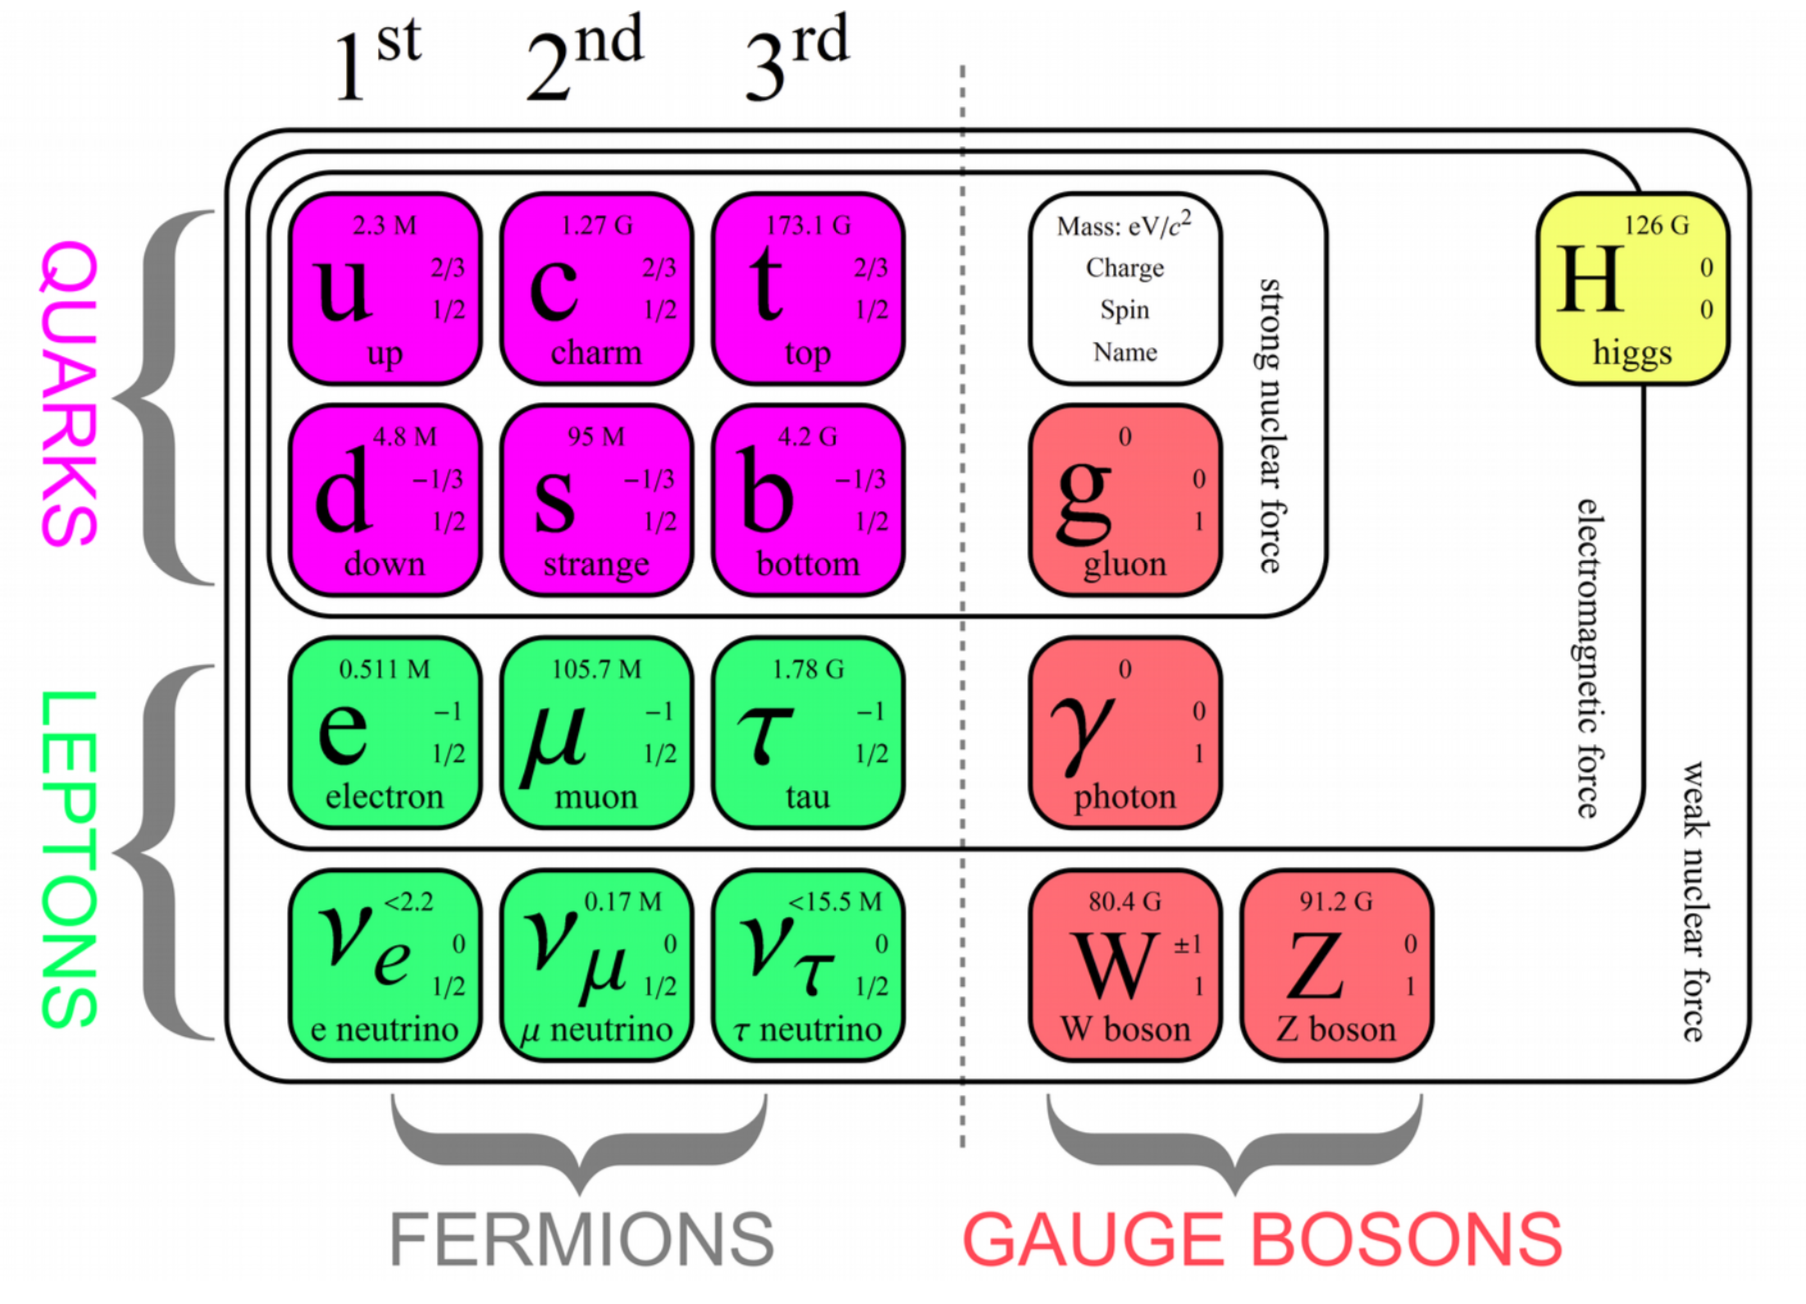
\includegraphics[height=9cm,keepaspectratio]{figures/sm/particular_table_updated.png}
        \caption
            [The elementary particles described by the SM]
            {The elementary particles described by the SM.}
        \label{fig:particular_table}
\end{figure}
%%%%%%%%%%%%%%%%%%%%
matter particles (\emph{fermions}), force-carrying particles (\emph{gauge bosons}), and Higgs bosons.
% ---the only scalar particle so far discovered.
% There are 12 kinds of matter particles (\emph{fermions}), the 4 kinds of force-carrying particles (\emph{gauge bosons}), and the singular kind of Higgs boson---the only scalar particle so far discovered.
% ---of which there are 6 kinds of quarks and 6 kinds of leptons---and the force-carrying particles (gauge \emph{bosons})---of which there are 4 kinds.
There are 12 kinds of fermions which can be split evenly into 2 groups, depending on with which forces they interact:
those that interact via the electromagnetic (EM) force and the weak nuclear force are classified as \emph{leptons}, of which there are 6 kinds (\emph{``flavors''}),
whereas those that interact via the EM, weak, \emph{and} strong nuclear forces are classified as \emph{quarks}, of which there are also 6 flavors.
There are 4 kinds of gauge bosons, each of which is a force carrier for a specific force
(the gluon is said to \emph{mediate} the strong force, the photon mediates the EM force, while the \PWpm and \PZ bosons mediate the weak force).
% Depending on through which forces the particles interact,  split into 6 kinds of \emph{quarks} (strong, weak, and electromagnetic) and 6 kinds of \emph{leptons} (weak and electromagnetic).
% Fermions can be split further into 6 kinds of quarks and 6 kinds of leptons,
% while the 
% only 12 kinds of \emph{matter} particles (green and pink) that comprise all detectable matter,
% 4 \emph{force} particles (red) that convey forces between the matter particles.
Thus, all the diversity and manifestations of reality come from only 17 kinds of ``building blocks''.
% While it is fascinating to wonder how so much diversity can arise from just 17 ``simple'' building blocks, the mission of particle physicists is to understand the underlying mathematical structure that describes Nature in as concise---and accurate---a theory as possible.
It is the mission of particle physicists to understand the underlying mathematical structure that describes Nature in as accurate---and concise---a theory as possible.
The best theory that stands today is called the Standard Model (SM) of particle physics.

%(see Chapter~\ref{ch:theory} for a mathematical overview).
% Universe metastability.
% , the SM accurately describes most of the properties of the eleme
% Although the SM will be mathematically outlined in Chapter~\ref{ch:theory}, it is 
The SM has bore witness to many triumphs over its approximately 70-year development:
it predicted the existence of quarks which were experimentally confirmed in the mid-1970s;
it predicted the existence of the tau neutrino which was experimentally confirmed in 2000;
its most groundbreaking prediction was experimentally confirmed on July 4, 2012---just shy of 10 years ago from the date of this dissertation writing---when the ATLAS and CMS collaborations announced the discovery of the Higgs boson~\cite{chatrchyan_observation_2012, aad_observation_2012, chatrchyan_observation_2013}.

% THE HIGGS IS IMPORTANT BECAUSE it was the missing piece of the SM.
Quantum Field Theory is the mathematical and conceptual backbone of the SM.
Within its framework, all particles are \emph{excitations} of their corresponding field so, \eg \emph{every} electron in the Universe is thought to be an excitation of the one and only electron field that permeates all of spacetime.
The existence of the Higgs boson (\PH) suggests that its corresponding field exists---the \emph{Higgs field}---and, thus, \PH is the quantum excitation of that field.
This all-pervasive Higgs field and its associated boson are generated mathematically via the Brout--Englert--Higgs mechanism (Sec.~\ref{sec:higgs_mech}).
The charged fermions within the SM ``acquire'' their mass by interacting with the Higgs field.
This is also how the Higgs boson itself acquires its mass (\mH)---by interacting with its own field.

% The masses of SM particles \emph{depend} on the value of \mH\ldots \emph{so what is its value?}
Unfortunately, \mH is a free parameter of the SM, so theory is unable to provide a value for \mH based solely on other fundamental constants. % TODO: get mH formula and fix this line.
Thus, \mH must be experimentally measured.
Although \mH has already been measured~\cite{chatrchyan_observation_2012, aad_observation_2012, chatrchyan_observation_2013, PhysRevLett.114.191803, the_cms_collaboration_precise_2015, HIG_16_041, aaboud_measurement_2018, CMS-PAS-HIG-18-029, ATLAS-CONF-2019-025, sirunyan_measurement_2020}, it is important to continually improve the precision on the measurement by lowering the corresponding uncertainties on the mass value.
A more precise value of \mH is two-fold:
first, it improves the theoretical limits on the masses of the other elementary particles and, second, it very well may determine the stability of our universe, as shown in Fig.~\ref{fig:universe_stability}.
% it predicts that all particles---especially the electroweak bosons should be massless
% ,  Particles interact with it and acquire their mass---all except neutrinos and massless bosons.
% Since its conceptualization in 1964, the Higgs boson remained undetected for 48 years until its confirmed production at the LHC. 
%%%%%%%%%%%%%%%%%%%%
\begin{multiFigure}
    \centering
    \addFigure{0.48}{figures/intro/mtop_vs_mH_universestability_zoomout.png}
    \addFigure{0.48}{figures/intro/mtop_vs_mH_universestability_zoomin.png}
    \captionof{figure}
        [Theoretical stability regions of the Universe]
        {Theoretical stability regions of the Universe.
        A) Stability regions of the Universe based on the pole masses of the top quark $\left( \mass{t}^\text{pole} \right)$ and Higgs boson $\left( \mass{h}^\text{pole} \right)$.
        B) Closeup of the SM region in (A).
        The contours represent 68\%, 95\%, and 99\% confidence levels based on the experimental uncertainties of $\mass{t}^\text{pole}$ and $\mass{h}^\text{pole}$.
        Plots taken from~\cite{univ_stab} and units added to all axes.
        }
    \label{fig:universe_stability}
\end{multiFigure}
%%%%%%%%%%%%%%%%%%%%

The production of a Higgs boson is only feasible at conditions close to those thought to exist at the beginning of the Universe.
%   elusive Higgs boson (\PH) is ONLY MADE AT CRAZY CONDITIONS.
This grand achievement is accomplished frequently by the Large Hadron Collider (LHC), located on the border of France and Switzerland.
It is the largest and most powerful proton--proton (\pp) collider ever made.
The LHC accelerates protons to incredible speeds, very close to the speed of light.
When these fast-moving protons collide, the \pp collisions can have a center-of-mass energy as high as 13\TeV.
Newly produced particles spew out of the collision points and are analyzed by detectors like the aforementioned ATLAS and CMS experiments.
These enormous particle detectors have thousands of scientists performing dozens of analyses to look for hints of beyond Standard Model (BSM) physics, extra dimensions, miniature black holes, and more.

This dissertation summarizes the results from two different, but related, analyses.
The first analysis lays out the steps necessary in order to perform the world's best precision measurement of \mH to date, using data collected by the CMS experiment during the LHC Run 2 (2016--2018).
Although this dissertation was completed before the data could be unblinded and before the final measurement of \mH could be made,
expectations on the uncertainties of \mH are set and are predicted to reduce the world's current best precision from 14\MeV down to 11\MeV.
% presents the work done thus far in what is expected to be the world's most precise measurement of \mH.
The second analysis details the search for low-mass dilepton resonances in \htofourl decays and sets limits on related BSM branching fractions and on the Higgs-mixing parameter.
% This dissertation presents the world's most precise measurement of the Higgs boson mass (\mH) to date, using proton--proton collision data from the LHC Run 2, collected and analyzed by the CMS Experiment.

The following chapters of this dissertation begin by describing the function and engineering of the Large Hadron Collider in Chapter~\ref{ch:lhc}.
Then, a thorough description of the CMS experiment and its composite subdetectors is given in Chapter~\ref{ch:cms}.
Next, the first of two analyses---expectations for the precision measurement of the Higgs boson mass using the LHC Run 2 data---is detailed in Chapter~\ref{ch:higgs_mass}.
Afterwards, a the second of two analyses---a search for low-mass dilepton resonances in \htofourl decays---is outlined in Chapter~\ref{ch:dilep_res}.
Finally, the results of the expectations for the Higgs boson mass measurement is summarized in Chapter~\ref{ch:conclusion}.
% begins with a mathematical  the standard model (SM) of particle physics and its mathematical framework, including the Brout-Englert-Higgs (BEH) mechanism

% Chapter~\ref{ch:intro} (\emph{this chapter}) discusses the importance and motivation for measuring the mass of the Higgs boson;
% Chapter~\ref{ch:theory} introduces the standard model (SM) of particle physics and its mathematical framework, including the Brout-Englert-Higgs (BEH) mechanism;
% Chapter~\ref{ch:lhc};
% Chapter~\ref{ch:cms};
% Chapter~\ref{ch:higgs_mass};
% Chapter~\ref{ch:dilep_res};
% Finally, Chapter~\ref{ch:conclusion}.








% Many properties of these particles---and their interactions with each other---are accurately described by the standard model (SM) of particle physics.
% Problematically though, the SM predicts that the gauge bosons (the particles which convey forces) particles are massless.
% The most significant triumph of the SM occurred on July 4$^\text{th}$, 2012 when the ATLAS and CMS collaborations announced the discovery of the ``missing puzzle piece'' of the SM---the Higgs boson.

% This discovery confirmed the SM's prediction that there should exist, which date back to 1964 via the Brout-Englert-Higgs mechanism
% In the SM, particle interactions are conveyed by way of 3 fundamental forces, the strong, weak, and electromagnetic forces, while the 4th force---gravity---is neglected due to its negligible contribution at nuclear distances.
% The seed of the most successful triumph of the SM dates back to 1964, when physicists Robert Brout, François Englert, and Peter Higgs , which occurred on July 4th, 2012, was possible its most spectacular: the when the Higgs boson was  The prediction capabilities of the SM are 
% strong, weak, and electromagnetic interactions
% By understanding the rules by which these particles interact, we can ;
% this is the aim of the Standard Model (SM) of Particle Physics. 
% The Standard Model (SM) is an impressively accurate mathematical theory which describes the fundamental particles of the universe and the rules for their possible interactions.
% 
%  are described mathematically by the impressively accurate Standard Model (SM) of Particle Physics.
% Although there are four fundamental forces of nature, the SM takes into account three of the four forces in nature:
% The Higgs boson (\PH) was the so-called a critical piece of the SM because, without it,  it is the quantum excitation of the so-called Higgs field, an all-pervasive field throughout spacetime 

% It is necessary to scrutinize the properties of this new particle to check whether it truly is the \PH predicted by the SM---or perhaps something else entirely.

% A major shortcoming of the SM is its inability to predict the masses of these particles.

% The SM was not able to predict the masses of these particles until 1964 when the Brout-Englert-Higgs mechanism suggested that 
% It wasn't until 1964 that the Brout-Englert-Higgs mechanism gave a self-consistent way to :
% by breaking the electroweak gauge symmetry of the vacuum would give rise to non-zero masses of the weak gauge bosons.
% This would yield a secondary effect too:
% there should exist a fundamental scalar boson which is the quantum of the so-called ``Higgs field''.
% On July 4th, 2012, this Higgs boson was discovered.
%%%%%%%%%%%%%%%%%%%%%%%%
%--- Standard Model ---%
%%%%%%%%%%%%%%%%%%%%%%%%
\chapter{THE STANDARD MODEL OF PARTICLE PHYSICS}
\label{ch:theory}
The Standard Model (SM) is a collection of the most accurate and self-consistent particle physics theories that mathematically describe the properties of particles within the Universe and their interactions with each other~\cite{Glashow:1961tr,PhysRevLett.19.1264}.
For the past century, some of the most brilliant minds in physics have spent their entire careers to develop equations, mathematical tricks, and completely novel ideas to help build a solid foundation for the SM.

To demonstrate the unparalleled accuracy with which the SM predicts physical phenomena, one needs to look no further than the anomalous magnetic moment of the electron $\left( a_\Pe \right)$.
In 2008, Harvard scientists measured the value to be $a_\Pe^{\text{meas}} = 1.159\,652\,180\,73(28) \times \tentotheminus{3}$~\cite{Hanneke:2008tm},
% \begin{equation*}
%     % a_\Pe^{\text{meas}} = 0.001\,159\,652\,180\,73\,(28)
%     a_\Pe^{\text{meas}} = 1.159\,652\,180\,73\,(28) \times \tentotheminus{3}
% \end{equation*}
where the number in parentheses is the total uncertainty on the measurement.
Meanwhile, the most rigorous calculation of $a_\Pe$ makes use of up to 10 loops using the formalism of quantum electrodynamics (QED) to give a theoretical value of $a_\Pe^{\text{theo}} = 1.159\,652\,182\,031(15)(15)(720) \times \tentotheminus{3}$,
% \begin{equation*}
%     % a_\Pe^{\text{pred}} = 0.001\,159\,652\,182\,031\,(15)(15)(720),
    % a_\Pe^{\text{theo}} = 1.159\,652\,182\,031\,(15)(15)(720),
% \end{equation*}
where the uncertainties in parentheses from left to right are due to the tenth-order QED term, the hadronic contribution, and the fine-structure constant~\cite{Aoyama:2014sxa}.
Comparing $a_\Pe^{\text{meas}}$ to $a_\Pe^{\text{theo}}$ shows an impressive agreement to less than \emph{two parts per trillion}.

The remainder of this chapter presents a general overview of the particles and forces described by the SM (Sec.~\ref{sec:sm_overview}),
followed by a brief analysis of the mathematical underpinnings of the SM, specifically the important process of electroweak symmetry breaking (Sec.~\ref{sec:sm_math}),
and then it concludes by highlighting a few recent measurements that seem to deviate signficantly from SM expectation (Sec.~\ref{sec:shortcomings}).

% TODO: include any of the below?
% MATHEMATICAL FRAMEWORK
% - Show SM Lagrangian.
% - Derive interactions between particles.
%     BEH MECHANISM
%     - Robert Brout, François Englert, and Peter Higgs claimed that elementary particles acquire their masses via spontaneous EWSB. (reword!)
%     - Sheldon Glashow, Abdus Salam, and Steven Weinberg were able to unify the weak and electromagnetic forces into a single force, above the unification energy of 246\GeV.
%     - In 1973 the Gargamelle collaboration experimentally confirmed the existence of the electroweak force by discovering neutral currents in neutrino scattering experiments.
%     - Furthermore, in 1983 the UA1 and UA2 collaborations used proton-antiproton collisions to discover the theorized \PW and \PZ electroweak gauge bosons.
% SHORTCOMINGS OF THE SM

\section{Overview}
\label{sec:sm_overview}

The SM is a renormalizable quantum field theory defined in terms of a Lagrangian (\lagrang) that describes interactions between fundamental particles as governed by the strong, weak, and EM forces.
It is a non-Abelian gauge theory comprising interacting field theories based on gauge invariance and constructed within the framework of quantum mechanics and special relativity.
The SM exhibits invariance under the symmetry group:
\begin{equation*}
    SU(3)_C \times SU(2)_L \times U(1)_Y,
\end{equation*}
where $SU(3)_C$ invariance explains the existence of gluons ($g$) as the mediators of the strong force, described by quantum chromodynamics (QCD), and the $SU(2)_L \times U(1)_Y$ invariance results in the $\PW^\pm$, $\PZ^0$, and $\gamma$ bosons as mediators of the electroweak force, described by the unified electroweak theory and QED.
Interactions via the strong, electromagnetic, and weak forces are restricted to particles carrying a color charge, electric charge, and a weak charge, respectively.
The SM formulation lacks the ability to describe gravity on a quantum level and might actually be incompatible with the most successful modern theories of gravitation.
Gravitational effects are negligible at subnuclear scales.

% Weak hypercharge, weak isospin (L reminds us that this interaction only effects left-handed fermions), color charge
% \textit{Q: What is the difference between $U(1)_q and U(1)_Y$?}
% \textit{Q: Does L stand for left-handed?}

% All observers must Lagrangian 
% The connection between conservation laws and symmetries is best analyzed via Lagrangian mechanics.
% Each Lagrangian has its own set of ``Feynman rules''.

% \textbf{The Particles: The Players on the Fields}
\subsection{The Particles: The Players on the Fields}
Contrary to intuition, fundamental particles are not hard, billiard-ball-like objects as is often perceived.
Instead the SM predicts that every particle is actually an \emph{excitation} of its corresponding field.
So, for example, the electron is an excitation of the \emph{electron field}, $\psi_{\Pe}(x)$, a bispinor that describes a spin-$1/2$ field that follows the equation: 
\begin{equation}
    \left( i\hbar c \gamma^{\mu}{\partial}_{\mu} - mc^{2} \right)\psi_{\Pe}(x) = 0,
    \label{eqn:dirac_notfinished}
\end{equation}
where $\partial_\mu$ is the covariant derivative and $\gamma^\mu$ stands for the Dirac matrices ($\mu = 0,1,2,3$):
\begin{equation}
    \gamma^0 = 
    \begin{pmatrix}
        I_{2} & 0 \\
        0  & -I_{2} \\
    \end{pmatrix}
    \quad , \quad
    \gamma^a = 
    \begin{pmatrix}
        0 & \sigma^a \\
        -\sigma^a  & 0 \\
    \end{pmatrix}
    \quad , \quad \text{for } a = 1,2,3 \quad ,
    \label{eqn:gamma_matrices}
\end{equation}
where $I_2$ is the $2 \times 2$ identity matrix and $\sigma^a$ stands for the typical Pauli matrices:
\begin{equation*}
    \sigma^1 = 
    \begin{pmatrix}
        0 & 1 \\
        1  & 0 \\
    \end{pmatrix}
    \quad , \quad
    \sigma^2 = 
    \begin{pmatrix}
        0 & -i \\
        i  & 0 \\
    \end{pmatrix}
    \quad , \quad
    \sigma^3 = 
    \begin{pmatrix}
        1 & 0 \\
        0  & 1 \\
    \end{pmatrix}
    .
\end{equation*}
By converting to natural units ($c\equiv \hbar \equiv 1$),
extending $\psi_{\Pe}(x) \to \psi$ for the case of any free spin-1/2 Dirac field,
and using `Feynman slash notation' $\left( {\slashed \Omega} \equiv \gamma^\mu \Omega_\mu \right)$ for some operator $\Omega_\mu$,
then \cref{eqn:dirac_notfinished} becomes the familiar and condensed Dirac equation:
\begin{equation}
    \left( i {\slashed \partial} - m \right) \psi = 0.
    \label{eqn:dirac}
\end{equation}
    
In fact, \emph{every} electron is an excitation of this same electron field. 
An electron is identical to every other electron in every way (same mass, same charge, etc.).
Although quantum mechanics (QM) is able to mathematically describe the equations of motions of slow-moving particles, particles with sufficiently high speeds become \emph{relativistic} and are described by the mathematics of special relativity (SR).
When particles move at 30.5\% of the speed of light ($91.4 \times \tentothe{6}$\meter/s), there is a 5\% difference between the particle's rest mass energy ($E = mc^2$) and its relativistic energy ($E = \gamma mc^2$).
No longer does QM describe fast-moving particles; now SR must be used.
The ``merger'' of QM and SR gives rise to quantum field theory (QFT)---the backbone of the SM.

% Figure~\ref{fig:particular_table} shows all the fundamental particles that have been discovered up to the present day.
% The phrase ``fundamental particle'' just means that the particle is not composed of anything smaller than itself. 
% These particles are not just diabolical creations from theorists. 
% No, these particles are precisely defined, mathematical objects whose existence has been predicted by the SM and experimentally verified time and time again in the laboratory.
Every known fundamental particle (Fig.~\ref{fig:particular_table}) has a unique set of properties (like mass, electric charge, spin, \etc) that distinguish it from all the other particles. 
One of the primary goals of particle physics is to determine these properties, because ultimately these properties determine the  \emph{interactions} with one another. 
% Without further ado, let's meet the particles.
The two major types of particles are \emph{bosons} and \emph{fermions}.
% We are going to take a non-traditional route and introduce the bosons first, then the fermions.
% The bosons are said to be the "force carrier" particles. 
% In particle physics, when two particles interact with one another, how do they do it? 
% instead an intermediate particle, very often a boson, is said to ``mediate'' the interaction and be the entity responsible which transfers the force from one particle to the other. 
% Ever wonder how two electrons "know" that they are near each other and that they should repel? 

%%%%%%%%%%%%%%%%%%%%
% TODO: Build Feynman diagram!
\begin{multiFigure}
    \centering
        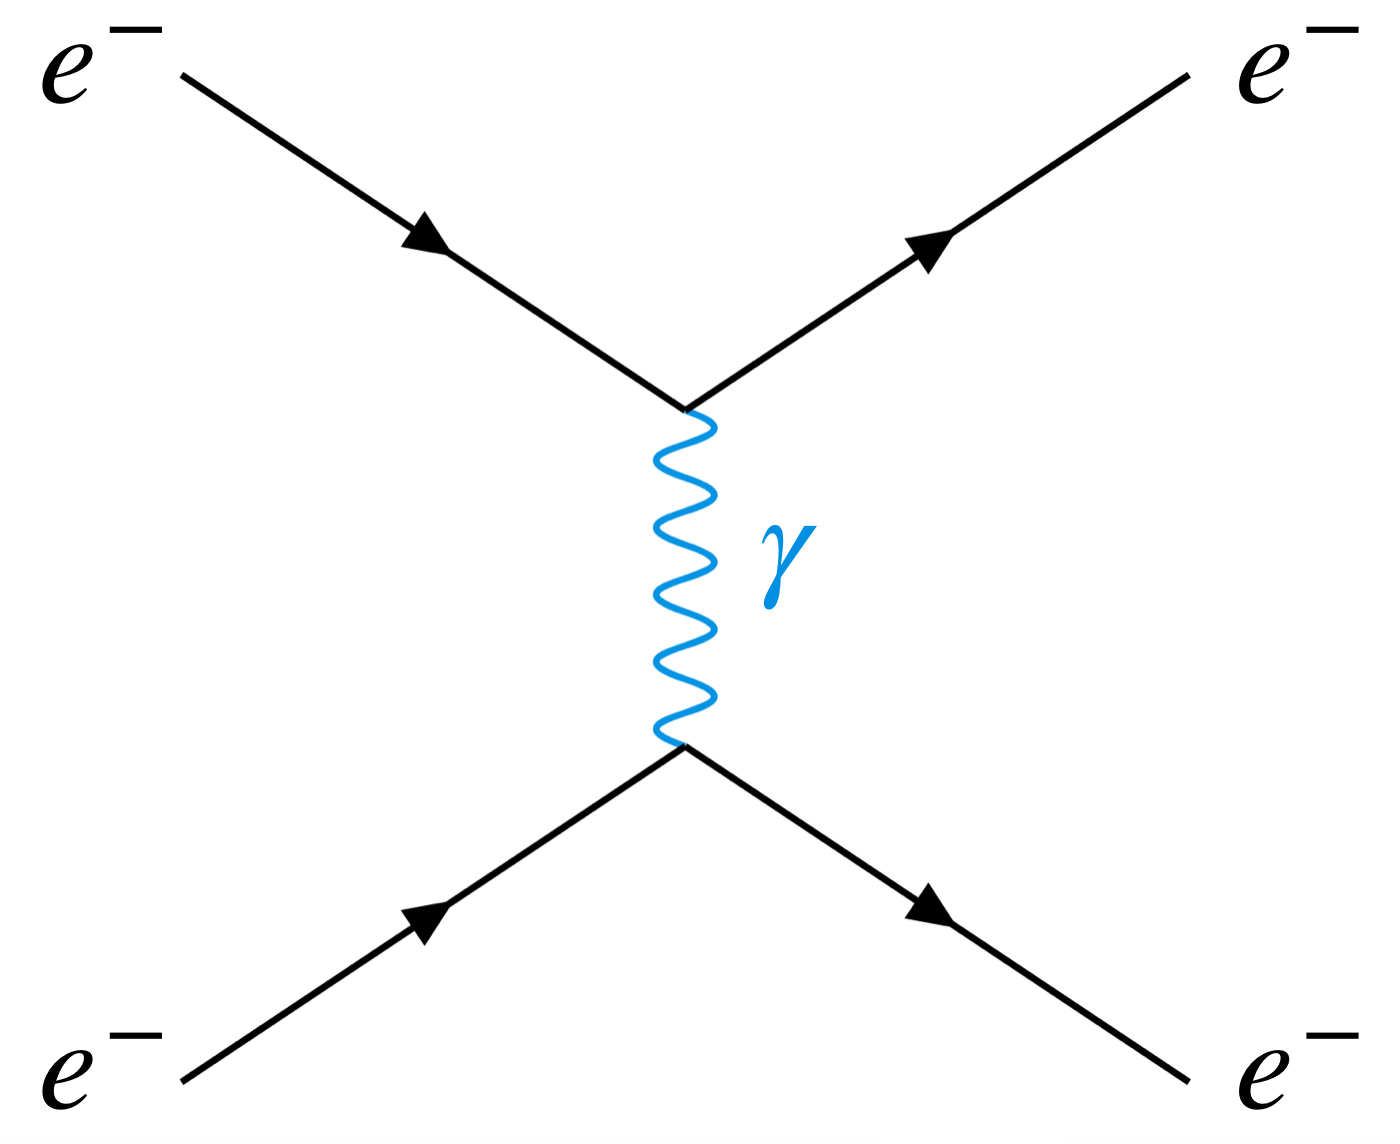
\includegraphics[width=6cm,height=6cm,keepaspectratio]{figures/sm/ee_scattering_moeller.png}
    \captionof{figure}
    \begin{tikzpicture}
        \begin{feynman}[large]
            \centering
            \vertex (h) {$h$}; % h at beginning 
            \vertex [right=1cm of h] (ZZ); % h -> ZZ vertex
            \node [circle, fill=black, inner sep=2pt, above right = 1cm and 1.25cm of ZZ] (Z1); % black dot node at epsilon (control size with ) 
            \node [above left = 7pt and 7pt of Z1] (e) {$\epsilon$}; % node with epsilon text
            \vertex [below right = 1cm and 2.5cm of ZZ] (Z2); % h -> ZZ bottom Z
            \vertex [above right = 0.5cm and 1.25cm of Z2] (Z2l1) {$l$}; % bottom Z -> ll (top l)
            \vertex [below right = 0.5cm and 1.25cm of Z2] (Z2l2) {$l$}; % bottom Z -> ll (bottom l)
            \vertex [above right = 1cm and 1.25cm of Z1] (ZD); % ZD
            \vertex [above right = 0.5cm and 1.25cm of ZD] (ZDl1) {$l$}; % ZD -> ll (top l)
            \vertex [below right = 0.5cm and 1.25cm of ZD] (ZDl2) {$l$}; % ZD -> ll (bottom l)
            \diagram* {
                (h) -- [scalar] (ZZ),
                (ZZ) -- [boson, edge label=$Z$] (Z1),
                (ZZ) -- [boson, edge label=$Z$] (Z2),
                (Z1) -- [boson, edge label=$Z_D$] (ZD),
                (ZDl2) -- [fermion] (ZD) -- [fermion] (ZDl1);
                (Z2l2) -- [fermion] (Z2) -- [fermion] (Z2l1);
            };
        \end{feynman}
    \end{tikzpicture}
        [Feynman diagram showing electron--electron (Møller) scattering]
        {Feynman diagram showing electron--electron (Møller) scattering.} 
    \label{fig:ee_scattering}
\end{multiFigure}
%%%%%%%%%%%%%%%%%%%%

\subsubsection{Bosons: Use the Force}

\emph{How do two electrons ``know'' that one is near the other and that they should repel?}
\Cref{fig:ee_scattering} shows a Feynman diagram of two electrons interacting with one other by means of an intermediate, virtual photon $(\gamma)$.
In QFT, mediator particles are called bosons---like the photon---convey interactions beween two interacting electrons.
The idea is that the photon carries momentum away from the first electron and carries it to the second one, therefore making it appear as if the two electrons are repelling one another.
The photon is not a measurable particle in this case, so it is said to be a \emph{virtual} photon.
This is why gauge bosons are often called the force carriers.

% Quantum Electrodynamics, one of the theories cooped up in the SM, is a quantum field theory that can mathematically describe one electron "throwing" a photon to the other.
The Feynman diagram in Fig.~\ref{fig:ee_scattering} is a simple way to visualize particle physics processes, although it must be stated that it does not depict what \emph{actually} happens between particles.
Feynman diagrams are instead a useful tool to help calculate the probabilities with which various processes happen.
Each diagram represents a single, scalar number that is calculated from a QFT integral and indicates how likely a process is to happen.
% Another benefit of Feynman Diagrams is their tinker-toy-like connectab you can string them together in novel ways to predict real-world processes.
Thus, QED is able to calculate the probability the electrons mediating such a photon between them. 
It's not just limited to electrons mediating photons, however.
The prediction capabilities of QED and other QFTs reach astounding accuracy how likely a process is to happen, between whichever particles and fields. 
One just needs to know the particle properties first.
% \emph{Any} particle with electric charge can interact via the electromagnetic force (EM) force.

Thus, the first force carrier---the first gauge boson---has been presented: the photon.
It is a massless particle and it is the mediator of the EM force. 
Photons only interact with particles that carry \emph{electric charge}.
The kind of charge that a particle carries ultimately determines with which bosons it may interact and via which forces.
The four fundamental forces found in nature are (in order of decreasing relative strength):
\begin{enumerate}
    \item strong force: $\mathcal{O}(1)$
    \item EM force: $\mathcal{O}(10^{-2})$
    \item weak force: $\mathcal{O}(10^{-13})$
    \item gravitational force: $\mathcal{O}(10^{-38})$
\end{enumerate}

\emph{If the photon mediates the EM force, then what mediates the other forces?}
The mediators of the strong force are the 8 gluons. 
Similar to the photon, they are also massless.
Gluons are trapped inside of protons, neutrons, and other hadronic matter. 
They `glue' nuclei to together, hence their name.
Just as photons only interact with particles that have electric charge, gluons only interact with particles that have \emph{color} charge.
There are three kinds of color charges---red, green, and blue---though not at all related to everyday visual color.
Each color has its corresponding anticolor charge---antired, antigreen, and antiblue---which negates the corresponding color charge, much like how a `$+1$' electric charge neutralizes a `$-1$' charge.
Not only would a red--antired (or green--antigreen or blue--antiblue) charge pair be considered a colorless (neutral) state but so too would the combination of red--green--blue (or antired--antigreen--antiblue).
A phenomenon known as \emph{color confinement} suggests that only colorless bound states are observable.
Interestingly, gluons themselves carry color charge (typically a color--anticolor combination) which they mediate between quarks (fermions discussed below).  % TODO: This may be repeated below.
This is in direct contrast to the photon which does not itself carry its associated charge (the electric charge).

There are three bosons which mediate the weak force: the \PZ, $\PW^+$, and $\PW^-$.
They are extraordinarily massive particles, weighing in at $91.2\GeV$ for the \PZ and $80.4\GeV$ for both kinds of \PW bosons. 
That means the W bosons has more mass than an iron atom!
These bosons interact with any particle that carries ``weak hypercharge'' ($Y_W$).
% The weak force has plagued physicists for nearly a century until only recently.
Particles which decay via the weak force live an astonishingly long time. 
Take for example the decay of a neutral pion into two photons:
$\pi^0 \to \gamma \gamma$. 
The decay occurs \emph{very} quickly---$\mathcal{O}(\tentotheminus{18}\snd)$---because it is mediated by the EM force.
Now consider the decay of a charged kaon into 3 charged pions:
$K^+ \to \pi^+ \pi^+ \pi^-$.
This decay occurs \emph{much} more slowly---$\mathcal{O}(\tentotheminus{8}\snd)$---compared to the $\pi^0$ decay.
The difference of over 10 orders of magnitude is because the charged kaon decayed via the weak force (in this example).

The final boson is the scalar Higgs boson and will be introduced in Sec.~\ref{sec:higgs_mech}.

% 1. There are 12 kinds fermions which are the matter particles and comprise all the matter that you see and feel
% 2. And in the other group there are 5 kinds of bosons, which are the force carriers and help fermions communicate with each other. 

\subsubsection{Fermions: Each One Matters}
There are 12 kinds of fermions, which are the matter particles of the Universe.
Fermions have half-integer spin, typically a value of $1/2$, and can be split into one of two groups, depending on if they interact with the strong force (quarks) or not (leptons).
First, the leptons are explored below, followed by the quarks.

\textbf{Leptons:}
% Ultimately all the matter we see, feel, and interact with daily is composed of fermions.
% Referring back to Fig.~\ref{fig:particular_table}, Fermions can be categorized into two groups: \textbf{leptons} and \textbf{quarks}.
One lepton was already introduced earlier: the electron (\Pe).
Looking again at the ``particular table'' (Fig.~\ref{fig:particular_table}), the electron has a ``cousin'' that is 200 times more massive than itself: the muon (\Pmu).
There is yet a lepton sibling even more massive than the \Pe or \Pmu: the tauon ($\tau$). 
All three of these leptons have the familiar $-1$ charge which allows them to interact via the EM force and exchange photons with other electrically charged particles.

The charged leptons also carry weak hypercharge, which allows them to interact via the weak force. 
If a charged lepton interacts with a \PWpm boson, it transforms into its corresponding ``partner''---the other member of the $SU(2)$ isospin doublet, the neutrino ($\nu$).
These fickle neutrinos \emph{only} interact via the weak force (and supposedly gravity) so they are effectively invisible, \ie very difficult to detect.
% They are very difficult to detect.

% How do we know that some particles, like protons and neutrons are actually composed of smaller bits, like these up and down quarks?
% Through deep inelastic scattering experiments, analogous to the Rutherford experiment,
% one can shoot electrons at these nucleons and probe into them.
% Thanks to the wave-particle duality of nature, these electrons can act like little wave bullets,
% that tunnel into the nucleon and sometimes... they bounce back. 

% For each charged lepton, it can transform it into its neutral form: 
% the corresponding neutrino. 
% For example, the muon can transform into a muon neutrino - and vice versa.
% To undergo this transformation, the muon must interact 
% with the appropriate boson: W-. 
% This conserves electric charge at this vertex.

% You can also view this diagram from another perspective 
% by rotating it. 
% Here we see a 

\textbf{Quarks:}
The six quarks are the fermions which interact with gluons.
They have \st{quarky} quirky names like: 
up, down, charm, strange, top, bottom. 
These are called the six ``flavors'' of quarks.
The top quark is an absolutely massive particle, being at the \emph{top} of the particle mass scale at $172.25^{+0.76}_{-0.77}\GeV$~\cite{Tumasyan:2779091}---approximately the same mass as a tungsten atom.

Quarks (\Pq) are electrically charged particles, but they have fractional charge.
Each quark in the top row of Fig.~\ref{fig:particular_table} has $+2/3$ electric charge and the bottom row has $-1/3$.
This is why combining two up quarks with a down quark to form a proton yields a net electric charge of $+1$.

Just as the leptons carried weak hypercharge and could interact via the weak force, so too can quarks. 
The $\PW^{\pm}$ bosons can change one flavor of quark into another.
The \PZ boson only affects the spin, momentum, and energy of the particle with which it interacts.

In addition to electric charge, quarks also carry one kind of color charge, which allows them to interact with gluons via the strong force. 
Quarks combine in different ways to form at least two types of hadrons.
The first (second) type of hadron is the \emph{baryon} (\emph{meson}), which is a particle that contains a combination of 3 (2) colorless quarks/antiquarks.
Examples of baryons are the familiar proton, consisting of the three-quark bound state $\Pqu \Pqu \Pqd$, and the neutron, consisting of the three-quark bound state $\Pqu \Pqd \Pqd$.
Examples of mesons are the pion $\pi^+$ $\left(\Pqu \Paqd \right)$\footnote{
    \textbf{Antiparticles:} Most particles have a corresponding \emph{antiparticle}, whose charges (\eg color charge, electric charge) are the opposite of the original particle's.
    Sometimes the notation for the antiparticle is obvious, like in the case of the electron $\left( \Pem \right)$ whose antiparticle is the positron $\left( \Pep \right)$.
    Other times, the common notation is to indicate an antiparticle with a \emph{bar} symbol over the letter, as is the case for a general quark (\Pq) and its corresponding antiquark $\left( \Paq \right)$
    Accounting for leptons, quarks, bosons, quark bound states, and now antiparticles, it's easy to see why it's called the ``\emph{particle zoo!}''
}, the kaon $K^-$ $\left(\Pqs \Paqu \right)$, and the $\jpsi$ $\left( \Pqc \Paqc \right)$.

\section{Mathematical Underpinnings of the SM}
\label{sec:sm_math}

Thanks to the brilliance of Professor Emmy Noether~\cite{Noether1918}, physics has greatly benefitted from the study of \emph{symmetry}.
She showed that the very existence of a symmetry \emph{implies} the conservation of an associated quantity (typically called a `current').
For example, if some law of physics is the same on Earth as it is on Mars (\eg $E = mc^2$ \emph{is} still true even across vast amounts of space), then there is an inherent symmetry (or ``sameness'') to the system across space and this \emph{implies} that the system obeys \emph{conservation of linear momentum}.
Similarly, if a system has rotational symmetry (\eg if you perform an experiment and get the same results facing north as you do facing southeast), then this \emph{implies} that the system obeys \emph{conservation of angular momentum}.
As a final---and astounding---example, a system that shows symmetry across time implies \emph{conservation of energy} within that system.

Particle physics makes use of \emph{gauge} symmetries, which lead to conservation of electric charge, color charge, \etc
By understanding such symmetries, the equations of motion (EOM) for a system are revealed (\ie how the system evolves throughout spacetime).
In particle physics, Newtonian mechanics is insufficient to obtain the EOM of quantum particles, so instead Lagrangian mechanics is used.
The first step is to write down the Euler--Lagrange equation~\cite{Halzen:1984mc}:
\begin{equation}
    % TODO: Use proper partial fractions commands from physics package.
    \frac{d}{\dt}
    \left( \frac{\partial \lagrang}{\partial \dot{q}_i} \right)
    -
    \frac{\partial \lagrang}{\partial q_i} = 0,
    \label{eqn:euler_lagrange}
\end{equation}
where the $q_i(t)$ are the time-dependent generalized coordinates of the associated particles
and \lagrang is the general Lagrangian function defined as:
\begin{equation*}
    \lagrang \equiv T - V,
\end{equation*}
where $T$ and $V$ are, respectively, the kinetic and potential energy functions of the system.
The second step is to find the stationary points using \cref{eqn:euler_lagrange} which yields the EOM of the system.

In particle physics, however, the generalized coordinates are promoted to particle \emph{wave functions}---functions of space and time:
\begin{align*}
    q_i(t) \to \phi(\vec{x}, t) & \equiv \phi(x_\mu)
    \\
    \lagrang(q_i, \dot{q}_i, t) \to  \lagrangdens & \left( \phi, \frac{\partial \phi}{\partial x_\mu}, x_\mu \right),
\end{align*}
where \lagrangdens is called the `Lagrangian density',
the idea being that at every point in space there is an associated value of \lagrang that still depends on time and the dynamical variables of the associated particles.
The Lagrangian density is related to \lagrang via:
\begin{equation*}
    \lagrang = \int{d^3x \, \lagrangdens}.
\end{equation*}
Gauge transformations can be applied to particle fields so long as \lagrangdens \emph{remains invariant}.

In all its glory, the SM Lagrangian density is given by~\cite{Halzen:1984mc, thesis_xunwu}:
\begin{align*}
    \lagrangdens =
    & - \frac{1}{4} B_{\mu \nu} B^{\mu \nu} - \frac{1}{4} W^a_{\mu \nu} W^{a \mu \nu} - \frac{1}{4} G^k_{\mu \nu} G^{k \mu \nu}
    \\
    & + \abs{D_\mu\Phi}^2 + \mu^2 \Phi^\dagger \Phi - \lambda \left( \Phi^\dagger \Phi \right)^2
    \\
    & + \sum_f{
        % \left[
            \bar{\psi}^f_R \left(i {\slashed D_\mu}\right) \psi_R^f + \bar{\psi}^f_L \left(i {\slashed D_\mu}\right) \psi_L^f
        % \right]
        }
    \\
    & + \sum_f{
        % \left[
            g_f \left[ \bar{\psi}_R^f \Phi^\dagger \psi_L^f + \bar{\psi}_L^f \Phi \psi_R^f + \bar{\psi}_R^f \tilde{\Phi}^\dagger \psi_L^f + \bar{\psi}_L^f \tilde{\Phi} \psi_R^f \right]
        % \right]
        },
\end{align*}
where the field strength tensors ($B_{\mu \nu}$, $W_{\mu \nu}^a$, $G_{\mu \nu}^k$) for their corresponding interaction fields
($B_\mu$, $W_\mu^a$, $G_\mu^k$)
of their associated symmetry groups are given by:
\begin{align*}
    U(1) : \quad & B_{\mu \nu}    = \partial_\mu B_\nu - \partial_\nu B_\mu
    \\
    SU(2) : \quad & W_{\mu \nu}^a  = \partial_\mu W_\nu^a - \partial_\nu W_\mu^a + g \varepsilon^{abc} W_\mu^b W_\nu^c
    \\
    SU(3) : \quad & G_{\mu \nu}^k  = \partial_\mu G_\nu^k - \partial_\nu G_\mu^k + g_s f^{klm} G_\mu^l G_\nu^m,
\end{align*}
where the slash notation is borrowed from \cref{eqn:dirac} and the gauge-transformed covariant derivative ($D_\mu$) is given by:
\begin{equation*}
    D_\mu = \partial_\mu - i g^\prime B_\mu Y - i g W_\mu^a T^a - i g_s G_\mu^k t^k,
\end{equation*}
where $g^\prime$ ($Y$), $g$ ($T^a$), and $g_s$ ($t^k$) are the field strength coefficients (interaction operators) for the $U(1)$, $SU(2)$, and $SU(3)$ groups, respectively,
and $\varepsilon^{abc}$ and $f^{klm}$ are the structure constants of the $SU(2)$ and $SU(3)$ groups which determine the group generators via:
\begin{align*}
     \left[ T^a, T^b \right] &= i \varepsilon^{abc} T_c
     \\
     \left[ t^k, t^l \right] &= i f^{klm} t_m
\end{align*}
% \Phi, \Phi^\dagger, \mu, \lambda,
% \psi_R^f, \bar{\psi}_R^f
where $a$ runs from 1--3 (from \cref{eqn:gamma_matrices}),
$k$ stands for the group generator indices and runs from 1--8,
% and finally the sums are taken over the fermion flavors $f$, and for each coupling there exists a coupling strength $g_f$.



% The main objective of the LHC is to probe the Electroweak Symmetry Breaking (EWSB) mechanism that generates the masses of the known elementary particles in the SM.
%  in the SMby the ATLAS~\cite{ATLAS:2012yve} and the CMS~\cite{CMS:2012qbp} collaborations and the subsequent studies of its properties with the full data set from Run 1, from 2009 to 2012, with a center-of-mass energy of 7\TeV and 8\TeV, provided the first opportunity to study this mechanism.
The discovery of the Higgs boson in 2012 confirmed the existence of the Higgs field, subsequently providing insight into the mechanism from which EWSB arises.
Not only does it explain the short-range nature of weak interactions but it also provides an explanation for the massive \PWpm and \PZ gauge bosons.

In the SM, the electroweak interactions are described by a gauge field theory invariant under the $SU(2)_L \times U(1)_Y$ symmetry group.
The mechanism of EWSB provides a general framework to preserve the structure of these gauge interactions at high energies~\cite{PhysRevD.2.1285, PhysRevLett.13.321, PhysRev.145.1156}.
The EWSB mechanism posits a self-interacting electroweak doublet of complex scalar fields, whose CP-even neutral component acquires a vacuum expectation value (VEV), which sets the scale of the symmetry breaking.
Four massless Goldstone bosons are generated, two of which linearly combine to give the \PWp and \PWm gauge bosons while the remaining two combine to give the photon $(\gamma)$ and the \PZ gauge bosons.
The masses of all fermions are also a consequence of EWSB since the Higgs field is postulated to couple to the fermions through Yukawa interactions.

\subsection{The Brout--Englert--Higgs Mechanism}
\label{sec:higgs_mech}

The SM lagrangian contains a scalar potential term that reads:
\begin{equation}
    V (\phi) = \mu^2\phi^\dagger\phi + \lambda(\phi^\dagger\phi)^2,
    \label{eqn:scalar_pot}
\end{equation}
where the Higgs field $\left( \phi(x) \right)$ is a self-interacting $SU(2)_L$ doublet of complex scalar fields containing 4 real degrees of freedom $\left( \phi^k \text{, where } k=1, 2, 3, 4 \right)$ with weak hypercharge $Y = 1$:
\begin{equation}
    \phi(x) = \frac{1}{\sqrt{2}}
    \begin{pmatrix}
        \sqrt{2}\phi^+ \\
        \phi^3 + i\phi^4
    \end{pmatrix},
    \label{eqn:higgs_doublet}
\end{equation}
where $\phi^3$ and $\phi^4$ are the CP-even and CP-odd neutral components, $\phi^+ \equiv \phi^1 + i \phi^2$ is the complex charged component of the Higgs doublet, and $V(\phi)$ is the most general renormalizable scalar potential.
The hypercharge is normalized such that $Q = T_{3} + \frac{Y}{2}$, where $Q$ is the electric charge and $T_{3}$ is the eigenvalue of the diagonal generator of $SU(2)_L$.

The case where $\lambda > 0$ in \cref{eqn:scalar_pot} indicates that a minimum exists in the potential and that $\phi$ is self-coupling~\cite{bass_higgs_2021}.
If $\mu^2 < 0$ is also required, then the minimum of $V(\phi)$ $\left( \ie \frac{\partial V}{\partial \phi} = 0 \right)$ occurs at:
\begin{equation}
    \abs{\phi} = \sqrt{ \frac{-\mu^2}{2\lambda} }.
    \label{eqn:higgs_min}
\end{equation}
% \begin{align*}
%     &\frac{\partial V}{\partial \phi} = 0
%     \\
%     \implies \abs{\phi} = &\sqrt{ \frac{-\mu^2}{2\lambda} }  \equiv \frac{v}{2},
% \end{align*}
This corresponds to the manifold of points that are invariant under the $SU(2)$ transformations~\cite{Halzen:1984mc}.
This ``Maxican hat'' potential is shown in \cref{fig:mex_hat} and illustrates the concept of spontaneous symmetry breaking.
%%%%%%%%%%%%%%%%%%%%
\begin{multiFigure}
    \centering
        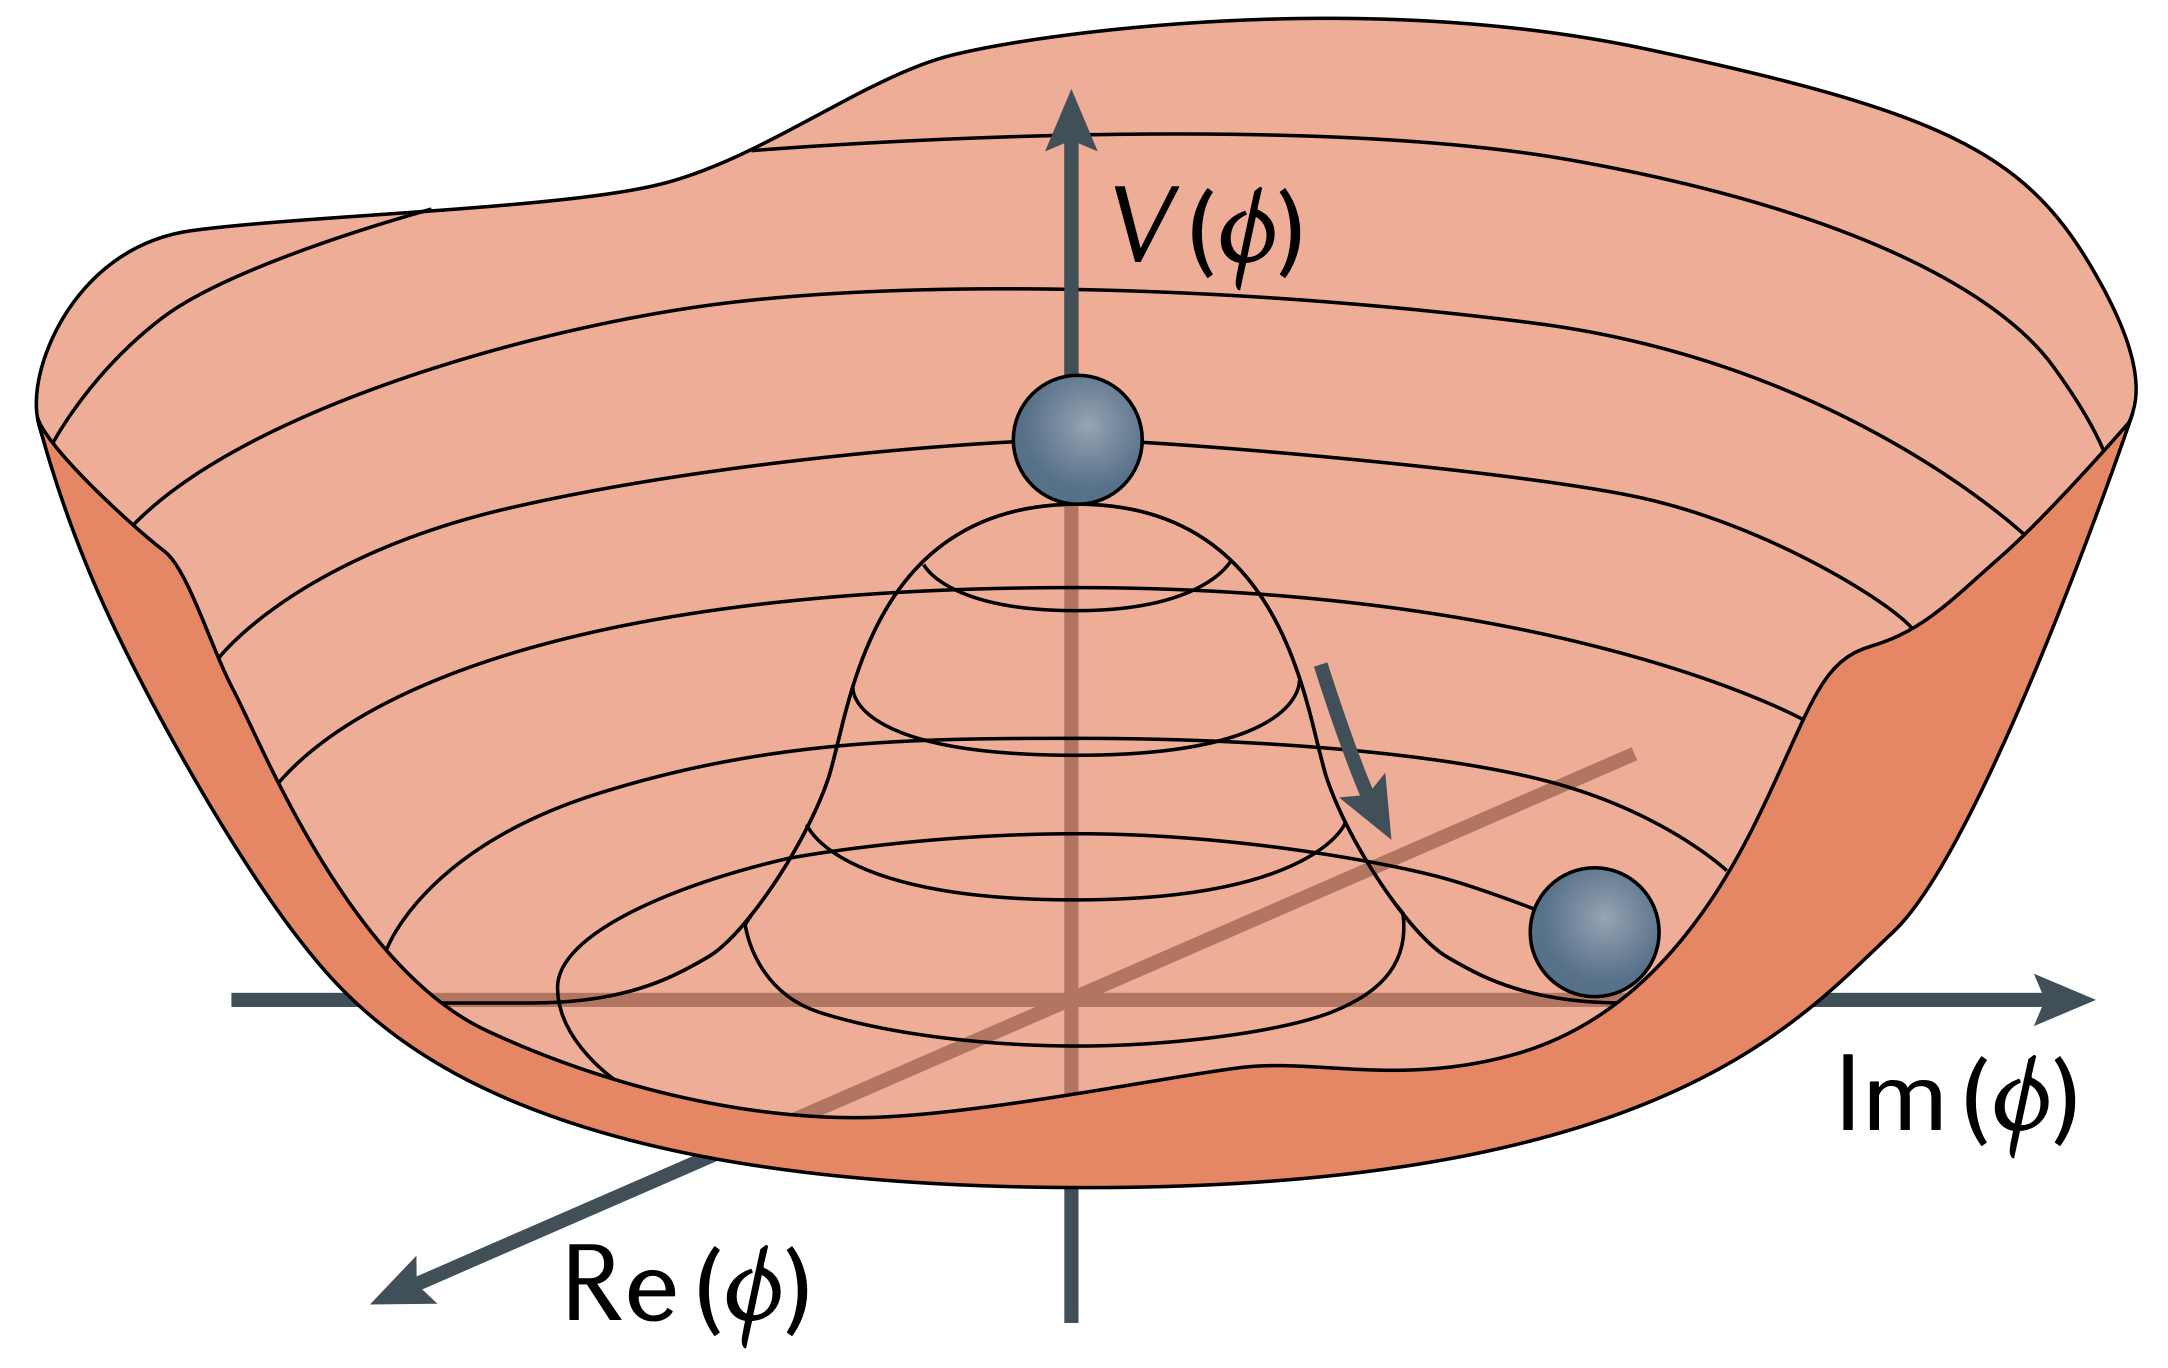
\includegraphics[height=6cm,keepaspectratio]{figures/sm/higgs_potential.png}
    \captionof{figure}
        [Mexican-hat-shaped Higgs potential for $\lambda > 0$ and $\mu^2 < 0$]
        {Mexican-hat-shaped Higgs potential for $\lambda > 0$ and $\mu^2 < 0$.
        Figure taken from~\cite{bass_higgs_2021}.} 
    \label{fig:mex_hat}
\end{multiFigure}
%%%%%%%%%%%%%%%%%%%%
Choosing the point $\phi^1 = \phi^2 = \phi^4 = 0$ in the manifold for convenience constrains $\left(\phi^3\right)^2 = \frac{-\mu^2}{\lambda} \equiv v^2$,
where $v$ is the Higgs VEV and has a value of 246\GeV. % TODO: Ref VEV value.
The doublet in Eqn.~\ref{eqn:higgs_doublet} can now be written as:
\begin{equation*}
    \langle\phi\rangle = \sqrt{\frac{1}{2}}
    \hspace{3pt}
    \begin{pmatrix}
        0 
        \\
        v 
    \end{pmatrix},
\end{equation*}
and expansion of $\phi(x)$ about this particular vacuum gives:
\begin{equation*}
    \phi(x) = 
    \sqrt{ \frac{1}{2} }
    \hspace{3pt}
    \begin{pmatrix}
        0
        \\
        v + H(x)
    \end{pmatrix},
\end{equation*}
where $H(x)$ is the scalar Higgs field.
Spontaneous breaking of the SM gauge symmetry $SU(3)_C \times SU(2)_L \times U(1)_Y$ into $SU(3)_C \times U(1)_\text{EM}$ has now been induced.

The global minimum of the theory defines the ground state, and spontaneous symmetry breaking implies that there is a global or local symmetry of the system that is not respected by the ground state.
From the four generators of the $SU(2)_L \times U(1)_Y$ SM gauge group, three are spontaneously broken, implying that they lead to non-trivial transformations of the ground state and indicate the existence of three massless Goldstone bosons identified with three of the four Higgs field degrees of freedom.
The Higgs field couples to the $W_\mu$ and $B_\mu$ gauge fields associated with the $SU(2)_L \times U(1)_Y$ local symmetry through the covariant derivative appearing in the kinetic term of the Higgs Lagrangian:
\begin{equation*}
    \lagrang_\text{Higgs} = (D_\mu\phi)^\dagger(D^\mu\phi) - V(\phi),
\end{equation*}
where $D_\mu\phi \equiv \left( \partial_\mu - ig \frac{\sigma^a}{2}W^a_\mu - ig^\prime \frac{Y}{2} B_\mu \right)\phi$,
and $\sigma^a$ (with $a = 1,2,3$) are the usual Pauli matrices,
and finally $g$ and $g^\prime$ are the $SU(2)_L$ and $U(1)_Y$ gauge couplings, respectively,
It is useful to note that:
\begin{equation*}
    \frac{g^\prime}{g} = \tan{\theta_W},
\end{equation*}
where $\theta_W$ is the weak mixing angle, which has been measured to be~\cite{noauthor_precision_2006}:
\begin{equation*}
    \sin^2{\theta_W} = 0.231\,53 \pm 0.000\,16,
\end{equation*}
though other measurements of $\theta_W$ have been performed~\cite{the_lhcb_collaboration_measurement_2015, cms_collaboration_measurement_2018}.
As a result, the neutral and the two charged massless Goldstone degrees of freedom mix with the gauge fields corresponding to the broken generators of $SU(2)_L$ and $U(1)_Y$:
\begin{align*}
    A_\mu &= B_\mu \cos{\theta_W}  + W^3_\mu \sin{\theta_W},
    \\
    Z_\mu &= -B_\mu \sin{\theta_W}  + W^3_\mu \cos{\theta_W},
\end{align*}
thus becoming, in the unitary gauge, the longitudinal components of the $\PZ$ and $\PW$ physical gauge bosons, respectively. % TODO: I don't think this is correct.
The $\PW$ and $\PZ$ gauge bosons acquire masses:
\begin{equation*}
    m_{\PW} = \frac{1}{2}vg, \hspace{7pt} m_{\PZ} = \frac{1}{2} v \sqrt{g^2+{g^\prime}^2},
\end{equation*}
from which the following relation is derived:
\begin{equation*}
    \frac{m_{\PW}}{m_{\PZ}} = \cos{\theta_W}.
\end{equation*}

The fourth generator remains unbroken since it is the one associated to the conserved $U(1)_\text{EM}$ gauge symmetry; thus, its corresponding gauge field---the photon ($\gamma$)---remains massless.
Similarly the eight color gauge bosons, the gluons ($g$), corresponding to the conserved $SU(3)_C$ gauge symmetry with 8 unbroken generators, also remain massless (though confined inside hadrons and mesons as the result of the asymptotic freedom behaviour of QCD).
Hence, from the initial four degrees of freedom of the Higgs field, two are absorbed by the $\PW^\pm$ gauge bosons, one by the $\PZ$ gauge boson, and the one remaining degree of freedom, $\PH$, is the physical Higgs boson---a relatively new and eponymous scalar particle dreamt of by Peter Higgs~\cite{PhysRevLett.13.321,PhysRev.145.1156}.
The Higgs boson is neutral under the electromagnetic interactions and transforms as a singlet under $SU(3)_C$ and hence does not couple at tree level to the massless photons and gluons.

The fermions of the SM acquire mass through renormalizable interactions between the Higgs field and the fermions, \ie the Yukawa interactions:
\begin{equation*}
    -\lagrang_\text{Yukawa} = \hat{h}^{(d)}_{ij} \bar{q}_{L_i} \phi d_{R_j} +
    \hat{h}^{(u)}_{ij} \bar{q}_{L_i} \tilde{\phi} u_{R_j} +
    \hat{h}^{(\ell)}_{ij} \bar{\ell}_{L_i} \phi e_{R_j} + h.c.,
\end{equation*}
which respect the symmetries of the SM but generate fermion masses once EWSB occurs.
The indices $i,j = 1,2,3$ refer to the three families of up quarks, down quarks, or charged leptons.
In the Lagrangian above, $\tilde{\phi} = i\sigma_2\phi^*$ while $q_L$ ($\ell_L$) and $u_R$, $d_R$ ($e_R$) are the quark (lepton) $SU(2)_L$ doublets and singlets, respectively, while in each term $\hat{h}^{(f)}_{{ij}}$ is parameterized by a $3\times3$ coupling matrix for the appropriate fermion ($f$).
% The mass term for neutrinos is omitted, but could be added in an analogous manner to the up-type quarks when right-handed neutrinos are supplementing the SM particle content (neutrinos can also acquire Majorana masses via non-renormalizable dimension-5 interactions with the Higgs field~\cite{Weinberg:1979sa}).
Once the Higgs field acquires a VEV, and after rotation to the fermion mass eigenstate basis that also diagonalizes the Higgs--fermion interactions, $\hat{h}^{(f)}_{ij} \rightarrow h^{(f)}_{i} \delta_{ij}$, all fermions acquire a mass given by:
\begin{equation*}
    m^{(f)}_{i} = \frac{h^{(f)}_{i} v}{\sqrt{2}}.
\end{equation*}
Finally, looking back at the first two terms of Eqn.~\ref{eqn:scalar_pot} reveals the mass of the SM Higgs boson $(\mH)$ in terms of the parameters $v$ and $\lambda$:
\begin{equation*}
    \mH = \sqrt{2 \lambda} v.
\end{equation*}
It should be noted that the EWSB mechanism provides no additional insight into possible underlying reasons for the large variety of masses of the fermions, often referred to as the \emph{flavor hierarchy}.
The fermion masses, accounting for a large number of the free parameters of the SM, are simply translated into Yukawa couplings.



% % At room temperature, we know that the weak force, which mediates decays of radioactive substances, is very different from the EM force.
% % However, at large energy scales, like those found during the Big Bang or those produced in the energetic proton--proton collisions of the Large Hadron Collider, the electromagnetic (EM) force and weak force are unified. 
% At large energy scales, like those found during the Big Bang or those produced in the energetic proton--proton collisions of the Large Hadron Collider, the electromagnetic (EM) force and weak nuclear force are one and the same: they are unified.
% However, at lower temperatures (like room temperature for example), we know that the weak force is very different from the EM force.
% The former mediates decays of radioactive substances, whereas the latter mediates the excitation of electrons in an atom.
% So what is responsible for the separation of these two forces, this so-called \emph{electroweak symmetry breaking}?

% Upon writing down the equations of motion from the SM Lagrangian (easier said than done), one discovers that all the particles mentioned earlier should have \emph{no mass}.
% Well that's a problem because most particles in nature definitely have mass, like the quarks, leptons, W$^{\pm}$, and Z bosons.
% % Since mass is a scalar, one can introduce a scalar field (spin 0) into the Lagrangian.
% By introducing a complex SU(2) doublet of scalar fields into the SM Lagrangian, in such a way that it leaves the Lagrangian invariant, then all peace can be restored.
% This scalar field turns out to be the Higgs field, and its excitations are Higgs bosons.
% Doing so reveals the particle which should have mass,
% The process of introducing a Higgs field and breaking the electroweak symmetry is called the \textbf{Higgs Mechanism}.

% % The Higgs field is required to be a scalar field and consists of a complex doublet, with four degrees of freedom.
% Each particle interacts with the Higgs field with a different strength: in fact, a particle's coupling strength to the Higgs field is exactly its mass! 
% The more the particle interacts with the Higgs field, the more mass it gains.
% Excitations, or quanta, of the Higgs field are Higgs bosons and are a direct consequence of introducing a Higgs scalar field into the SM Lagrangian to allow particles to have mass.


% \begin{itemize}
%     \item strong force $(1)$
%     \item EM force $(10^{-1})$
%     \item weak force $(10^{-13})$
%     \item gravitational force $(10^{-40})$
% \end{itemize}
% Speaking of forces, the four fundamental forces found in nature, along with their decreasing, relative strength are: 

% \textbf{Electroweak Interaction}
% Particles can interact with one another at long range.
% For example, an electron can emit a photon which can travel a 

% Electromagnetic force and weak force were unified Electroweak symmetry.
% This introduced 4 electroweak bosons: the photon, Z, W+, and W-.
% Then lectroweak symmetry breaking happened.
% This made the photon massless and the Z, W+, and W- as (very) massive.

% \textbf{Higgs Mechanism}
% Force field that fills space in the whole Universe but has no source or direction.
% The field has the same field at every point.
% It's a scalar field with spin 0.
% It does have electroweak charge.

\section{Shortcomings of the SM}
\label{sec:shortcomings}

More and more experimental measurements are being published that present results which significantly deviate from SM predictions.
One such measurement comes from the Collider Detector at Fermilab (CDF) Collaboration, which recently measured the mass of the \PW boson $(\mass{\PW})$ to be $80\,433.5 \pm 9.4\MeV$, whereas the SM predicts a mass of $80\,357 \pm 4\MeV$---a discrepancy of 7.0 standard deviations~\cite{cdf_collaboration_high-precision_2022}.
The CDF measurement of \mass{\PW}, along with measurements performed by other collaborations, is shown in Fig.~\ref{fig:wmass}.
%%%%%%%%%%%%%%%%%%%%
\begin{multiFigure}
    \centering
        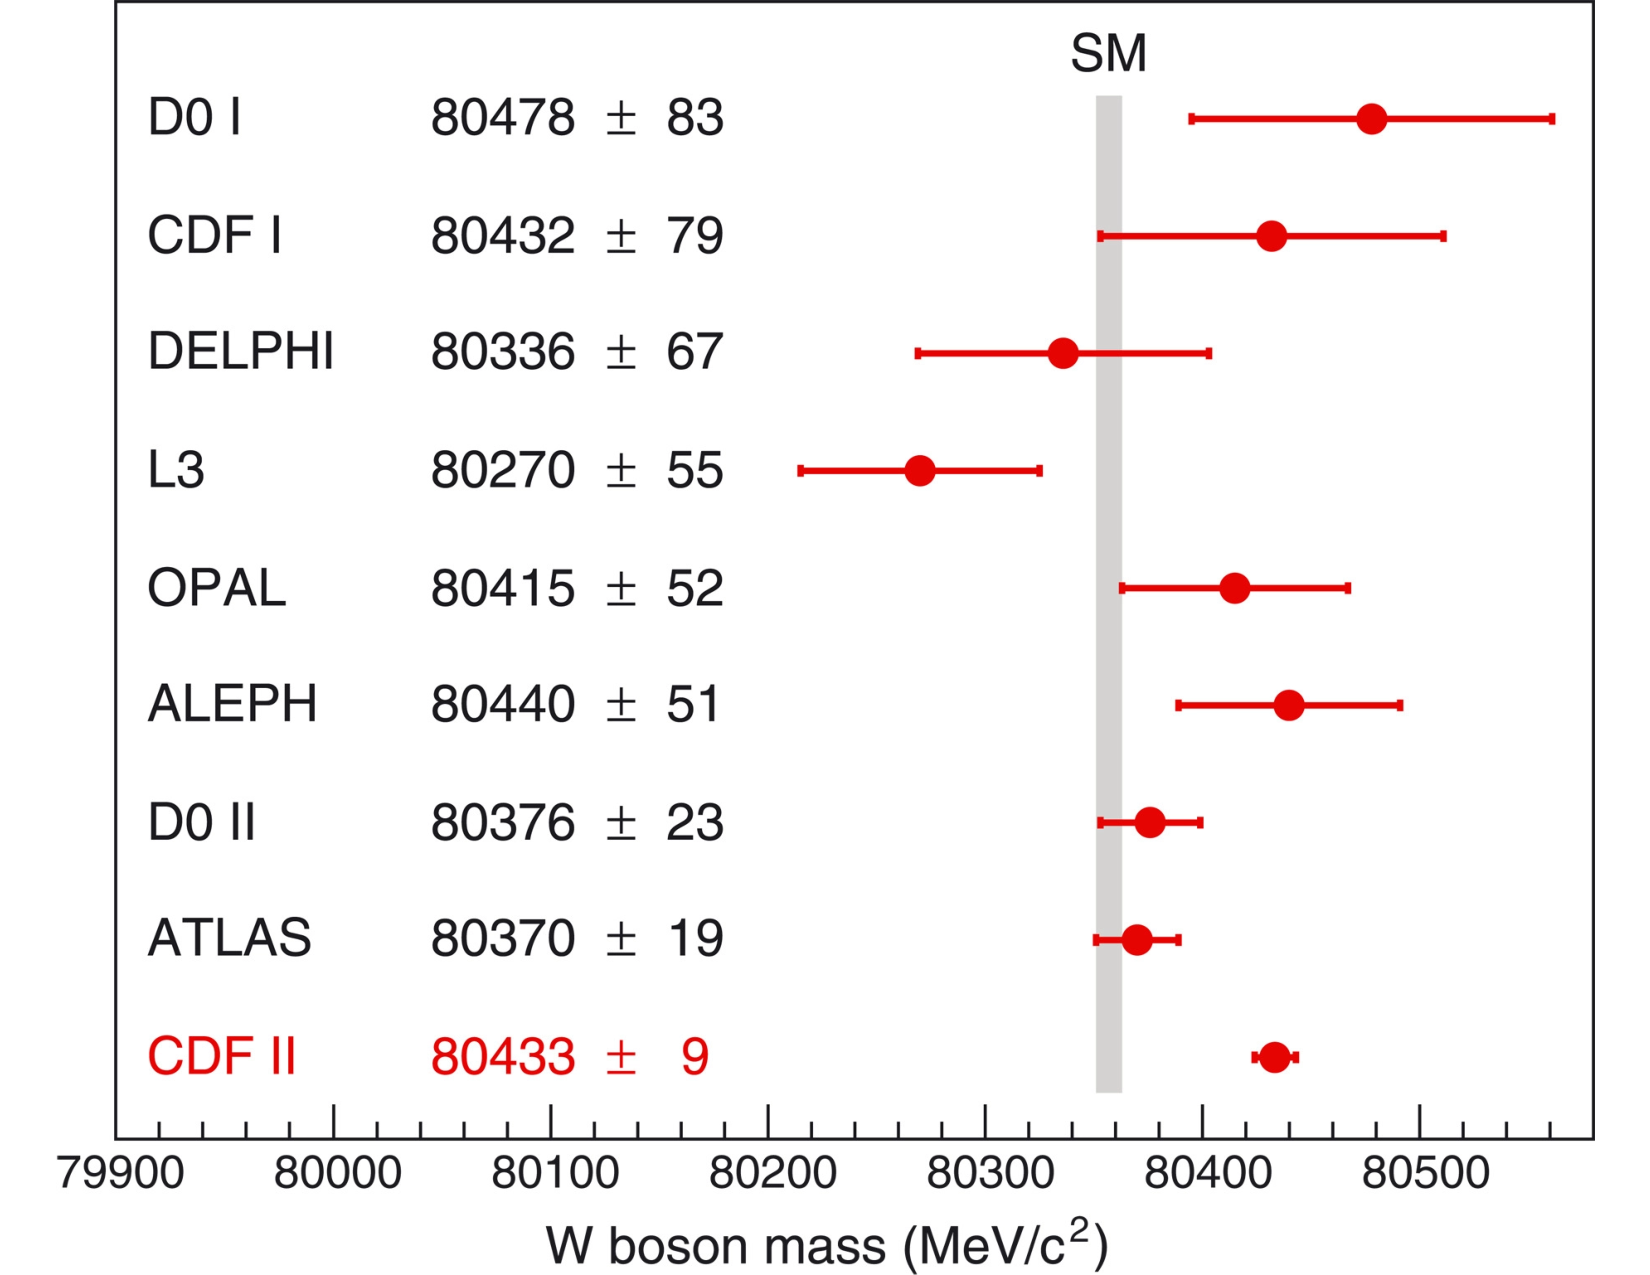
\includegraphics[height=8cm,keepaspectratio]{figures/sm/wmass.pdf}
    \captionof{figure}
        [Precision measurements of the \PW boson mass performed by various collaborations]
        {Precision measurements of the \PW boson mass performed by various collaborations.
        Plot taken from~\cite{cdf_collaboration_high-precision_2022}.} 
    \label{fig:wmass}
\end{multiFigure}
%%%%%%%%%%%%%%%%%%%%
Another recent result comes from the Baksan Experiment on Sterile Transitions, which suggests that electron neutrinos oscillate between sterile neutrino states~\cite{PhysRevLett.128.232501}.

Moreover, fermion masses are not predicted by the SM;
their masses are parameters of the theory and so must be experimentally measured~\cite{Halzen:1984mc}.
Additionally, the SM does not
\begin{itemize}
    \item \ldots incorporate gravity on a mathematical quantum level
    \item \ldots explain the matter/antimatter asymmetry of the Universe
    \item \ldots predict the existence of dark matter
    \item \ldots explain why there should be exactly three generations of fermions~\cite{particle_data_group_review_2020}.
\end{itemize}

Therefore, the foundation of the SM must continue to be scrutinized via particle collider experiments.
Hadrons are a reasonable choice for particle collisions, since hadronic matter is full of constituent parts---appropriately called \emph{partons}---like quarks and gluons.
By im\emph{part}ing immense amounts of energy into the partons and smashing them together, this allows the partons to interact and convert their energies into new kinds of matter.
One of the primary grounds of investigation to test the SM is at the world's largest circular particle collider: the Large Hadron Collider (Ch.~\ref{ch:lhc}).

%%%%%%%%%%%%%
%--- LHC ---%
%%%%%%%%%%%%%
% % Great animation about protons going through the CERN accelerator complex.
% https://www.youtube.com/watch?v=FLrEghnKncA

\chapter{THE LARGE HADRON COLLIDER}
\label{ch:lhc}

% OUTLINE
% \section{Motivation for a Large Hadron Collider}
\section{Motivation}
Although the SM (Ch.~\ref{ch:theory}) has shown to be an astoundingly accurate framework so far, it must continue to be scrutinized by the barrage of measurements that either confirm or contradict its predictions.
% cross-examined
Interestingly, a recent measurement of the mass of the \PW boson has shown significant deviation from SM predictions, with a sensitivity of 7$\sigma$~\cite{cdf_collaboration_high-precision_2022}.
After all, undeniable fact comes from reproducible results obtained from measurement---not from some theoretical model which \emph{may} or \emph{may not} describe reality.
Whenever results from measurement contradict the predictions made by a model, the model must necessarily be cast aside and replaced by one whose predictions are in alignment with truth, \ie \emph{measurement}.
% the truth of Nature

So how \emph{are} measurements obtained in the realm of particle physics?
% be continuously tested for its accuracy.
% Must be shaken by the results of experiment to see if its foundation is stable.
% So far, it has upheld against the onslaught of measurements but must be continuously tested for accuracy.
% , it does not explain many phenomena observed in the universe, as discussed in ().
% Although the SM (Chapter~\ref{ch:theory}) is an astoundingly accurate framework, it does not explain many phenomena observed in the universe, as discussed in ().
% As discussed in TODO:PROBLEMS WITH SM, there is observed physics that has not yet been explained in a coherent theoretical and mathematical framework.
% There are currently many searches for physics \emph{beyond the standard model} (BSM) which may explain certain observed physical phenomena that .
% robust, elegant, and accurate (so far), 
% perhaps there is physics beyond the SM (BSM).
% After all, the truth of Nature comes from the results of measurements---not from mathematical and theoretical models.
% Although the standard model (SM) of particle physics  is rather elegant
% and  for the physical phenomena that it does explain.
Modern day physicists study the fundamental constituents of matter and their interactions by using state-of-the-art technologies combined with time-tested methodologies:
%  is to do it the same way humans have been doing it for centuries:
by smashing tiny bits of matter together to turn them into even \emph{tinier} bits.
Such is the purpose of the world's largest and most powerful particle accelerator---the Large Hadron Collider (LHC).
% CERN on a map.
%%%%%%%%%%%%%%%%%%%%
\begin{multiFigure}
    \centering
    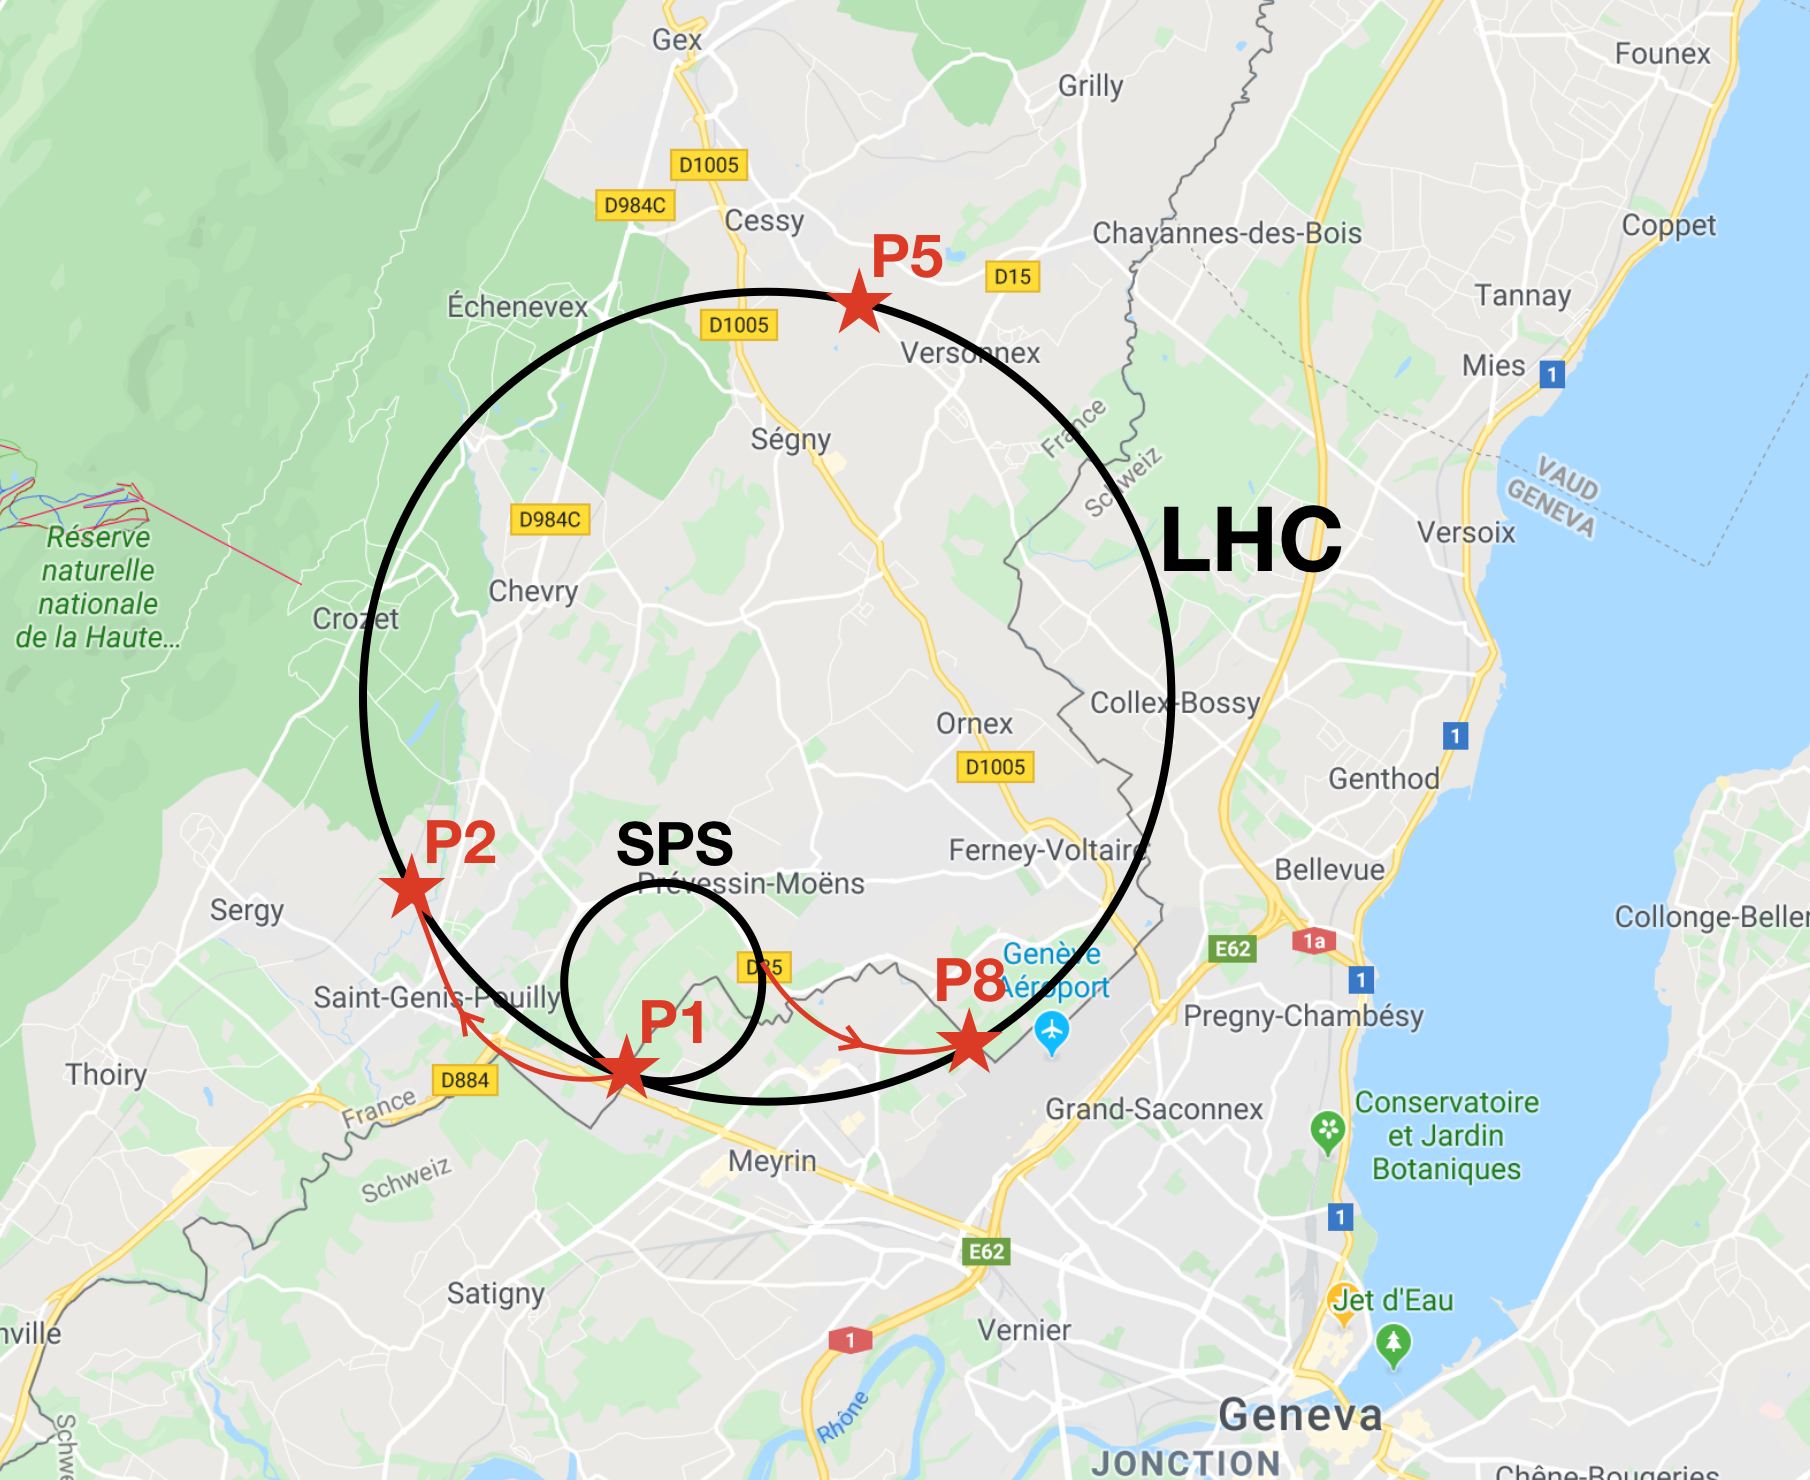
\includegraphics[height=8cm]{figures/lhc/lhc_drawn_on_map_withpoints.png}
    \captionof{figure}
        [The LHC ring superimposed on a map]
        {The LHC (bigger black ring) and Super Proton Synchrotron (SPS, smaller black ring) are drawn to scale, with the neighboring town of Geneva (bottom-right) for size comparison. 
        The four red stars indicate the \pp collision points along the LHC. 
        }
    \label{fig:lhc_on_map}
\end{multiFigure}
%%%%%%%%%%%%%%%%%%%%

\section{The LHC at CERN}
% The circular LHC ring straddles the Franco-Swiss border, approximately 100\meter below the surface of the earth
% (Fig.~\ref{fig:lhc_and_boosters}, Left).
% The ring itself has a circumference of 26.7\Km, making its inscribed area (56.7$\Km^{2}$) almost four times greater than the area of the neighboring city of Geneva (15.9$\Km^{2}$).
% This machine is not only a particle accelerator but also a proton--proton (\pp) collider, sending one beam of protons travelling clockwise and the other beam counterclockwise around the ring. 
Deep beneath the surface of the earth (50--175\meter), the LHC straddles the border shared by France and Switzerland.
Sandwiched between the scenic Jura mountains to the northwest and the sprawling city of Geneva (French: Genève) to the southeast is CERN.
To illustrate the enormous circumference (26.659\Km) of this circular accelerator, Fig.~\ref{fig:lhc_on_map} shows the LHC superimposed to scale on a map.
For reference, the inscribed area of the LHC (56.7$\Km^{2}$) is almost four times greater than the area of the neighboring city of Geneva (15.9$\Km^{2}$)\footnote{
    By now, the astute reader may have noticed that the author prefers to use the unit prefix `K' to represent $\tentothe{3}$ instead of the typical lowercase `k'.
    \emph{But why}, you may ask?
    The author invites the reader to consider that within the International System of Units (SI), the common unit prefixes that represent a collection of more than 1 base unit are \emph{uppercase} letters: 
    \eg `M' is mega-- $(\tentothe{6})$,
    `G' is giga-- $(\tentothe{9})$,
    `T' is tera-- $(\tentothe{12})$, \etc---except for arguably the most commonly used letter: `k' for kilo $(\tentothe{3})$.
    Frustrating.

    Furthermore, consider the usage of ``KJ'' on page 6 in Ref.~\cite{collaboration_cms_2008}.
    Lastly, recall that three zeros in finance are sometimes condensed to a simple `K', \eg \$20\,000 becomes \$20K.
    Thus, the author chooses consistency over convention and kindly warns the reader to anticipate `K' for `kilo--', such as `\Kgns' to represent 1000 grams, instead of `kg'.
    
    The diehard defender of SI may argue that a kilobyte (KB) is 1024 bytes and is typically represented as `KB'.
    True, so in order to maintain self-consistency within this dissertation, the value 1024 will be represented as `k';
    so a kilobyte will be represented as `kB', though it is not used in this dissertation. 
}.

The LHC is not only a particle \emph{accelerator} but also a proton--proton (\pp), proton--lead ion, and lead--lead ion \emph{collider}.
By sending one particle beam clockwise around the ring and the other beam counterclockwise, the charged particles are carefully maneuvered using dipole magnets and tightly collimated using quadrupole magnets before they ultimately collide at 4 specific points along the LHC, as shown in Fig.~\ref{fig:lhc_on_map}.
% , anywhere from , , and sandwiched between the scenic Jura mountains to the west and the sprawling city of Geneva (Genève) to the east
%  straddles the Franco-Swiss border, approximately 100\meter below the surface of the earth (Fig.~\ref{fig:lhc_and_boosters}, Left).
When the LHC is fully powered, \emph{each} proton in the beam carries an average energy of 6.5\TeV which gives a single \pp collision a massive\footnote{
    For comparison, a \emph{mosquito} in flight carries about 13\TeV of kinetic energy.
    For two \emph{fundamental particles} to collide with this much energy is truly astonishing!
} center-of-mass energy of 13\TeV.
This emulates the conditions theorized to exist at the beginning of the universe, which allows cosmological studies to be carried out.
The hugely energetic \pp collisions cause the quark and gluon constituents within the protons to interact with each other and transform into new particles.
The newly created particles and the residual particle debris are ejected away from the collision point---whether straight down the beampipe, completely orthogonal to it, or somewhere in between.
Massive particle detectors are stationed at each of the 4 collision points to detect the outgoing particle ``spray''.
The 4 main particle detectors and their locations along the LHC are:
\begin{itemize}
    \item A Toroidal LHC ApparatuS (ATLAS)---located at the first collision point, ``P1''
    \item A Large Ion Collider Experiment (ALICE)---located at P2
    \item the Compact Muon Solenoid (CMS, Chapter~\ref{ch:cms}) experiment---located at P5
    \item the LHC-beauty (LHCb) experiment---located at P8
\end{itemize}
% TODO: Get rid of extra newline that appears after itemize.
% ATLAS	A Toroidal LHC Apparatus
% CMS	Compact Muon Solenoid
% LHCb	LHC-beauty
% ALICE	A Large Ion Collider Experiment
% TOTEM	Total Cross Section, Elastic Scattering and Diffraction Dissociation
% LHCf	LHC-forward
% MoEDAL	Monopole and Exotics Detector At the LHC
% FASER	ForwArd Search ExpeRiment
% SND	Scattering and Neutrino Detector

The world-renowned feat of digging the tunnel for, constructing, commissioning, and monitoring the LHC was made possible by CERN:
the European Organization for Nuclear Research (French: \emph{Conseil Européean pour la Recherche Nucléaire}).
CERN is an international collaboration of---at the time of this writing---more than 33 countries,
% it's actually 34.
% Learn about the series of accelerators here:
% https://cdsweb.cern.ch/record/2771424/files/CERNAnnualReport_2020_EN.pdf
each of which is considered either a Member State, an Associate Member State, or an Observer.
The complex of CERN (Fig.~\ref{fig:lhc_complex}) is located just to the west of P1 and is akin to a small science \emph{city}---complete with many offices, manufacturing facilities, and experiments such as the Antiproton Decelerator (AD), the Neutrons Time of Flight (n$\_$TOF), and the Isotope Separator OnLine (ISOLDE) experiments.
% the world's largest and most powerful particle accelerator, the Large Hadron Collider (LHC).
% The completion of this world-renowned feat was only possible through the careful efforts of thousands of scientists, engineers, administrators, \etc from all over the world.
% At the time of this writing, CERN is associated with at least 33 countries, each of which is considered either a Member State, an Associate Member State, or an Observer.
Although the LHC is the most famous of the accelerators at CERN, its fame is only made possible by a series of smaller and lesser-known accelerators that \emph{feed} the LHC.
% would not be able to accelerate \emph{any} charged particles from rest; not collide particles at such massive energies if not for the lesser-known accelerators that feed into the LHC.
% but it takes clever engineering and a series of smaller accelerators to eventually feed particles into the LHC to reach their maximum energy of 6.5\TeV.
Therefore, a natural way to explore the intricacies and inner workings of the LHC is to follow the path of one of its ``inhabitants''---a single proton---as it makes its way to and through the gigantic collider.
% Accelerator complex at CERN.
%%%%%%%%%%%%%%%%%%%%
\begin{multiFigure}
    \centering
    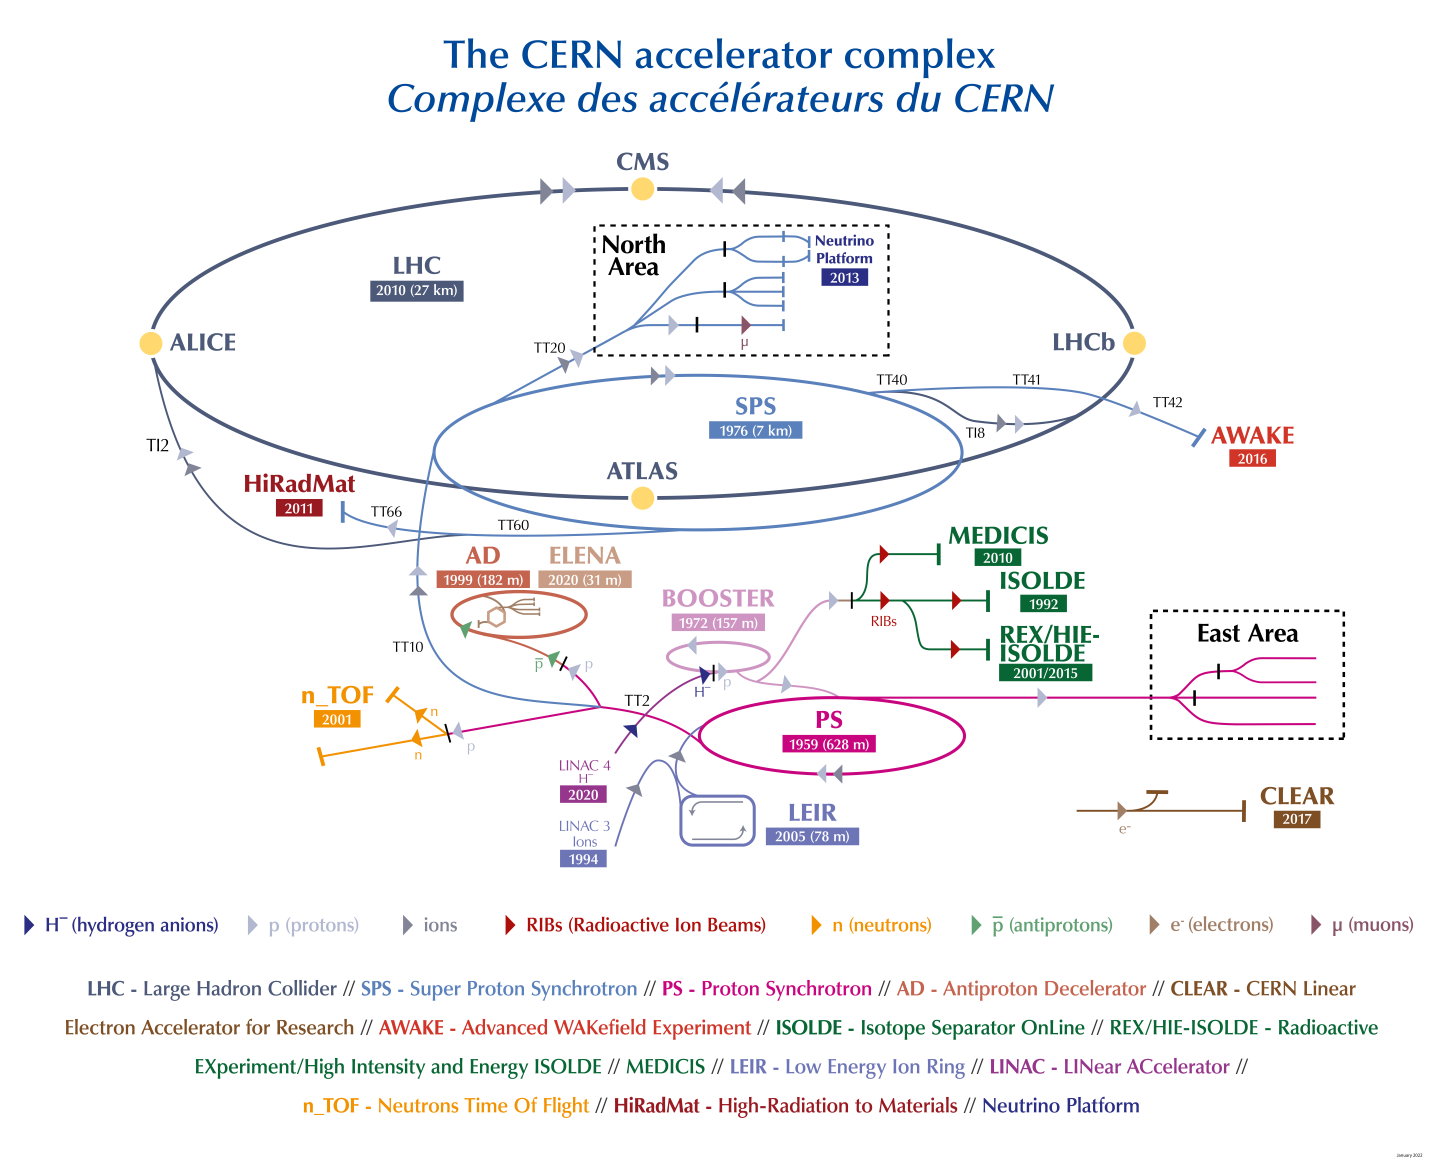
\includegraphics[height=12.5cm]{figures/lhc/cern_complex.png}
    \captionof{figure}
        [The accelerator complex at CERN]
        {The accelerator complex at CERN. Figure taken from~\cite{cern_complex}.}
    \label{fig:lhc_complex}
\end{multiFigure}
%%%%%%%%%%%%%%%%%%%%

\section{The Journey of a Proton at the LHC}
The journey to discovery begins with a surprisingly small tank of hydrogen gas (\htwo) located in the LINAC4 building at the main CERN site.
% , in which a proton that is bound to another proton as a molecule of H2 .
% Pic of hydrogen source from here: https://www.lhc-closer.es/taking_a_closer_look_at_lhc/0.linac4
Inside this tank of \htwo are on the order of $\tentothe{23}$ protons and let's keep track of, say, the $n^\text{th}$ proton as it makes its \emph{first} journey around the LHC---let's call this one \pname (from the Greek word \textgreek{πρώτος} meaning \emph{first}).
% TODO:DOUBLE CHECK THIS
% coexist in bound states as molecules of H$_2$.
Although the tank has a meager mass of 
% TODO: Double check this number.
$\approx$10\Kg,
it has enough protons inside to keep the LHC colliding protons for over \emph{200\,000 years} of constant operation.

\pname and the rest get injected into a series of increasingly larger and more powerful accelerators.
They begin their journey at the \emph{Linac4}---a linear particle accelerator---that converts the particles into hydride ions (H$^-$) and then accelerates them to 160\MeV, at which point, they are fed into the \emph{Proton Synchrotron Booster} (PSB).
In the PSB, each H$^-$ has its electron pair completely stripped away, leaving only the bare proton ($\Pp^+$).
\pname then enters a series of circular accelerators, where each machine feeds its protons into the next in order to increase the proton center-of-mass energy by at least 1 order of magnitude with each feeding.
The flow of accelerators is as follows:
\begin{itemize}
    % TODO: mention electric field?
    % \item The flow 
    \item From the PSB, \pname are the rest are accelerated to 2\GeV and then injected into the \emph{Proton Synchrotron} (PS).
    \item The PS increases the energy of the particles to 26\GeV and then feeds the protons into the \emph{Super Proton Synchrotron} (SPS).
    \item Next, the SPS energizes the protons to a beam energy of 450\GeV and sends protons in discrete packets (\emph{proton bunches}), each of which contains $\mathcal{O}(\tentothe{11})$ protons into the LHC. %  $\approx$$\tentothe{11}$  are packed together into a ``proton bunch''. % a accelerates protons to com energy
\end{itemize}
% TODO: Mention: A single proton bunch is about the size of a human hair ($\approx$50\mum wide and $\approx$10\cm long). 
% TODO: Mention: The clockwise and counterclockwise rings are filled to a maximum of 2808 proton bunches, each one spaced 25\ns apart, and then sent to collide. 
It is inside the LHC that \pname and its fellow protons within its proton bunch are given precisely timed \emph{kicks} by electric fields\footnote{
    The electric field quickly oscillates between pointing parallel to the direction of travel of the proton bunch to pointing \emph{antiparallel} to the direction of travel.
    Therefore, precise timing is required to ensure that the electric field only points parallel so as to speed up the protons in the proton bunch.
    This is analgous to the timing required when pushing a person on a swing:
    the pusher must push at \emph{just} the right time to increase the momentum of the one swinging, lest the pusher slows the swinger down!
} within radio-frequency (RF) cavities.
After sufficient energy is delivered to the proton bunches, the particles reach their max speed of 0.999\,999\,990$c$ (corresponding to a Lorentz factor of $\gamma \approx 7000$). %  Wikipedia says 6930.  99.999\,996\%$c$.
At this speed, \emph{each proton} in the proton bunch carries an energy as measured in the lab frame of 6.5\TeV.

\pname and its neighboring protons in the proton bunch are nearly ready for a head-on collision with another proton bunch to make interesting physics.
The only problem is that the proton bunches must be turned (to keep them in the circular LHC) and must be tightly squeezed down (to increase the chance of \pp collisions).
Since the protons are bare, they are all positively charged, and are subject to a Lorentz force when they pass through a magnetic field.
Therefore, the LHC is equipped with 1232 dipole magnets distributed all along its circumference to turn the proton bunches.
The cross section of such a dipole magnet is shown in Fig.~\ref{fig:lhc_dipole_xs}.
Each dipole magnet is 14.3\meter long, weighs 35\tonne, costs nearly 500\,KCHF to produce, and has nearly 11\,700\,A of current running through it.
Only with such massive currents is it possible to generate the necessary magnetic field strength of 8\tesla to keep the protons moving in a circular fashion at their near-light speed. 
The magnetic field is maintained by copper-clad niobium-titanium coils, which requires the cryogenics conditions of 96\tonne of superfluid helium-4 to achieve the necessary temperature of 1.9\kelvin to reach a superconducting state; 
this temperature is colder than that of outer space.
%%%%%%%%%%%%%%%%%%%%
\begin{multiFigure}
\centering
    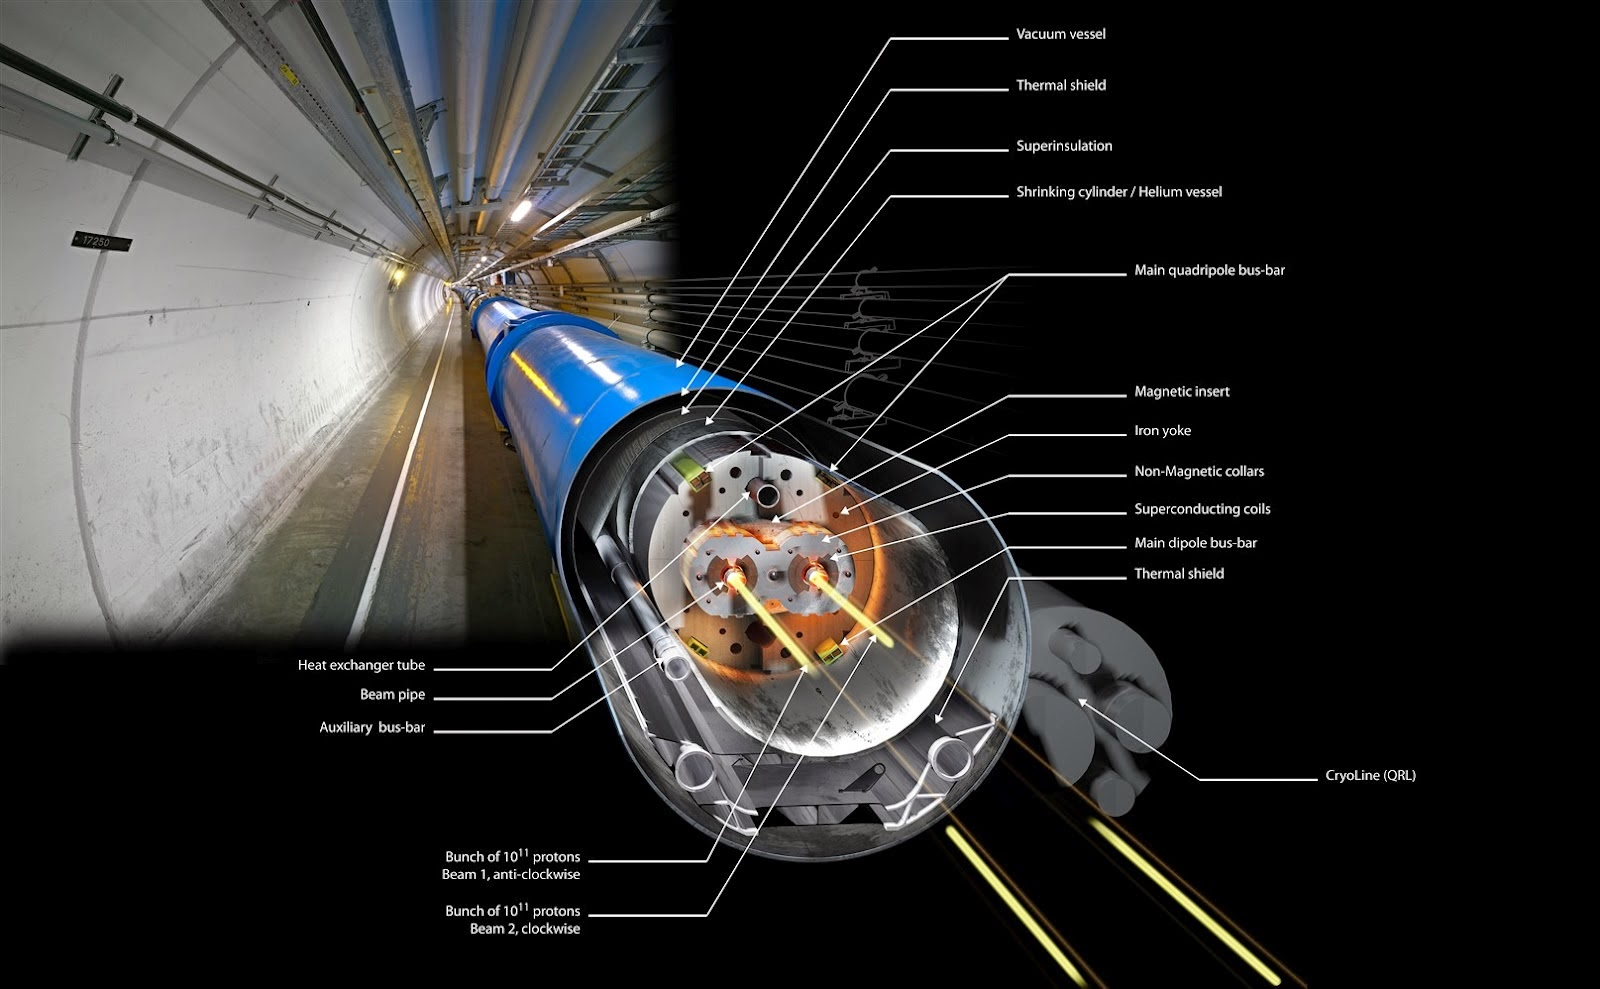
\includegraphics[height=7.5cm,keepaspectratio]{figures/lhc/lhc_dipole_xs.jpg}
    \captionof{figure}
        [Cross section of a dipole magnet at the LHC]
        {A cross section of one of the 1232 dipole magnets which span the entire length of the LHC tunnel.
        Figure taken from~\cite{dipole_xs}.} 
    \label{fig:lhc_dipole_xs}
\end{multiFigure}
%%%%%%%%%%%%%%%%%%%%

% As two bunches (one from the clockwise proton beam and the other from the counterclockwise beam) approach one of the four detector points along the LHC, each bunch is squeezed tightly using quadrupole magnets, helping to focus the beams which increases the chance for the desired \pp collisions.
As the two proton beams approach one of the four detector points along the LHC, two of the oncoming bunches are squeezed tightly by quadrupole magnets which increases the chance for the desired \pp collisions.
During a bunch crossing (BX), amazingly most of the protons just pass right by one another; 
out of the $\approx$$\tentothe{11}$ possible \pp collisions that could have occurred, Fig.~\ref{plt:pileup} shows that on average only approximately 32 collisions occurred per BX during the 2018 Run of the LHC. %, according to a particle detector called CMS, described in Chapter~\ref{ch:cms}.  a mere 50 collisions take place on average (\ie only 0.0001\%).
This is a testament to just how small protons truly are.
% % TODO: Check numbers here and ref.
% There are also 392 quadrupole magnets
% that compress the proton bunches as tightly as possible before collision with the other oncoming proton beam.
%%%%%%%%%%%%%%%%%%%%
\begin{multiFigure}
    \centering
    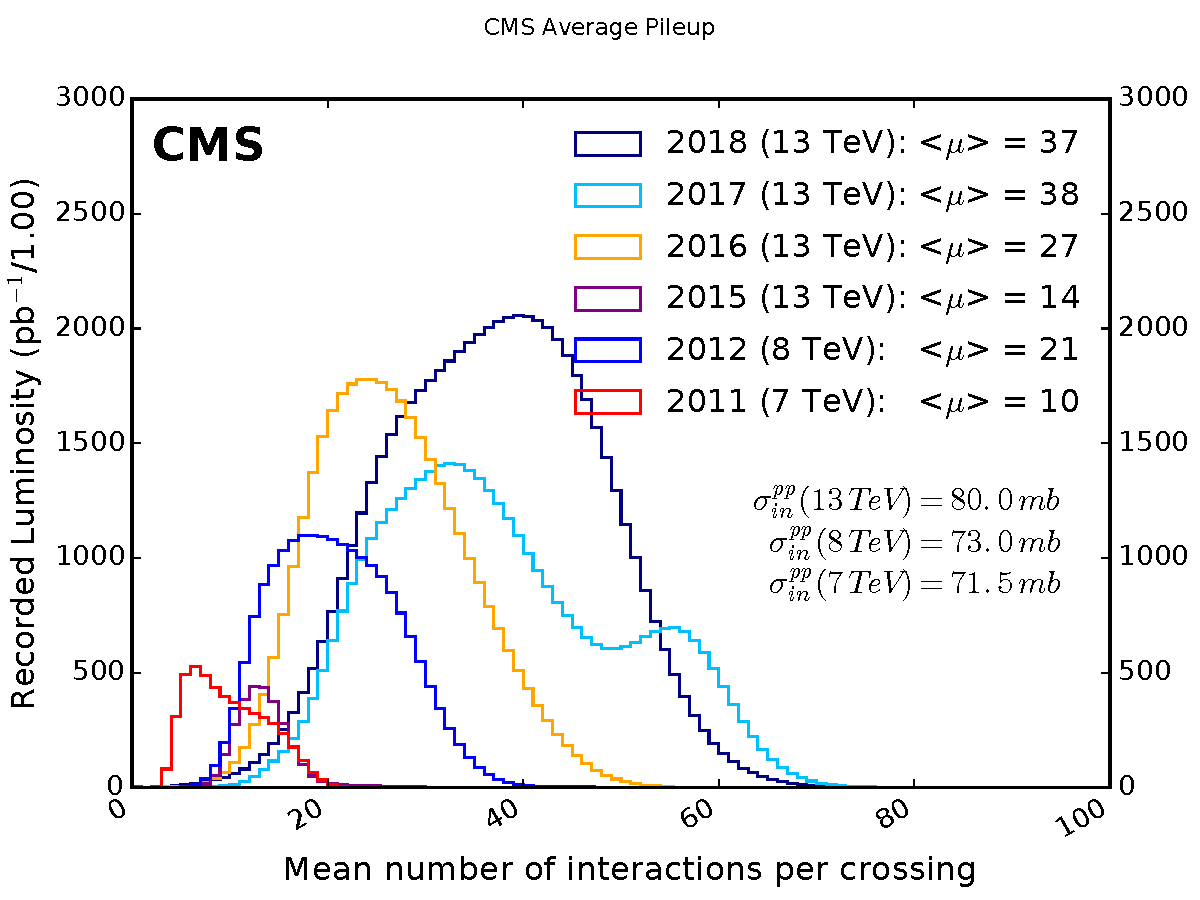
\includegraphics[width=0.85\textwidth,keepaspectratio]{figures/lhc/pileup_allYears.pdf}
    \captionof{figure}
        [Average pileup distribution during various LHC runs]
        {Distributions of the average number of \pp interactions per proton bunch crossing (\emph{pileup}) which CMS recorded during various years over the course of Runs 1 and 2.
        Plot taken from~\cite{pileup}.
        } 
    \label{plt:pileup}
\end{multiFigure}
%%%%%%%%%%%%%%%%%%%%

%from 50 $\mu$m
In the event that \pname does not collide with any of the oncoming protons, then it is simply ``recycled'' and continues going around the LHC ring for another opportunity at a \pp collision.
When the anticipated moment finally comes---\ie a ``hard'' \pp collision is realized, as shown in Fig.~\ref{fig:pp_collision}---the energy of the single collision contains a monstrous center-of-mass energy of \sqrtsthirteen, which is more than enough to create new particles like top quarks, Higgs bosons (Chapter~\ref{ch:higgs_mass}), and potentially BSM particles (Chapter~\ref{ch:dilep_res}).
% Truly, it is the particles inside the protons, the so-called \emph{partons} that interact with one another, as shown in Fig.~\ref{fig:pp_collision}.
In order to analyze such interesting particles, one needs to detect the outgoing particles produced from the \pp collisions.
One such dedicated particle detector is located at Point 5---the Compact Muon Solenoid (CMS) detector---and is described in the next chapter.
%%%%%%%%%%%%%%%%%%%%
\begin{multiFigure}
    \centering
    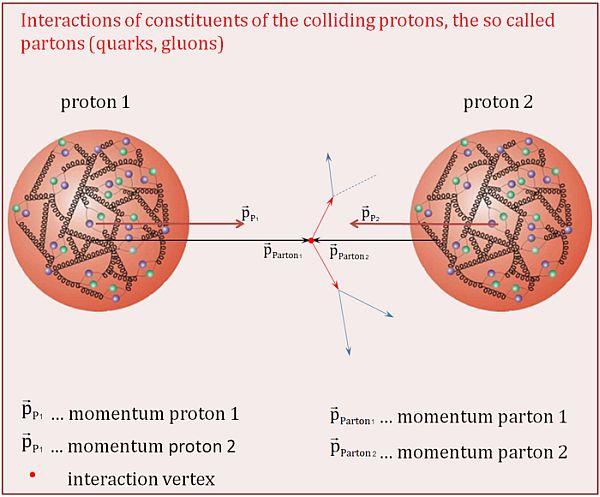
\includegraphics[width=0.8\textwidth]{figures/lhc/proton_proton_quarksandgluons.jpg}
    \captionof{figure}
        [Diagram showing the constituent (\emph{partons}) of two protons interacting in a \pp collision]
        {Two protons can be smashed together at very high energies at the LHC $\left( \sqrtsthirteen \right)$ to have their constituent partons interact and convert into new kinds of matter.
        Figure taken from~\cite{pp_collision}.
        } 
    \label{fig:pp_collision}
\end{multiFigure}
%%%%%%%%%%%%%%%%%%%%
% Finally two incoming proton bunches approach a common collision point.
% - Frequency of BX: considering that proton bunches are spaced 25\ns apart, this means 
% Just as the PS feeds protons into the SPS, which feeds protons into the LHC, so too is it being considered for the LHC to feed a new project---the 100\Km Future Circular Collider.
% LPS SPS
% into a beam pipe going clockwise and another 2800 bunches going around counterclockwise, 
\section{Physics of the LHC}
The merit of a particle collider is typically judged by its center-of-mass energy and a second parameter: the \emph{luminosity}.
In essence, luminosity refers to the `brightness' of the colliding particle beams,
\ie the more tightly packed the particle bunches are, the higher the number of particles per bunch, the more frequently the bunches collide, then the higher the luminosity will be.
Concretely, the instantaneous time-dependent luminosity $(\lumi(t))$ is defined as the ratio between the expected rate $\left( R(t) \right)$ of events and the corresponding cross section $(\sigma)$ for some physics process:
\begin{equation}
    \lumi(t)= \frac{R(t)}{\sigma}.
    \label{eqn:lumi_def}
\end{equation}
Physicists are interested in the total number of events $\left( N^\text{exp} \right)$ they should expect to see in the laboratory---observing a number of events significantly different enough from $N^\text{exp}$ may hint at new physics.
Rearrangement of Eqn.~\ref{eqn:lumi_def} and setting $R(t) = dN^\text{exp} / \dt$ gives the infinitesimal change in the number of expected events after a small increment of time $(\dt)$:
\begin{equation}
    \frac{dN^\text{exp}}{\dt} = \sigma \lumi(t).
    \label{eqn:dNdt}
\end{equation}
Collider experiments typically last over long time periods, so integrating Eqn.~\ref{eqn:dNdt} from some starting time $\left( t_1 \right)$ to some later time $\left( t_2 \right)$, gives $N^\text{exp}$:
\begin{align*}
    N^\text{exp} &= \sigma \int_{t_1}^{t_2}{\lumi(t) \dt}
    \\
    \implies N^\text{exp} &= \sigma \lumiint,
    \label{eqn:Nexp}
\end{align*}
where $\int_{t_1}^{t_2}{\lumi(t) \dt} \equiv \lumiint$ and $\sigma$ is assumed to be independent of time.
% The term $\int_{t_1}^{t_2}{\lumi(t) \dt}$ is the aptly named \emph{integrated luminosity} $\left( \lumiint \right)$ and is a measure of the amount of data collected from $t_1$ to $t_2$.
The term \lumiint is aptly named \emph{integrated luminosity} and is a measure of the amount of data collected from $t_1$ to $t_2$.

When two proton bunches cross at the LHC, the instantaneous luminosity $\left( \lumi_\text{b}\right)$ can be calculated using the so-called \emph{van der Meer method}~\cite{LUM_17_003}:
\begin{equation}
    \lumi_\text{b} = \frac{f_r  n_1  n_2}{A_\text{eff}},
    \label{eqn:lumi}
\end{equation}
where $f_r$ is the LHC frequency of revolution of the particle bunches (11\,245.6\Hz) during collisions,
$n_1$ and $n_2$ are the numbers of particles in each bunch,
and $A_\text{eff}$ is the effective area of overlap between the two bunches.
Since the particle bunches are not infinitely narrow but instead have a cross-sectional profile, $A_\text{eff}$ can be put into terms of the widths of each bunch.
Specifically, if the bunches collide head-on, are Gaussian-distributed, and have the same root-mean-square beam widths ($\sigma_x$ and $\sigma_y$, in the $x$ and $y$ directions, respectively), then Eqn.~\ref{eqn:lumi} becomes:
\begin{equation}
    \lumi_\text{b} = \frac{f_r  n_1  n_2}{4\pi \sigma_x \sigma_y}.
    \label{eqn:lumi_final}
\end{equation}

From Eqn.~\ref{eqn:lumi_final}, it is easy to validate the intuitive description of luminosity as described at the beginning of this section:
$\lumi_\text{b}$ is directly proportional to the numbers of particles in each bunch.
% TODO: Include the below?
% Using the values of the LHC ($f_r = 11\,245.6\Hz$, ) This yields 


% The luminosity of the LHC is $\mathcal{O}(\LHigh)$ the number of particles 
% It should be mentioned that the luminosity of the LHC is on the order of \LHigh. %$10^{34}$ Hz/cm$^2$.

% SPECS
% - Luminosity
% - rates
% - data

% N obs events = xs * eff * Lint 
% cross section is specific to the process
% efficiency is ideally unity.




% The LHC has ushered in the era of ``TeV-scale physics'',
% exploring the 
% - which is about the same amount of energy of a really fat flying mosquito.

% It takes a proton \~90 $\mu$s 
% to make a complete revolution around the LHC moving at such a speed.

% Higgs boson produced every 1 billion collisions.

% Beginning in 2026 (FIXME), the LHC will undergo a ``Phase 2'' upgrade and become the High-Luminosity LHC.
% This upgrade will increase the collider's luminosity by 10 fold (FIXME) and is predicted to deliver SO much data 3000 fb?.

% TODO:
% \section{High-Luminosity LHC}

%%%%%%%%%%%%%
%--- CMS ---%
%%%%%%%%%%%%%
% \chapter{THE CMS DETECTOR} 
\label{ch:cms_detector}
%%%%%%%%%%%%%%%%%%%%
\begin{figure}[pbth]
\centering
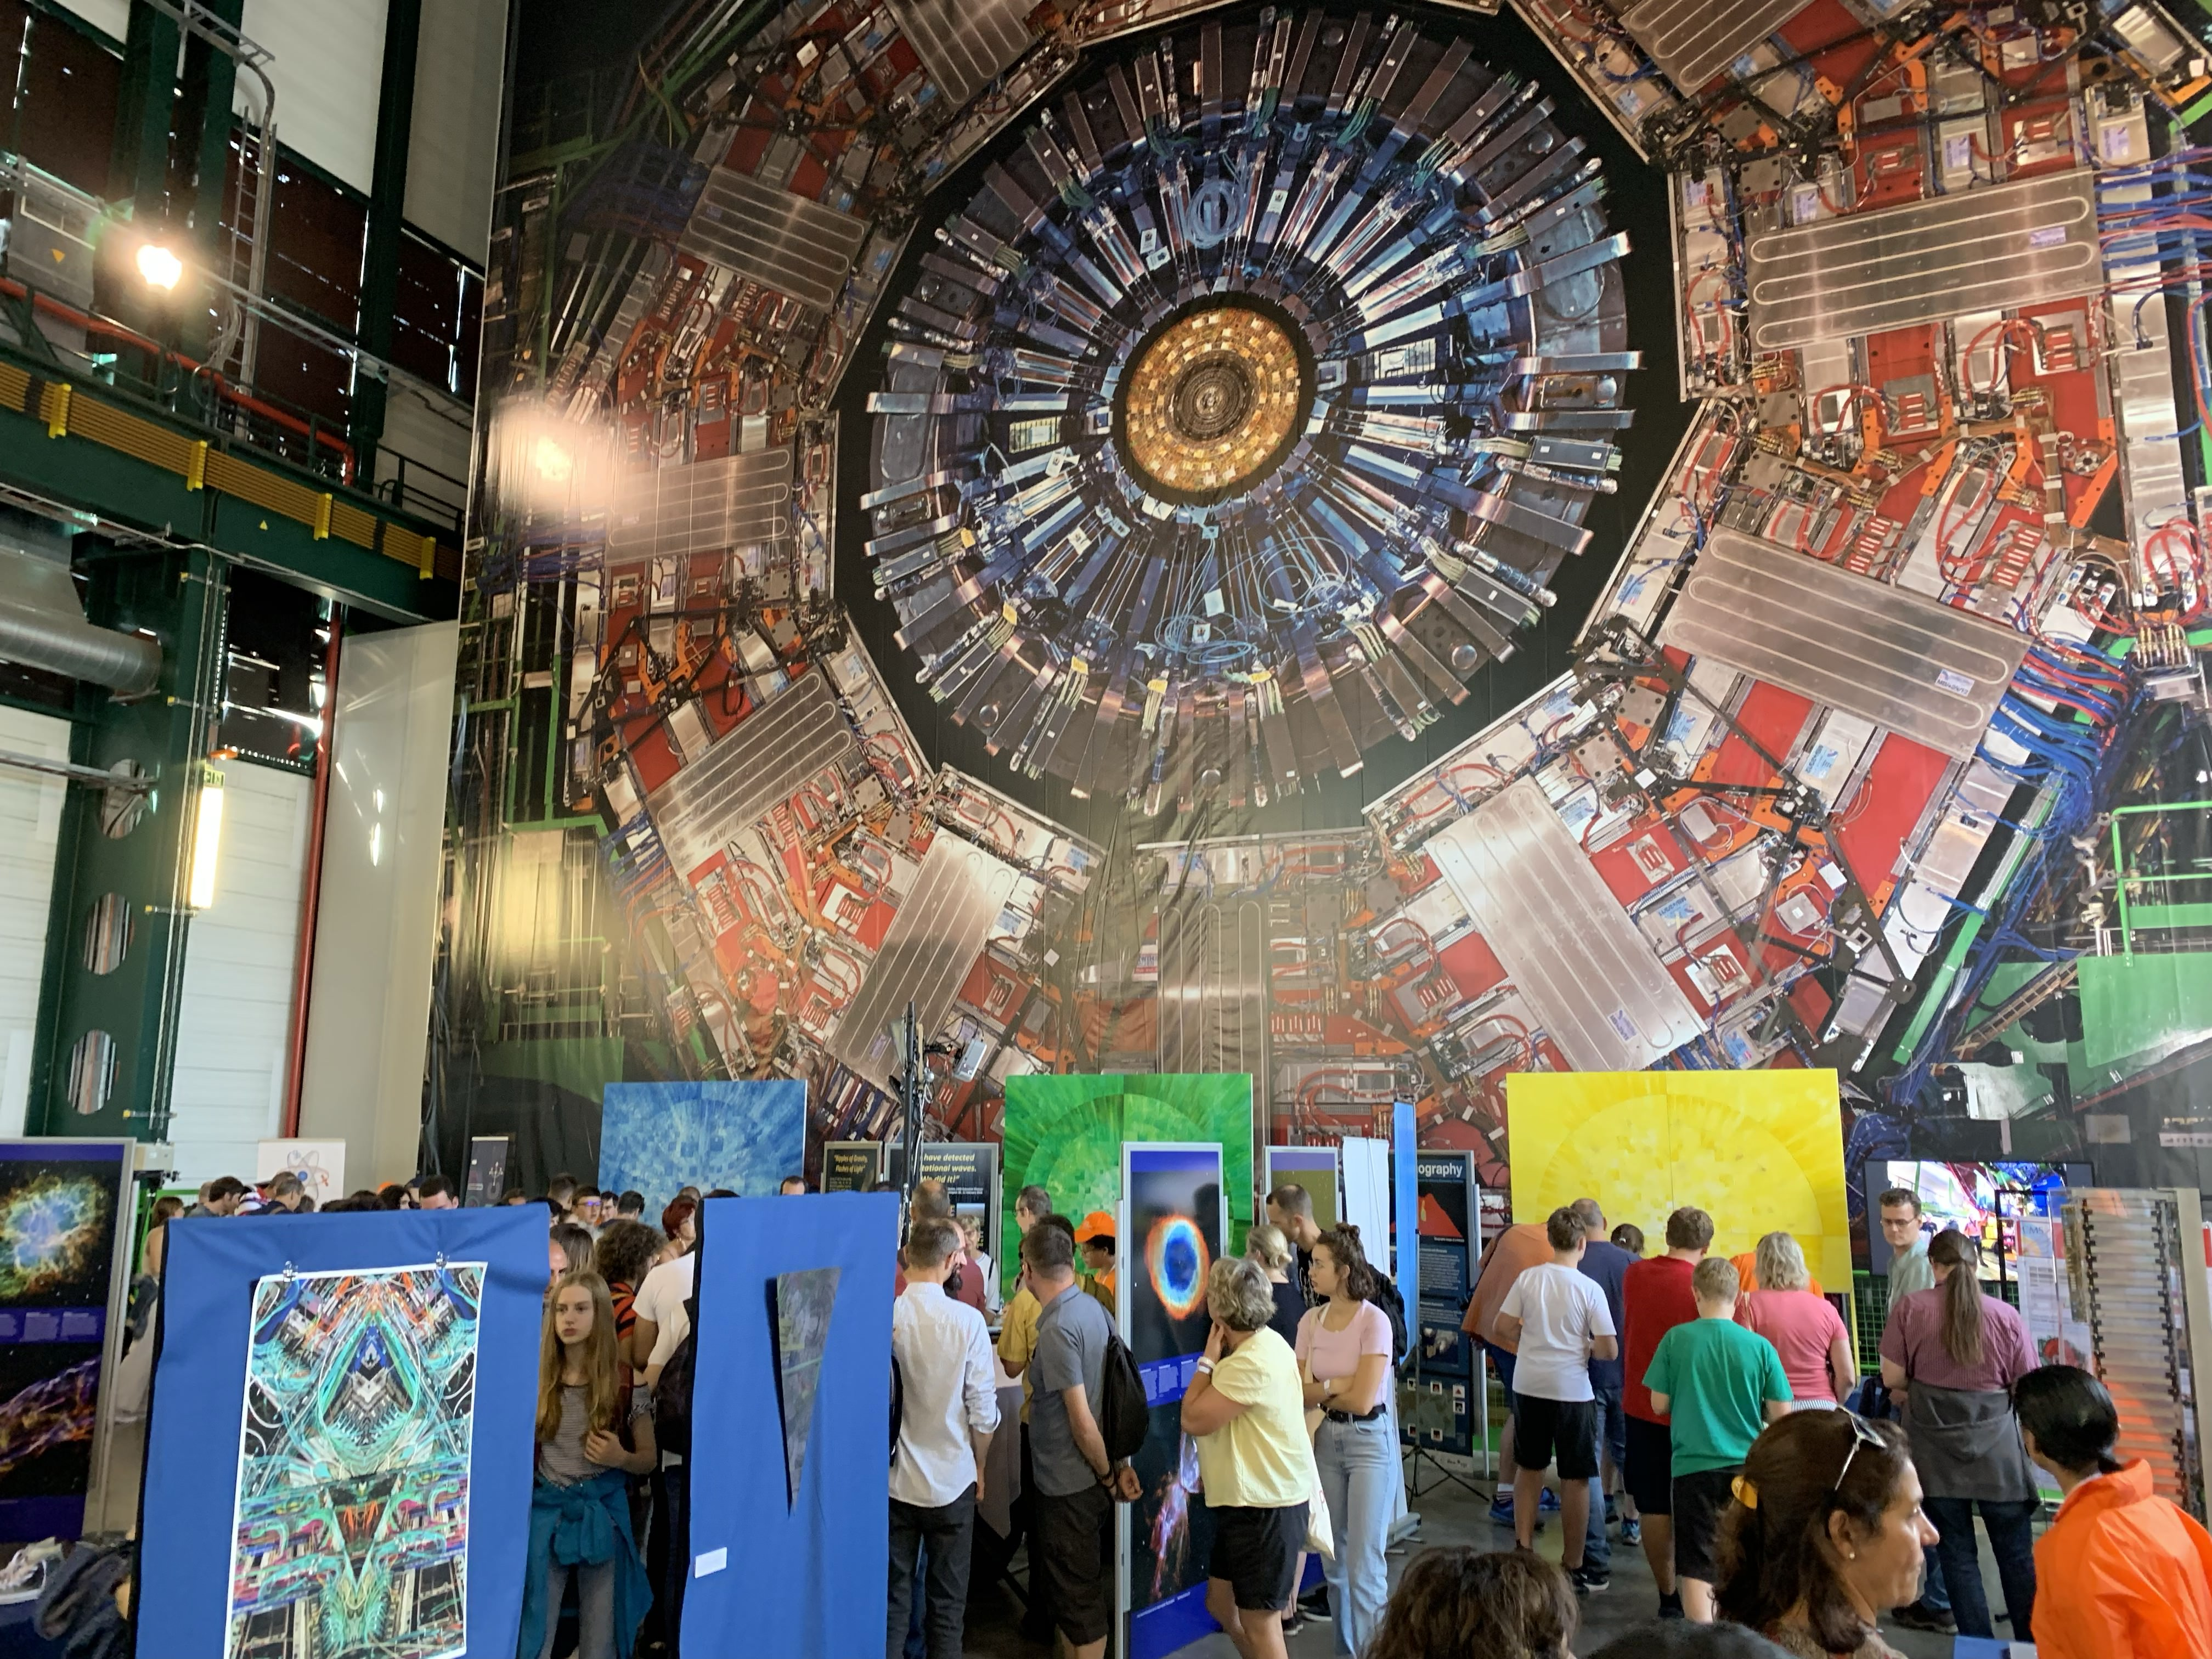
\includegraphics[width=10cm,height=10cm,keepaspectratio]{figures/cms/cms_poster_SX5.jpg}
    \caption{
    Life-size poster of the CMS detector, taken during CERN Open Days 2019
    in the SX5 warehouse where parts of CMS were assembled.}
    \label{fig:cms_poster}
\end{figure}
%%%%%%%%%%%%%%%%%%%%
Weighing in at 14,000 tonnes, standing 5 stories tall (15 m), and reaching 29 m long, the Compact Muon Solenoid (CMS) experiment is one of two general-purpose particle detectors at the LHC (Fig.~\ref{fig:cms_poster}).
CMS is situated approximately 100 m under the earth at the fifth collision point (Point 5) along the LHC (Fig.~\ref{fig:lhc_points}).
In 2012, both CMS and its competing experiment, ATLAS, independently discovered the Higgs boson.

% The purpose of CMS is to precisely measure the kinematical properties of the abundant decay products that come from the \pp collisions delivered by the LHC.
% These particle properties, like momentum, energy, and charge, are used to reconstruct the particle trajectories (``tracks'') and help to identify the particles themselves.
As discussed in Section (TODO: REF), the LHC collides bunches of protons every 25 ns to produce thousands of new particles which then travel away from the interaction point.
CMS is built around the interaction point in a series of cylindrical subdetectors for nearly hermetic coverage so that most of the particles must travel through CMS.
The detector sports a solenoid, after which CMS was named, which generates a 3.8 T uniform magnetic field that points longitudinally down the central axis of CMS.
This strong magnetic field applies a Lorentz force on the outgoing charged particles, causing them to follow helical, momentum-dependent trajectories.
These curved tracks are then better separated from one another which assists in particle identification.
Neutral particles experience no Lorentz force and thus travel in straight lines.

The subdetectors measure the properties of the outgoing particles and carefully filter them out in a clever way (Fig.~\ref{fig:cms_cut_out_view}).
Particles interact with the subdetectors, leaving so called ``hits'' where they passed through.
% As the particles interact with the subdetectors in CMS, they leave leaving indication that 
Hits are reconstructed into tracks.
From the track curvature, deduce charge and momentum of the particles.
Depending on which subdetector (or combination of subdetectors) was hit by the outgoing particles, the type of particle can be deduced.
%%%%%%%%%%%%%%%%%%%%
\begin{figure}[pbth]
\centering
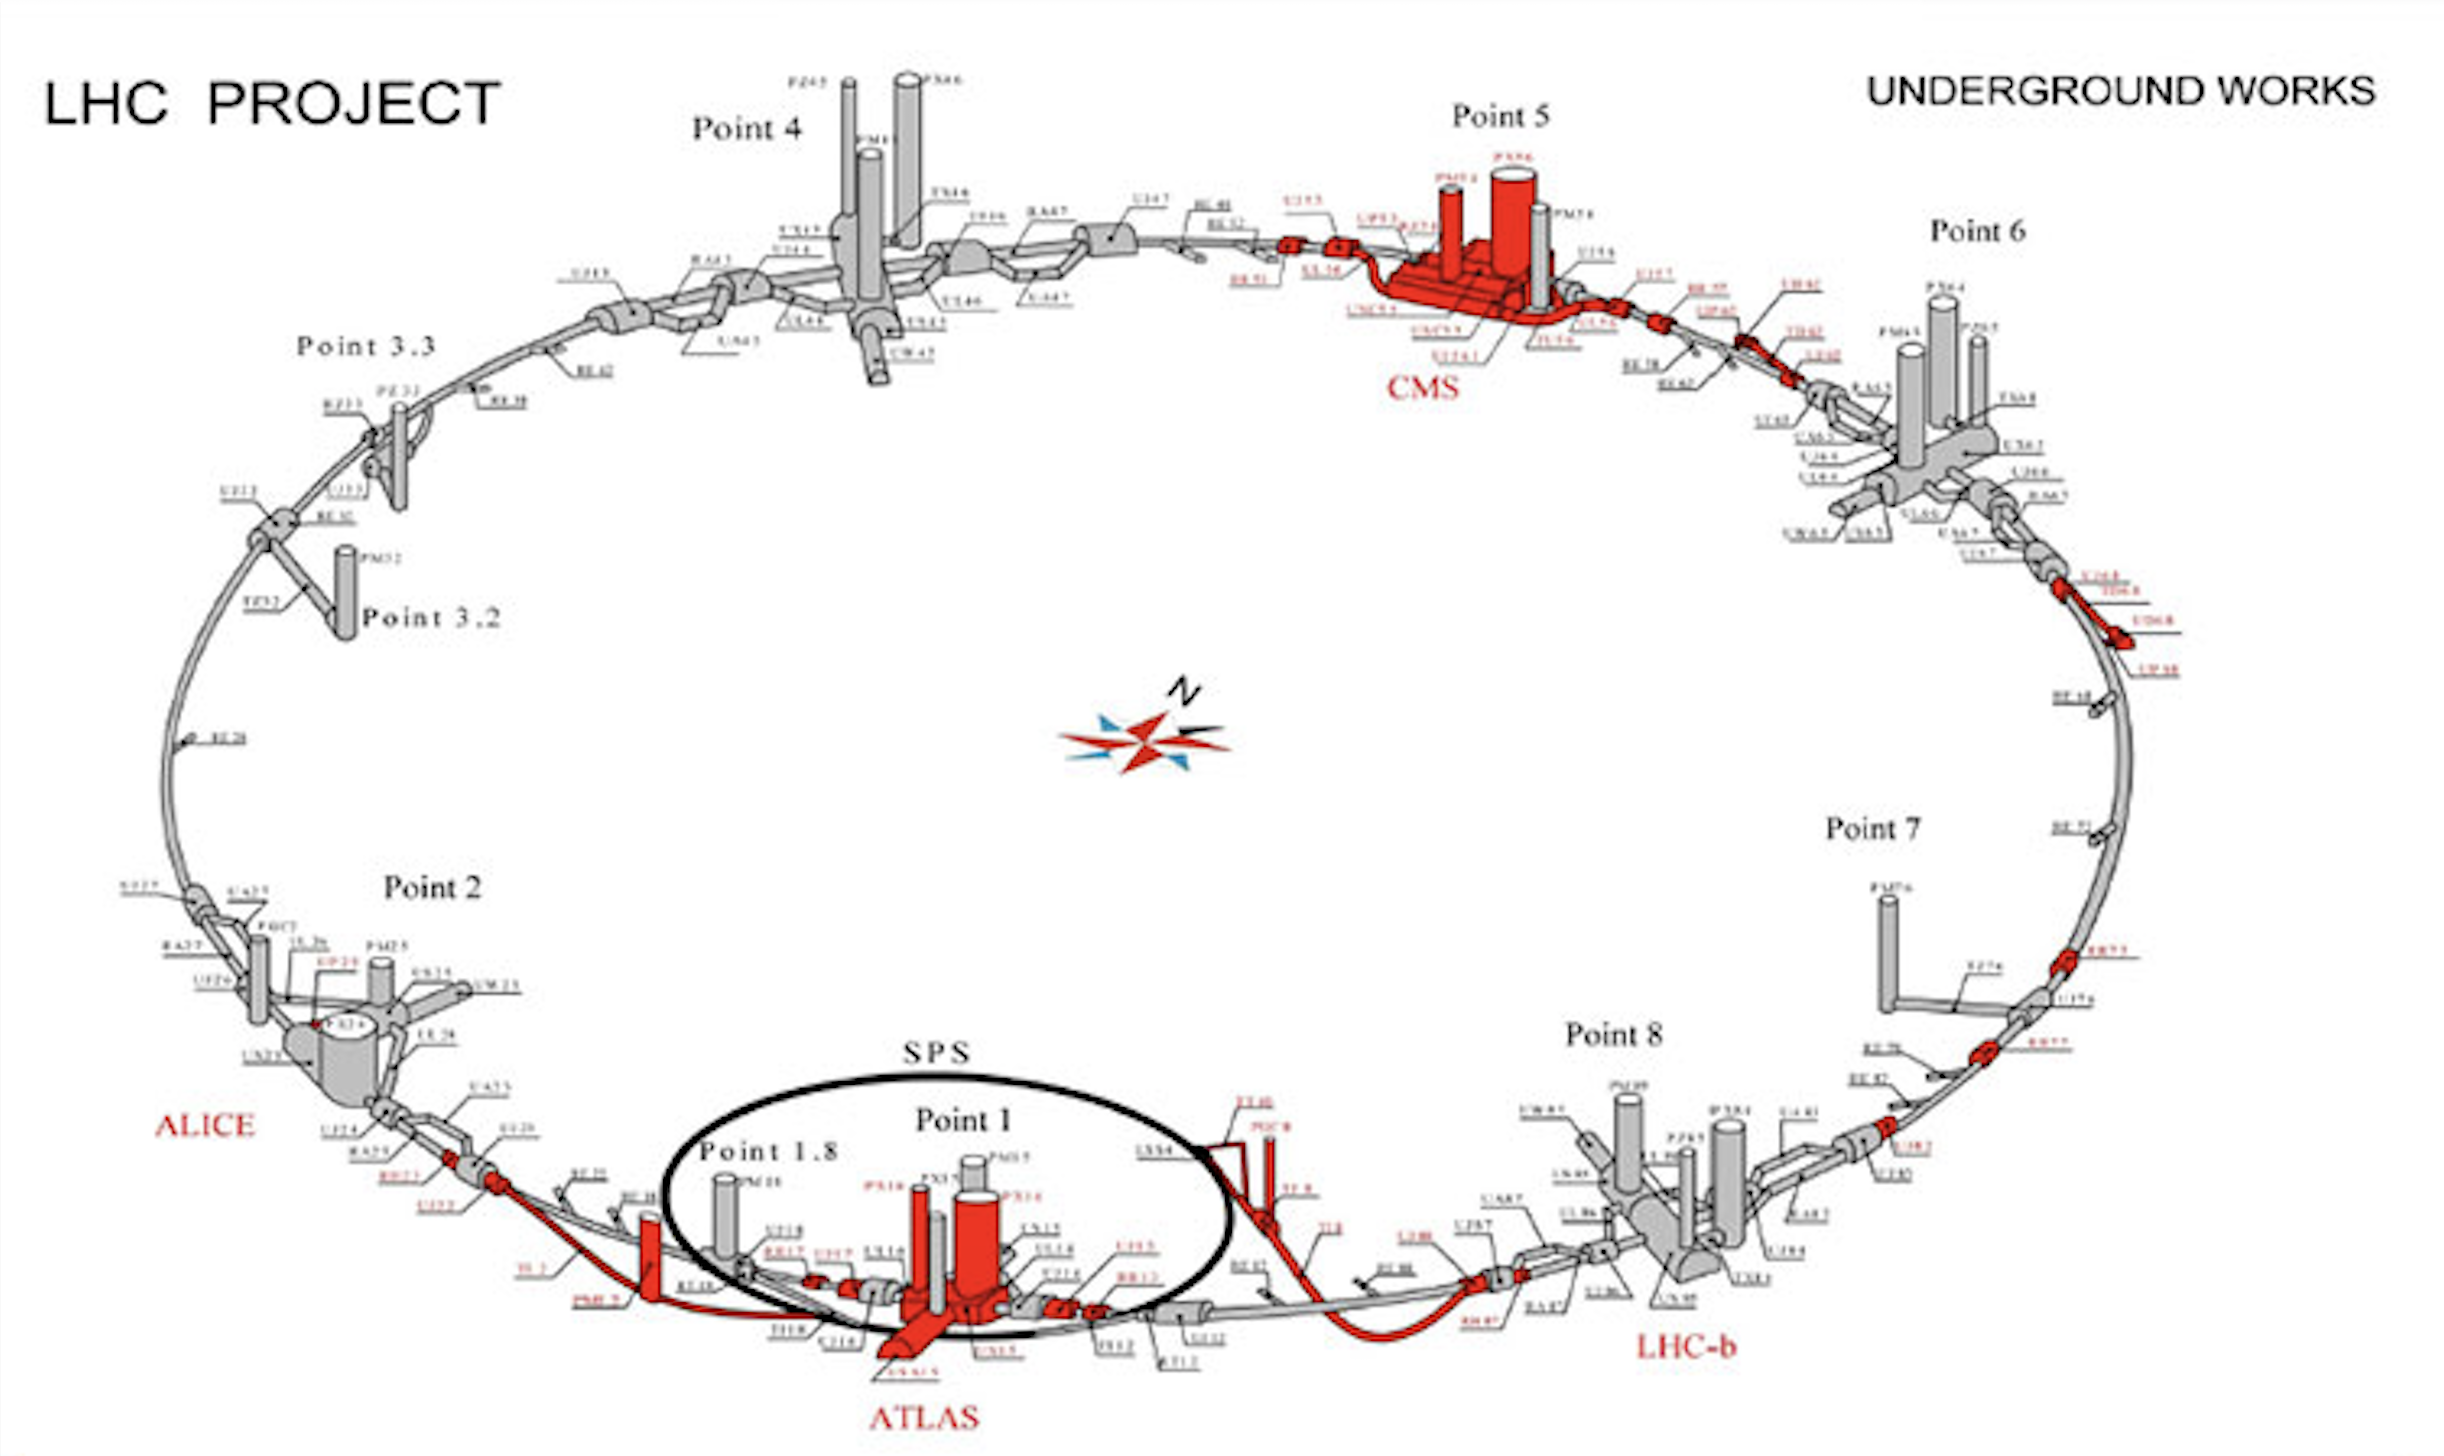
\includegraphics[width=13cm,height=13cm,keepaspectratio]{figures/lhc/lhc_points_with_buildings.png}
    \caption{
    Points 1 through 8 along the LHC.
    Collisions occur at 
    Points 1 (ATLAS), 2 (ALICE), 5 (CMS), and 8 (LHCb),
    whereas the remaining points are used for LHC beam maintenance and testing.} 
    \label{fig:lhc_points}
\end{figure}
%%%%%%%%%%%%%%%%%%%%
%%%%%%%%%%%%%%%%%%%%
\begin{figure}[pbth]
\centering
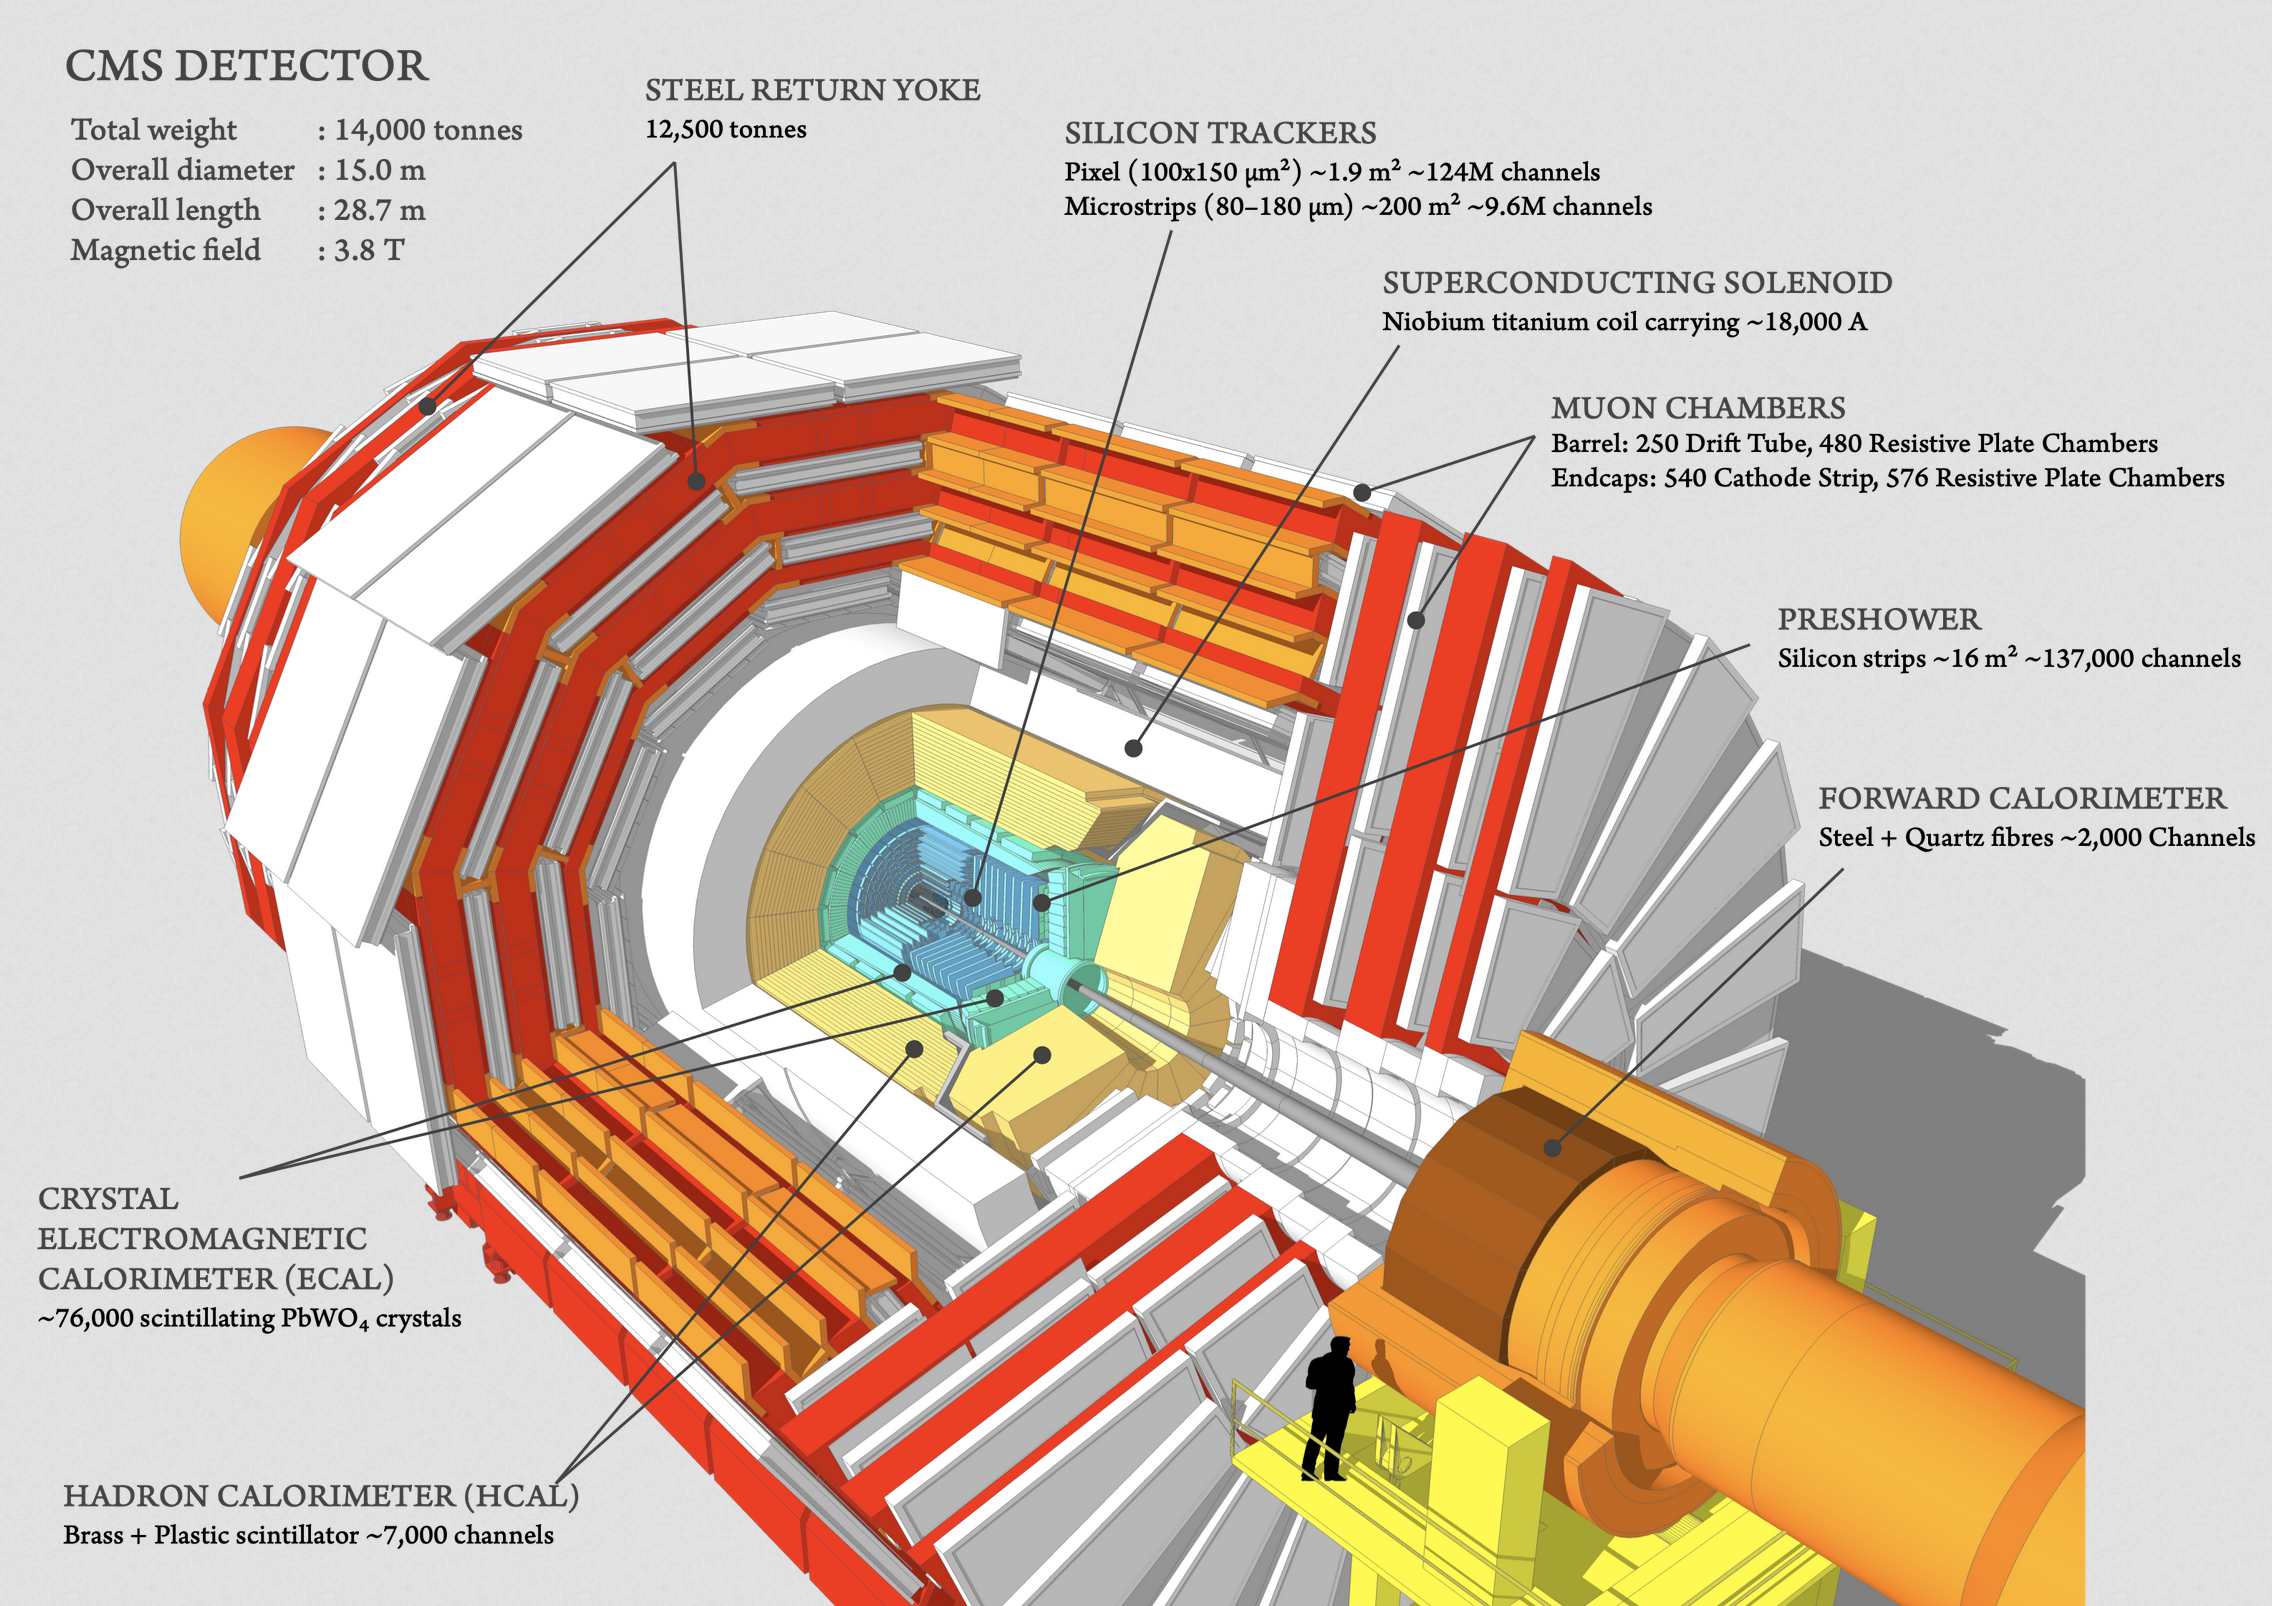
\includegraphics[width=15cm,height=15cm,keepaspectratio]{figures/cms/cms_cut_away.png}
    \caption{Cut out of the CMS detector showing its various subdetector components.} 
    \label{fig:cms_cut_out_view}
\end{figure}
%%%%%%%%%%%%%%%%%%%%
A few example particles and their associated tracks are shown in Fig.~\ref{fig:cms_particle_trajectories}.

Before discussing each subdetector in the following sections, it is useful to define the coordinate system used in CMS:
a typical, right-handed, three-dimensional Cartesian coordinate system $(x, y, z)$ is used, whose center $(0, 0, 0)$ is placed at the nominal \pp collision point within CMS.
The $x$-axis points towards the center of the LHC, the $y$-axis points vertically upward, and the $z$-axis points westward towards the Jura mountains, tangential to the beam direction.
Since CMS covers almost the entire spherical $4\pi$ steradians around the interaction point, it is convenient to use spherical coordinates $(r, \phi, \theta)$,
in which $r$ measures the radial distance in the $x$-$y$ plane, $\phi$ measures the azimuthal angle in the $x$-$y$ plane as measured from the $x$-axis, and $\theta$ measures the polar angle as measured from the $z$-axis.
When dealing with ultra-relativistic particles like those produced at the LHC, special relativistic effects like length contraction must be taken into account and so the coordinate $\theta$ becomes frame-dependent.
It is thus helpful to convert $\theta$ to the Lorentz-invariant quantity called pseudorapidity $(\eta)$,
defined as $\eta = -\ln [ \tan(\theta/2)]$. % Formula comes from: https://twiki.cern.ch/twiki/bin/view/Sandbox/GeorgeAlversonSandbox#Symbols_and_units_natural_units
% \begin{equation*}
%     \eta = -\ln \left(
%         \tan (\theta / 2)
%         \right)
% \end{equation*}
% which surround the 
%%%%%%%%%%%%%%%%%%%%
\begin{figure}[pbth]
\centering
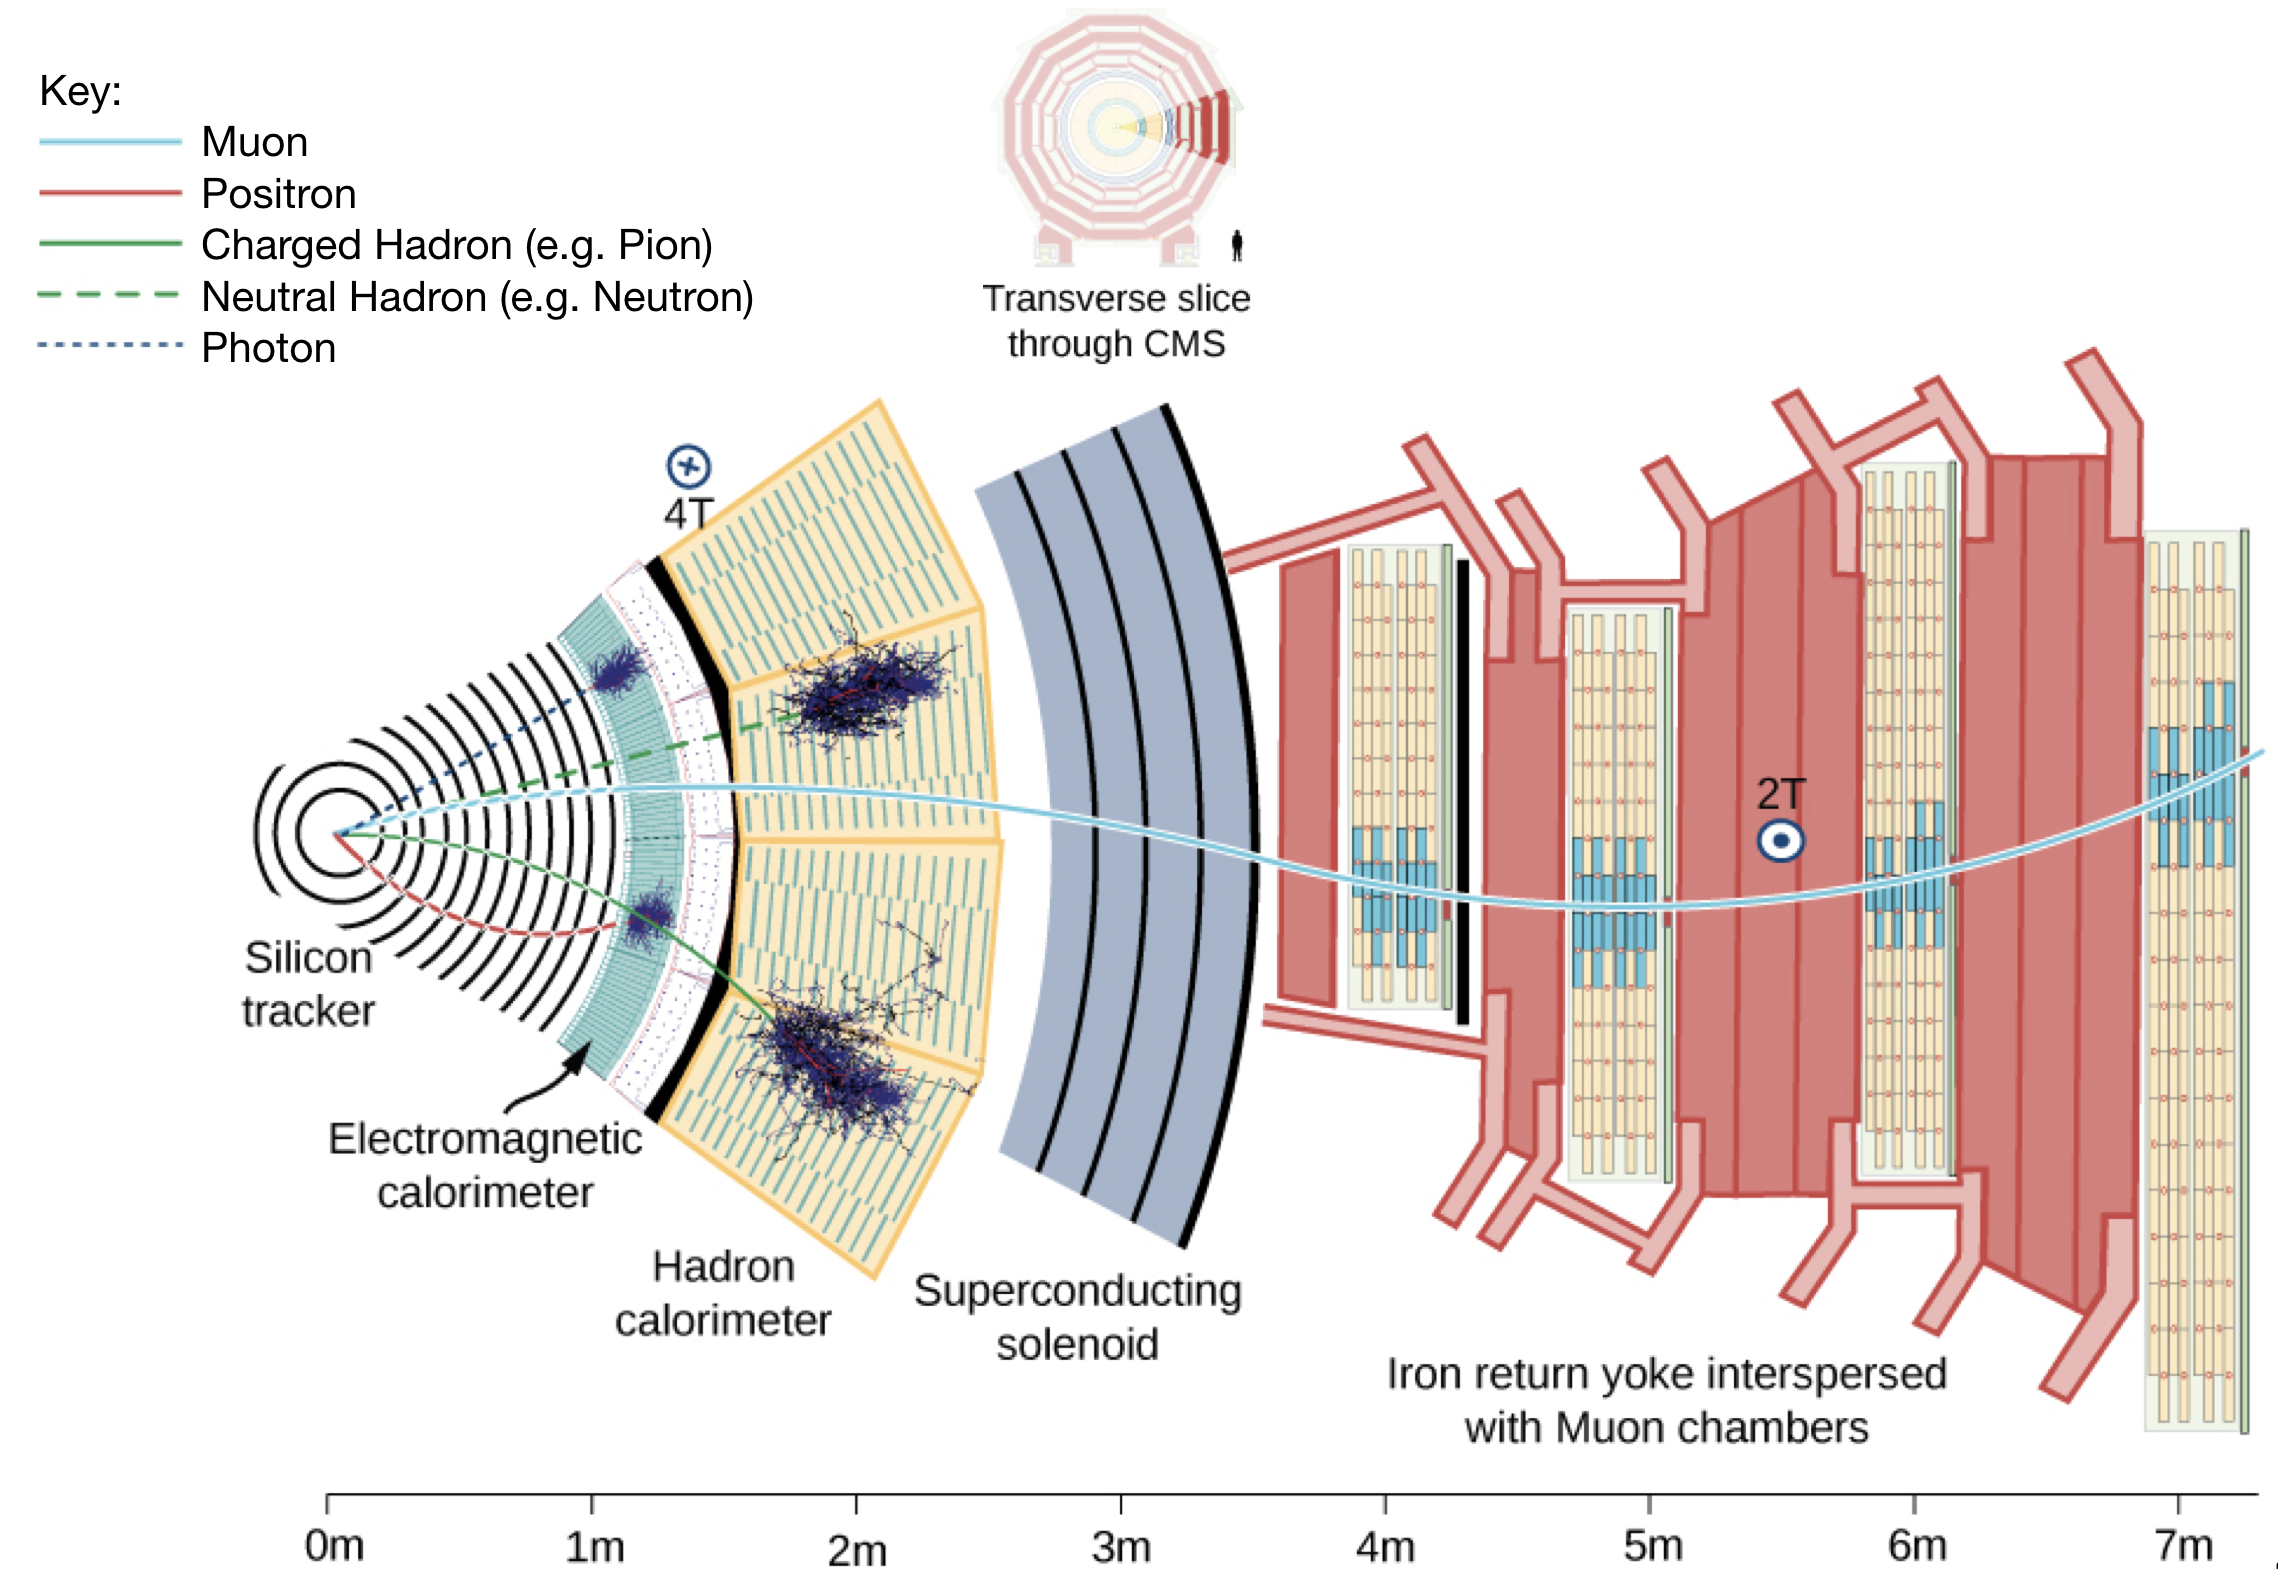
\includegraphics[width=15cm,height=15cm,keepaspectratio]{figures/cms/cms_transverse_particletrajectories_corrected.png}
    \caption{
    A transverse view of CMS showing the ``filtration process'' as different particles pass through different subdetectors.
    A positron (solid red line) curves due to the presence of the magnetic field and gets stopped in the ECAL, creating an EM shower.
    A photon (blue dashed line) does not get detected at all by the Silicon Tracker, since it has no electric charge.
    It continues through to the ECAL and makes a shower here, like the positron.
    Charged hadrons (solid green line) will show curved tracks from the Silicon Tracker, may leave some trace in the ECAL, but primarily get stopped by the HCAL creating hadronic showers.
    Neutral hadrons (dashed green line) do not interact with the tracker, and only undergo EM showers a little in the ECAL, but show most energy deposits in the HCAL.
    Muons (solid blue line) are detected by the Silicon Tracker and then mostly pass through the other subdetectors without interacting until they finally reach the Muon System.
    % In fact you can even determine whether its charge is positive or negative since
    % q v cross B gives the direction of Force.
    % The velocity of the muon is out like this, and the B field is into the screen, so the applied force would be up like this for a positive particle. 
    Using the Lorentz force law and knowing which direction the magnetic field is pointing, one can deduce the sign of the charge of the particle. 
    Based on the radius of curvature from the trajectory, one can then calculate the momentum and energy of the particle.
    % We see that it's not curving up, but curving the other way so we know it must be negative.
    % Notice that since it is curving the opposite way from the muon so we know this is a positive particle.
    % Next up the solid green trajectory represents a charged hadron, like for example maybe an antiproton that got produced.
    % Notice that it would be the same sign as the muon because they curve in the same direction.
    } 
    \label{fig:cms_particle_trajectories}
\end{figure}
%%%%%%%%%%%%%%%%%%%%
% After the protons collide, they make a mess of all sorts of particles:
% electrons, lambda baryons, kaons, muons, photons...
% % TODO: Fix whitespace between word and units.
\section{The Silicon Tracker}
\label{sec:tracker}

At the heart of CMS is one of the world's largest silicon detectors: the silicon tracker.
The main goal of the silicon tracker is not to capture outgoing particles but to very precisely measure the hits from the charged particles as they pass through it.
The tracker also assists in vertex identification, differentiating between primary and secondary vertices, the latter of which often comes from B meson decays.
When multiple \pp collisions occur within the same BX (so-called \emph{pile up}), the tracker distinguishes between proton collisions with a resolution of about 100 \mum longitudinally and 50 \mum transverse to the beam pipe.
This is crucial to resolve which outgoing particles came from which \pp vertex.

The tracker consists of two types of pure silicon detectors: the pixel detector and the strip detector, each of which is described in turn below.
% , and are absolutely necessary to \emph{track} the decay products from \pp collisions.

\subsection{The Pixel Detector}
\label{sec:pixel}

The innermost part of the silicon tracker is the pixel detector, which is the closest subdetector to the interaction point.
The pixel detector is composed of 66 million silicon ``pixels'', as shown in Fig.~\ref{fig:tracker_real} (Left, pink).
A single pixel is 100\mum $\times$ 150\mum and, collectively, they cover a sensitive area of 1.9$\meter^2$.
Because it sits only 8\cm away from the beam pipe, the pixel detector receives the highest particle flux than any other subdetector:
around 10 million particles/$\cm^2$ per second.

The pixel detector is made of three cylindrical layers and two endcaps that surround the beam pipe.
In total, the pixel detector has around 6,000 connections (channels) per$\cm^2$.

After the LHC Run 1 was completed, the accelerator received luminosity upgrades during the 2013--2014 Long Shutdown.
To handle these higher luminosities, the pixel detector was replaced by the CMS Phase-1 pixel detector during the LHC technical stop in 2016--2017.
The upgrades outfitted the detector with four barrel layers and three endcap disks per side, which allowed for particle detection up to $\abseta < 2.5$.
The overall mass of the pixel detector decreased and granted the detector with better tracking capability.

% Cite:
% The CMS Phase-1 pixel detector upgrade
% To cite this article: W. Adam et al 2021 JINST 16 P02027
% https://d1wqtxts1xzle7.cloudfront.net/81437241/Adam_2021_J._Inst._16_P02027-libre.pdf?1645997389=&response-content-disposition=attachment%3B+filename%3DThe_CMS_Phase_1_pixel_detector_upgrade.pdf&Expires=1646800221&Signature=TRRZ5QLjlKL1rSOqgFxAMLY4vgj9EsI-NJSwy3erQAo2jhua1DZakAsJ-q1A4OB6KD1siSA20izwTEhzcojs8hhKZkC0y~gdcmxh7nrKDKmr59F8VMg2xINMemvOxyB9S3-pDxZN9t~VjtHhgAArmHmyLSuu90cy8BAFs3VkyZ1Wbr-RJx2uiRPb2zKXHWQw64laosnzKoBNvFg7B2ZdDaUpryDfPQpyZu3HkwQKV1Jd~ZpXlF0FjvxKm~QTm9Bk~bpxO5G5UiwaNv0sQhnWi37YAvs49yIks0NZrrCP7rbASStJ5L89sgSo44LPZxr3Usm6mGmglhW0eW8HliBYig__&Key-Pair-Id=APKAJLOHF5GGSLRBV4ZA


% REFERENCING THE CMS DETECTOR
% How Hualin has it:
% C. Collaboration, "the CMS Experiment at the CERN LHC," \textit{Journal of Instrumentation}, vol. 3, p. S08004, 2008.
% Compare the above to what gets printed out when you get bibtex working!

\subsection{The Strip Detector}
\label{sec:strip}

The outer part of the silicon tracker is called the strip detector, which has 10 million detector strips spread across 10 cylindrical layers.
The first 4 layers belong to the tracker inner barrel (TIB) and the remaining 6 layers belong to the tracker outer barrel (TOB), Fig.~\ref{fig:tracker_real} (Left, green and blue, respectively). 
Both the TIB and TOB have two endcaps associated with them, the TID and TEC, respectively.
Accounting for all of its components, the strip detector is sensitive to 200$\meter^2$.
Fig.~\ref{fig:tracker_xs} gives a clearly labelled transverse illustration of the pixel and strip detectors.
% It functions similarly to the pixels in that 
% It also has has slightly worse resolution than the pixel detector.
% Both the pixel and strip trackers have barrel and endcap components for nearly hermetic coverage around the beam pipe.
%%%%%%%%%%%%%%%%%%%%
\begin{figure}[pbth]
\centering
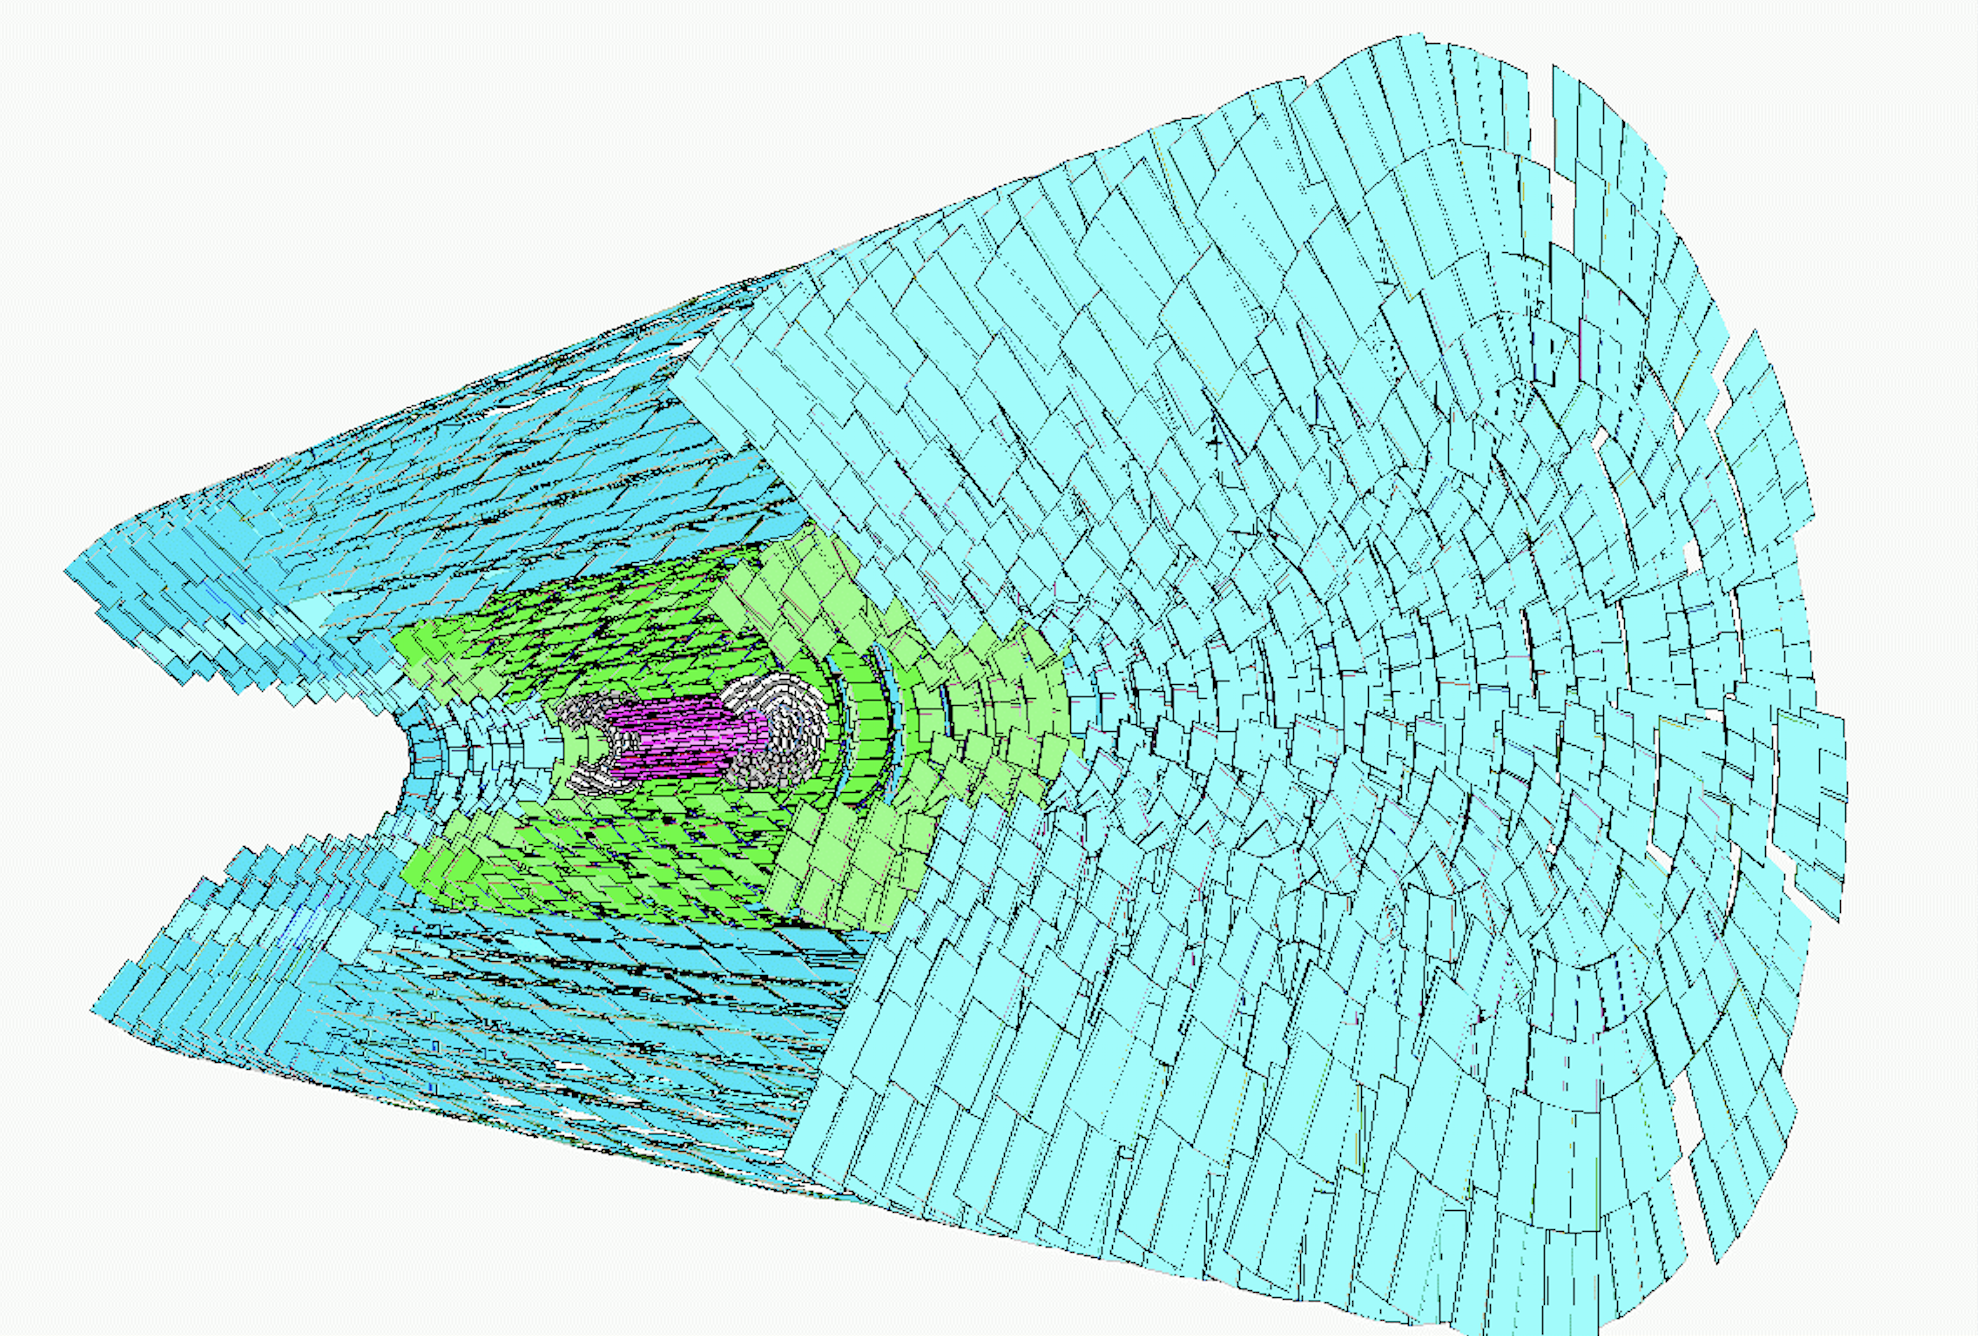
\includegraphics[width=0.49\textwidth,height=10cm,keepaspectratio]{figures/cms/tracker/silicon_tracker_simulated.png}
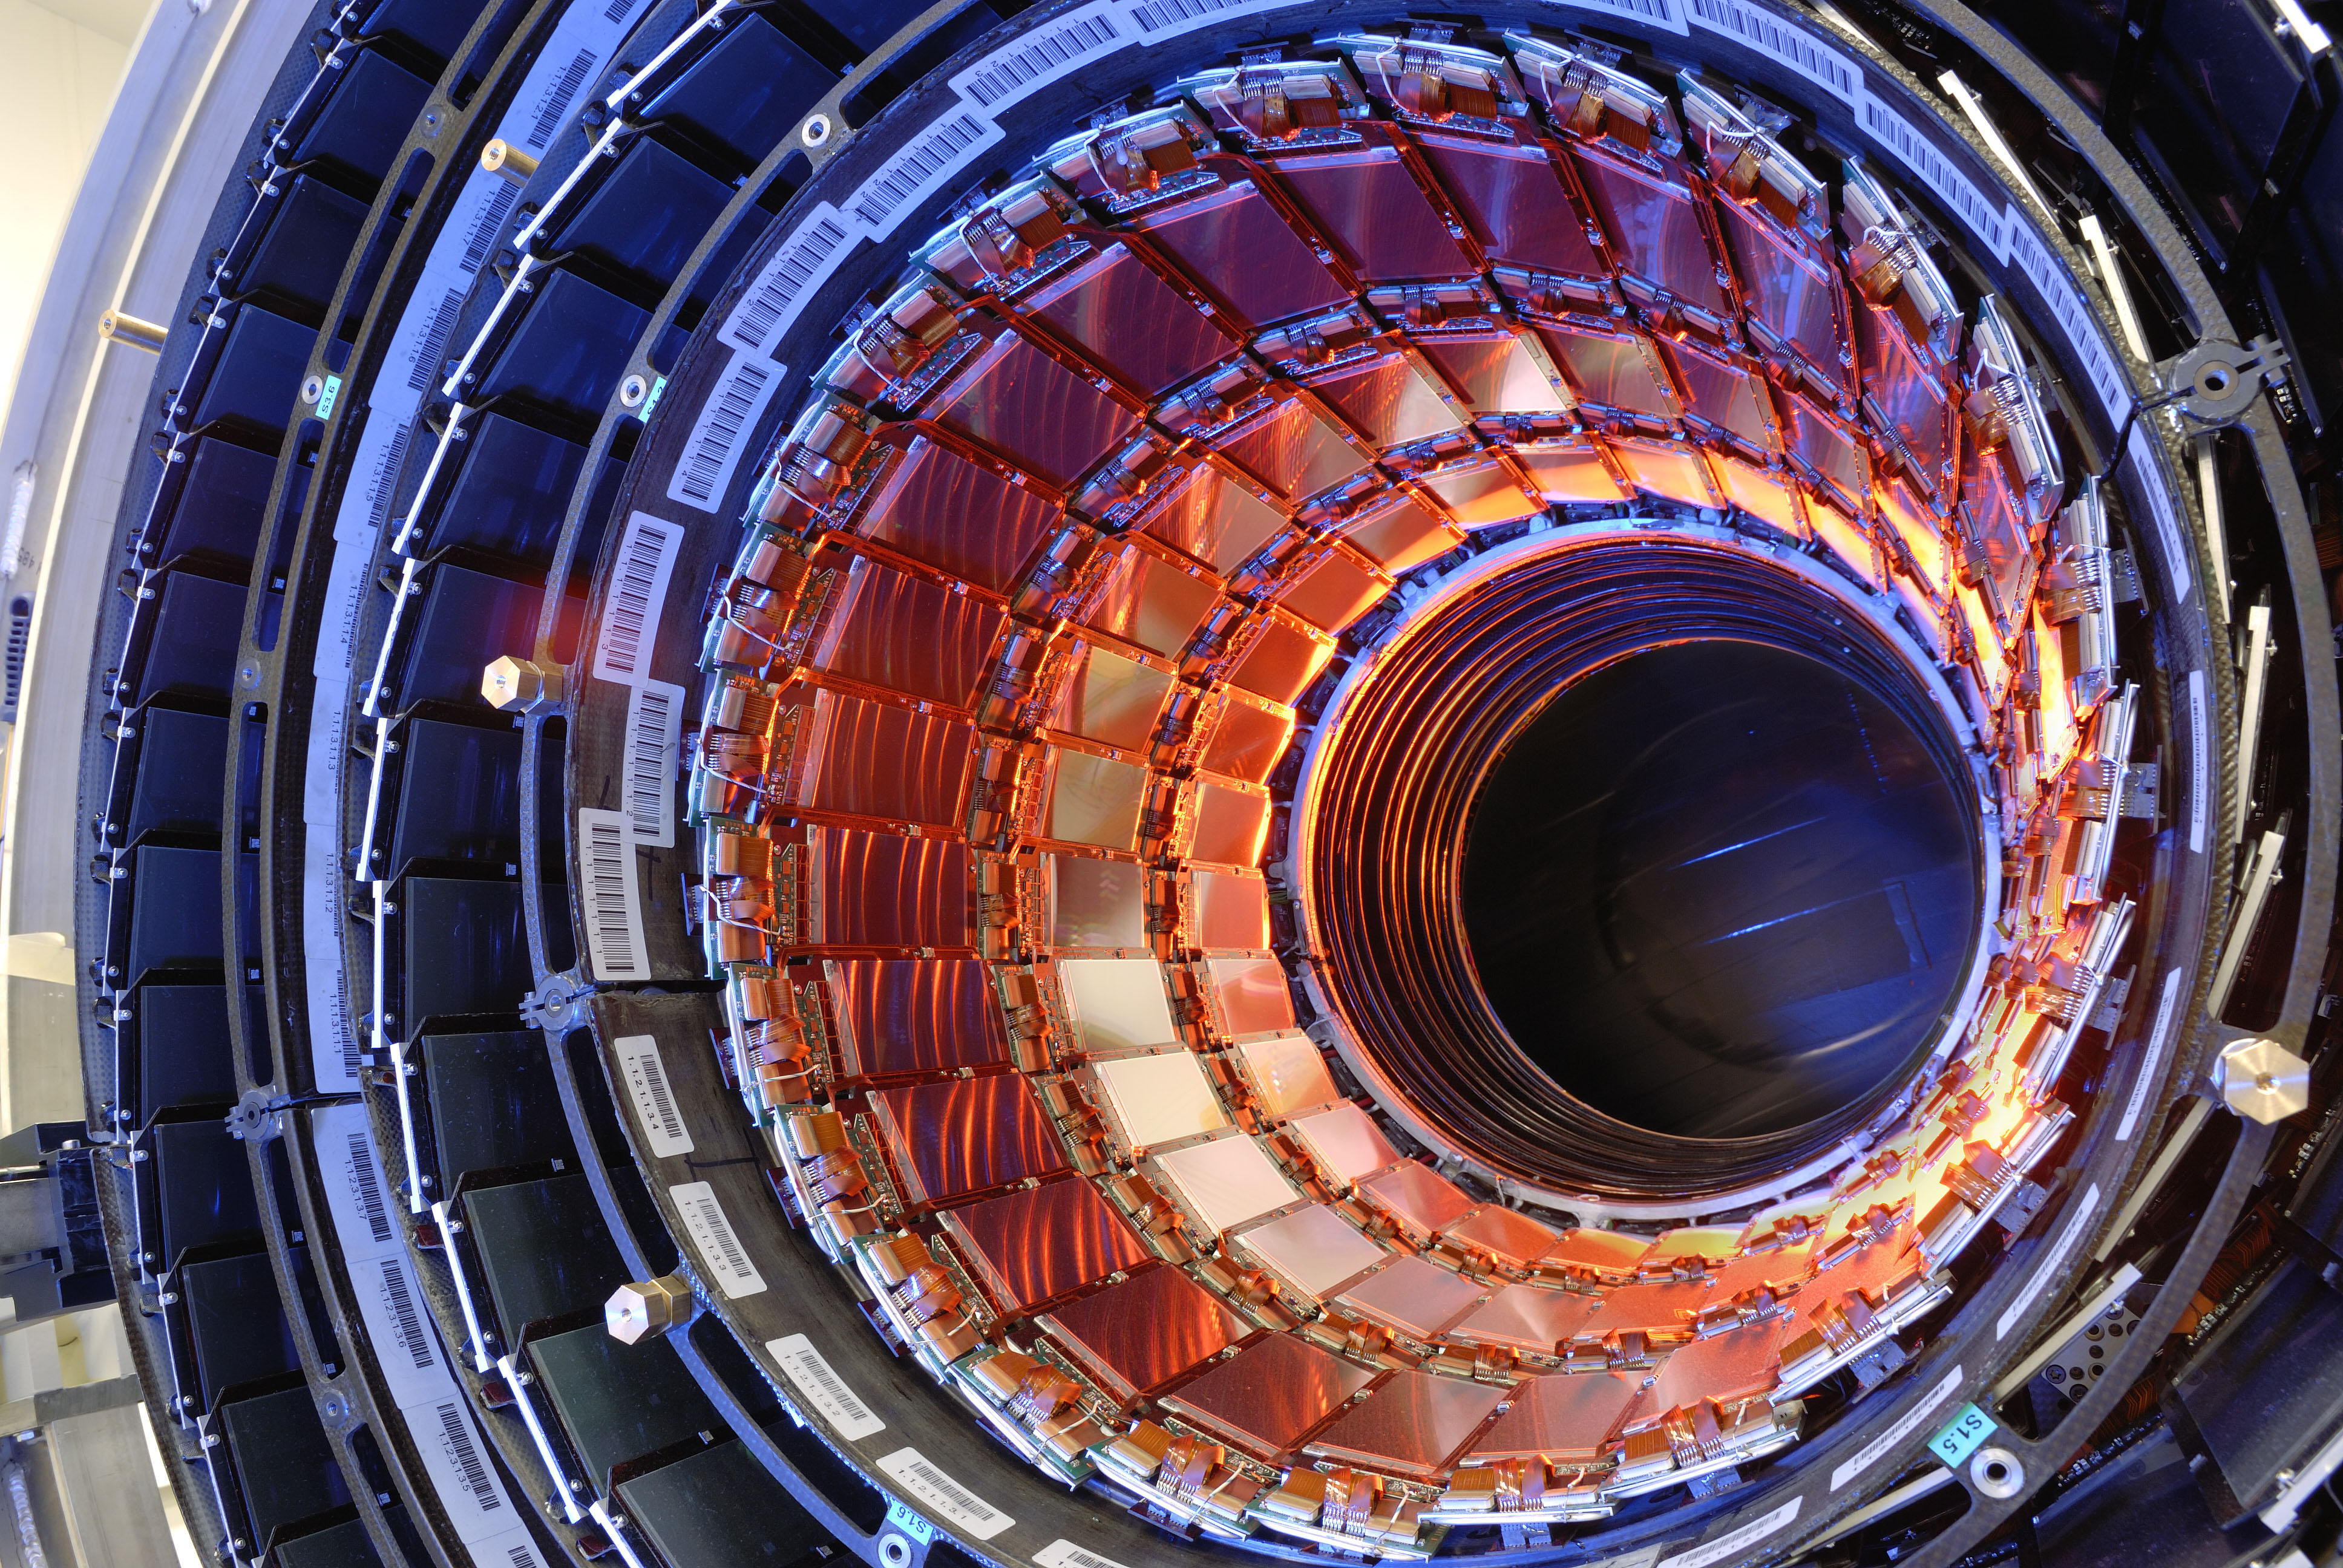
\includegraphics[width=0.49\textwidth,height=10cm,keepaspectratio]{figures/cms/tracker/silicon_tracker_real.jpg}
    \caption
        [(Left) A simulation of the silicon tracker. (Right) The real silicon tracker at the center of CMS]
        {
        (Left) A simulation of the silicon tracker, showing the 3 cylindrical layers of the pixel detector (pink), 4 layers of the TIB (green), and the 6 layers of the TOB (blue) of the strip detector.
        The endcap components are also shown.
        (Right) A picture of the real silicon tracker at the center of CMS.
        } 
    \label{fig:tracker_real}
\end{figure}
%%%%%%%%%%%%%%%%%%%%
\begin{figure}[pbth]
\centering
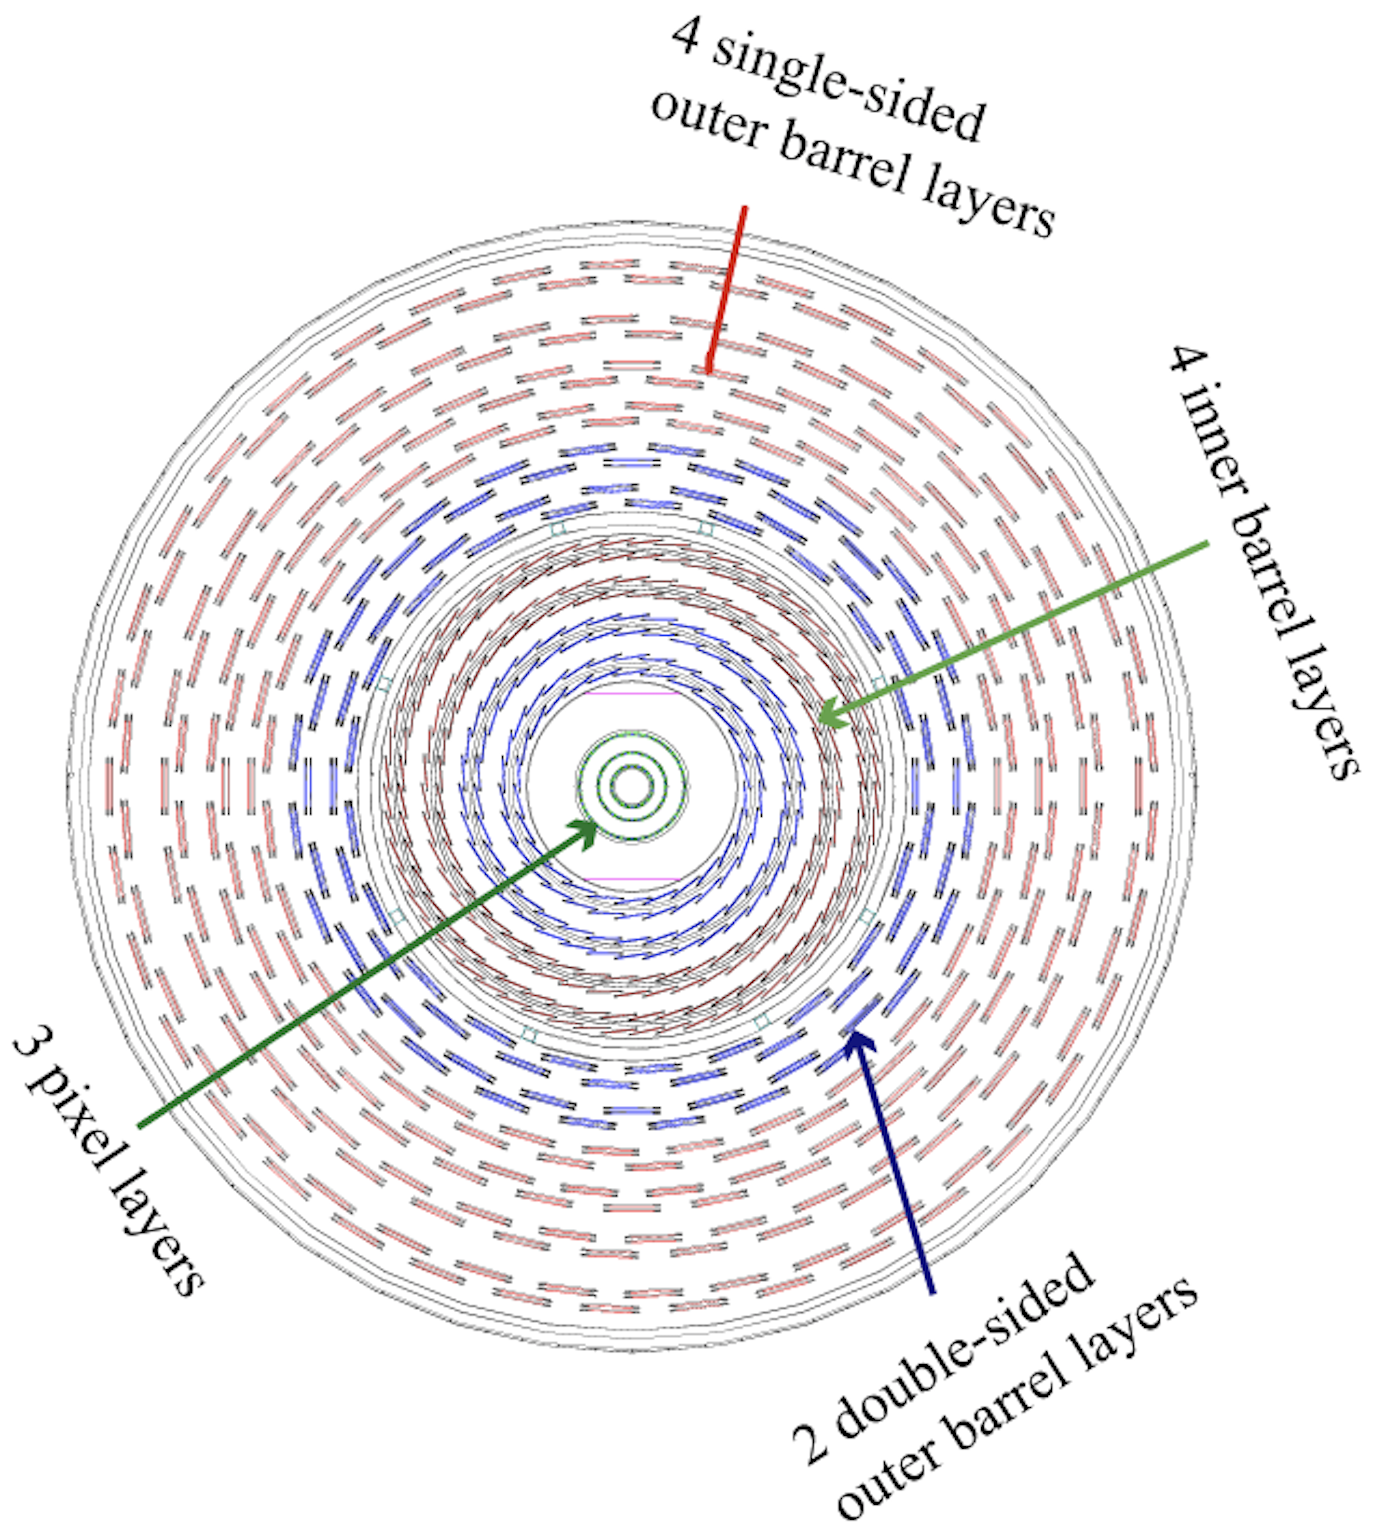
\includegraphics[width=10cm,height=10cm,keepaspectratio]{figures/cms/tracker/silicon_tracker_transverse_view.png}
    \caption{A transverse view of the silicon pixel and strip detectors, explicitly labelling the different layers involved.}
    \label{fig:tracker_xs}
\end{figure}
%%%%%%%%%%%%%%%%%%%%

% Consider the life of a particle produced from a \pp collision:
% Starting at the IP, the produced particles first have an opportunity to interact with the Tracker (Fig.~\ref{fig:tracker_real}, Right).
% Only charged particles will generate ``hits'' in the Silicon Tracker.
% Therefore, photons, neutrons, and neutral pions, \eg, are invisible to the tracker.
% Given enough hits and using sophisticated reconstruction software, we can determine precisely how the particle passed through the tracker.
% It's essentially a fancy game of ``connect-the-dots'' to determine the particle's trajectory.
% Figuring out the trajectory allows one to measure the radius of curvature, and therefore the momentum of the particle.
% This is what makes the Silicon Tracker such an important subdetector.

% Another major benefit of the Silicon Tracker is its assistance in vertex identification.
% During pile up (multiple proton collisions happening within the same BX),
% the tracker distinguishes between proton collisions with a resolution of about 
% 100~\mum longitudinally and 50~\mum transverse to the beam pipe.
% This is crucial to resolve which outgoing particles came from which \pp vertex.
% Since the tracker wasn't built to catch particles, they usually continue on to the next subsystems.
% Thus, CMS must be built as a kind of ``particle filter''.
% Electrons and photons are the first to be filtered out by the Electromagnetic Calorimeter...

% \section{The Calorimeters}
\label{sec:calo}

\subsection{Electromagnetic Calorimeter}
\label{subsec:ecal}

% WHAT IT IS
\textit{\textbf{What is it?}}
Particles that pass through the silicon tracker~\ref{sec:tracker} encounter the electromagnetic calorimeter (ECAL).
Those particles which interact electromagnetically but not strongly, mostly photons and electrons, are typically absorbed by the ECAL.
The particle's energy is then transferred to the ECAL in the form of an electromagnetic (EM) shower.
The size and shape of the EM shower provide information about the particle's energy and trajectory.
Since the Higgs boson can decay into two photons, it was essential that the ECAL was able to detect this decay mode.

% STRUCTURE
\textit{\textbf{Structure:}}
The ECAL is a hermetic, cylindrical, homogeneous sub-detector that consists of a barrel (EB), two endcaps (EE), and a preshower detector in front of each endcap (Figure~\ref{fig:ecal_xs}, Left).
The EB covers $\abseta < 1.479$ while the EE covers $1.479 < \abseta < 3.0$.
The entire subdetector is composed of transparent lead tungstate (PbWO$_4$) crystals that point axially towards the center of CMS (the interaction point).
The transparent crystals, one of which is shown in Fig.~\ref{fig:ecal_crystals} (Left), have a high density (8.28 g/$\cm^3$) which provides the ECAL with radiation resistance and a short radiation length ($X_0 = 0.89~\cm$).
Because so many crystals are used (61,200 crystals in the EB and 7,324 in the EE), the ECAL has excellent energy resolution and fine granularity.
Each endcap is composed of two ``Dee''s, one of which is shown in Figure~\ref{fig:ecal_xs} (Right).
A single Dee carries 3,662 crystals.
Crystals in the barrel are tapered, having front face dimensions $2.2 \times 2.2~\cm^2$, back face dimensions $2.6 \times 2.6~\cm^2$, and are 23.0 \cm long (25.8 $X_0$).
Crystals in the endcaps are also tapered, with front face dimensions $2.862 \times 2.862~\cm^2$, back face dimensions $3.0 \times 3.0~\cm^2$, and are 22.0 \cm long (24.7 $X_0$).
This gives a single crystal from the barrel a volume of approximately 132.5 $\cm^3$ (mL), about the volume of a small cup of coffee, yet it weighs 1.5 Kg.
(REF:PDG).
REF:PDG
Particle Data Group collaboration, S. Eidelman \etal., \textit{Review of particle physics},
\textit{Phys. Lett. \textbf{B 592 (2004) 1}}

% ECAL diagram
\begin{figure*}[!htb]
    \centering
    \captionsetup{justification=justified}
    % 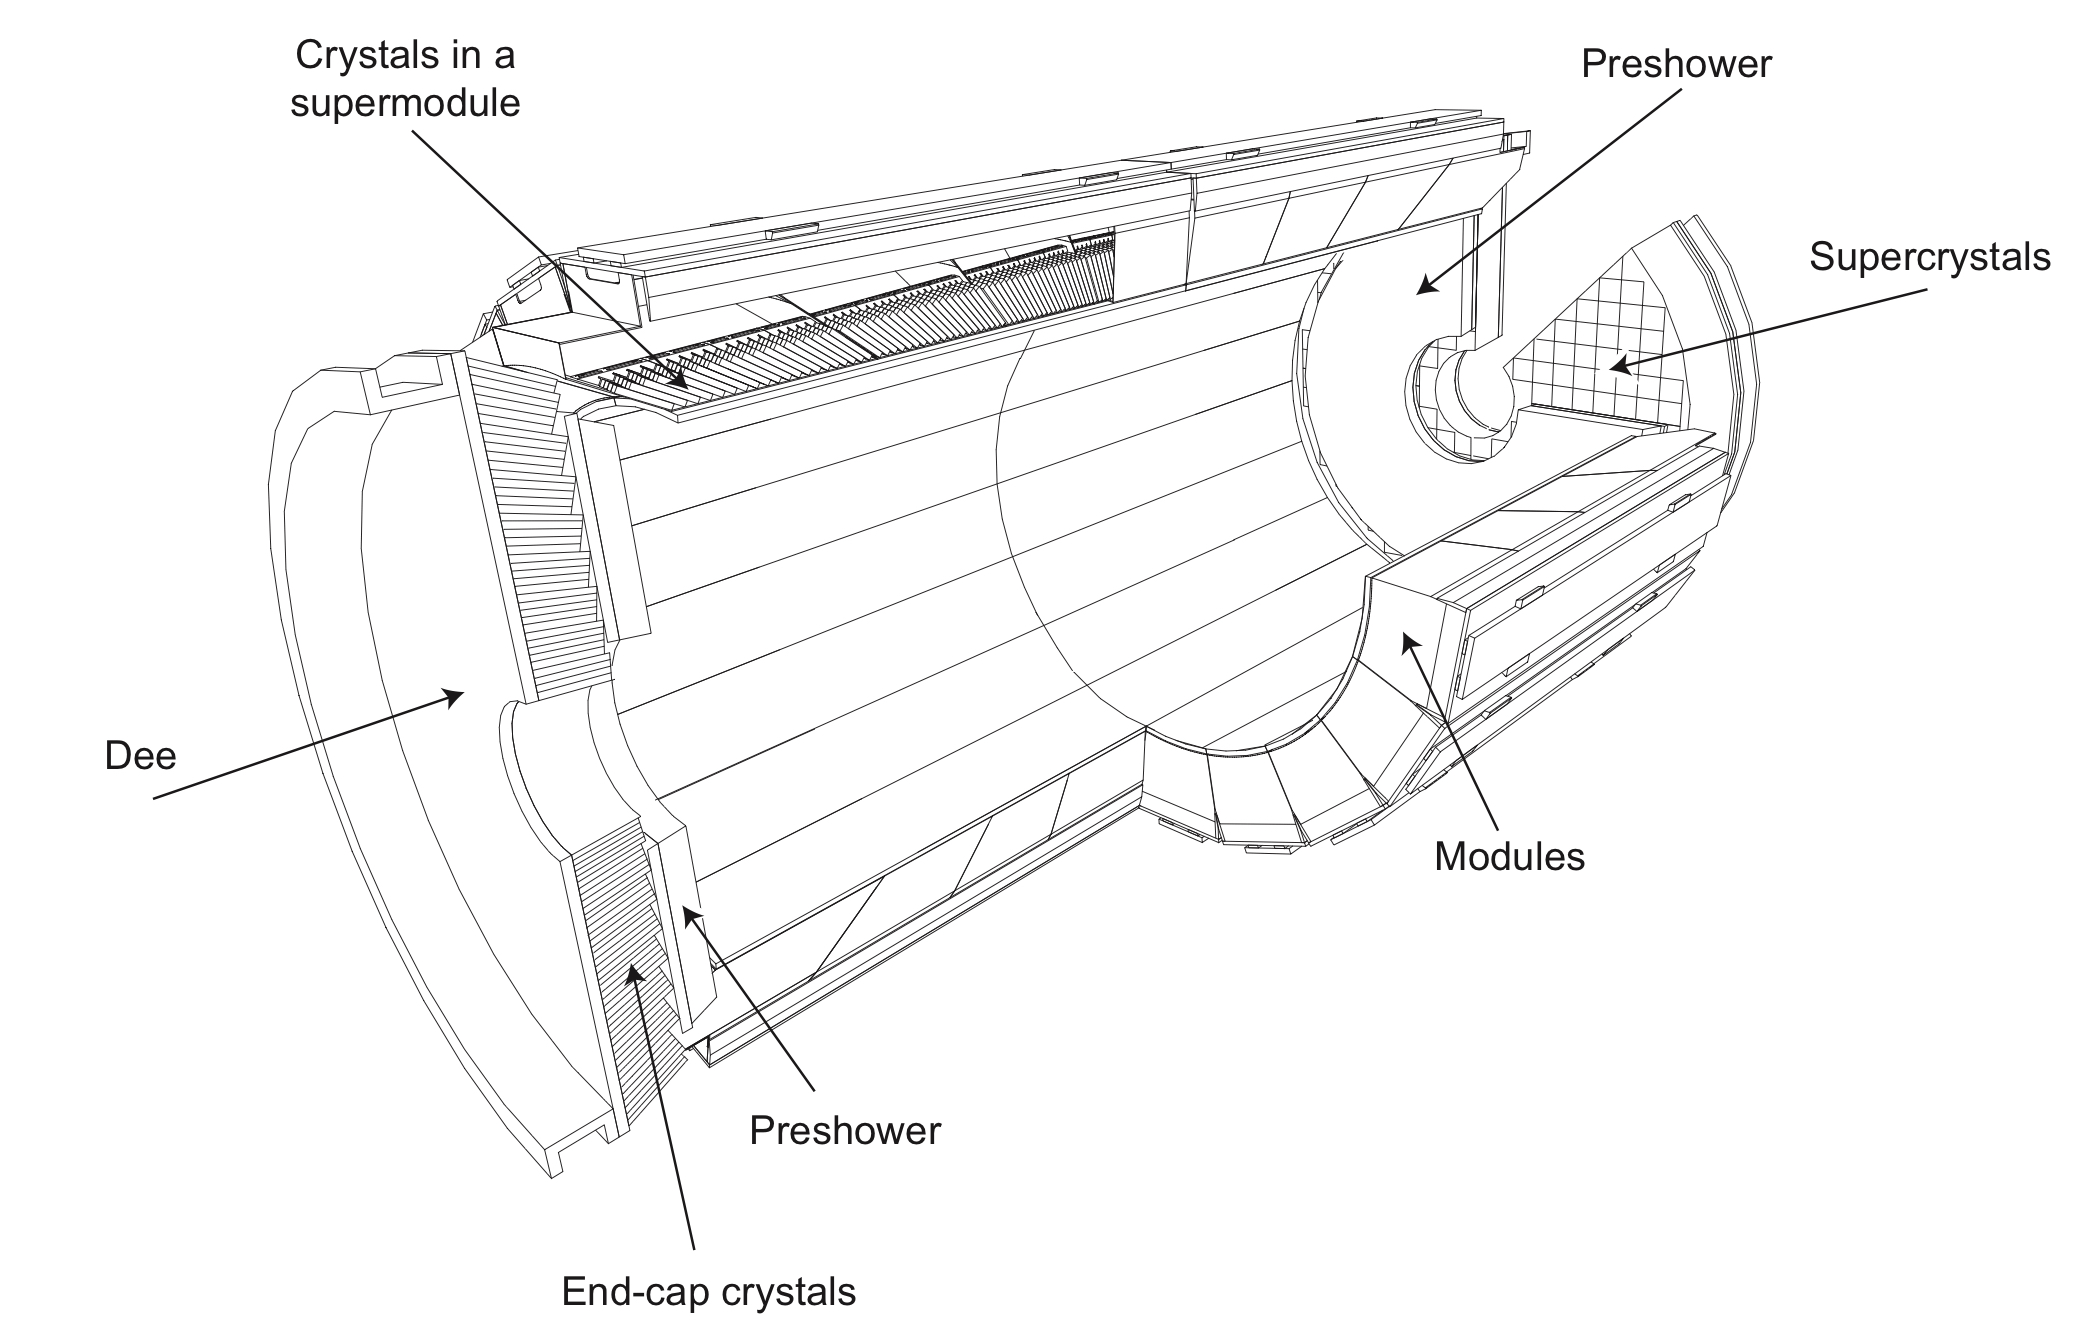
\includegraphics[width=0.95\textwidth]{figures/cms/ecal/xs_whiteblack.jpeg}
    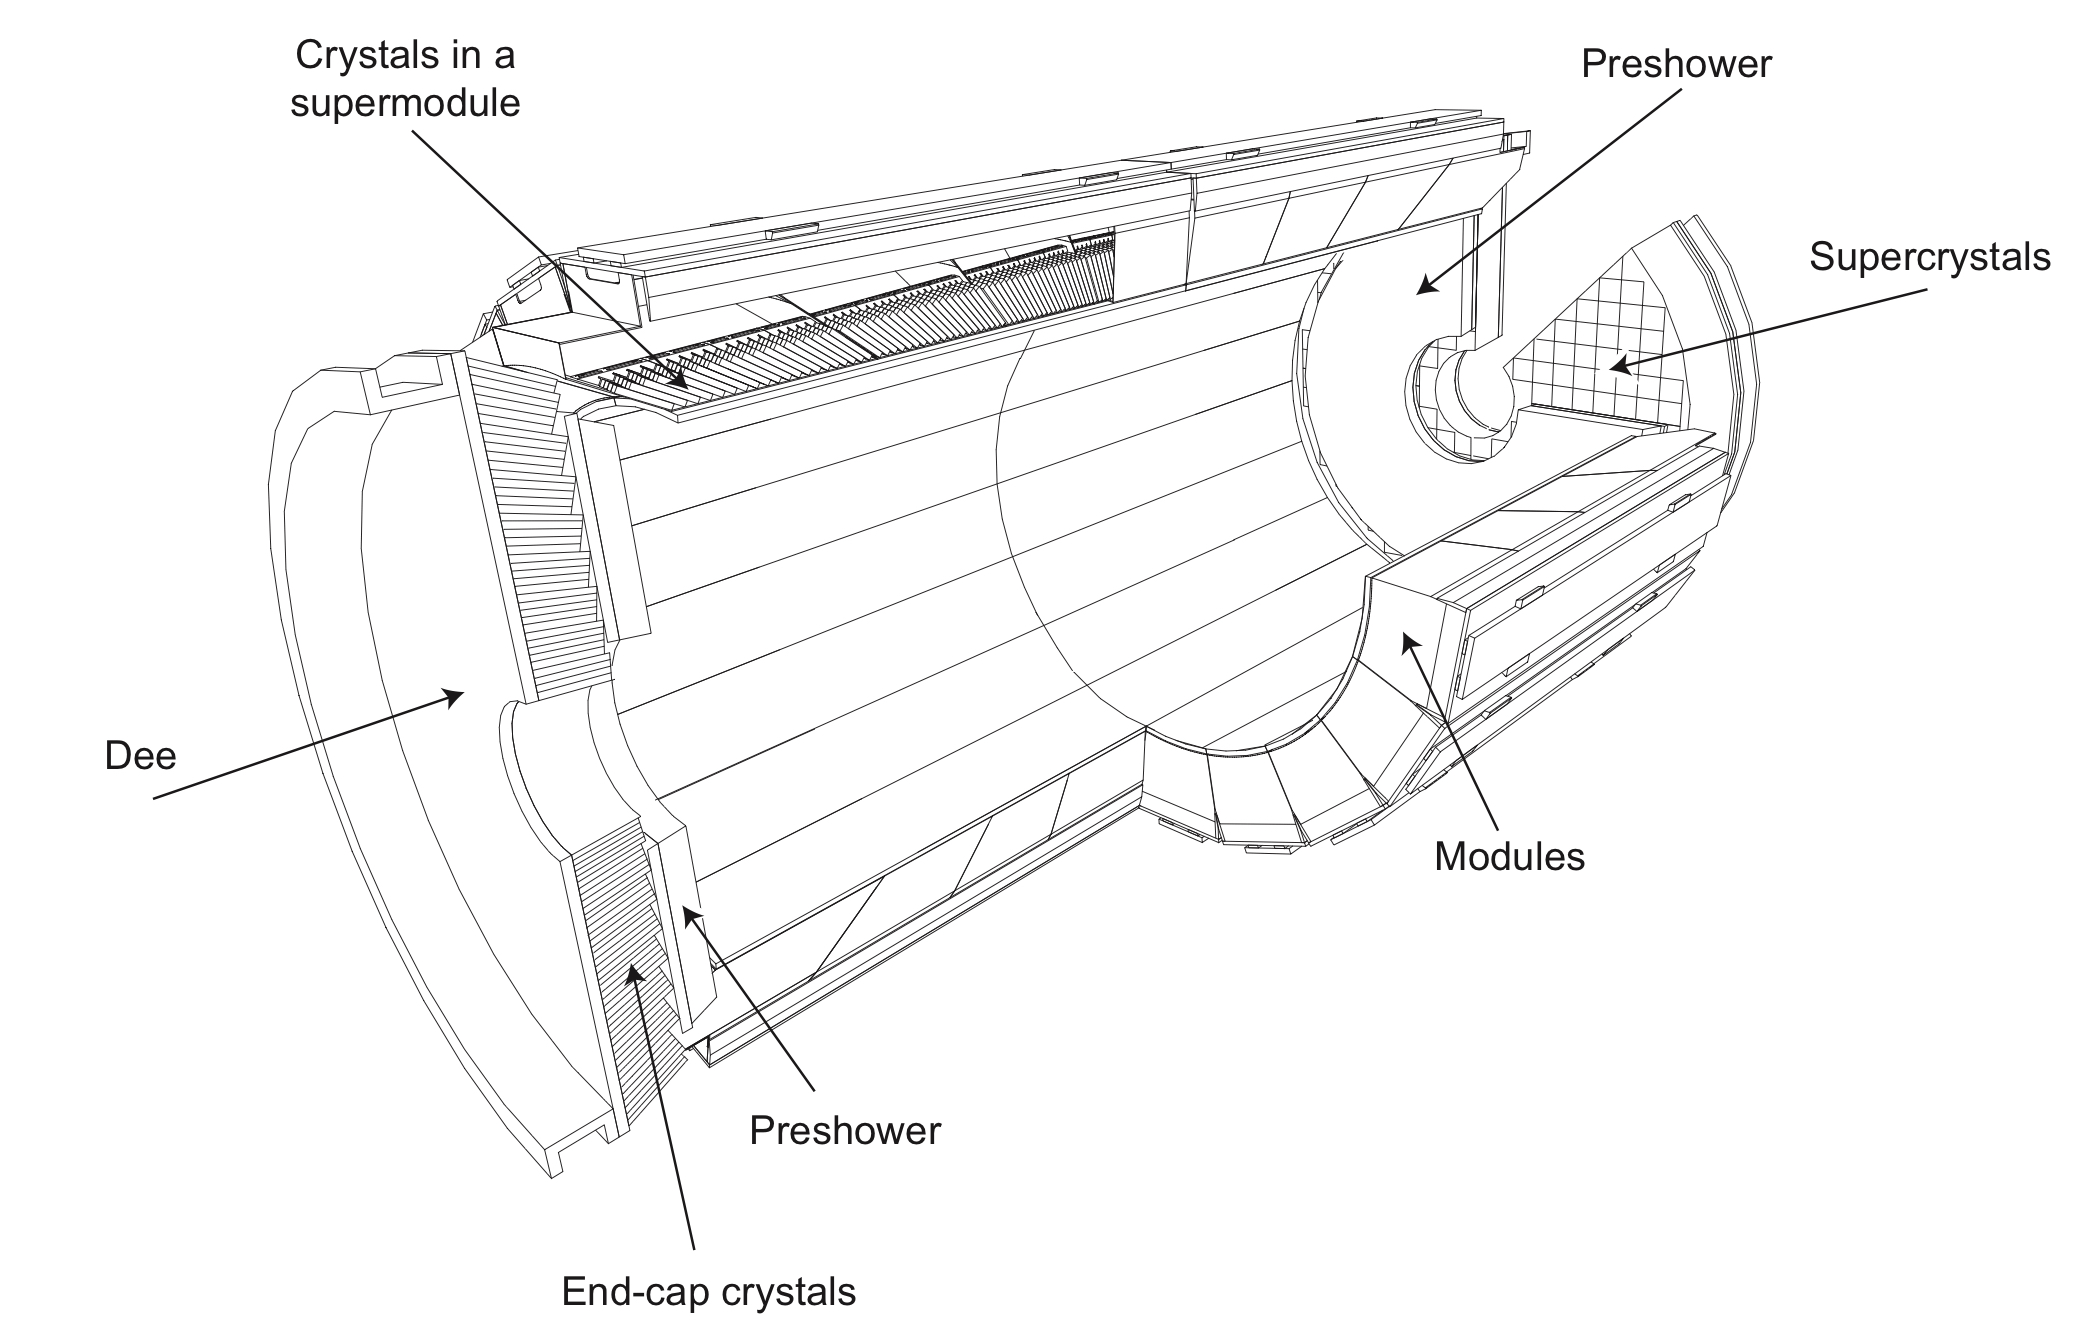
\includegraphics[width=0.49\textwidth,height=10cm,keepaspectratio]{figures/cms/ecal/xs_whiteblack.jpeg}
    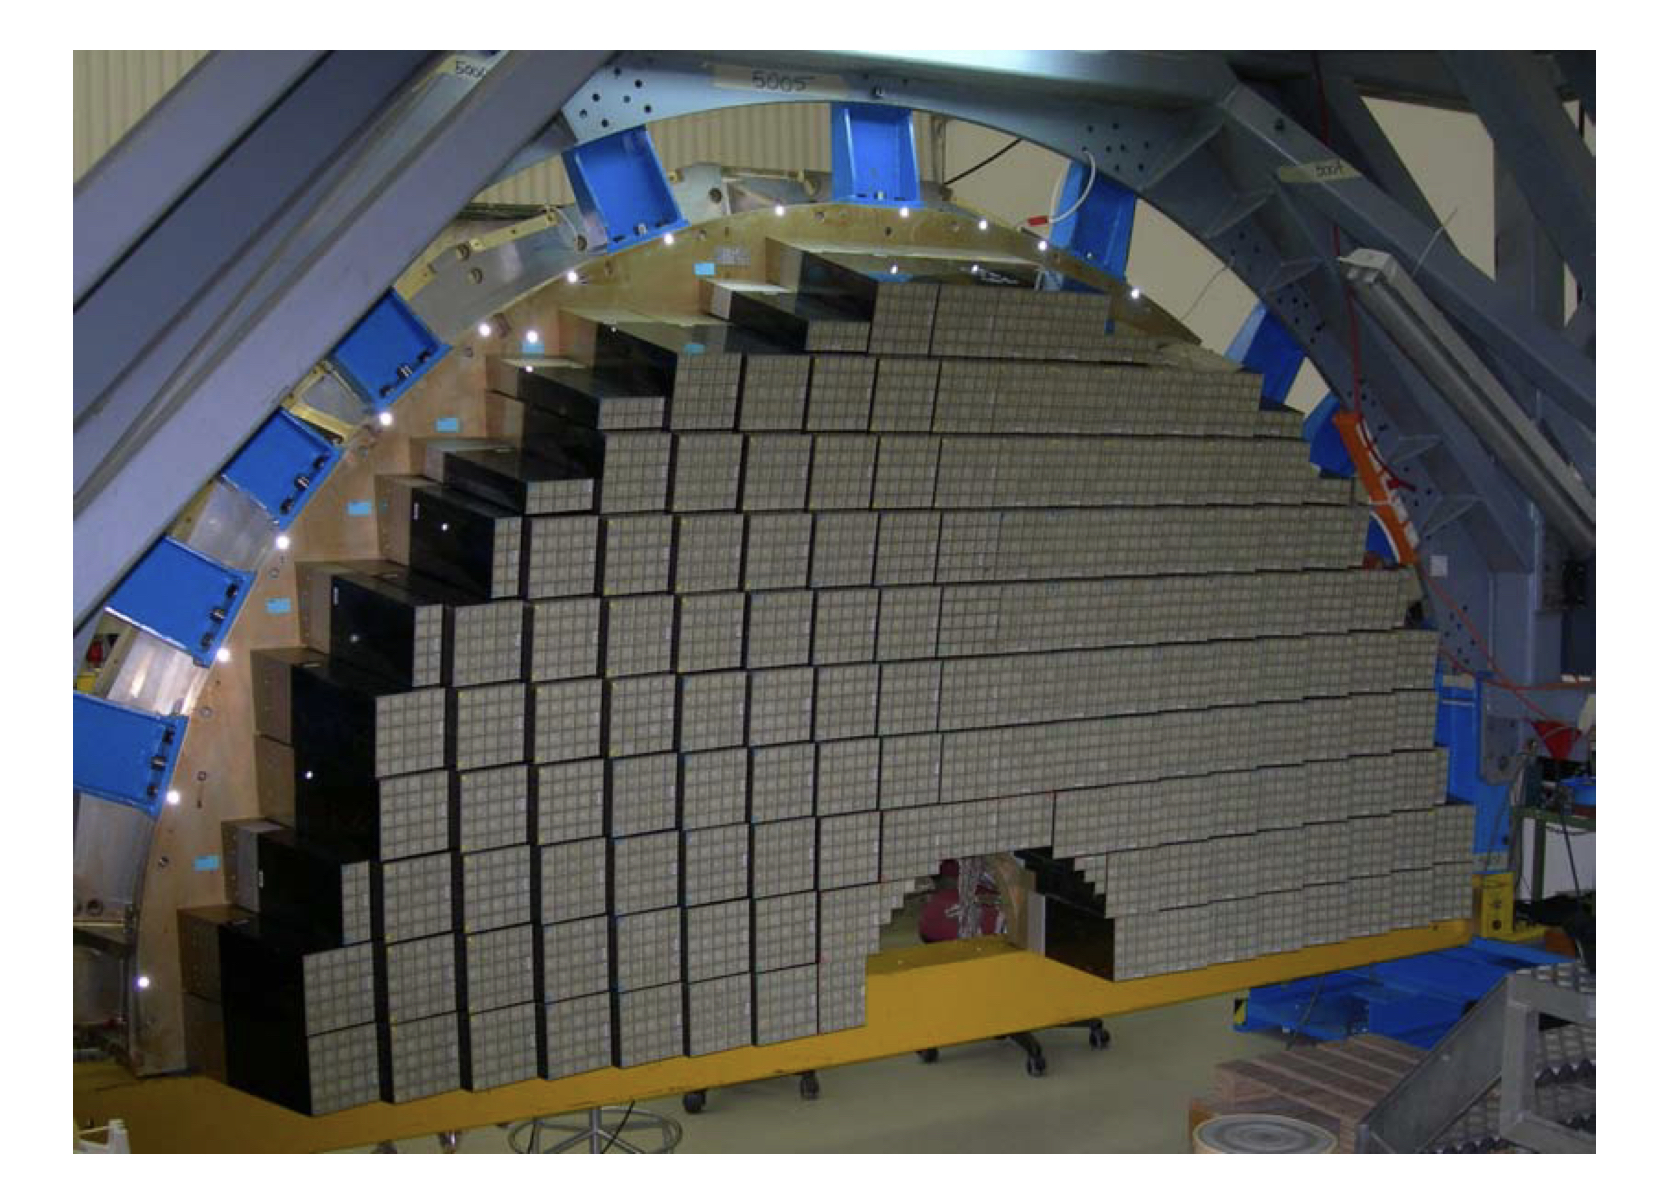
\includegraphics[width=0.49\textwidth,height=10cm,keepaspectratio]{figures/cms/ecal/dee.jpeg}
    \caption{
        (Left) Cross sectional view of the electromagnetic calorimeter of CMS.
        (Right) One of the Dees which comprise the EE.
        Each square of $ 5 \times 5$ crystals constitutes a ``supercrystal''.
        Figure taken from Ref.REFERENCE JINST%  ~\cite{jinst:cms_exp}.
        }
    \label{fig:ecal_xs}
\end{figure*}

%%%%%%%%%%%%%%%%%%%%
% ECAL Crystals
\begin{figure}[pbth]
    \centering
    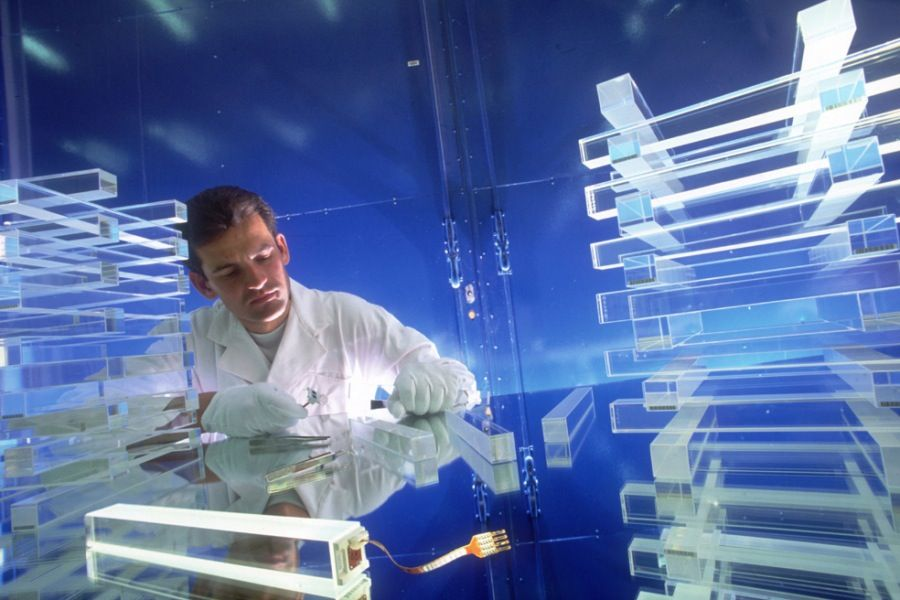
\includegraphics[width=0.49\textwidth,height=10cm,keepaspectratio]{figures/cms/ecal/ECAL_crystals_fancy_lab.jpg}
    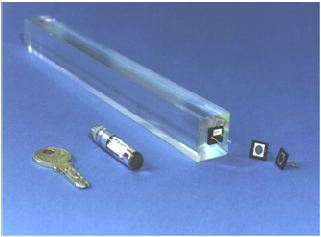
\includegraphics[width=0.49\textwidth,height=10cm,keepaspectratio]{figures/cms/ecal/ECAL_crystal_sizecomparison.jpg}
    \caption{
        (Left) ECAL crystals made from PbWO$_4$ are grown in a lab.
        (Right) Although made mostly of metal, ECAL crystals are transparent and have a photomultiplier detector attached at the end.} 
    \label{fig:ecal_crystals}
\end{figure}
%%%%%%%%%%%%%%%%%%%%

% PHYSICS
\textit{\textbf{Physics:}}
When electrons or photons pass through the ECAL, they create an EM shower.
Electrons radiate more photons as they accelerate around PbWO$_4$ nuclei, in a process called \emph{bremsstrahlung}.
Meanwhile, near the presence of a nucleus, high-energy photons pair produce into \ee.
% In turn, these newly-produced electrons can radiate more photons 
This cycle of electron and photon production disperses the initial particle energy into a spray of lower- and lower-energy particles; an EM shower (REFERENCE EM SHOWER FIG).

SHOW PICTURE OF EM SHOWER.

The ECAL crystals then scintillate (emits photons) in proportion to the amount of energy deposited by the interacting particle. 
The scintillator photons are detected by avalanche photodiodes on the back of each barrel crystal or by vacuum phototriodes in the endcap crystals (Fig.~\ref{fig:ecal_crystals}, Right).
Conveniently after 1 bunch crossing (25 ns), Approximately 80\% of the scintillated light is emitted.

An energy deposit in the ECAL could come from either an electron or a photon.
In order to tell the difference, information from the silicon tracker is used.
Charged particles, like electrons, will leave hits in the tracker and follow a curved path, whereas photons are electrically neutral and thus will not show any signs within the silicon tracker.
So long as the tracker and ECAL communicate effectively with each other, then they help distinguish between electrons and photons.
Charged hadrons interact only minimially with the ECAL, instead continuing on to the Hadron Calorimeter.
Neutral hadrons can be detected by the ECAL preshower near the ECAL endcaps which helps distinguish a single photon from $\pi^{0}$ mesons as they decay into two photons with a narrow opening angle, making it look as if the two photons are a single photon.
The preshower detector allows CMS to distinguish between low-energy diphoton pairs and single high-energy photons.

NEED SMOOTH TRANSITION INTO HCAL. What about those hadrons? They got through the ECAL... To detect hadrons effectively, we need a Hadron Calorimeter.
% That's what we see here with the blue dashed line (the photon) and the red line (the positron).

\subsection{Hadron Calorimeter}
\label{subsec:hcal}

% WHAT IT IS
\textit{\textbf{What is it?}}
The particles that survive the ECAL, typically only muons and hadrons, then enter the hadron calorimeter (HCAL).
Its primary purpose is to absorb the hadronic matter emerging from the interaction point and measure the corresponding jet energies.
The absorbed jets cause the HCAL to scintillate photons which are then converted into electrical signals.
These signals are used to deduce the original jet energies and any missing transverse energy (\MET) from the event.
% emit proportionally-energetic scintillated 

% STRUCTURE
\textit{\textbf{Structure:}}
Dissimilar to the ECAL (subsec.~\ref{subsec:ecal}) in material composition but similar in shape, the HCAL is a brass cylindrical scintillator.
Although it has a barrel (HB) and two endcaps (HE), it has two more detectors than the ECAL: the outer calorimeter (HO) and the forward calorimeter (HF).
The HB spans the pseudorapidity range $\abseta < 1.3$, the HE spans $1.3 < \abseta < 3$, and the HF spans $3 < \abseta < 5.2$, as shown in Figure~\ref{fig:hcal_quadrant}.
With a thickness of over $1\meter$, the HB is sandwiched between the barrels of the ECAL and the solenoid (subsec.~\ref{sec:solenoid}) at radial values $r = 1.77~\meter$ and $r = 2.95~\meter$, respectively.
Because the HB and HE are located within the solenoid's strong magnetic field of 3.8 \tesla, they both were both constructed out of a non-magnetic absorber called \emph{C26000 cartridge brass}.
This absorber has a density of 8.53 $\gram/\cm^{3}$ and an interaction length $(\lambda_I)$ of 16.42 \cm.
The thickness of the HB increases as $1/\sin{\theta}$ so that at $\abseta = 0(1.3)$ the absorber thickness is $5.82(10.6)~\lambda_I$.
The HB is composed of two half-barrels, where each half-barrel is built from 18 identical azimuthal wedges and each wedge spans 20$^\circ$.
Each wedge is divided into four $\phi$ segments so that a single $\phi$ segment spans $\Delta \phi = 0.087$.

Since the volume available to the HCAL is so limited, and in order to stop any particles that might traverse the entire HCAL and solenoid, the HO (the ``tail catcher'') is situated outside the barrel of the solenoid.
The HF is located 11.2 \meter from the interaction point.

All tiles within a single $\phi$ segment are grouped together into a single tray unit.
The scintillator is also segmented into 16 $\eta$ sectors, the first(last) of which is located at $\abseta = 0(1.3)$.
This way each tile covers $(\Delta \eta, \Delta \phi) = (0.087, 0.087)$.
Each layer has 108 trays.

%%%%%%%%%%%%%%%%%%%%
% HCAL Quadrant
\begin{figure}[pbth]
    \centering
    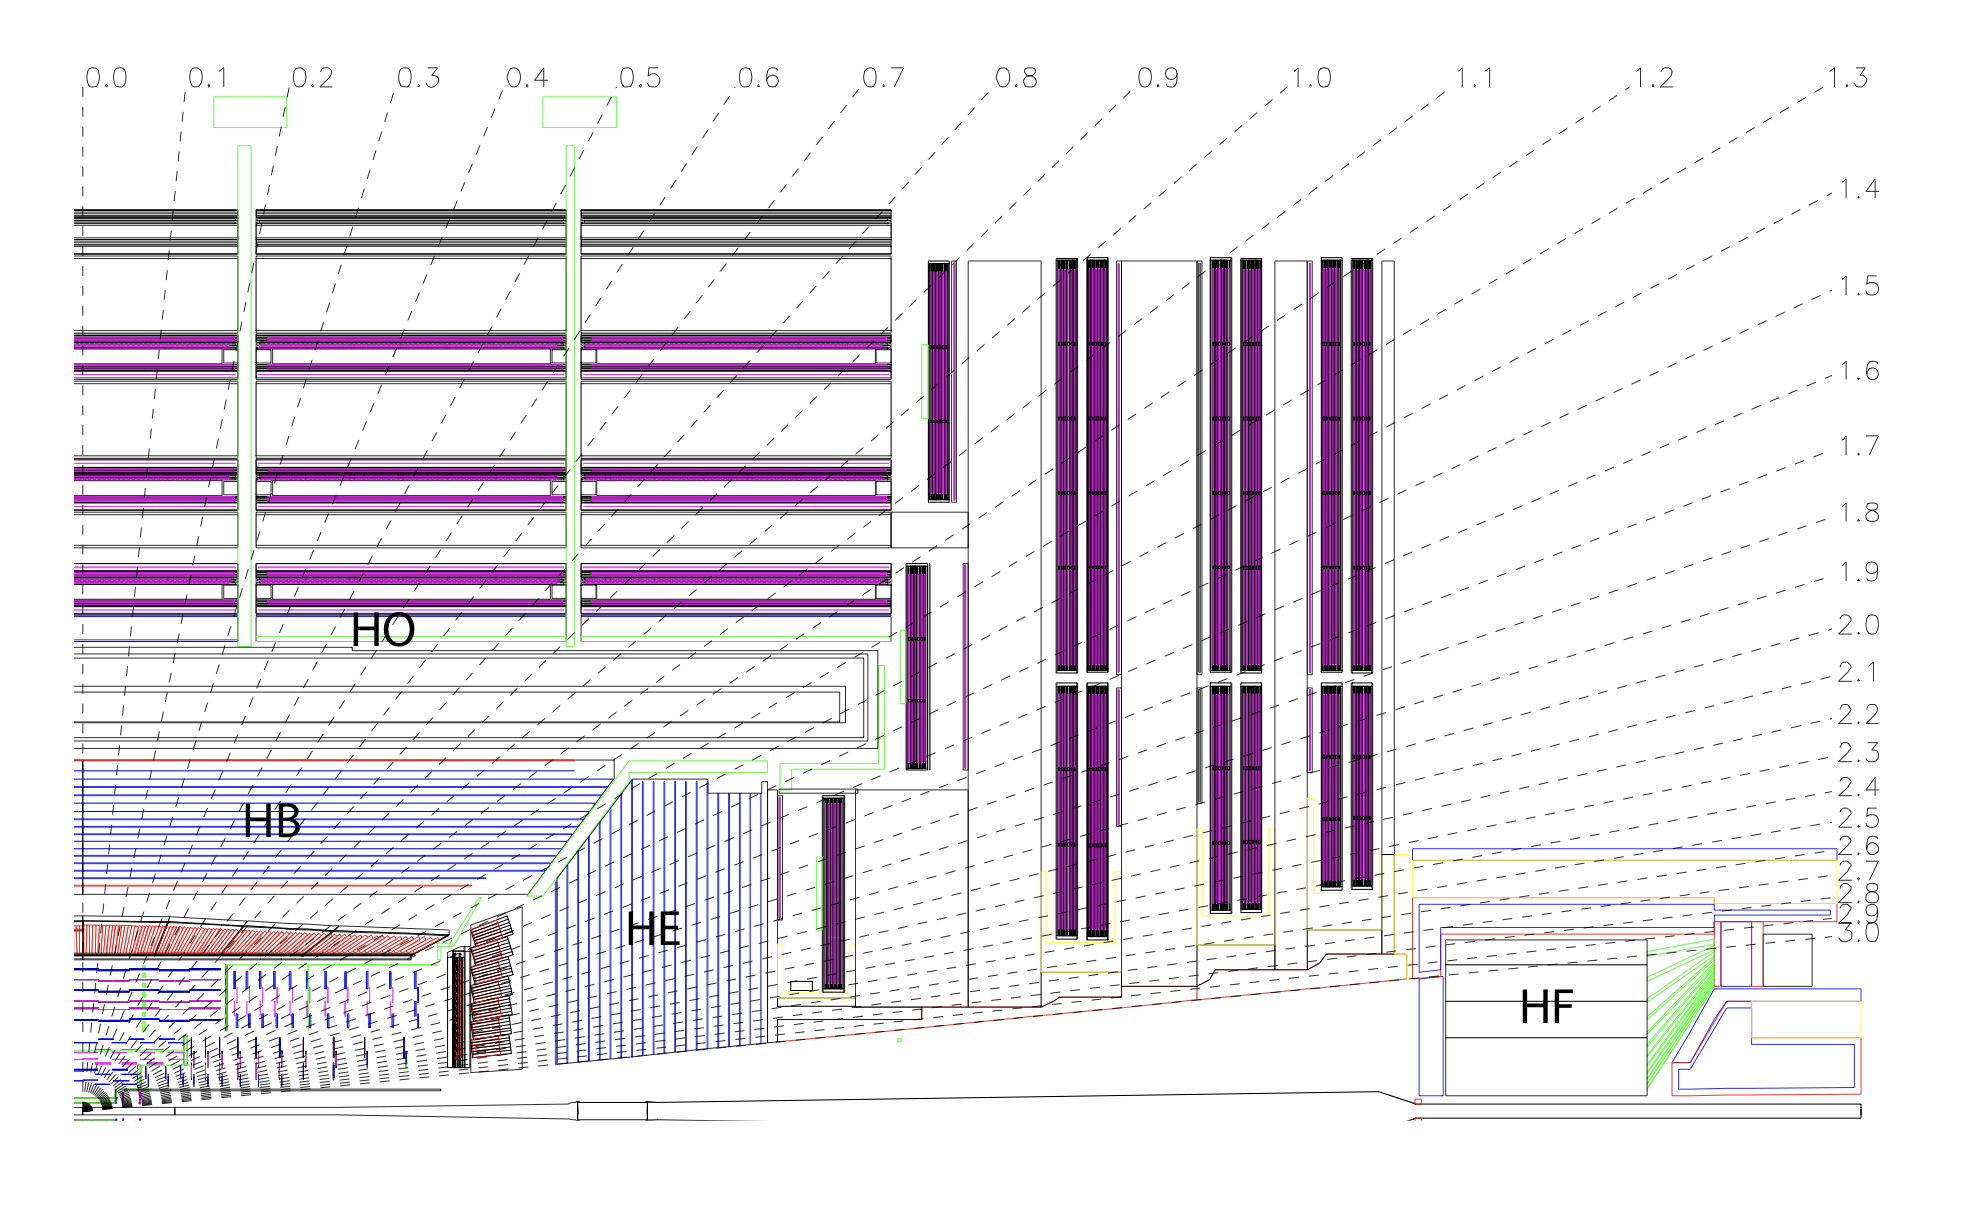
\includegraphics[width=0.95\textwidth]{figures/cms/hcal/hcal_quadrants_longitudinalview.jpg}
    \caption{
        A cross-sectional quadrant of CMS showing the locations of the HCAL components:
        the barrel (HB), outer (HO), endcap (HE), and forward (HF) detectors.
        }
    \label{fig:hcal_quadrant}
\end{figure}
%%%%%%%%%%%%%%%%%%%%

% PHYSICS
\textit{\textbf{Physics:}}
Since hadrons are the only particles to interact via the strong force, the HCAL is designed to have a high nuclear density.
This ensures ample opportunity for hadrons to radiate gluons and convert  with the Similar to the ECAL, the HCAL will scintillate in proportion to the amount of energy of the captured particle. 
The incoming hadrons will \emph{hadronize} (\ie, produce a hadronic shower), generating jets of quarks and gluons which are bound in various ways forming protons, neutrons, pions, kaons, \etc
Interestingly, the HCAL is made using over a million old, brass shell casings from the Russian Navy back from World War II.
% kinds of particles which have not decayed on their own or were not caught by the ECAL, ,  or when it catches hadronic material: stuff made of quarks, like . 

About 34\% of the particles produced from LHC \pp collisions enter the HE region, so the HE was built to handle high rates (MHz).

The entire HCAL utilizes approximately 70,000 plastic scintillator tiles.
The active material in the HB is 3.7-\mm-thick Kuraray SCSN81 plastic scintillator, selected for its radiation hardness and long-term stability.
Hadron showers -> tiles scintillate -> scintillated photons are collected by 0.94-\mm-diameter green double-cladded wavelength shifting (WLS) fibers (Kuraray Y-11), which carry the light to hybrid photodiodes (HPD).


% \section{The Solenoid and the Steel Return Yoke}
\label{sec:solenoid}

The Compact Muon \emph{Solenoid} sports one of the world's most energetic solenoids which is paramount to the success of CMS.
Particles that exit the HCAL (subsec.~\ref{sec:hcal}) arrive at the cylindrical magnet which is 12.5\meter in length, has a bore diameter of 6\meter (6.3\meter when cold), and generates a uniform 3.8\tesla magnetic field parallel to the beam line.
To produce such a large and uniform magnetic field inside the approximately 360$\meter^3$ volume (Fig.~\ref{fig:cms_magnetic_field}), an 18\,000 amp current travels through the 4-layer, superconducting, NbTi coils.
This magnetic field stores a massive 2.6\GJ of energy---approximately the kinetic energy of an Airbus A320 in flight---and is 100\,000 times stronger than Earth's magnetic field, as measured on the surface.
The magnet has such a large stored-energy-to-cold-mass ratio (11.6\KJ/Kg) that it experiences a physical deformation of 0.15\% while being energized.
%%%%%%%%%%%%%%%%%%%%
\begin{figure}[pbth]
    \centering
    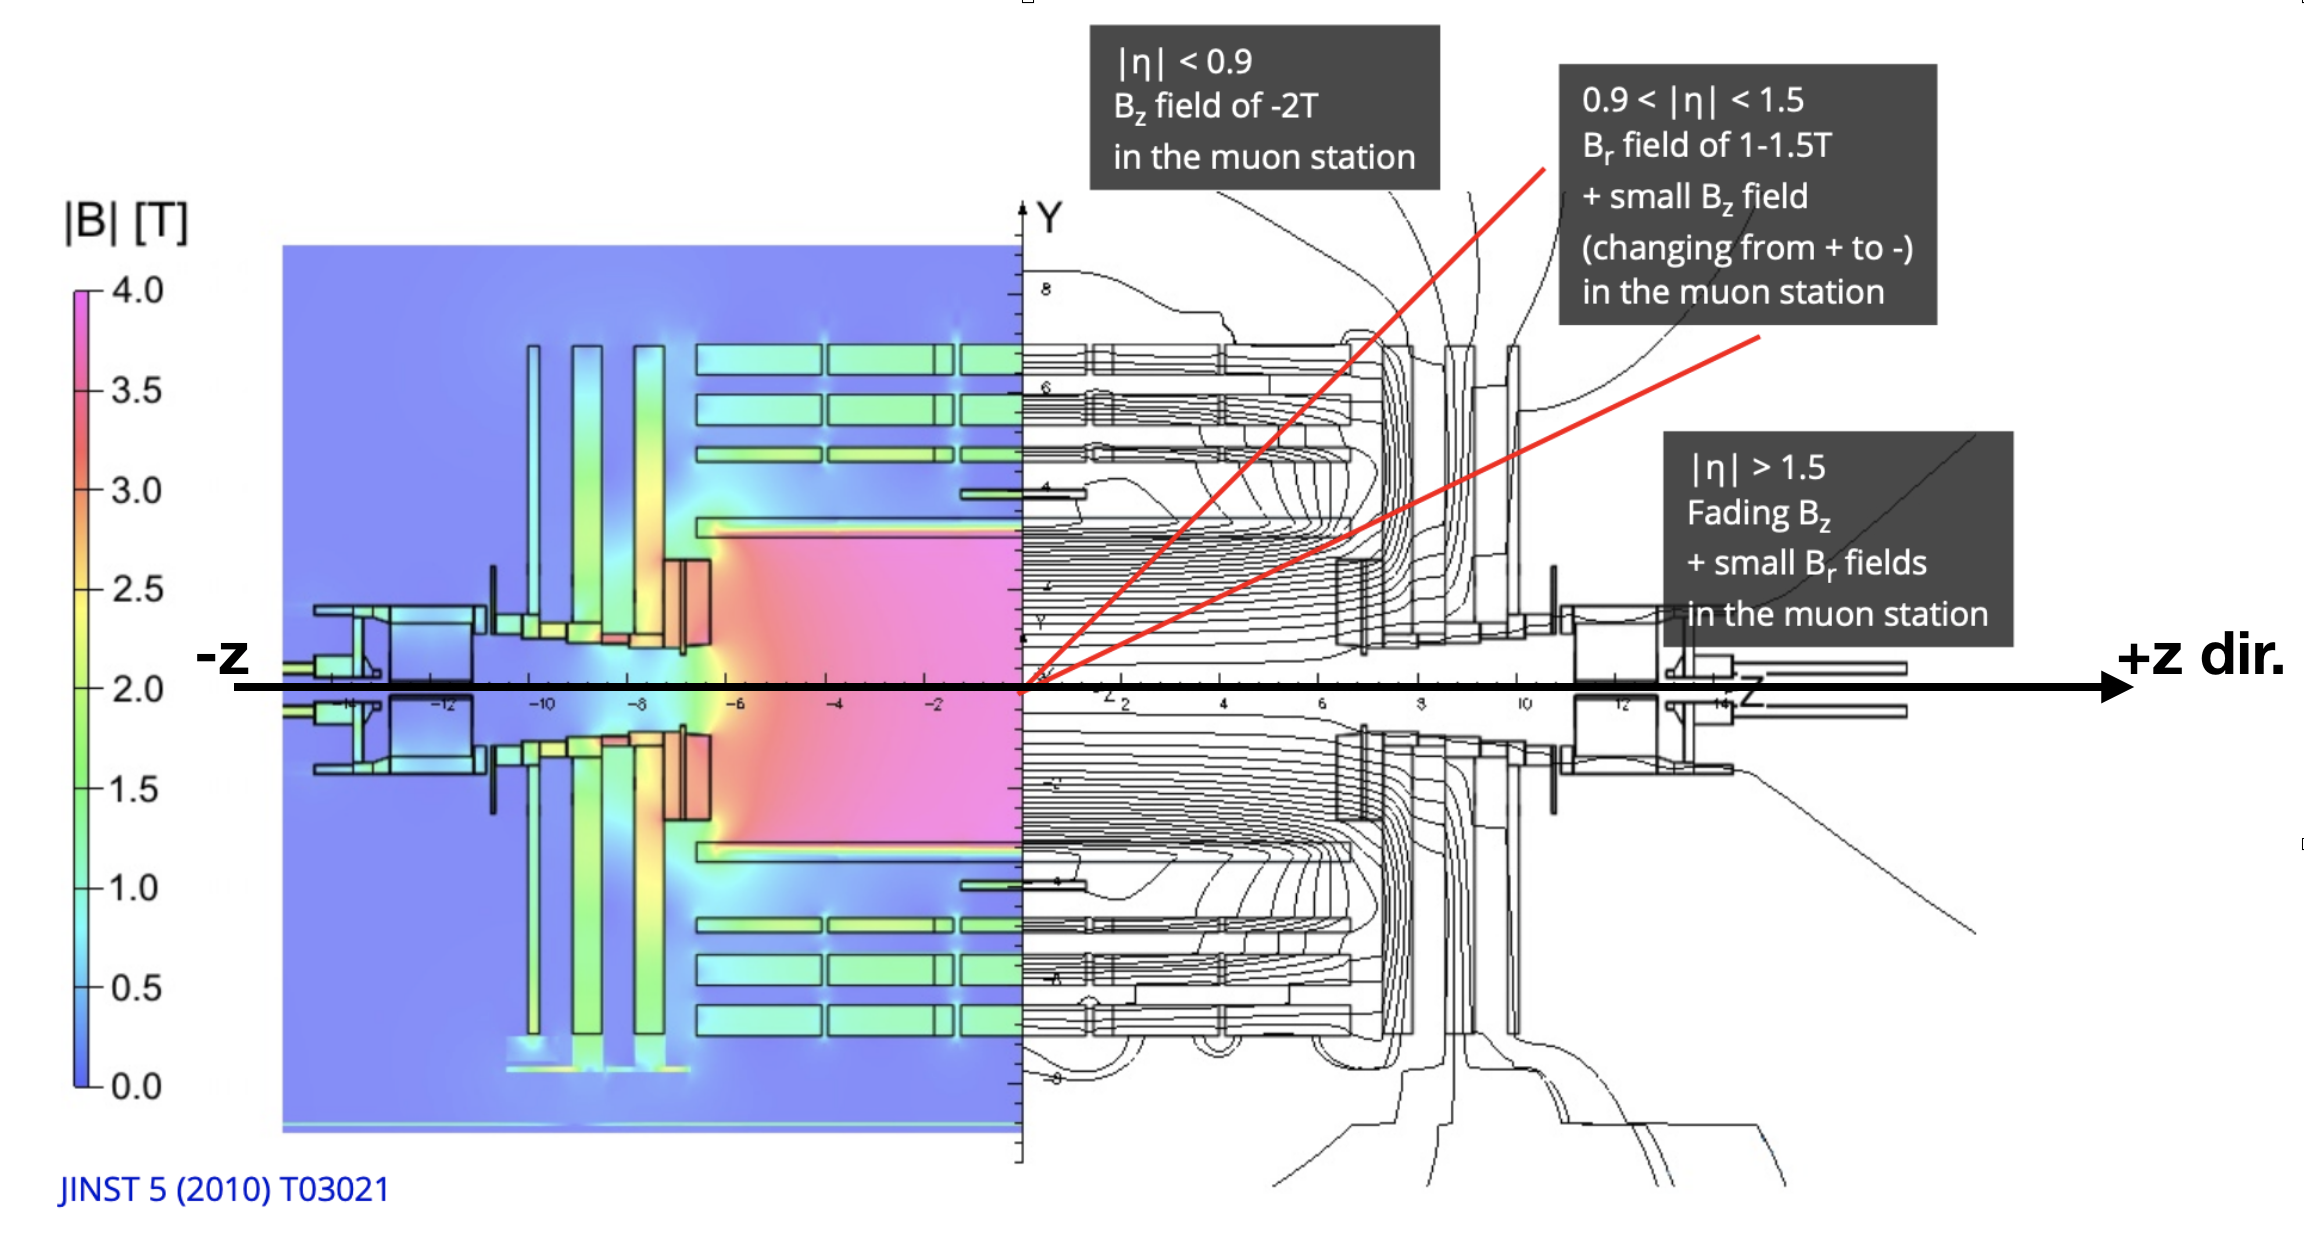
\includegraphics[width=15cm,height=15cm,keepaspectratio]{figures/cms/solenoid/CMS_longitudinal_view_magnetic_field.png}
        \caption{
        A longitudinal cross section of CMS showing the values of the magnetic field over the volume of CMS and various field lines. 
        The magnetic field reaches its maximum of 3.8 T in the center of the detector.}
        \label{fig:cms_magnetic_field}
    \end{figure}
    %%%%%%%%%%%%%%%%%%%%

As charged particles travel through any magnetic field, they experience a magnetic (Lorentz) force perpendicular to their direction of travel.
The Lorentz force $\left( \vec{F}_B \right)$ exerted on a particle with charge $q$ depends on the particle's velocity $\left( \vec{v} \right)$ and the magnetic field $\left( \vec{B} \right)$ via the cross product
\begin{equation*}
    \vec{F}_B = q \vec{v} \times \vec{B}.
\end{equation*}
Since the force is necessarily perpendicular to the velocity, the resulting trajectory is helical.
Projecting the helix on the $x$-$y$ plane (since the magnetic field points in the $+z$ direction) allows the particle tracks to typically be separated from one another.
Each track has a corresponding radius of curvature $\left( R \right)$ which relates to its transverse momentum $\left( \pt \right)$ through
\begin{equation*}
    \pt = qBR.
\end{equation*}
The relative change in \pt (\ie the \emph{momentum resolution}) is given by
\begin{equation}
    \frac{\delta \pt}{\pt} \propto \frac{\pt}{BL^2}.
\end{equation}

\textbf{Steel Return Yoke:} 
Most of the mass of CMS comes from the \emph{steel return yoke} which helps to redirect the magnetic field back on itself. 
The yoke system constitutes 10\,000 tonnes, which is 89\% of the total mass of CMS.
It is comprised of 5 wheels and 2 endcaps.

% \section{The Muon System}
\label{sec:muon_sys}

Although it is the farthest system from the interaction point, the muon system is one of the most important within the Compact \emph{Muon} Solenoid detector.
%  is the {\bf Muon System} and is what puts the {\it Muon} in Compact {\it Muon} Solenoid.
Of the particles emerging from the interaction point, electrons and photons are absorbed by the ECAL (subsec.~\ref{subsec:ecal}) and hadronic matter is absorbed by the HCAL (subsec.~\ref{subsec:hcal}).
This filtration process leaves only neutrinos and muons to enter the muon system, which is the outermost detector situated past the solenoid (sec.~\ref{sec:solenoid}).
As mentioned in
% section~\ref{sec:sm}
, neutrinos are the only weakly-interacting, electrically-neutral SM particles which makes them incredibly difficult to detect directly.
In fact, neutrinos interact with normal matter so little that a light-year (9.46 trillion\Km) of lead would only stop half of the neutrinos moving through it.
Thus, the detection of neutrinos produced from \pp collisions is inferred via \MET on a per-event basis.
Muons, on the other hand, have a mass of 105.7 \MeV (relatively heavy for a weakly-interacting, electrically-charged particle) and live a billion-billion times longer than a Higgs boson: the average lifetime of a muon is $\tau_{\mu} = 2.2 \times 10^{-6}$ s.
% which interestingly will travel way outside of CMS before decaying, upwards of 100s of kilometers before decaying to an electron and neutrino (neutrinos are the only particles which CMS can't explicitly detect).
These properties are what determined the properties of the muon system within CMS to consist of its four main subdetectors, each of which is described in the following subsections:
\begin{enumerate}
    \item CSC (cathode strip chambers, subsec.~\ref{subsec:csc}),
    \item DT (drift tubes, subsec.~\ref{subsec:dt}),
    \item RPC (resistive plate chambers, subsec.~\ref{subsec:rpc}),
    \item GEM (gas electron multiplier, subsec.~\ref{subsec:gem}).
\end{enumerate}

\subsection{Cathode Strip Chambers}
\label{subsec:csc}

\textit{\textbf{Overview:}}
A cathode strip chamber (CSC) is a multi-wire proportional chamber capable of precisely measuring the position of muons which enter and ionize the gas within.
Spatial coordinates are obtained by the collection of electrical signals along the cathode strips $(\phi)$, anode wires $(r)$, and across multiple CSC layers $(z)$.
CSCs are found exclusively on the two endcaps of CMS, with each endcap bearing 270 chambers (Fig~\ref{fig:cms_endcap}).
The chambers are arranged azimuthally around the beam pipe in four disks per endcap allowing for contiguous coverage in $\phi$.
In total, the CSC system provides an effective detection area of about 5,000$~\meter^2$, has a total gas volume that exceeds $>50~\meter^{3}$, and contains over 400,000 read-out channels.
%%%%%%%%%%%%%%%%%%%%
\begin{figure}[pbth]
    \centering
    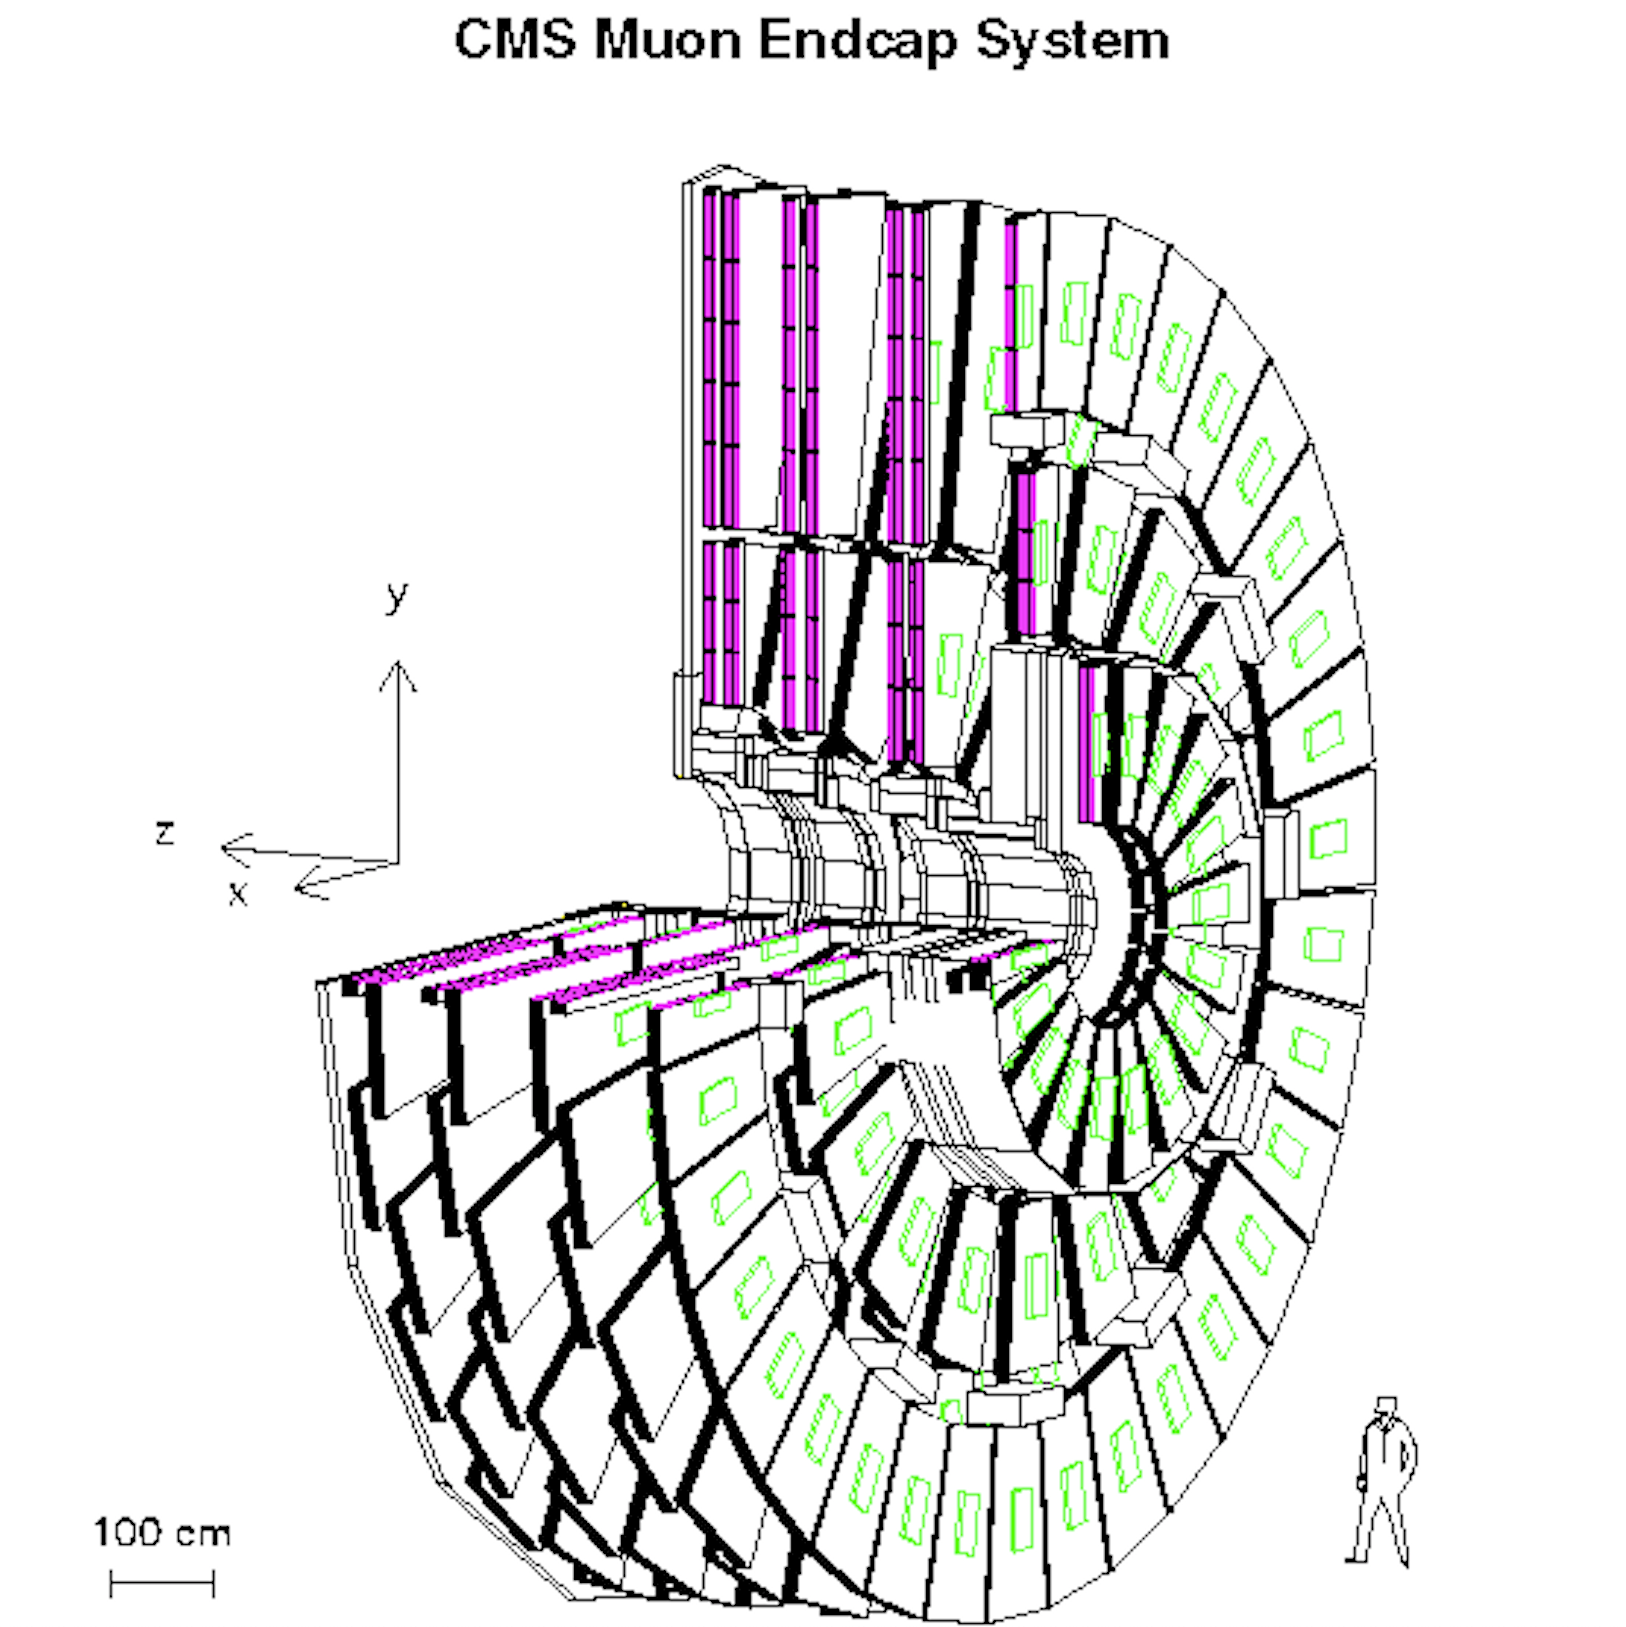
\includegraphics[width=0.49\textwidth,height=10cm,keepaspectratio]{figures/cms/muonsys/csc_endcap_cutaway.png}
    \includegraphics[width=0.49\textwidth,height=10cm,keepaspectratio]{figures/cms/muonsys/csc_endcap_real.png}
        \caption{
        (Left) A simulated cut out view of the ME+ endcap, with the coordinate system of CMS in the top-left corner.
        (Right) The actual ME-2 disk of CMS is shown, revealing its ME-2/1 and ME-2/2 rings of CSCs.
        }
    \label{fig:cms_endcap}
\end{figure}
%%%%%%%%%%%%%%%%%%%%

\textit{\textbf{Design:}}
Each CSC is trapezoidal in shape with its narrow end pointed toward the beam pipe (Fig.~\ref{fig:csc_guts}, Left).
The chambers are arranged in rings and each chamber subtends either 10$^\circ$ or 20$^\circ$ in $\phi$, as described in subsubsec.~\ref{subsubsec:csc_numbering}.
The CSCs cover the pseudorapidity range of $0.9 < \abseta < 2.4$ (Fig.~\ref{fig:cms_long_view_subdetectors}).
%%%%%%%%%%%%%%%%%%%%
% Longitudinal cross section
\begin{figure}[pbth]
    \centering
    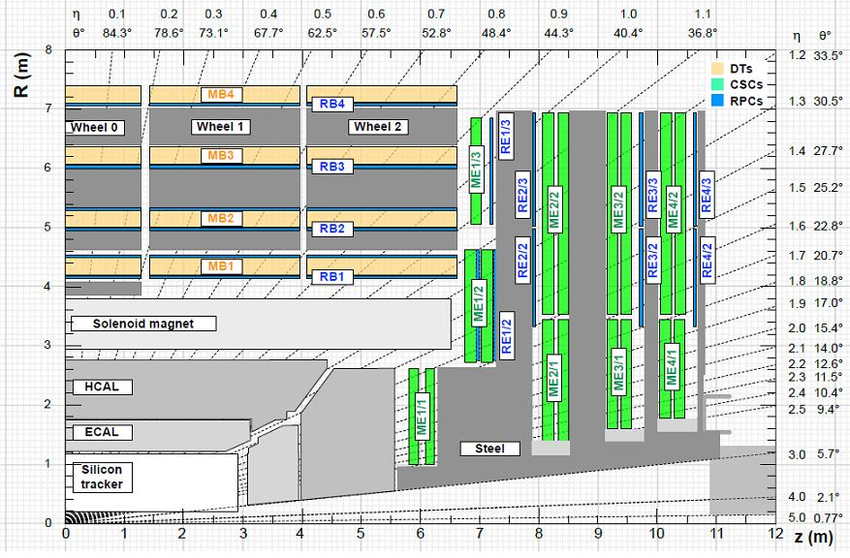
\includegraphics[width=15cm,height=10cm,keepaspectratio]{figures/cms/cms_longitudinal_view.png}
        \caption{
        Longitudinal cross section of CMS, showing the different pseudorapidity values ($\eta$) and also the different subdetector regions.
        }
        \label{fig:cms_long_view_subdetectors}
\end{figure}
%%%%%%%%%%%%%%%%%%%%
A single CSC is composed of six layers (or \emph{gas gaps}), each of which is filled with a carefully prepared gaseous mixture\footnote{
    The gas mixture ratio of Ar:CO$_{2}$:CF$_{4}$ was chosen to be 5:4:1 to maximize the lifetime of the CSCs as they endure radiation damage through years of use.
    The CO$_{2}$ is used as a non-flammable quencher to reach even larger electron multiplicities, while the CF$_{4}$ helps prevent polymerization along (aging of) the wires.
    }
of Ar:CO$_{2}$:CF$_{4}$ (Fig.~\ref{fig:csc_separatelayers}).
The gas mixture flows from one layer to the next in a zigzag manner and has a flow rate of ???.
Within every layer, the gas mixture surrounds approximately 80 copper strips, each of which spans radially away from the interaction point.
A single strip is about 8.4~\mm wide at the narrower end of the CSC, about 16~\mm at the wider end, and is separated from its neighboring strip by about 0.5~\mm.
Per layer, the inner gas also surrounds over 1,000 gold-plated tungsten wires, which are oriented azimuthally (so approximately orthogonal to the strips).
% (except in the CSCs closest to the interaction point)
Each wire is approximately 50~\mum in diameter and separated from its neighboring wire by about 3.2~\mm.
A collection of 16 consecutive wires forms a \emph{wire group}, which is about 5~\cm wide and creates a single anode read-out channel.
A single wire plane has five independently controlled HV segments (Fig.~\ref{fig:csc_guts}, Right).
The largest CSCs are 3.4~\meter long as measured along a strip and 1.5~\meter wide as measured along a wire.
% CSC separated layers.
%%%%%%%%%%%%%%%%%%%%
\begin{figure}[pbth]
    \centering
    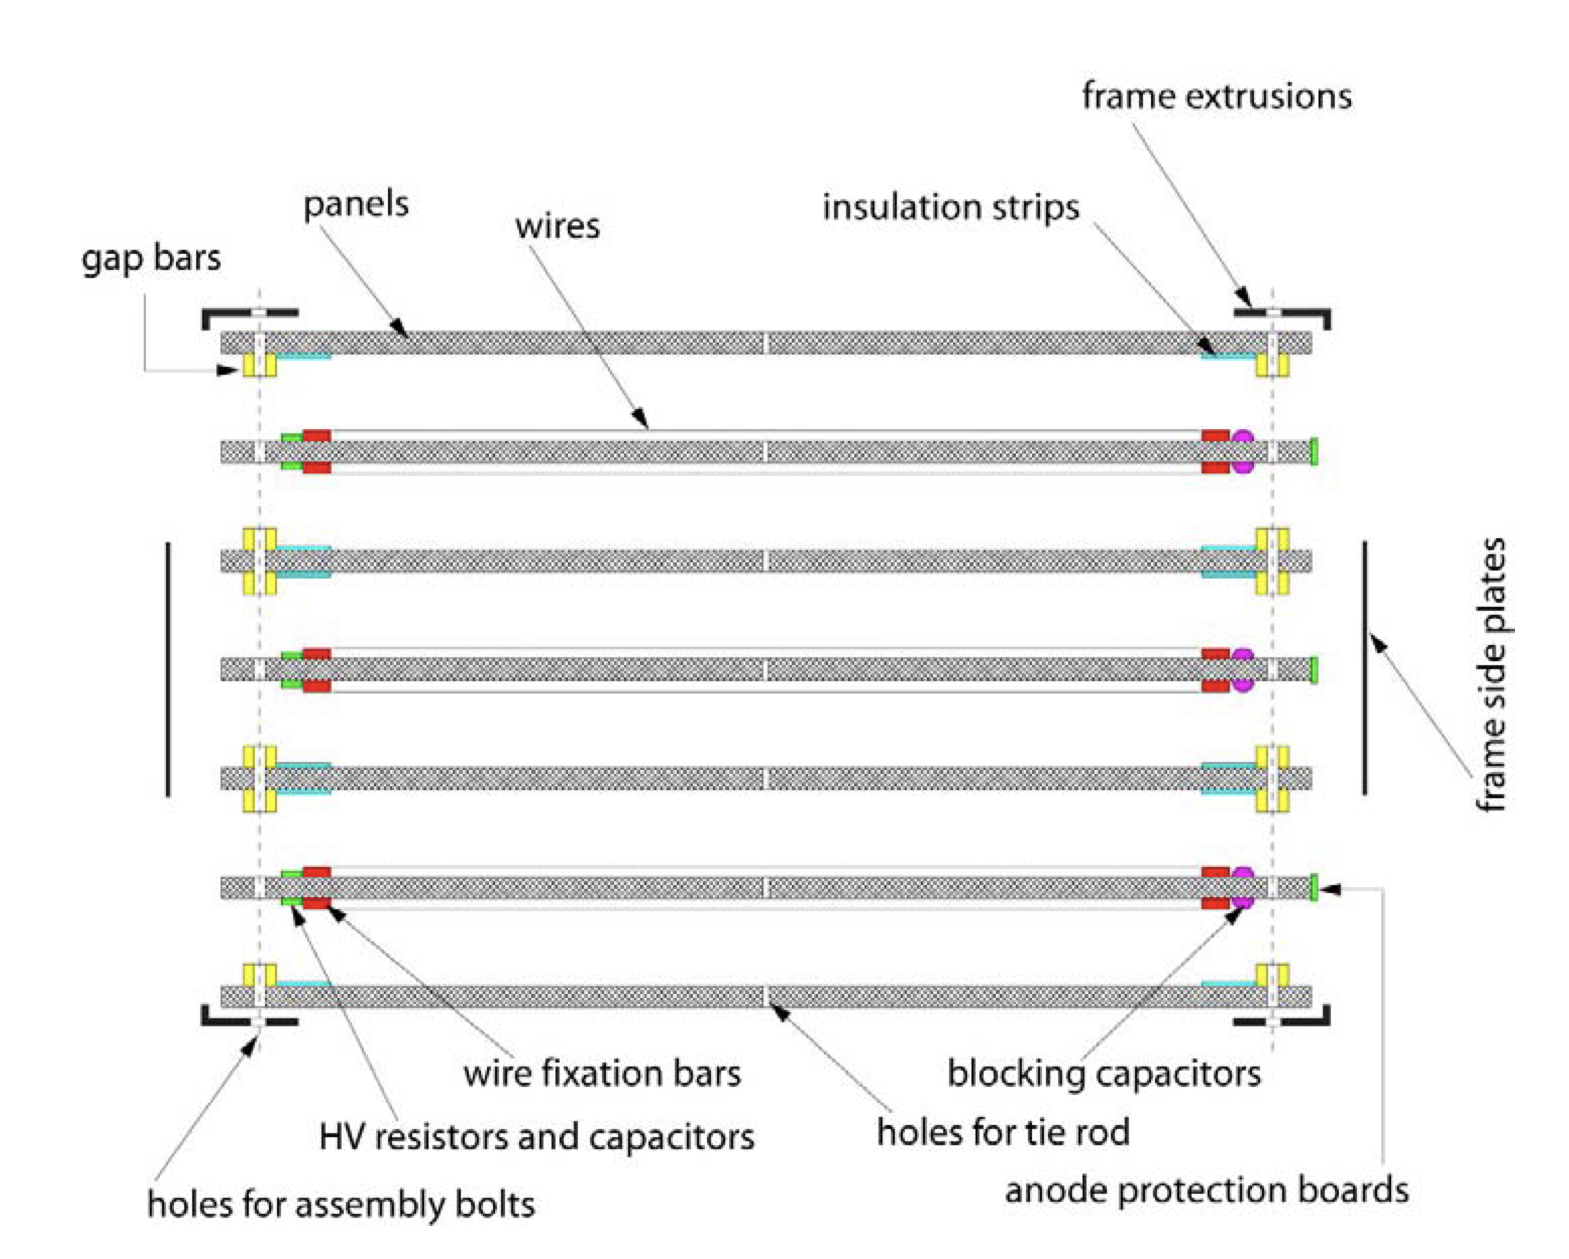
\includegraphics[width=15cm,height=10cm,keepaspectratio]{figures/cms/muonsys/csc_separatedlayers.jpeg}
        \caption{
        Exploded view of the cross section of a CSC showing how the 7 panels come together to form the 6 gas gaps between the panels.
        }
        \label{fig:csc_separatelayers}
\end{figure}
% CSC guts.
%%%%%%%%%%%%%%%%%%%%
\begin{figure}[pbth]
    \centering
    \includegraphics[width=0.49\textwidth,height=10cm,keepaspectratio]{figures/cms/muonsys/csc_cutaway_view_new.png}
    \includegraphics[width=0.49\textwidth,height=10cm,keepaspectratio]{figures/cms/muonsys/csc_stripsandwires.png}
        \caption{
        (Left) A CSC with its top layer exposed. You can see very thin gold-plated tungsten wires which actually span the entire width of the CSC. 
        Thicker vertical strips run along the length.
        (Right) More detail showing the radial strips and the horizontal wires. Also shown is the 5 segments of a CSC.
        }
        \label{fig:csc_guts}
\end{figure}
% In conjunction with the Silicon Tracker measurements, muon momentum can be measured to a precision of 
% {\bf Quick Mention:} The University of Florida has been one of the main contributors to the CSC system and was home to one of the testing and assembly facilities before shipping the CSCs off to CERN.

\textit{\textbf{Physics:}}
As a muon passes through a CSC layer, it has the opportunity to interact with and ionize an Ar atom in the gas mixture.
The wires are under high voltage (3,600 V) which causes the ionized electron to accelerate towards the positively-charged strips.
The accelerating electron collides with and ionizes Ar atoms along its path toward the strip.
This liberates even more electrons, thus forming an \emph{electron avalanche} (Fig.~\ref{fig:elec_avalanche}).
The total number of ionized electrons per initial electron is referred to as the \emph{multiplicity} (or \emph{gas gain}), which can reach as high as 100,000.
% Electron avalanche.
%%%%%%%%%%%%%%%%%%%%
\begin{figure}[pbth]
\centering
\includegraphics[width=15cm,height=10cm,keepaspectratio]{figures/cms/muonsys/csc_elec_avalanche_old.png}
    \caption{
    A muon passes through one of the gaseous layers of the CSC, ionizing the gas mixture and inducing a charge on the anode wires and cathode strips. 
    }
    \label{fig:elec_avalanche}
\end{figure}
%%%%%%%%%%%%%%%%%%%%

The electron avalanche is collected by a cathode strip and becomes an electrical signal.
This signal is processed by the cathode front-end boards (CFEBs).
The Ar$^+$ ions similarly distribute a charge signal onto the negative wires.
The cluster of charge that arrives at a strip is more widely spread than the charge which arrives along a wire.
Therefore, comparator logic is implemented on the strips to narrow down the precision to the order of 100~$\mum$ by using half-strip information (Fig.~\ref{fig:comparators}).
% Comparators and strips.
%%%%%%%%%%%%%%%%%%%%
\begin{figure}[pbth]
\centering
\includegraphics[width=15cm,height=10cm,keepaspectratio]{figures/cms/muonsys/csc_comparators_and_strips.png}
    \caption{
    (Left) Comparators are used to compare neighboring strip cluster charge to determine on which half-strip the peak charge resided.
    (Right) A muon passes through all six layers of a CSC inducing charge on various half-strips.
    % cathode front-end board (CFEB) 
    }
    \label{fig:comparators}
\end{figure}
%%%%%%%%%%%%%%%%%%%%

The muon passes through the next 5 layers of the CSC, further ionizing the gas mixture and generating electrical signals along the wires and strips.
A signal on a wire provides an $r$-coordinate, on a strip provides a $\phi$-coordinate, and through the other layers provides a $z$-coordinate.
Taken together, this information helps to reconstruct the three-dimensional trajectory of the muon.
% The AFEBs then digitize this analog signal using ADCs and 

The number of hits recorded by the CSC will determine if an event was significant enough to be worth saving.
If so, then its precise positions on the wires and strips will be read out by the Data Acquisition (DAQ) system and be stored for further data analysis.
When a CSC is taking live data it can resolve approximately 2~$\mm$ in $r$-$\phi$, whereas during offline analysis the resolution improves by a factor of more than 20:
the ME1/1 and ME1/2 chambers can resolve distances as small as 75~$\mum$ in $r$-$\phi$, while the other chambers can resolve 150~$\mum$.
It is worth noting that a CSC can accommodate up to 1 KHz/$\cm^2$.

% Each CSC cost about \$100,000 to make, so very quickly this becomes an expensive project.

Gas gap is 9.5~\mm.

% \subsection{Endcap Muon Electronics}
% In order to conclude that a muon definitely passed by the muon detectors, a very sophisticated electronics system has been developed. 

% Hmm... EMU is just for the endcaps. This system is called "EMU" and 

% Next I am going to elaborate more on the CSCs, since my first experience with CMS hands-on work with CSCs. 

% The muon barrel system, after it talks with the tracker system, has a muon pT resolution of 1.5% in the barrel and ~6% in the endcap.

% Trigger system:
% Since the event  rate and data rate are so high, and most of the events are uninteresting, typical physics,
% we need a fast-working filtration system to sift through the good and bad events. 
% We want to "trigger" on the good events but only have about 4 μs to do so. 
% This is the job of the L1 trigger and and the High-Level Trigger. 

\subsubsection{CSC Numbering Scheme}
\label{subsubsec:csc_numbering}
The two endcaps are labelled as ``ME+'' and ``ME-'', depending on whether they are situated in the +$z$ direction or -$z$.
Both endcaps are structurally symmetric, so it is sufficient to discuss only one in detail.
The ME+ endcap has four disks: ME+1 is the first disk and the one closest to the interaction point, while ME+4 is the fourth and the farthest away. 
Within each disk, there are either two or three ``rings'' of CSCs, as shown in Fig.~\ref{fig:cms_long_view_subdetectors} (green).
These rings are labelled as ME+$D$/$R$, where $D$ indicates the disk number and $R$ indicates the ring number.
For example, ME+2/1 refers to the second disk and the first ring (the ring closest to the beam pipe).
All rings contain 36 CSCs, except for ME$\pm X$/1, for $X= 2,3,4$, which contain only 18 CSCs.
Finally, the CSCs are given one final number to label them on the ring:
the CSC that sits along the positive $x$-axis in the coordinate system of CMS is given the number ``01'', \eg ME+4/2/01. 
The CSCs are then numbered incrementally following the positive azimuthal direction.

\subsection{Drift-Tube Chambers}
\label{subsec:dt}

\textbf{\textit{Overview:}}
Functionally similar to but structurally different from a CSC (subsec.~\ref{subsec:csc}), a DT is a collection of gaseous detector cells (Fig.~\ref{fig:dt_superlayers}).
A single DT cell has an anode wire and two cathode strips and operates on the same principle as a CSC, providing timing and position measurements of muons (Fig.~\ref{fig:dt_cell}).
While CSCs are found only on the endcaps of CMS, drift-tube chambers (DTs) are placed exclusively along the barrel (Fig.~\ref{fig:dt_locations}).
The DT system is therefore composed of concentric cylindrical stations, with the central axis parallel to the beam pipe.
Altogether, there are 250 DTs built inside of, between, and outside of the iron yoke.
% DT Chamber.
%%%%%%%%%%%%%%%%%%%%
\begin{figure}[pbth]
    \centering
    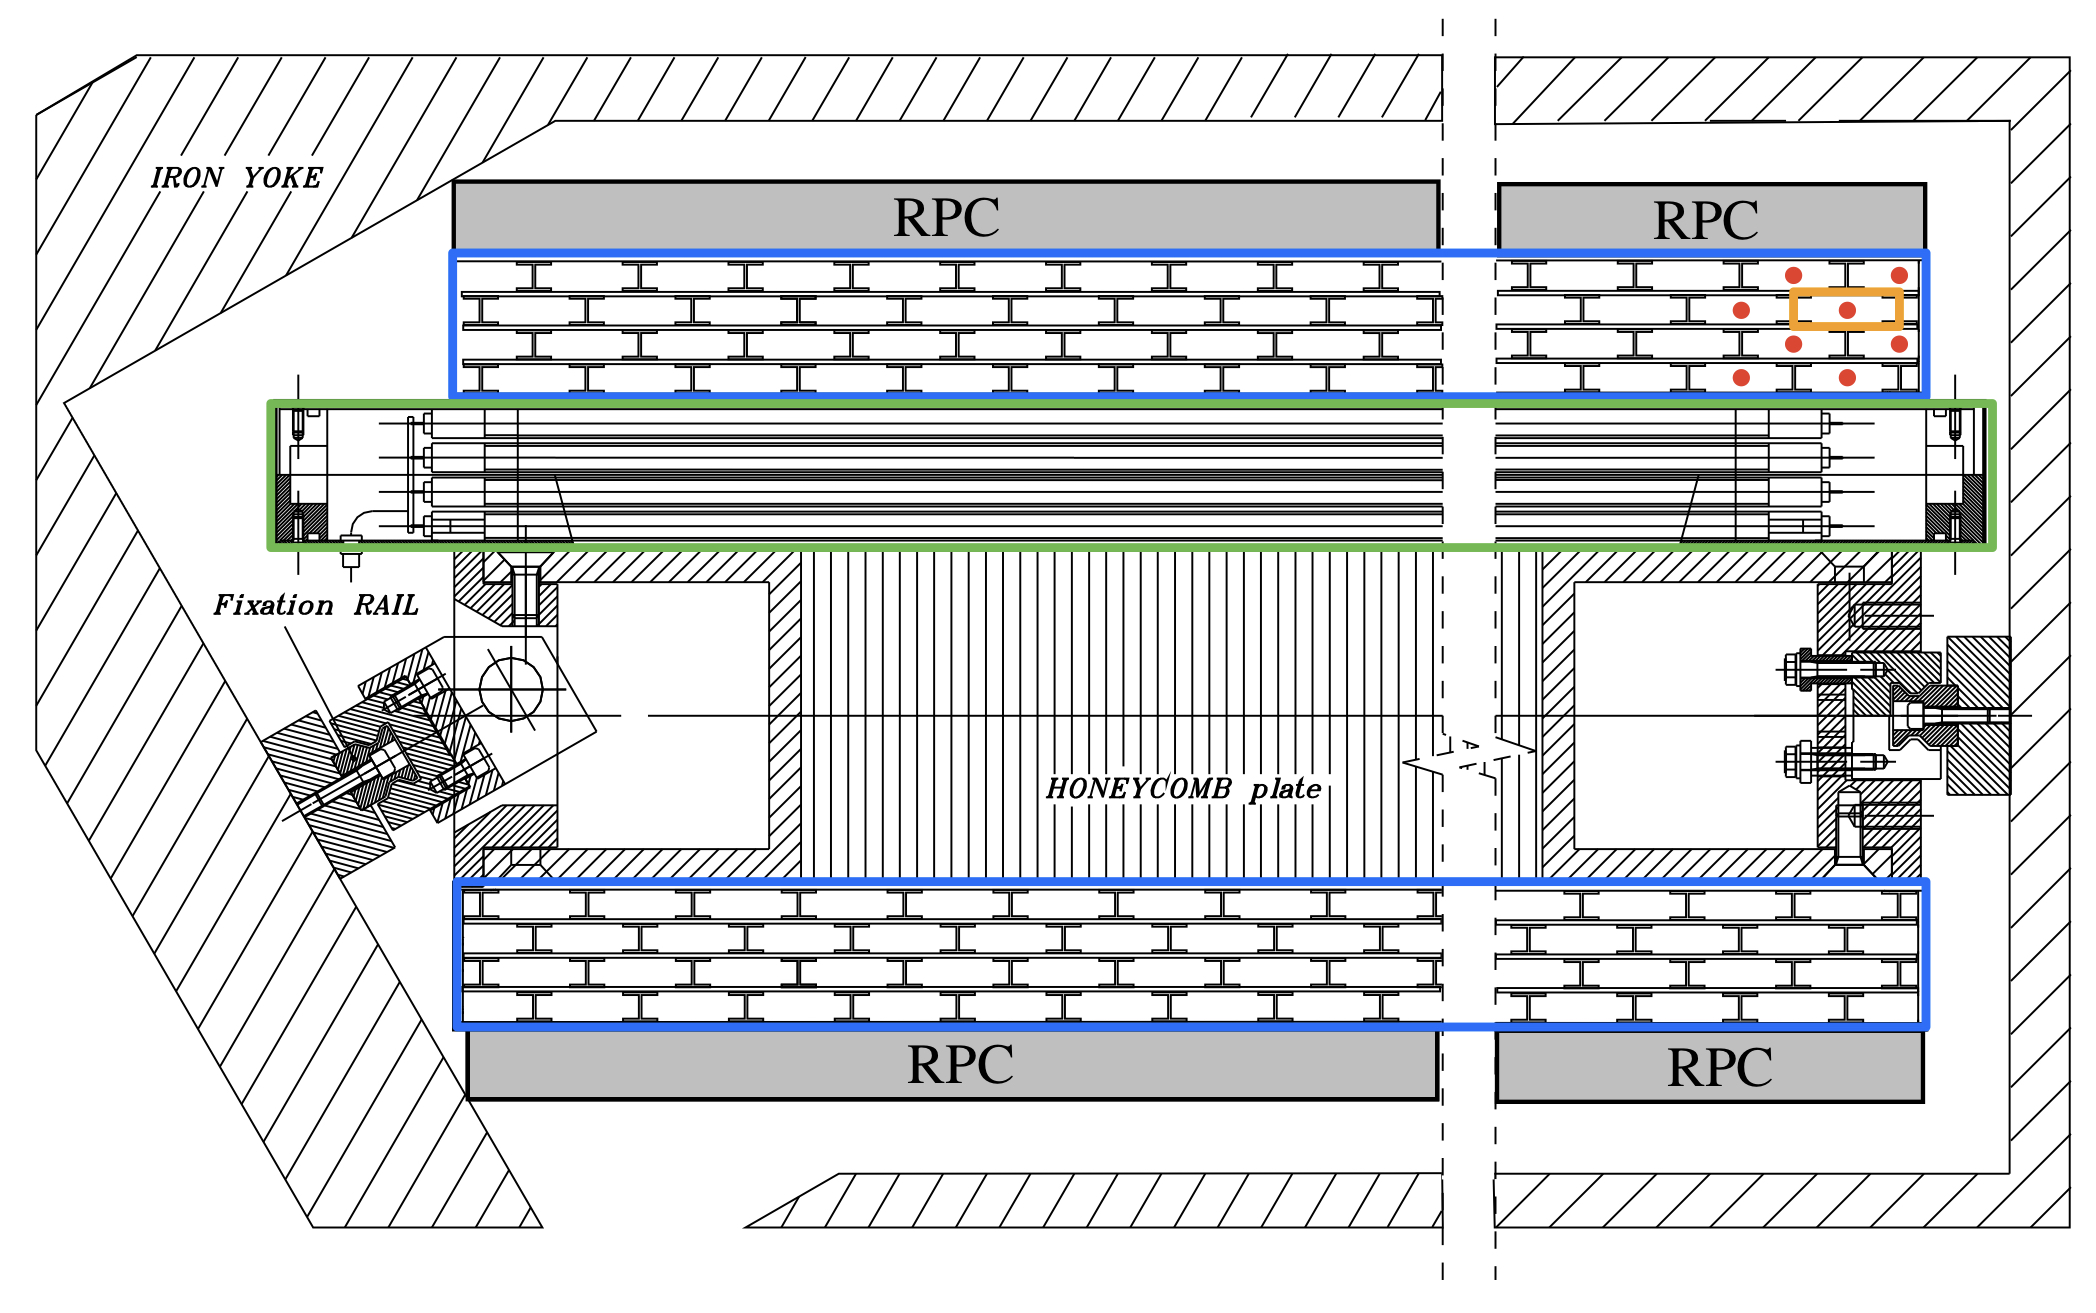
\includegraphics[width=15cm,height=10cm,keepaspectratio]{figures/cms/muonsys/drifttube_superlayers.jpeg}
        \caption{
        A drift-tube chamber with 3 superlayers (SLs) is sandwiching a honeycomb plate.
        Two SLs are indicated by the blue rectangles, whose cells (orange rectangle) have anode wires (red dots) oriented parallel to the beam pipe.
        The third SL is indicated by the green rectangle and is staggered orthogonally to the other two SLs.
        }
        \label{fig:dt_superlayers}
\end{figure}
% DT Cell.
%%%%%%%%%%%%%%%%%%%%
\begin{figure}[pbth]
    \centering
    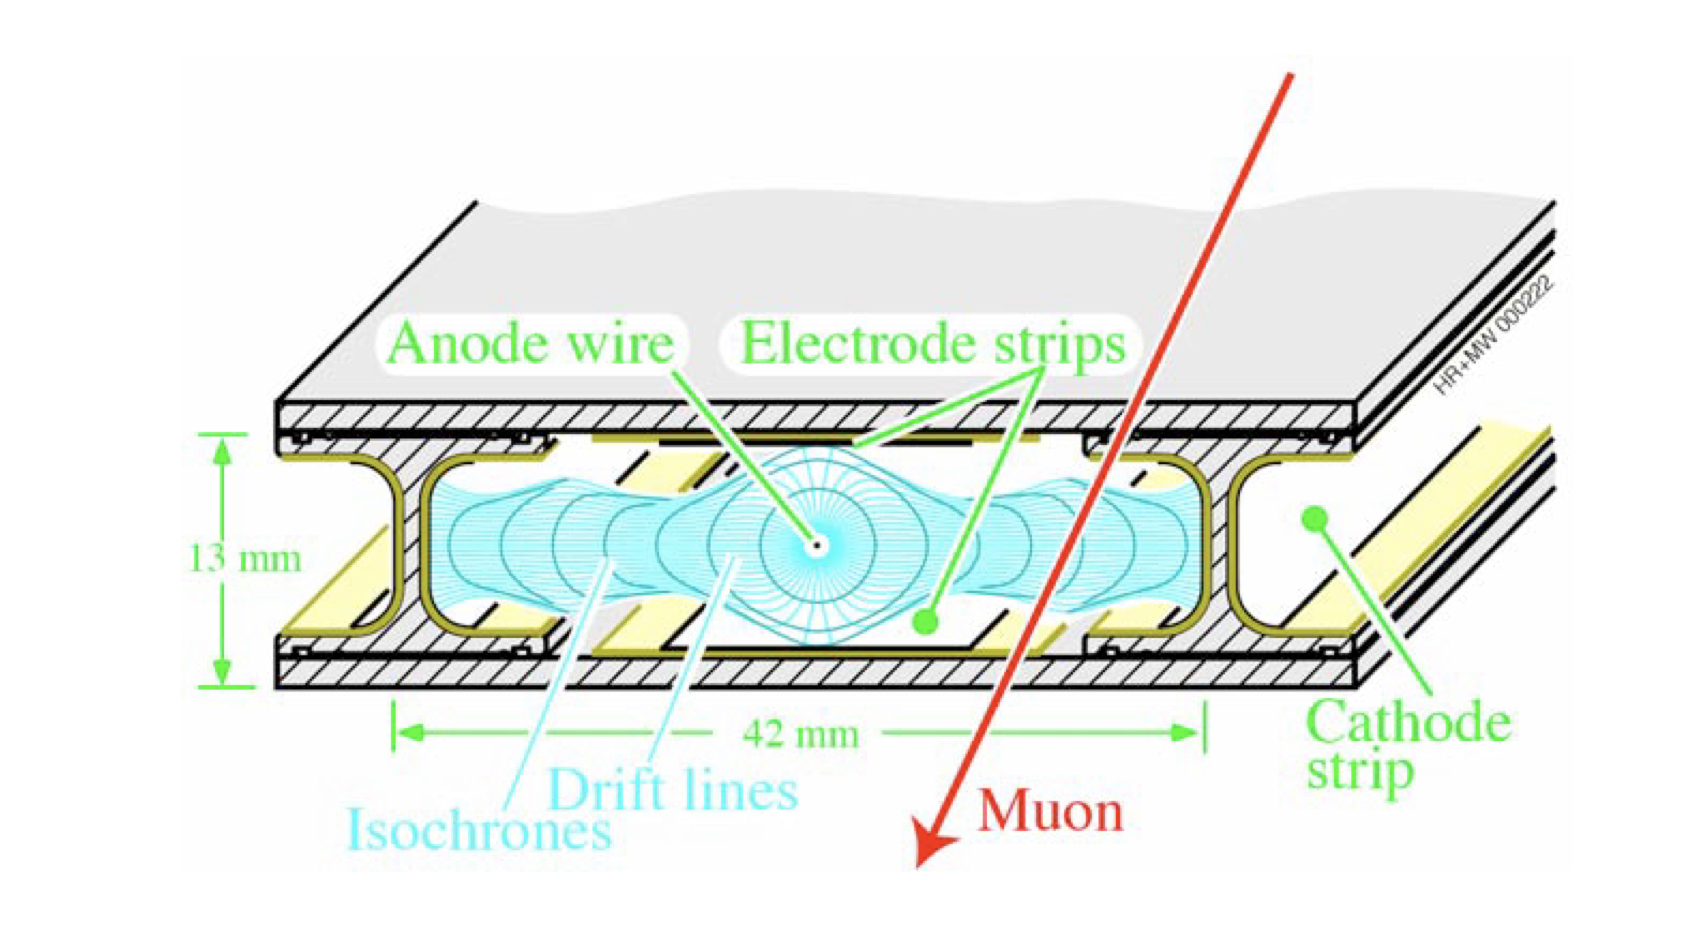
\includegraphics[width=15cm,height=10cm,keepaspectratio]{figures/cms/muonsys/drifttube_xs.jpeg}
        \caption{
        A cross section of a DT cell showing the drift lines (light blue), isochrone lines (dark blue), dimensions of the cell, and locations of the anode wire and cathode strips.
        }
        \label{fig:dt_cell}
\end{figure}
%%%%%%%%%%%%%%%%%%%%
% DT locations.
\begin{figure}[pbth]
    \centering
    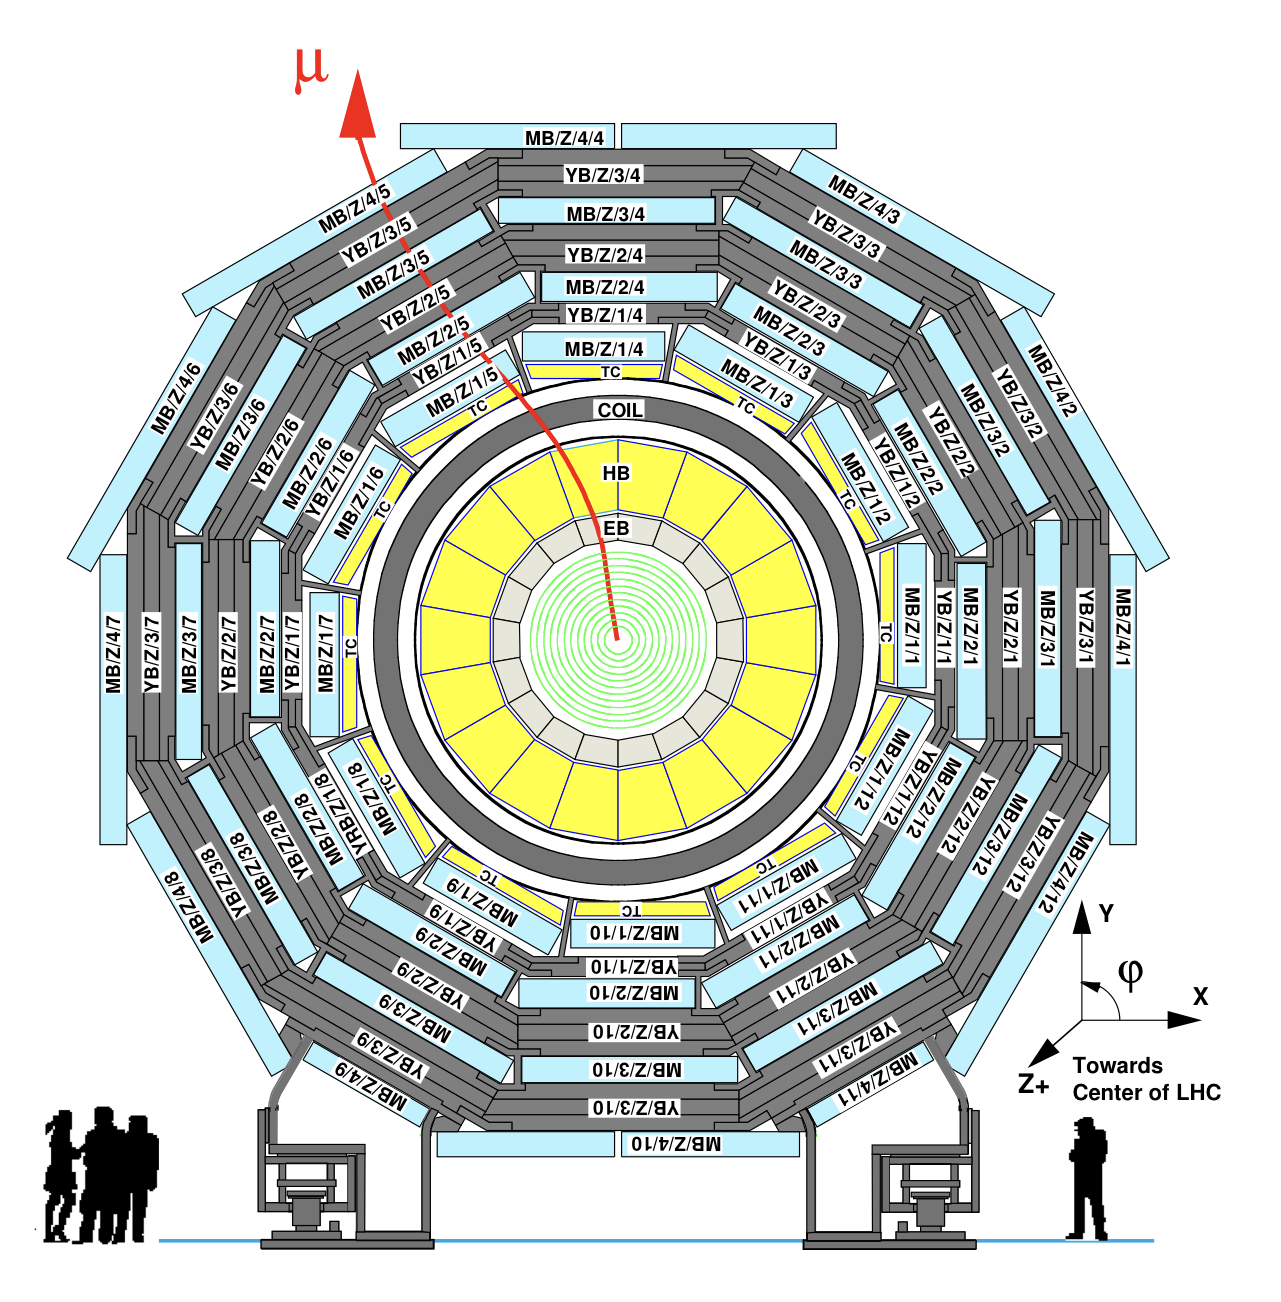
\includegraphics[width=15cm,height=10cm,keepaspectratio]{figures/cms/muonsys/drifttube_locations.jpeg}
    \caption{
        A cross section of CMS showing the locations and numbering scheme of the drift tubes in the barrel.
        }
        \label{fig:dt_locations}
\end{figure}
%%%%%%%%%%%%%%%%%%%%

\textbf{\textit{Design:}}
The first three stations contain 60 DTs each, while the station farthest from the beam pipe contains 70 DTs.
The DTs are distributed among 5 wheels, 4 stations, and 12 sectors within the muon barrel (MB) system which uses the following numbering scheme:
MB/$W$/$A$/$S$,
where $W$ is the wheel number (-2 to 2),
$A$ is the station number (1 to 4),
and $S$ is the sector number (1 to 12).
This accounts for only $5 \times 4 \times 12 = 240$ chambers, so the remaining 10 DTs are found in station 4, sectors 4 and 10, in each wheel (Fig.~\ref{fig:dt_locations}).

Each tube cross section is $13 \times 42~\mm^{2}$, within which a single anode wire is made of gold-plated stainless-steel that has a diameter of 50~\mum.
Different voltages are applied to the anode wires ($+$3600 V), electrode strips ($+$1800 V), and cathode strips ($-$1200 V).
The gas mixture within a DT is similar to that of a CSC, containing approximately 85\% Ar $+$ 15\% CO$_{2}$.

\textbf{\textit{Physics:}}
DTs are a good choice for the barrel because of the low rate and low strength of magnetic field.
Uniform drift field of 1.5 KV/cm.
A high \pt muon track will cross all 4 DT stations within the pseudorapidity range of $\abseta < 0.8$.
The reconstruction efficiency of such a track is better than 95\%.

A single SL has a time resolution of only a few nanoseconds which provides excellent bunch crossing identification.
To assist in determining muon \pt and timing, the DT system delivers the following muon track segment information to the L1 trigger:
the position of the center of gravity (to a precision of 1.5~\mm) and the corresponding angle (to a precision of 20 mrad), w.r.t. the SL reference frame.
The total resolution of a DT in $r$-$\phi$ is about 100~\mum which is comparable to the deviation caused by multiple scattering, for a muon with $\pt \le 200~\GeV$.

The gas gain is comparable to that of a CSC (about 100,000).

The maximum drift distance in a DT is 21~\mm, as can be seen in Fig.~\ref{fig:dt_cell}, which corresponds to a drift time of 380~\ns.
This value 

\subsection{Resistive Plate Chambers}
\label{subsec:rpc}

\textbf{\textit{Overview:}}
Even though CSCs~\ref{subsec:csc} and DTs~\ref{subsec:dt} cover the entire pseudorapidity range of $0 < \abseta < 2.4$, redundancy is important.
Therefore, resistive plate chambers (RPCs) are placed in both the endcaps and barrel to provide excellent timing and spatial resolution, comparable to that of scintillators, to supplement the measurements of the CSC and DT systems.
An RPC is a gaseous parallel-plate detector

RPC has better time resolution than the 25~\ns between two continguous \pp bunch crossings.

\textbf{\textit{Design:}}

Gas mixture comprised of 96.2\% C$_{2}$H_${2}$F$_{4}$ (1,1,1,2-tetrafluoroethane) $+$ 3.5\% $i$C$_{4}$H_$10$ (isobutane) $+$ 

The RPC system consists of 480 rectangular chambers that are oriented parallel to the beam pipe.
A single RPC is 2.455~\mm long 


\textbf{\textit{Physics:}}

\subsection{Gas Electron Multipliers}
\label{subsec:gem}

\textbf{\textit{Overview:}}

\textbf{\textit{Design:}}

\textbf{\textit{Physics:}}

(GEM)

Located in the forward region.
Filled with Ar/CO2 gas mixture.
The first GEMs At the time of this dissertation writing, 






% We can only assume that we produced neutrinos when momentum is apparently not conserved in an event. 
% When the protons collide at the IP they have nearly zero momentum perpendicular to the beam pipe. 
% This is called transverse momentum, because it's well... transverse to the beam pipe, the z direction.
% If we track, tag, capture all the outgoing particles and reconstruct their transverse momenta, 
% if we find out that it is NOT zero by a large amount, then we say that 

% The main purpose of the Muon System is to precisely determine the position and timing of muons.
% \begin{enumerate}
%     \item 
%     % for offline analysis.
%     \item Generate muon trigger primitives for the Level-1 trigger system.
% \end{enumerate}
% Similar to the Silicon Tracker, the Muon System doesn't try to capture the muons passing through it;
% instead it just tracks their positions. 
% In fact our very own Andrey, Guenakh, and Darin have been instrumental in implementing CSCs. 
% There's also an assembly hall downstairs where CSCs were constructed and tested 
% The  specializes muons. Au contraire; it \textit{specializes} in muon detection. 
% The Compact \textit{Muon} Solenoid would be a pretty hypocritical name if CMS did not detect muons. Au contraire; it \textit{specializes} in muon detection. 
% P
%It would be an ironic name if it did not detect muons well. 

% The Muon System is comprised of three kinds of gaseous detectors: 
% \begin{enumerate}
%     \item {\bf Drift Tubes} (DTs) found in the barrel.
%     \item {\bf Resistive Plate Chambers} (RPCs) found in both the barrel and endcap.
%     \item {\bf Cathode Strip Chambers} (CSCs) found only in the endcap.
% \end{enumerate}
% Each of these technologies is constructed differently and was designed with a specific purpose. 
% In Chapter~\ref{ch:CSC}, the inner-workings of the CSCs are explained.

% This concludes the overall design and purpose of the subdetectors that make up CMS.
% Since I have had hands-on experience working on CSCs, I will discuss the CSC components and how it works in more detail in the subsection below.

% \section{Trigger System}
\label{sec:trigger}
% TODO: Add a trigger pic.
% TODO: Add more refs.
Collection of collision data by CMS for each and every interaction under nominal LHC conditions would require 40\TB/sec, which is an insurmountable task for the CERN computing farm, whose processing is limited by CPU performance and storage capacity.
Moreover, most proton collisions at the LHC arise from soft interactions and are highly unlikely to contain signatures of new physics, meaning they are of little interest.
Hence a trigger system is designed to reduce the event collection rate to 100\KHz by rejecting uninteresting events while keeping potentially interesting ones.
CMS implements a two-stage trigger system, the first of which is the Level-1 (L1) trigger, which filters events and passes them to the High-Level Trigger (HLT).

Triggers may be prescaled for two reasons:
firstly, different physics processes are characterized by different cross sections and,
secondly, the trigger must keep up with luminosity changes.
For the former, a prescale may be used to keep large inputs under control by, for example, recording only 1 out of every $x$ collisions, where $x$ is the prescale value.
This may be implemented if a process is far more likely to be recorded in order to reduce the rate.
For the latter, it is important to note that as the luminosity drops, prescales can be relaxed and can therefore change within the same fill.
A trigger can be prescaled at both levels in the CMS trigger system.

\subsection{The Level-1 Trigger}
\label{sec:L1_trig}
The Level-1 trigger reduces the event rate from 50\MHz to 100\KHz with a latency of 3.2\mus by utilizing Field Programmable Gate Arrays (FPGAs) and Application Specific Integrated Circuits (ASICs).
The L1 trigger uses only coarsely segmented data from the calorimeters and muon detectors while maintaining all of the high-resolution data in pipeline memories in the front-end electronics.
The L1 trigger features several algorithms (L1 bits or seeds) to store a general description of the event content from events that are accepted, which is then passed to the HLT for further event processing.

\subsection{The High-Level Trigger}
\label{sec:hlt}
The HLT is a software system organized into a set of algorithms known as ``paths'' designed to select specific event topologies, thus reducing the output rate from 100\KHz to approximately 1\KHz.
Each path comprises steps (\emph{modules}) that reconstruct high-level objects and implements decisions based on their properties.
Each path can be modified by changing its modules or by defining new ones, maximizing the flexibility of the software.

The guiding principles for the construction of HLT paths are regional reconstruction (focusing only on detector regions tagged as interesting by the L1 seeds) and fast event veto (discarding uninteresting events as soon as possible to optimize trigger timing).

Selected events are stored in various Primary Datasets (PD) to be used for offline analyses.
Events with similar topologies are often found in the same PD.
Since a single event may satisfy the criteria for multple HLT paths, an event may be stored more than once in the same PD.

% % Will describe how CMS generally reconstructs objects.
% HZZ4L object selection is described in Higgs Mass chapter.
\section{Object Reconstruction}
\label{sec:obj_reco}
A single \pp collision yields thousands of particles, each of which must be identified by the CMS detector in order to be used in physics analyses.
By combining the specialized information from the various subdetectors (\eg tracks and energy clusters), particles are more confidently identified.
% The \pp collision itself is called the \emph{primary vertex} and must be carefully reconstructed (Sec.~\ref{sec:track_vertex_reco}).
Electron and photon objects are reconstructed (Sec.~\ref{sec:egamma_reco}) using the silicon tracker (Sec.~\ref{sec:tracker}) and ECAL (Sec.~\ref{sec:ecal}) systems.
The reconstruction of muon objects (Sec.~\ref{sec:muon_reco}) uses information from all subdetectors, the most important of which are the silicon tracker and muon system (Sec.~\ref{sec:muon_sys}).
Tau objects are the last kind of charged lepton to be reconstructed (Sec.~\ref{sec:tau_reco}).
Tau leptons frequently decay hadronically and so they leave hadronic energy signatures in the HCAL.
At the same time, the silicon tracker can detect a displaced secondary vertex, thanks to the relatively long lifetime of the tau lepton.
Hadronic matter is grouped into jet objects, each of which is carefully reconstructed (Sec.~\ref{sec:jet_reco}.) using information from the silicon tracker, ECAL, and HCAL (Sec.~\ref{sec:hcal}).
Finally, after accounting for all the momenta and energies of the observed particles, the missing transverse energy $\left( \MET \right)$ is evaluated (Sec.~\ref{sec:met_reco}).
This ``holistic approach'' of combining subdetector information to identify particles is called `particle-flow' (PF)~\cite{particle_flow}.

\subsection{Electron and Photon Reconstruction}
\label{sec:egamma_reco}
Electrons and photons both leave energy deposits within the crystals of the ECAL---so how are the two kinds of particles differentiated from one another?
Since photons are electrically neutral, the silion tracker will not detect them.
Another consequence of their neutrality is that photons do not bend in a magnetic field;
their energy deposits will point radially back to the vertex from which they originated.
On the other hand, electrons \emph{are} charged and so will not only be detected within the layers of the silicon tracker but will also reveal a curved track.
Hence, the energy deposits from electrons within the ECAL will \emph{not} necessarily point towards the vertex from which the electron came~\cite{Ereco_performance_2015}.

Within CMS, track fitting and pattern recognition typically occur within a single framework called the Combinatorial Track Finder (CTF), which is an extension of the Kalman filter (KF)~\cite{general_track_reco}.
However, the reconstruction of tracks of charged particles is computationally difficult.
As electrons pass through matter, they may radiate away some of their energy in the form of bremsstrahlung photons.
The distribution of this energy loss is extremely non-Gaussian and is not accurately modeled by the KF.
Instead, the CMS tracker uses a Gaussian-sum filter (GSF) algorithm~\cite{gsf} to model the energy-loss distribution as a mixture of Gaussian functions.
This ultimately improves the momentum resolution of electrons.

\subsection{Muon Reconstruction}
\label{sec:muon_reco}
Muons leave a very clean signature in the CMS detector thanks to their interactions in the muon detectors.
Consequently, muon tracks are reconstructed by dedicated algorithms that are independent from the iterative PF identification system used to reconstruct other particles.
These algorithms are based on a KF method that accounts for muon energy loss in the detector materials.

The most reliable muon detection occurs when both the silicon tracker \emph{and} the muon system both register hits corresponding to the same particle object.
When both subsystems detect such a particle---\emph{most likely a muon}---it is called a `global muon'.
This can be compared to the situation when only the muon system registers hits, in which case this is most likely a `standalone muon' and must be rejected due to its worse momentum resolution and higher contamination from cosmic ray backgrounds.
The opposite case occurs when only the tracker registers hits and the corresponding particle is termed a `tracker muon'~\cite{reco_muon}.

The tracker and muon systems exhibit high reconstruction efficiency, and about 99\% of muons are reconstructed either as tracker or global muons.
Candidates sharing the same inner tracks are merged into a single object.
Muon charge and momentum assignments are calculated from tracker measurements for muons with $\pT < 200\GeV$, since multiple scattering may degrade the muon detector measurements.
The global track curvature is instead used for muons with $\pT > 200\GeV$ if the charge-to-momentum ratio agrees within two standard deviations from the tracker-only measurement.
The muon transverse momentum resolution ranges from 1--6\% depending on the $\eta$ coordinate for muons with $\pT < 100\GeV$, which is better than the 10\% resolution for central muons with $\pT \approx 1\TeV$.

\subsection{Tau Reconstruction}
\label{sec:tau_reco}
Tau leptons are characterized by a mean lifetime of about $2.9 \times \tentotheminus{13}\snd$, meaning they decay within a few millimeters from their production point for the typical Lorentz boosts at the LHC.
Fully leptonic decays are reconstructed in a similar way as other leptons, semileptonic decays to hadrons ($\tau_\text{h}$) and a neutrino result in small and collimated hadron jets requiring a specific reconstruction algorithm.
The $\tau_\text{h}$ reconstruction algorithm should be able to determine the $\tau$ decay mode, identify PF candidates associated with both charged hadrons and photons from $\pi^0 \rightarrow \gamma\gamma$ decays, and regroup them together to estimate the $\tau_\text{h}$ kinematic properties.
The hadrons plus strips (HPS) algorithm~\cite{hps_algo1, hps_algo2} analyzes PF candidates and assesses their compatibility with $\tau_\text{h}$ objects.
Contributions from neutral pions can appear either directly as photon PF candidates or as electron candidates clustered inside the jet.
Therefore these candidates with $\pT > 0.5\GeV$ are clustered into `strips' using an iterative procedure.
A dynamic strip construction was introduced in Run 2 and defined the $\Delta\eta$ and $\Delta\phi$ clustering window sizes as functions of the strip \pT to ensure an optimal collection of the energy and to minimize the impact of background.

\subsection{Jet Reconstruction}
\label{sec:jet_reco}
Quarks and gluons undergo a hadronization process, requiring the recollection and measurement of the hadronization products in order to estimate their initial momentum.
Jets resulting from this process are reconstructed by clustering the PF candidates with the anti-\kt algorithm~\cite{Cacciari:2008gp, Cacciari:2011ma},
which combines candidates that are close to each other based on a metric that is defined to produce jets of an approximate conic shape clustered around the hardest particles in the event.
The size of the jet cone is determined by the distance parameter $\Delta R$ at which the algorithm is operated (typically $\Delta R = 0.4$ and $ \Delta R = 0.8$).
The anti-\kt algorithm is resilient against infrared and collinear events, \ie it is not affected by soft radiation or collinear parton splitting. 

The jet four-momentum is calculated as the vector sum of the four-momenta of the clustered candidates and a set of corrections are applied to calibrate the jet response using the information of particles generated in a simulation.
These corrections of the jet energy scale take into account the contribution of the pileup in the event, nonlinearities in the detector response to hadrons, and residual differences between the data and simulation used during calibration.
Corrections are validated using dijet, multijet, $\gamma + \text{jets}$, and leptonic $\PZ + \text{jets}$ events~\cite{CMS:2016lmd}.
Typical jet resolutions are about 15--20\% for jets at 30\GeV, 10\% at 100\GeV, and 5\% at 1\TeV.

\subsection{MET Reconstruction}
\label{sec:met_reco}
Although neutrinos are undetectable final state particles, their presence can be indirectly inferred by an imbalance in the vector sum of the total transverse momentum.
The negative projection of this vector onto the transverse plane is denoted as missing transverse momentum, \ptvecmiss, and its magnitude is typically called the missing transverse energy (MET).

A bias can be introduced into the \ptvecmiss determination through inefficiencies within the tracking algorithm, minimal thresholds in the calorimeter energy estimation, and nonlinearities of the energy response for hadronic particles within the calorimeters.
Thus, a correction is applied by propagating the jet energy corrections $\left( \vec{p}_{\text{T}, j}^{\kern1pt \text{corr}} - \vec{p}_{\text{T}, j} \right) \equiv \Delta \vec{p}_{\text{T}, j}$ for each jet $j$ out of all $N_\text{jets}$ jets into the calculation:
\begin{equation}
\ptvec^{\kern1pt \text{miss,corr}} =
    \ptvecmiss - \sum^{N_\text{jets}}_{j}
        \left( \Delta \vec{p}_{\text{T}, j} \right).
\end{equation}
If a muon is identified within the jet cone, its four-momentum is subtracted from the jet momentum when computing the correction and then added back into the \ptvecmiss sum.
%%%%%%%%%%%%%%%%%%%%%%%%%%%%%%%%
%--- Higgs Mass Measurement ---%
%%%%%%%%%%%%%%%%%%%%%%%%%%%%%%%%
% \chapter{HIGGS BOSON MASS MEASUREMENT IN THE \texorpdfstring{\hzzfourl}{H to ZZ to 4l} CHANNEL}
\label{ch:higgs_mass}
% Need to use \texorpdfstring{} so it also shows in pdf bookmarks.
\section{Motivation}
\label{sec:higgs_motivation}
When the CMS and ATLAS collaborations announced the discovery of the Higgs boson on July 4, 2012,
% TODO: Add higgs production modes here?
% TODO: Include ref to HIG-21-019 somewhere around here?
this was a momentous achievement in particle physics because the so-called ``missing'' piece of the SM was found~\cite{chatrchyan_observation_2012, aad_observation_2012, chatrchyan_observation_2013}.
Evidence of the Higgs boson's existence also motivates the associated Higgs field, which permeates all of spacetime and explains the origins of the masses of all the other massive fundamental particles (Chapter~\ref{ch:theory}).

The Higgs boson is interesting for a variety of reasons.
First, it is currently one of a kind---the only fundamental scalar particle ever discovered at the time of this writing.
Second, the mass of the Higgs boson theoretically determines the stability of our very Universe (Fig.~\ref{fig:universe_stability}).
Third, the unique boson could be a portal to new physics---\ie physics beyond the Standard Model (BSM)---\eg by decaying into BSM low-mass dilepton mass resonances (Chapter~\ref{ch:dilep_res}).
Fourth, the Higgs boson may not be the only one of its kind; some BSM models theorize that other kinds of Higgs bosons may exist~cite{Branco:2011iw}.
Fifth, \emph{are we certain that the Higgs boson discovered in 2012 is the same as the one predicted by the SM?}
To check this, it is necessary to compare the Higgs boson's measured properties to its predicted ones.
One such property is the mass of the Higgs boson $\left( \mH \right)$.

Although many previous measurements of \mH have already been made (\eg by the ATLAS and CMS collaborations as shown in Fig.~\ref{fig:atlas_cms_mH_meas}), this chapter presents a recipe for the measurement of \mH that is predicted to give the world's most precise value of \mH to date, once the data are unblinded.
%=== ATLAS and CMS measurements of mH.
%%%%%%%%%%%%%%%%%%%%
\begin{multiFigure}
    \centering
    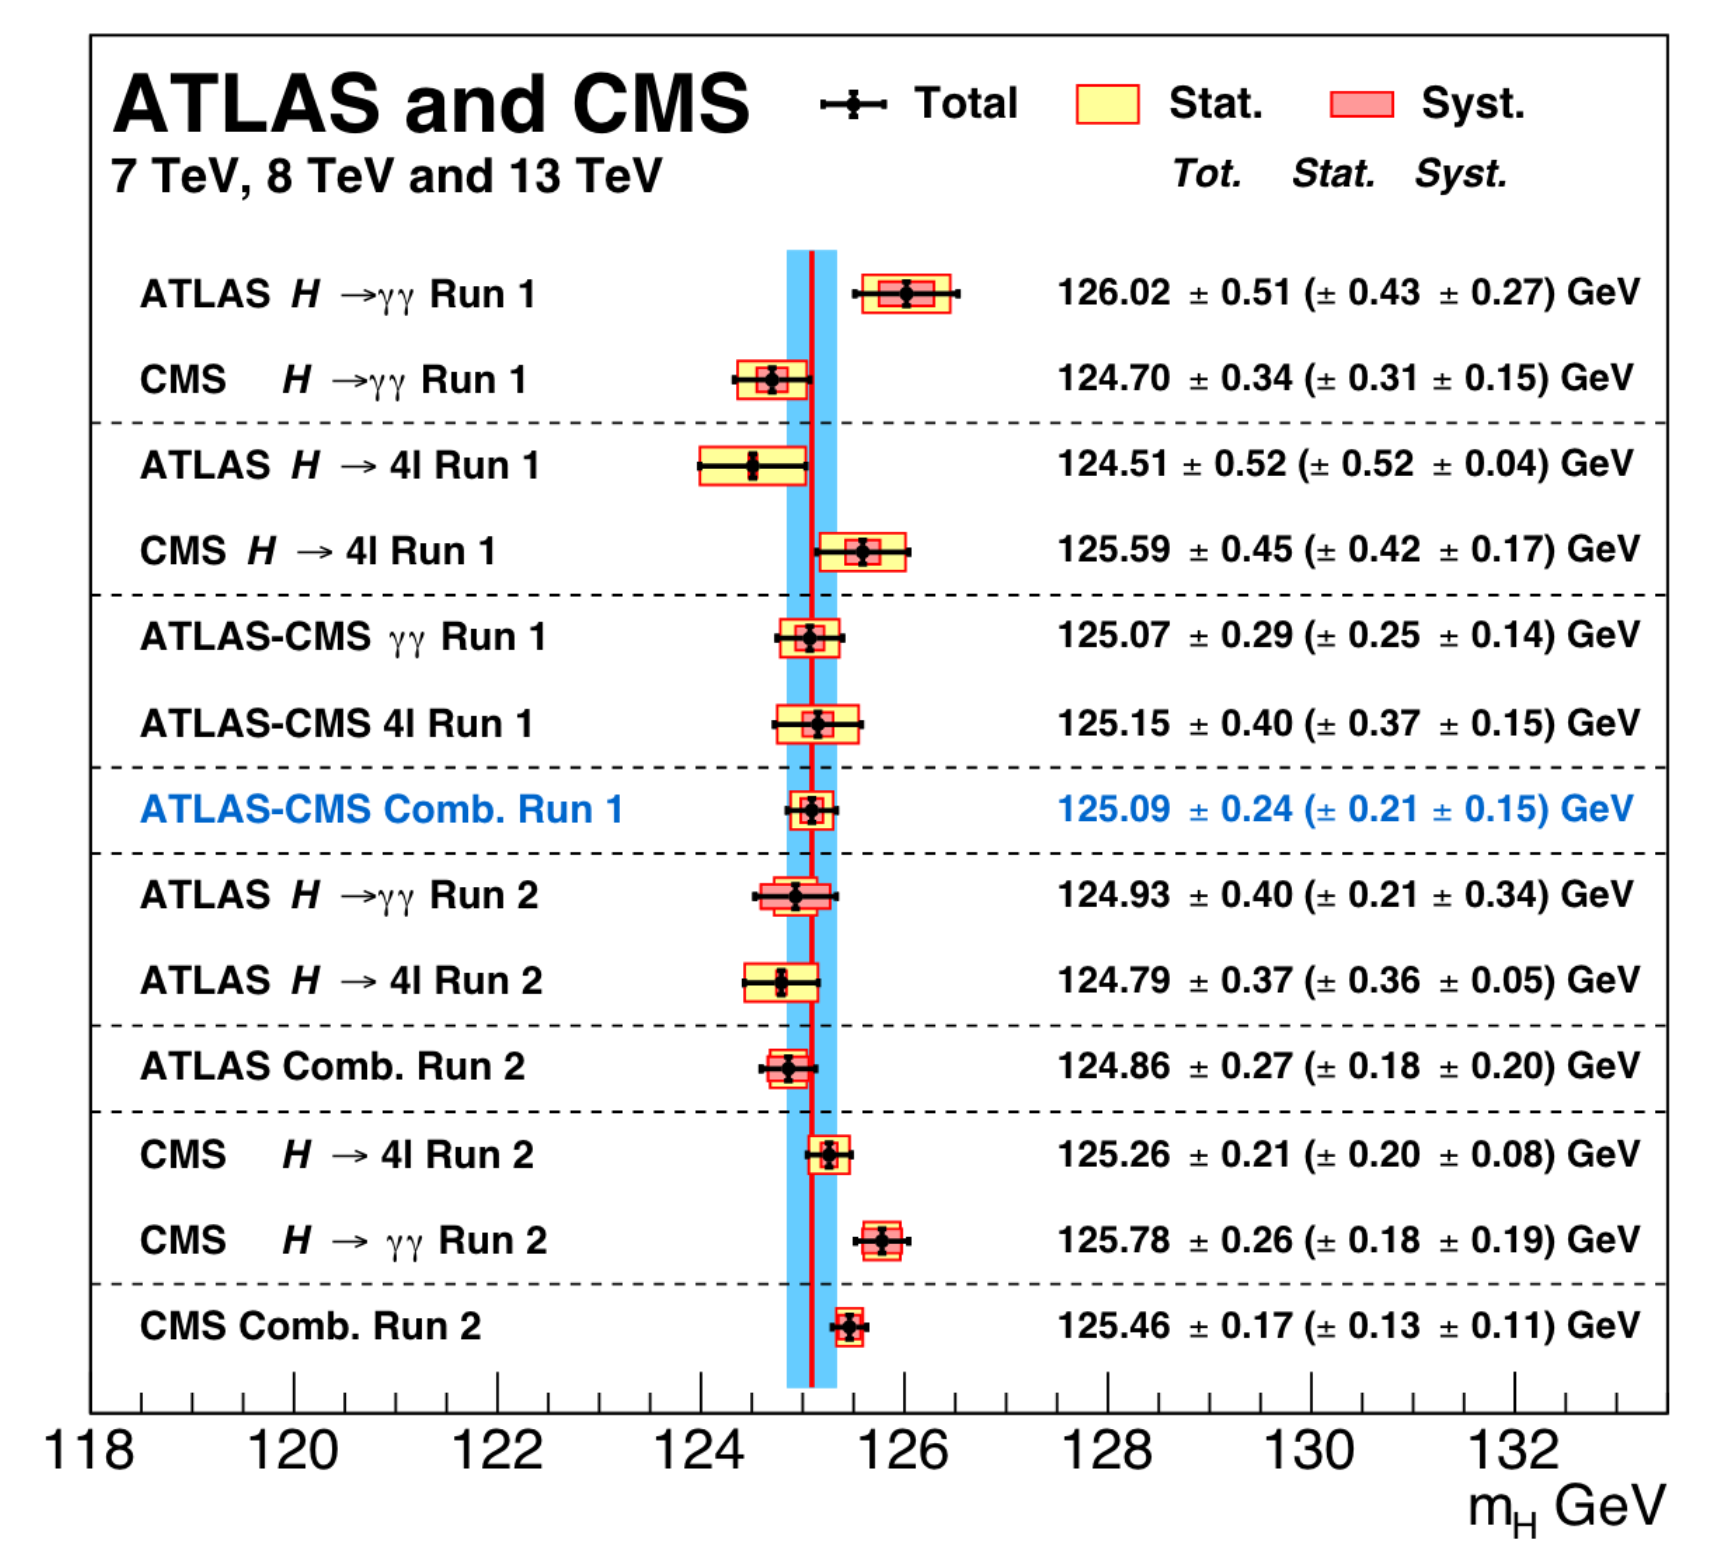
\includegraphics[width=\textwidth,keepaspectratio]{figures/higgsmassmeas/all_mH_measurements_atlas_cms.png}
    \captionof{figure}
        [Various measurements of \mH made by the CMS and ATLAS collaborations]
        {Various measurements of \mH made by the CMS and ATLAS collaborations in the \htoyy and \hzzfourl channels, during Runs 1 and 2 of the LHC.
        Plot taken from~\cite{particle_data_group_review_2020}.}
    \label{fig:atlas_cms_mH_meas}
\end{multiFigure}
%%%%%%%%%%%%%%%%%%%%
% Some properties of the Higgs boson can be predicted by the SM, like 
%     - There are many results on Higgs properties: spin, charge, decay processes, lifetime, mass.
%     - The last of these is the focus of this dissertation and is of particular importance to the Universe: depending on mH and mtop, the stability of the Universe.
% - Why this thesis is important:
%     - This thesis describes the methodology and results of the best precision measurement of mH to date by using the hZZ4l decay and Full Run 2 data set from CMS.
%     - Run 2 provides more data -> more precision on measurements of Higgs properties.
%     - In addition to more HZZ4l events, this analysis provides new techniques, specifically the VX constraint.
%     - Predict mH for Run 3, will start soon summer 2022 and provide an approximate 300? /fb of L int.
%     - In 2026(?), HLLHC provides even more data. ref snowmass paper.
The estimate for the lowest uncertainties on \mH comes from the following improvements compared to previous measurements:
\begin{itemize}
    % More data.
    \item Nearly four times as much collected data from Run 2 $\left( \lumiint = \lumiruntwo \right)$ \vs the data used for the 2016 measurement $\left( \lumiint = \lumisixteen \right)$.
    % Four final states (instead of three).
    \item Four final-state categories: \fourmu, \foure, \twoetwomu, \twomutwoe.
    In previous measurements, the last two final states (the mixed-flavor states) were combined, when truly they have different kinematical properties (depending on into which lepton pair the \Zone decayed):
    different peak widths (instrumental resolutions), different signal efficiencies, and different relative levels of reducible background.
    % Using UL reco (better electron pT resolution).
    \item Ultra-Legacy (UL) reconstruction for muon, electron, photon, and jet tracks.
    This signficantly improves electron momenta and improves the other particle momenta, though to a lesser degree.
    % Vertex constraint.
    \item The measurements of muon \pt are improved by constraining the muon tracks to originate from the interaction vertex (also called a \emph{vertex+beamspot constraint}).
    \item When extracting the value of \mH in past measurements, a 3D $\text{pdf} \left( \mfourl, \mfourlerr, \Dkinbkg \right)$ was built into a factorized form
    $f \left( \mfourl, \mfourlerr \middlepipe \mH \right)   \cdot   g\left( \Dkinbkg \middlepipe \mfourl \right)$,
    which was later found to contain an existing correlation between \mfourlerr and \Dkinbkg.
    To account for this correlation, now the events are split into 9 categories based on the per-event \emph{relative} mass uncertainty $\left( \relmfourlerr \right)$ and, for each, a 2D $\text{pdf} \left( \mfourl, \Dkinbkg \middlepipe \mh \right)$ is built.
    % Z1 mass constraint.
    % The improvement here is that now the muon tracks are constrained to come from the interaction vertex in the fit (sometimes called a \emph{vertex constraint}).
    \item The systematic uncertainties on electron and muon momentum scales $\left( \pt^{\Pe, \mu} \right)$ are reduced, thanks to a more detailed analysis on the uncertainties.
    This has the additional effect of significantly reducing the uncertainty on the per-event four-lepton mass resolution.
\end{itemize}

The layout of the remainder of this chapter is as follows:
First, a general overview of the logic and analysis workflow for the \mH measurement is motivated in Sec.~\ref{sec:analysis_overview}.
The specific data sets, simulated samples, and triggers used in the analysis are then detailed in Sec.~\ref{sec:analyzed_data}.
Then the event reconstruction and event selection are described in Sec.~\ref{sec:evt_sel}.
Afterwards, an analysis of the background estimation is given in Sec.~\ref{sec:bkg_estim}.
The signal modeling and improvements utilized in this measurement are then laid out, which include the kinematic discriminant, per-event mass uncertainties, and the vertex constraint in Sec.~\ref{sec:signal_model}.
A treatment of the systematic uncertainties follows in Sec.~\ref{sec:syst_uncert}.
The chapter concludes with the expected uncertainties on the \mH measurement in Sec.~\ref{sec:results}, considering Full Run 2 data from the LHC.

% \begin{itemize}                                                                          
%     \item Sec.~\ref{sec:analysis_overview}: General overview of the analysis of the Higgs boson mass measurement.
%     \item Sec.~\ref{sec:analyzed_data}: Data sets, triggers, and simulation.
%     \item Sec.~\ref{sec:evt_sel}: Event reconstruction and selection.
%     \item Sec.~\ref{sec:bkg_estim}: Background estimation.
%     \item Sec.~\ref{sec:signal_model}: Signal modeling and improvements, including kinematic discriminant, per-event mass uncertainties, VXBS constraint, reference to ad hoc studies in appendix.
%     % \item Observables: Four-Lepton Invariant Mass, Per-Event Mass Uncertainty, Matrix Element-Based Kinematic Discriminant) (Sec.~\ref{sec:observables})
%     \item Sec.~\ref{sec:syst_uncert}: Systematic uncertainties.
%     \item Sec.~\ref{sec:results}: Results.
% \end{itemize}

\section{Analysis Overview}
\label{sec:analysis_overview}
The first step to performing a precision measurement of the Higgs boson mass (\mH) is to ``observe'' many Higgs bosons.
However, production of a Higgs boson is essentially nonexistent in everyday conditions and is still extremely rare even in the high-energy \pp collisions of the LHC.
At a center-of-mass energy of 13\TeV, the total inclusive inelastic cross section of two protons colliding is 70\mb TODO: CITE.
Comparing this to the production cross section of a Higgs boson (TODO sigma(pptoH) = 59 pb) shows that a Higgs boson is produced in approximately one out of every billion \pp collisions.  TODO CITE

To complicate matters further, the Higgs boson has a \emph{very} short mean lifetime of only $1.6 \tentotheminus{22}\snd$~\cite{pdg}.
Thus, the Higgs boson is not directly detected by CMS but is instead \emph{inferred} from its stable decay products that enter the various subdetectors.
Among all the fundamental particles so far discovered, the Higgs boson bears the second heaviest mass (approximately 125\GeV), the first belonging to the top quark (Section~\ref{sec:sm}).
This gives the scalar boson sufficient energy to decay into at least 9 different final states.
\textcolor{red}{MENTION THAT NOT ALL DECAYS MAKE ON-SHELL PARTICLES?}
Each decay occurs with a different probability---the \emph{branching fraction} or \emph{branching ratio} (\br)---whose value depends on \mH as shown in Fig.~\ref{fig:higgs_br}.
\begin{figure}[!htbp]
    \begin{center}
        % Figures come from:
        % https://twiki.cern.ch/twiki/bin/view/LHCPhysics/LHCHWG?redirectedfrom=LHCPhysics.LHCHXSWG#Higgs_cross_sections_and_decay_b
		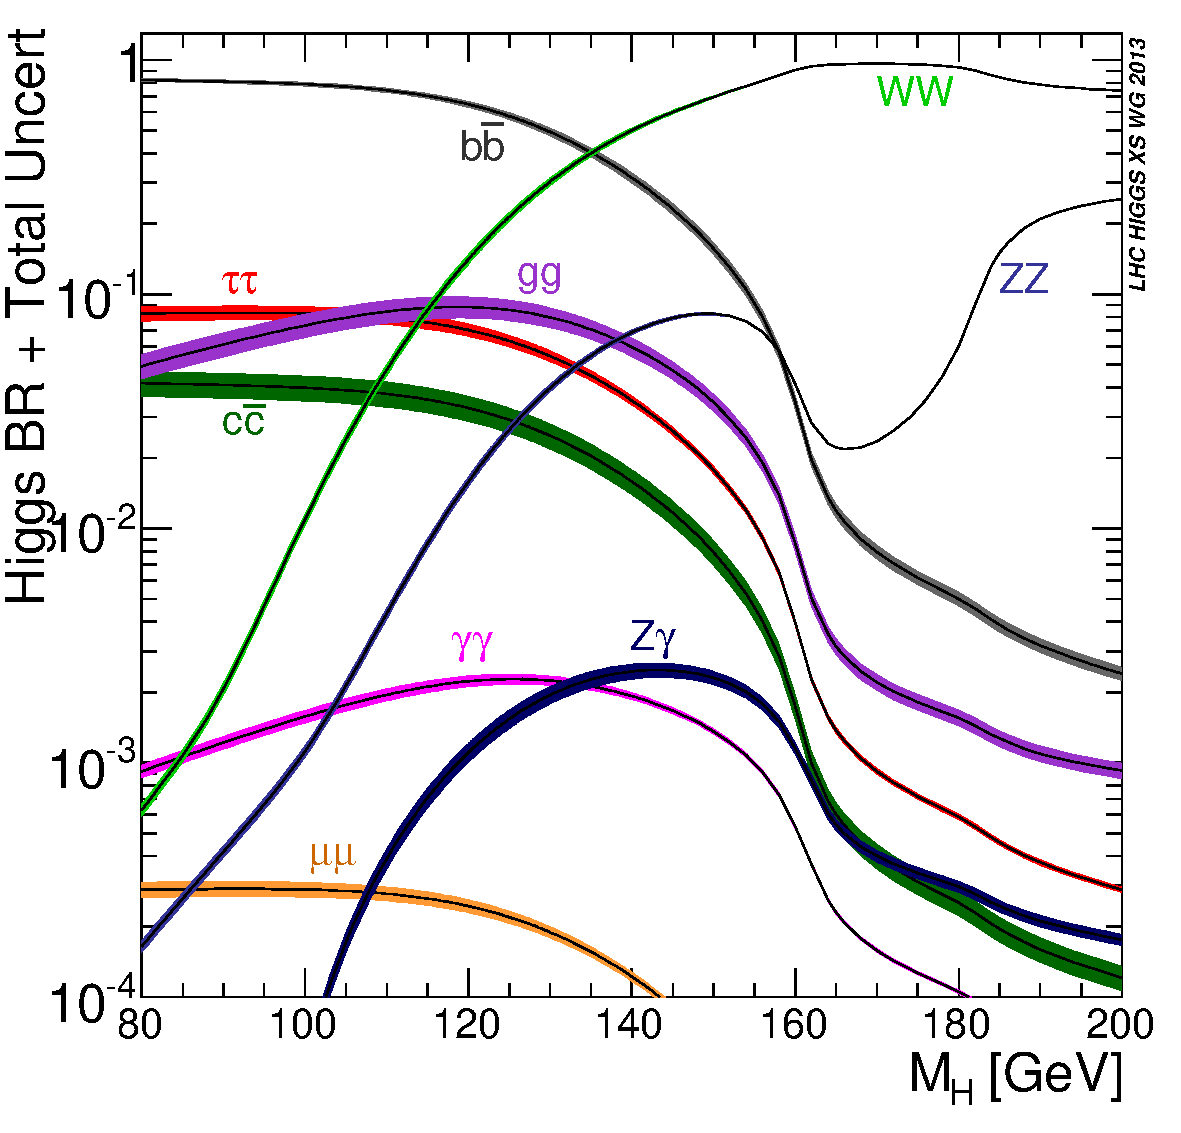
\includegraphics[width=0.48\textwidth]{figures/higgsmassmeas/higgs_BR_80to200GeV.pdf}
		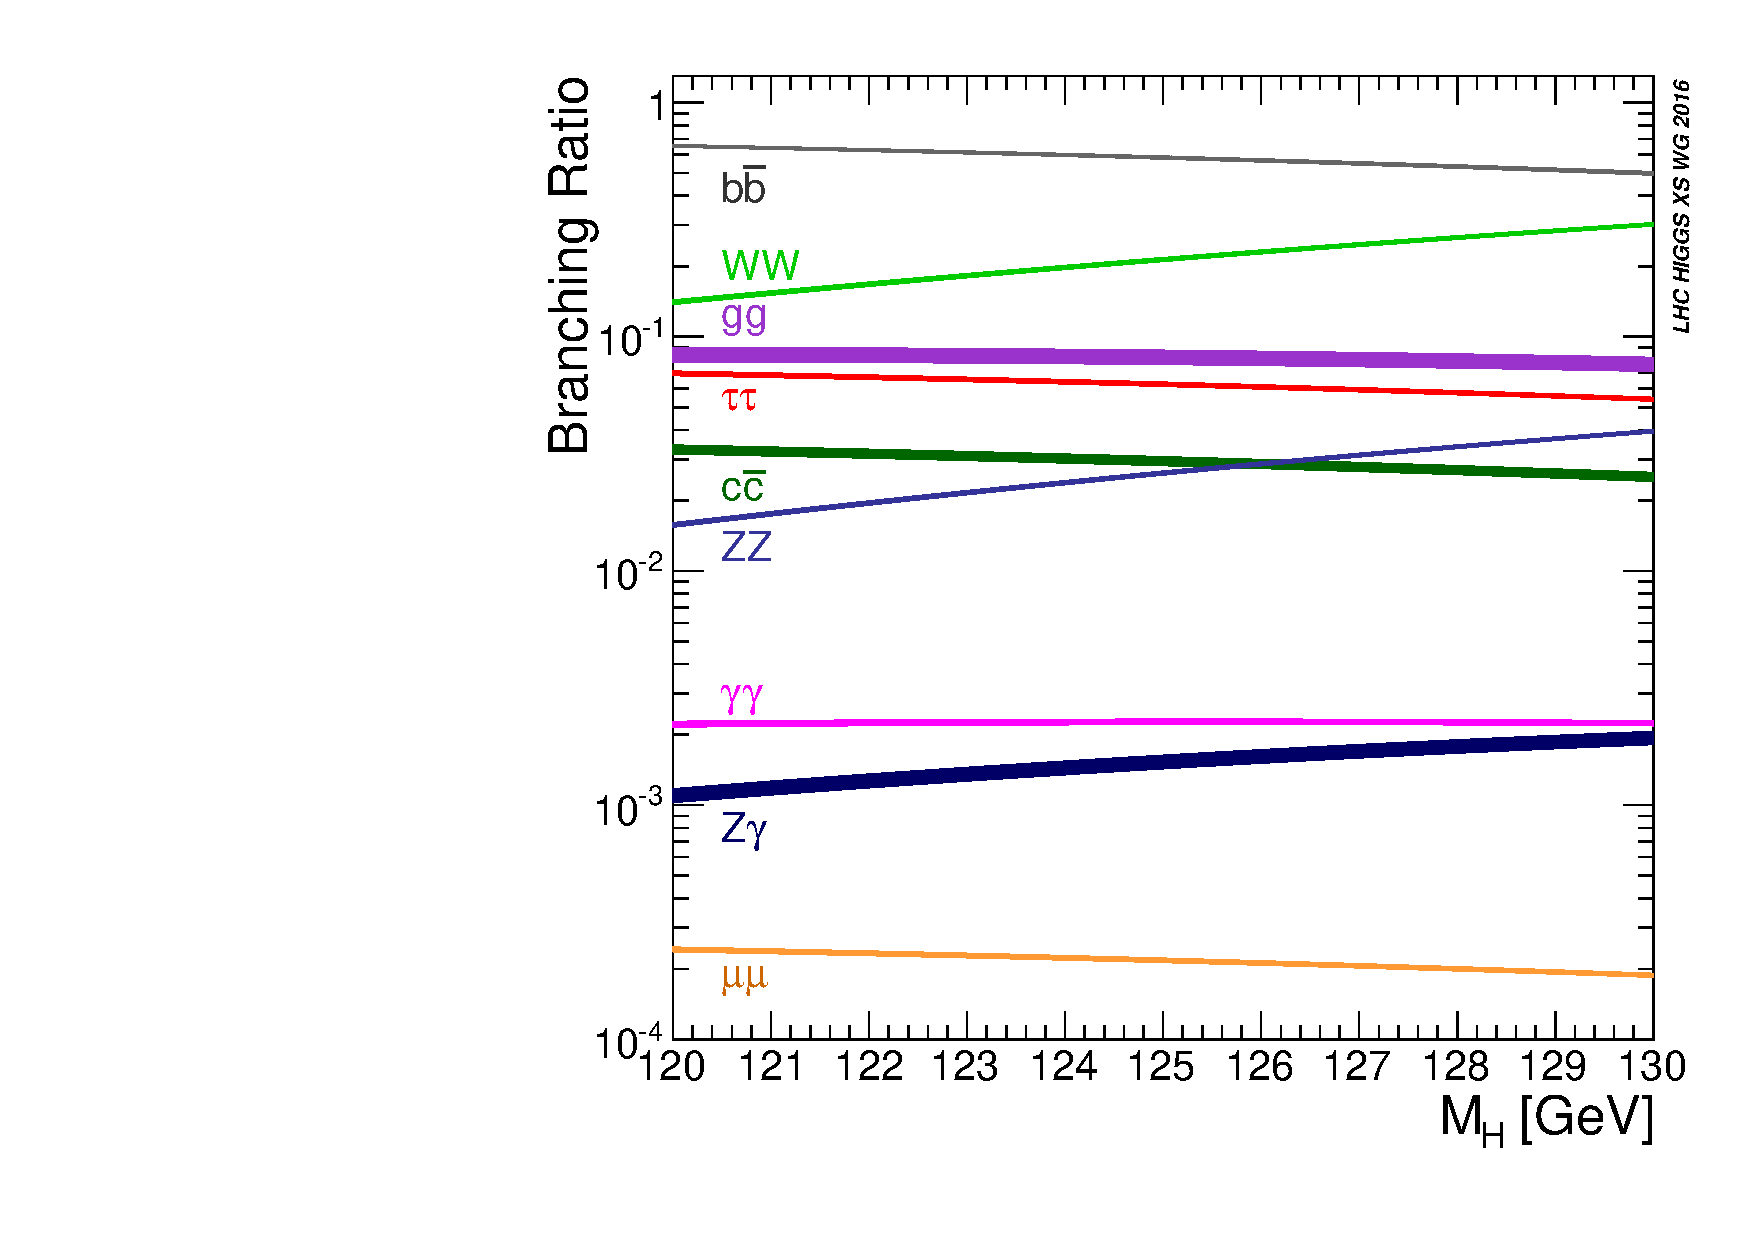
\includegraphics[width=0.48\textwidth]{figures/higgsmassmeas/higgs_BR_120to130GeV.pdf}
		\caption{
            The branching ratios of various Higgs boson decays as a function of the Higgs boson mass
            over a wide range (Left) and a narrow range (Right) of values.
            }
		\label{fig:higgs_br}
	\end{center}
\end{figure} 
The question then becomes, \emph{``Which Higgs boson decay mode is most useful for the measurement of \mH?''}.
% Real particles enter detectors in CMS which send signals to various electronics.
% Particle Flow algorithm pieces the information together to construct objects out of each event.
% Now, instead of just a deposit of energy in the ECAL and corresponding hits in the silicon tracker, the particle is identified as a newly produced electron.
% CMS records which kinds of objects came from which events and stores the information in \emph{data sets} (TODO: ref Section future).

Owing to its large signal-to-background ratio of approximately 2 and its relatively rare four-lepton final state, the \hzzfourl decay channel is chosen and is called the \emph{signal} process.
On average, a Higgs boson will decay into two \PZ bosons (one on-shell and one off-shell) only 2.6\% of the time.
In turn, each \PZ boson \emph{may} decay into two opposite-sign, same flavor (OSSF) leptons (\Ztolplm, where $\ell = \Pe, \mu$) on average approximately 6.7\% of the time.
This signal process then gives rise to four distinct final states: \foure, \fourmu, \twoetwomu, \twomutwoe.
The branching ratio for the overall signal process is then calculated as: % B(Z->ee)=0.033632, B(Z->mumu)=0.033662
\begin{equation*}
    \BRof{\hzzfourl} = \BRof{\htozz} \left[ \BRof{\Ztolplm} \right]^2 = 1.8\tentotheminus{3}.
\end{equation*}
Thus, a signal event is expected to be produced only once in about every \emph{trillion} \pp collisions.

The strategy is then to search the \pp collision data collected and analyzed by the CMS detector (Chapter~\ref{ch:cms_detector}) for all the detected \hzzfourl events.
The task is not so straightforward;
events in the data are categorized---not by the entire decay process---but by their final state, based on which triggers fired to collect which events.
Section~\ref{sec:datasets_simul_trig} describes the triggers used for this analysis to select events with the \fourl final state found in the corresponding data sets.
For each chosen event, the subdetectors of CMS (Chapter~\ref{ch:cms_detector}) provide a plethora of track and energy-detection information to reconstruct \emph{objects}---representations of the underlying particles within the event.
The reconstructed objects are then assembled in a fashion that checks if the logic coincides with the process of interest: \hzzfourl.  % TODO: Clean up this sentence.
For example, a pair of OSSF lepton-like objects should appear to come from a \PZ-like object---\ie having a nominal mass of approximately 91\GeV and zero net electric charge---instead of, say, appearing to come from a \PH-like object.
Two such \PZ-like objects must be formed and should appear to come from a \PH-like object.
% OSSF-dilepton objects should each appear to come from a \PZ-boson-like object (\eg having a nominal mass of approximately 91\GeV and zero net electric charge)---instead of, say, coming from a Higgs-boson-like object.
All throughout, the reconstructed event must obey physics conservation laws (energy, momentum, charge, \etc) and the associated objects may even be required to pass certain detector selection criteria (\eg $\pt^\mu > 5\GeV$).
% This process hinges on the conservation of momentum, since in the longitudinal ($z$) direction the \pp collision has initial and final.
% Specifically, the 
%     - The \PZ boson has a precisely measured mass of TODO a neutral particle, so the two leptons into which it decays should combine to Group two leptons together, 
%     - Form two different pairs of opposite-sign, same-flavor (OSSF) leptons
%     - If it appears that the to select specific hzz4l events (\emph{event selection}).
These criteria are analysis-specific and are collectively called the \emph{event selection} of the analysis.
The event selection for this analysis is described in Section~\ref{sec:evt_sel}.  % TODO: ref may be wrong.

Although the event selection is constructed to select only signal events, it is not guaranteed;
there are certain physics process that have exactly the same initial and final states as the signal process.
Such processes ``contaminate'' the collected signal events and are called \emph{background processes}.
Fig.~\ref{TODO} shows how identical initial state gluons can react to produce exactly the same final state particles, while producing different intermediate particles:
the signal process (Left), initiated by gluon-gluon fusion \vs a background process (Right) which skips the intermediate Higgs boson.
It is imperative for all physics analyses to maximize the number of collected signal events while minimizing the number of collected background events.
Section~\ref{sec:bkg_estim} discusses the associated background processes and how to estimate the number of events these contribute to the signal region.
\begin{figure}[!htbp]
	\begin{center}
		
\includegraphics[width=0.48\textwidth]{figures/placeholder.png}  % TODO.
		
\includegraphics[width=0.48\textwidth]{figures/placeholder.png}  % TODO.
		\caption{
            Feynman diagrams showing how the initial and final states are the same
            for the signal process (\gghzzfourl, Left) and one possible background process (\ggzzfourl, Right).
        }
		\label{fig:feyndiag_sig_vs_bkg}
	\end{center}
\end{figure}

Before drawing conclusions from the data themselves, it is necessary for particle physicists to make predictions about their analysis using simulated events or \emph{simulation}.
These events simulate a specific process (\eg $\pp \to \hzzfourl$), governed by some theoretical framework that is programmed mathematically into the software package.
% events from simulated particle physics collisions--- are created by software physicists have created software packages that simulate particle physics collisions,
% the resulting particle transformations using various theoretical frameworks,
% and even the interactions that particles have with the virtual detectors, through which they traverse.
Programs like \MGvATNLO and \POWHEG can simulate millions of rare (or even \emph{fictitious}) events, which might otherwise take many years to observe in data.
Furthermore, software can even simulate the particles as they travel through the simulated detectors.
Programs like \GEANTfour show analysts what to expect as the particles interact with a virtual version of the CMS detector.
Predictions from simulation can then be compared to the truth---the data---as a way to check the accuracy of the analysis.
For example, a surplus of events in data where none was expected may lead to the discovery of new particles, as was the case for the discovery of the Higgs boson.
% agreement or deviations in what was expected.
The simulated events for this analysis are described in Section~\ref{sec:datasets_simul_trig}.

So how is the measurement of \mH obtained?
Since the signal process is \hzzfourl, conservation of energy leads one to expect that $\mfourl \approx \mH$.
Although this is not how the final measurement is obtained, it is a logical starting point.
The distribution of \mfourl values reveals that the Higgs boson mass resonance stands well above the distribution of expected background events (Figure~\ref{fig:m4l_run2}).
Simulated signal events are then used to predict the \emph{line shape} of this signal peak (Section~\ref{sec:signal_model}).
This signal modeling is performed using a double-sided Crystal Ball function to fit the line shape, for various mass points of \mH, in each of the four final states.
% m4l dist Full Run 2.
%%%%%%%%%%%%%%%%%%%%
\begin{figure}[pbth]
    \centering
    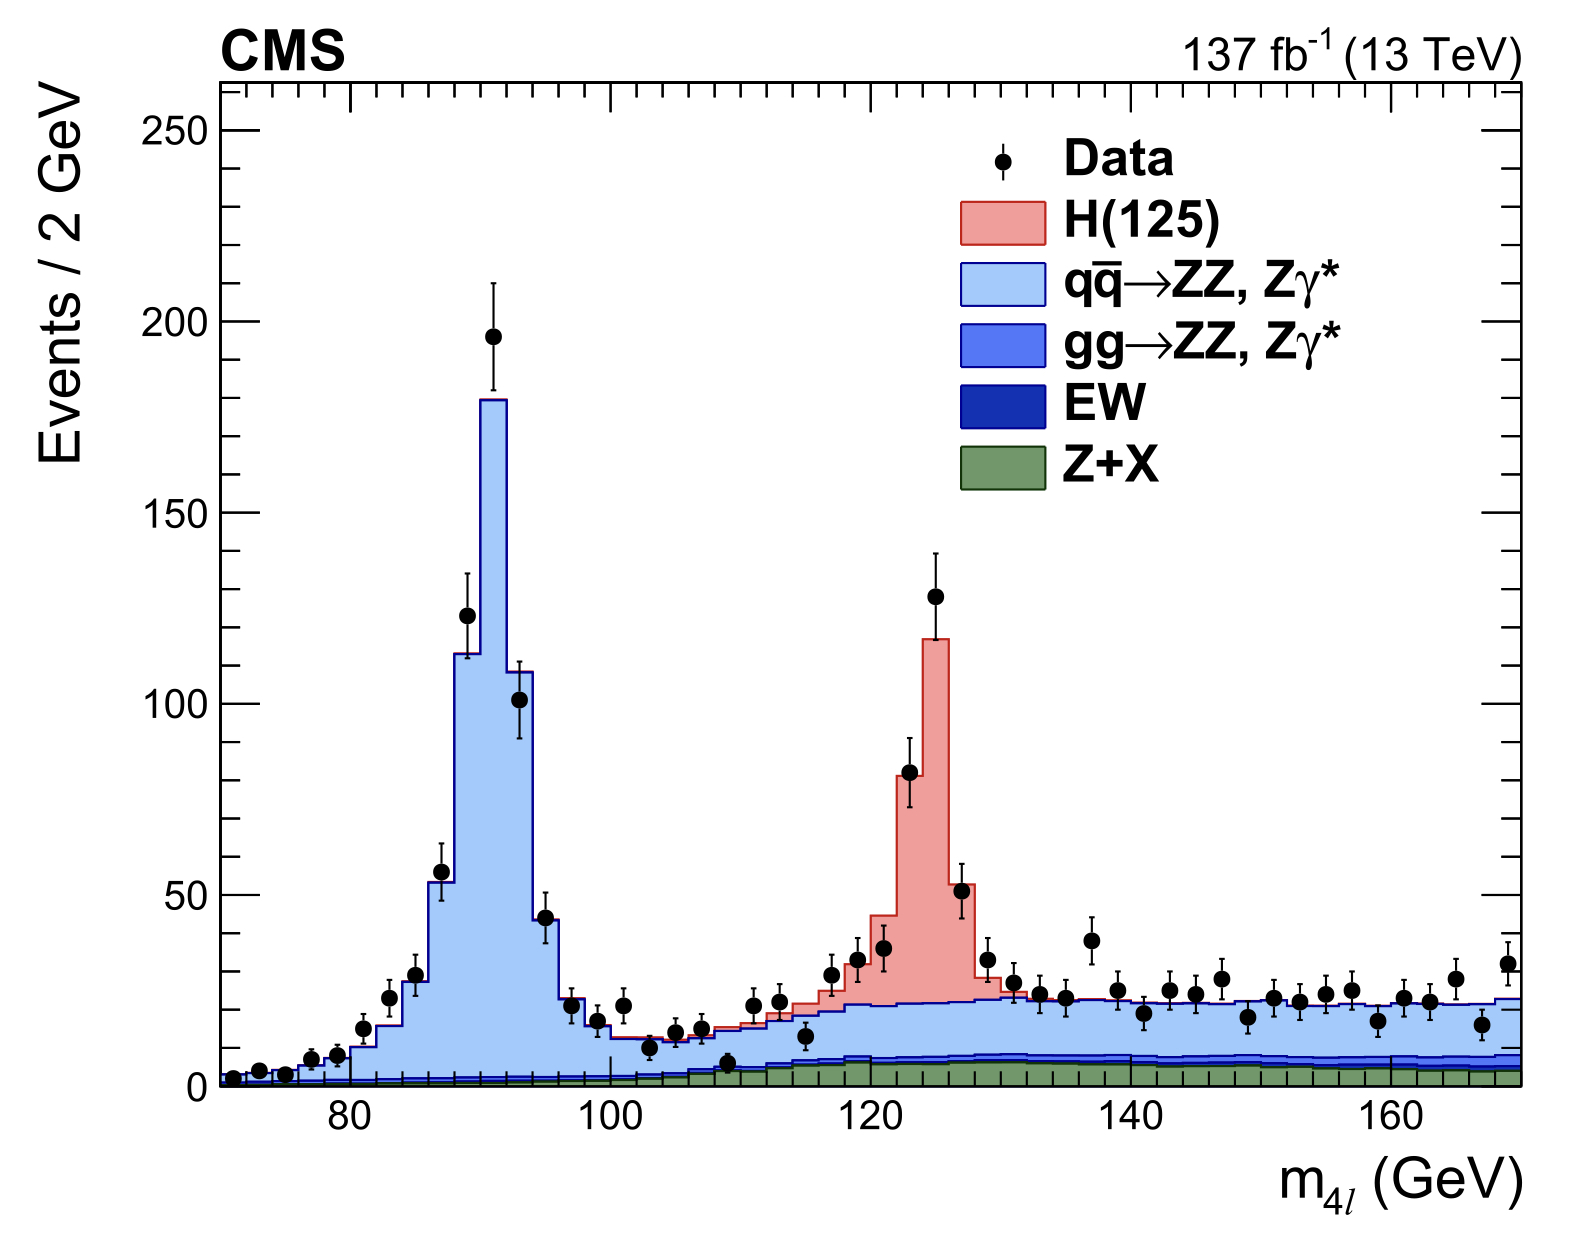
\includegraphics[width=10cm,height=10cm,keepaspectratio]{figures/higgsmassmeas/m4l_FullRun2_epjc.jpeg}
        \caption{Distribution of \mfourl from \hzzfourl events using Full Run 2 data.}
        \label{fig:m4l_run2}
\end{figure}

The precision of the measurement of \mH is improved by implementing several techniques:
calculating a per-event matrix element kinematic discriminant,
deriving correction factors for \mfourl uncertainty for various regions of phase space,
reevaluating the lepton \pt values using a \Zone mass constraint,
and constraining the four muon tracks to the selected vertex (\emph{vertex constraint}).
The implementation of these techniques is discussed in Section~\ref{sec:techniques}.
% The first technique is called the \Zone mass constraint, which uses the benefit of the mostly on-shell \Zone mass resonance to reevaluate the momenta of the two leptons that built the \Zone, on a per-event basis.
% This improves the overall lepton momentum resolution, thereby improving the resolution of the \mH peak.
% The second technique is per-event mass uncertainty.
% The third technique is vertex constraint.

% is mostly on-shell as opposed to the \Ztwo.
% Z1 significantly on-shell, but Z2 is mostly off-shell.
% 	- Therefore just perform constraint on mZ1.
% 	- Idea is to reevaluate the lepton
% - Per-event 

Important in any scientific analysis is the careful study of all the associated uncertainties that inherently come with making \emph{any} measurement.
The two main kinds of uncertainties are either \emph{statistical}, which depend on the number of data points used to the make the measurement, or \emph{systematic}, which depend on the instrumentation precision used to make the measurement.
The systematic uncertainties for this analysis include:
\begin{itemize}
	\item \lumiint (TODO 2.5\%)
	\item Lepton identification and reconstruction efficiencies (TODO 2.5--9\%): lepton energy scale
	\item BOTH OF THE ABOVE AFFECT SIGNAL AND BKG
	\item Estimation of the reducible background.
\end{itemize}
The systematic theoretical uncertainties include:
\begin{itemize}
	\item renormalization and factorization scale uncertainties
	\item choice of the set of parton distribution functions
	\item BOTH OF THE ABOVE AFFECT SIGNAL AND BKG
	\item branching fraction uncertainties for signal and background processes.
\end{itemize}
These uncertainties are discussed in Section~\ref{sec:syst_uncert}.

The resolution of the peak 
Ways to improve the 
Do likelihood fit.

\textbf{FROM THE AN}
\begin{itemize}
	\item TODO:REWORD First, assess what the expected statistical uncertainty will be on \mH using a 1D $\text{pdf} \left( \mfourl \right)$ on the signal events alone (\ie assuming no background).
	\item TODO:REWORD Next, add the vertex constraint in reconstruction of muon \pt.
	\item TODO:REWORD Then, use the expected \Zone mass line shape for a scalar Higgs boson to refit the momenta of the leptons originating from the \Zone.
	\item Next, we include per-event four-lepton mass uncertainties in the mass measurement. 
	Events that are assessed to have better four-lepton mass resolution then acquire higher weight in the mass fit.
	\item Add the background and assess how it worsens the expected \mH uncertainties.
	\item Introduce the kinematic discriminant $\left( \Dkinbkg \right)$, whose purpose is to discriminate signal events from background events.
	This discriminant works on a per-event basis using the four-lepton kinematical observables, instead of directly using the four-lepton mass.
	In the Higgs boson mass fit, this gives less weight to events with four-lepton kinematic configurations more typical of background than signal.
	\item Finally, add all systematic uncertainties to study how they contribute to, \ie propagate into, the total uncertainty on \mH.
\end{itemize}

% \begin{table}[!htb]	
% 	\centering
% 	% \captionsetup{justification=justified}
% 	\topcaption{Previous Higgs boson mass measurements made by ATLAS and CMS using the \htofourl decay channel.}
% 	\begin{tabular}{|c|c|c|}
% 		\hline			
% 		Collaboration	&	Mass (GeV) \\
% 		\hline
% 		CMS	            &	125.38 $\pm$ 0.14 \\
% 		ATLAS	        &	124.97 $\pm$ 0.24 \\
% 		\hline			
% 	\end{tabular}
% 	\label{tab:cms_vs_atlas}
% \end{table}
% For reference, Table~\ref{tab:cms_vs_atlas} summarizes the previous Higgs boson mass measurements made by ATLAS and CMS collaborations, using the \htofourl decay channel.

% \section{Analyzed Data}
\label{sec:analyzed_data}
The CMS experiment collected data produced by the LHC (Ch.~\ref{ch:lhc}) during 2016, 2017, and 2018 (collectively called Run 2), corresponding to an integrated luminosity of \lumiruntwo.
These events were categorized by the trigger system~\ref{sec:trigger} into different data sets, depending on which triggers ``fired'', \ie whether the event passed the trigger criteria or not.
The names of the data sets are listed in Tables~\ref{table:2016_dataSamples}--\ref{table:2018_dataSamples} and follow the format \texttt{/object\_type/campaign/datatier}.
This analysis uses the ultra legacy (UL) reconstruction~\cite{ultralegacy_twiki}.
It should be noted that the 2016 data are split into 2 different reconstruction versions, starting at Run2016F:
the first version is ``pre-VFP'', which uses HIP mitigation (HIPM) in the reconstruction, and the second is ``post-VFP'', which uses the default reconstruction.

For the \hzzfourl analysis, Sec.~\ref{sec:trig} lists the triggers used, Sec.~\ref{sec:datasets} details the data sets used, and Sec.~\ref{sec:sim_samples} summarizes the simulated samples used.

\subsection{Trigger Paths}
\label{sec:trig}
%%%%%%%%%%%%%%%%%%%%%%%%%%%%%%%%%%%%%%%%%%%%%%%
%=== Triggers 2016 (for pre- and post-VFP) ===%
%%%%%%%%%%%%%%%%%%%%%%%%%%%%%%%%%%%%%%%%%%%%%%%
\begin{table}[h]
    % \small
    % \centering
    \topcaption
        [Trigger paths used to collect 2016 data (pre- and post-VFP)]
        {Trigger paths used to collect 2016 data (pre- and post-VFP) for the measurement of \mh.}
		\begin{tabular}{|lll|}
		\hline      
            HLT path                                                        & Prescale          & Primary data set \\
        \hline
            % TODO: Confirm with Filippo that these paths are correct.
            % TODO: Where can I find all the list of triggers? How do we know these are the best triggers to use and that we didn't miss any?
            % The trigger paths below are from the Python script: templateData_UL16preVFP_10626_3l_cfg.py.
            % (A) = Found in AN-19-139v6.
            % (S) = Found in Python script.
            % * None of the AN paths do not contain "_v" at the end.
            % * I appended a "*" to the end of all "_v".
            \texttt{HLT\_DoubleEle33\_CaloIdL\_GsfTrkIdVL\_v*} & 1 & DoubleEG \\                        % (A) + (S)
            \texttt{HLT\_Ele16\_Ele12\_Ele8\_CaloIdL\_TrackIdL\_v*} & 1 & DoubleEG \\                   % (A) + (S)
            \texttt{HLT\_Ele17\_Ele12\_CaloIdL\_TrackIdL\_IsoVL\_DZ\_v*} & 1 & DoubleEG \\              % (A) + (S)
            \texttt{HLT\_Ele23\_Ele12\_CaloIdL\_TrackIdL\_IsoVL\_DZ\_v*} & 1 & DoubleEG \\              % (A) + (S)
            \texttt{HLT\_Mu17\_TrkIsoVVL\_Mu8\_TrkIsoVVL\_DZ\_v*} & 1 & DoubleMuon \\                   % (S)
            \texttt{HLT\_Mu17\_TrkIsoVVL\_Mu8\_TrkIsoVVL\_v*} & 1 & DoubleMuon \\                       % (A) + (S)
            \texttt{HLT\_Mu17\_TrkIsoVVL\_TkMu8\_TrkIsoVVL\_DZ\_v*} & 1 & DoubleMuon \\                 % (S)
            \texttt{HLT\_Mu17\_TrkIsoVVL\_TkMu8\_TrkIsoVVL\_v*} & 1 & DoubleMuon \\                     % (A) + (S)
            \texttt{HLT\_TripleMu\_12\_10\_5\_v*} & 1 & DoubleMuon \\                                   % (A) + (S)
            \texttt{HLT\_DiMu9\_Ele9\_CaloIdL\_TrackIdL\_v*} & 1 & MuonEG \\                            % (A) + (S)
            \texttt{HLT\_Mu8\_DiEle12\_CaloIdL\_TrackIdL\_v*} & 1 & MuonEG \\                           % (A) + (S)
            \texttt{HLT\_Mu8\_TrkIsoVVL\_Ele17\_CaloIdL\_TrackIdL\_IsoVL\_v*} & 1 & MuonEG \\           % (A) + (S)
            \texttt{HLT\_Mu8\_TrkIsoVVL\_Ele23\_CaloIdL\_TrackIdL\_IsoVL\_DZ\_v*} & 1 & MuonEG \\       % (S)
            \texttt{HLT\_Mu8\_TrkIsoVVL\_Ele23\_CaloIdL\_TrackIdL\_IsoVL\_v*} & 1 & MuonEG \\           % (A) + (S)
            \texttt{HLT\_Mu17\_TrkIsoVVL\_Ele12\_CaloIdL\_TrackIdL\_IsoVL\_v*} & 1 & MuonEG \\          % (A) + (S)
            \texttt{HLT\_Mu23\_TrkIsoVVL\_Ele8\_CaloIdL\_TrackIdL\_IsoVL\_v*} & 1 & MuonEG \\           % (A) + (S)
            \texttt{HLT\_Mu23\_TrkIsoVVL\_Ele12\_CaloIdL\_TrackIdL\_IsoVL\_DZ\_v*} & 1 & MuonEG \\      % (S)
            \texttt{HLT\_Mu23\_TrkIsoVVL\_Ele12\_CaloIdL\_TrackIdL\_IsoVL\_v*} & 1 & MuonEG \\          % (A) + (S)
            \texttt{HLT\_Ele25\_eta2p1\_WPTight\_Gsf\_v*} & 1 & SingleElectron \\                       % (S)
            \texttt{HLT\_Ele27\_eta2p1\_WPLoose\_Gsf\_v*} & 1 & SingleElectron \\                       % (A) + (S)
            % HLT_Ele25_eta2p1_WPTight                                                                  % (A)
            % HLT_Ele27_WPTight                                                                         % (A)
            \texttt{HLT\_Ele27\_WPTight\_Gsf\_v*} & 1 & SingleElectron \\                               % (S)
            \texttt{HLT\_Ele32\_eta2p1\_WPTight\_Gsf\_v*} & 1 & SingleElectron \\                       % (S)
            \texttt{HLT\_IsoMu20\_v* OR HLT\_IsoTkMu20\_v*} & 1 & SingleMuon \\                         % (A) + (S)
            \texttt{HLT\_IsoMu22\_v* OR HLT\_IsoTkMu22\_v*} & 1 & SingleMuon \\                         % (A) + (S)
            \texttt{HLT\_IsoMu24\_v* OR HLT\_IsoTkMu24\_v*} & 1 & SingleMuon \\                         % (S)
            %=== Duplicate of above but without backspaces.
            % \texttt{HLT_Ele16_Ele12_Ele8_CaloIdL_TrackIdL_v*} & 1 & DoubleEG \\             % (A) + (S)
            % \texttt{HLT_Ele17_Ele12_CaloIdL_TrackIdL_IsoVL_DZ_v*} & 1 & DoubleEG \\         % (A) + (S)
            % \texttt{HLT_Ele23_Ele12_CaloIdL_TrackIdL_IsoVL_DZ_v*} & 1 & DoubleEG \\         % (A) + (S)
            % \texttt{HLT_DoubleEle33_CaloIdL_GsfTrkIdVL_v*} & 1 & DoubleEG \\                % (A) + (S)
            % \texttt{HLT_Mu17_TrkIsoVVL_Mu8_TrkIsoVVL_v*} & 1 & DoubleMuon \\                % (A) + (S)
            % \texttt{HLT_Mu17_TrkIsoVVL_Mu8_TrkIsoVVL_DZ_v*} & 1 & DoubleMuon \\             % (S)
            % \texttt{HLT_Mu17_TrkIsoVVL_TkMu8_TrkIsoVVL_DZ_v*} & 1 & DoubleMuon \\           % (S)
            % \texttt{HLT_Mu17_TrkIsoVVL_TkMu8_TrkIsoVVL_v*} & 1 & DoubleMuon \\              % (A) + (S)
            % \texttt{HLT_TripleMu_12_10_5_v*} & 1 & DoubleMuon \\                            % (A) + (S)
            % \texttt{HLT_Mu8_TrkIsoVVL_Ele17_CaloIdL_TrackIdL_IsoVL_v*} & 1 & MuonEG \\      % (A) + (S)
            % \texttt{HLT_Mu8_TrkIsoVVL_Ele23_CaloIdL_TrackIdL_IsoVL_v*} & 1 & MuonEG \\      % (A) + (S)
            % \texttt{HLT_Mu8_TrkIsoVVL_Ele23_CaloIdL_TrackIdL_IsoVL_DZ_v*} & 1 & MuonEG \\   % (S)
            % \texttt{HLT_Mu17_TrkIsoVVL_Ele12_CaloIdL_TrackIdL_IsoVL_v*} & 1 & MuonEG \\     % (A) + (S)
            % \texttt{HLT_Mu23_TrkIsoVVL_Ele12_CaloIdL_TrackIdL_IsoVL_v*} & 1 & MuonEG \\     % (A) + (S)
            % \texttt{HLT_Mu23_TrkIsoVVL_Ele12_CaloIdL_TrackIdL_IsoVL_DZ_v*} & 1 & MuonEG \\  % (S)
            % \texttt{HLT_Mu23_TrkIsoVVL_Ele8_CaloIdL_TrackIdL_IsoVL_v*} & 1 & MuonEG \\      % (A) + (S)
            % \texttt{HLT_Mu8_DiEle12_CaloIdL_TrackIdL_v*} & 1 & MuonEG \\                    % (A) + (S)
            % \texttt{HLT_DiMu9_Ele9_CaloIdL_TrackIdL_v*} & 1 & MuonEG \\                     % (A) + (S)
            % \texttt{HLT_Ele25_eta2p1_WPTight_Gsf_v*} & 1 & SingleElectron \\                % (S)
            % \texttt{HLT_Ele27_WPTight_Gsf_v*} & 1 & SingleElectron \\                       % (S)
            % \texttt{HLT_Ele27_eta2p1_WPLoose_Gsf_v*} & 1 & SingleElectron \\                % (A) + (S)
            % \texttt{HLT_Ele32_eta2p1_WPTight_Gsf_v*} & 1 & SingleElectron \\                % (S)
            % \texttt{HLT_IsoMu20_v* OR HLT_IsoTkMu20_v*} & 1 & SingleMuon \\                 % (A) + (S)
            % \texttt{HLT_IsoMu22_v* OR HLT_IsoTkMu22_v*} & 1 & SingleMuon \\                 % (A) + (S)
            % \texttt{HLT_IsoMu24_v* OR HLT_IsoTkMu24_v*} & 1 & SingleMuon \\                 % (S)
        \hline
		\end{tabular}
	\label{table:2016_trig}
\end{table}
    % === ORIGINAL triggers found in both: templateData_UL16preVFP_10626_3l_cfg_FOR_Sync.py AND templateData_UL16postVFP_10626_3l_cfg_FOR_Sync.py
        % Also the same triggers as those found in:
        % * templateData_UL16preVFP_10612_2l_cfg.py
        % * templateData_UL16preVFP_10626_3l_cfg_FOR_Sync.py
        %===
        % HLT_Ele17_Ele12_CaloIdL_TrackIdL_IsoVL_DZ_v
        % HLT_Ele23_Ele12_CaloIdL_TrackIdL_IsoVL_DZ_v
        % HLT_DoubleEle33_CaloIdL_GsfTrkIdVL_v
        % HLT_Mu17_TrkIsoVVL_Mu8_TrkIsoVVL_DZ_v
        % HLT_Mu17_TrkIsoVVL_TkMu8_TrkIsoVVL_DZ_v
        % HLT_Mu17_TrkIsoVVL_Mu8_TrkIsoVVL_v
        % HLT_Mu17_TrkIsoVVL_TkMu8_TrkIsoVVL_v
        % HLT_Mu8_TrkIsoVVL_Ele17_CaloIdL_TrackIdL_IsoVL_v
        % HLT_Mu8_TrkIsoVVL_Ele23_CaloIdL_TrackIdL_IsoVL_v
        % HLT_Mu8_TrkIsoVVL_Ele23_CaloIdL_TrackIdL_IsoVL_DZ_v
        % HLT_Mu17_TrkIsoVVL_Ele12_CaloIdL_TrackIdL_IsoVL_v
        % HLT_Mu23_TrkIsoVVL_Ele12_CaloIdL_TrackIdL_IsoVL_v
        % HLT_Mu23_TrkIsoVVL_Ele12_CaloIdL_TrackIdL_IsoVL_DZ_v
        % HLT_Mu23_TrkIsoVVL_Ele8_CaloIdL_TrackIdL_IsoVL_v
        % HLT_Mu8_DiEle12_CaloIdL_TrackIdL_v
        % HLT_DiMu9_Ele9_CaloIdL_TrackIdL_v
        % HLT_Ele16_Ele12_Ele8_CaloIdL_TrackIdL_v
        % HLT_TripleMu_12_10_5_v
        % HLT_Ele25_eta2p1_WPTight_Gsf_v
        % HLT_Ele27_WPTight_Gsf_v
        % HLT_Ele27_eta2p1_WPLoose_Gsf_v
        % HLT_Ele32_eta2p1_WPTight_Gsf_v
        % HLT_IsoMu20_v
        % HLT_IsoTkMu20_v
        % HLT_IsoMu22_v
        % HLT_IsoTkMu22_v
        % HLT_IsoMu24_v
        % HLT_IsoTkMu24_v
        %=== From AN-19-139v6.
        % HLT_Ele17_Ele12_CaloIdL_TrackIdL_IsoVL_DZ
        % HLT_Ele23_Ele12_CaloIdL_TrackIdL_IsoVL_DZ
        % HLT_DoubleEle33_CaloIdL_GsfTrkIdVL
        % HLT_Ele16_Ele12_Ele8_CaloIdL_TrackIdL
        % HLT_Mu17_TrkIsoVVL_Mu8_TrkIsoVVL
        % HLT_Mu17_TrkIsoVVL_TkMu8_TrkIsoVVL
        % HLT_TripleMu_12_10_5
        % HLT_Mu8_TrkIsoVVL_Ele17_CaloIdL_TrackIdL_IsoVL
        % HLT_Mu8_TrkIsoVVL_Ele23_CaloIdL_TrackIdL_IsoVL
        % HLT_Mu17_TrkIsoVVL_Ele12_CaloIdL_TrackIdL_IsoVL
        % HLT_Mu23_TrkIsoVVL_Ele12_CaloIdL_TrackIdL_IsoVL
        % HLT_Mu23_TrkIsoVVL_Ele8_CaloIdL_TrackIdL_IsoVL
        % HLT_Mu8_DiEle12_CaloIdL_TrackIdL
        % HLT_DiMu9_Ele9_CaloIdL_TrackIdL
        % HLT_Ele25_eta2p1_WPTight
        % HLT_Ele27_WPTight
        % HLT_Ele27_eta2p1_WPLoose_Gsf
        % HLT_IsoMu20 OR HLT_IsoTkMu20
        % HLT_IsoMu22 OR HLT_IsoTkMu22
%%%%%%%%%%%%%%%%%%%%%%%
%=== Triggers 2017 ===%
%%%%%%%%%%%%%%%%%%%%%%%
\begin{table}[h]
    % \small
    % \centering
    \topcaption
        [Trigger paths used to collect 2017 data]
        {Trigger paths used to collect 2017 data for the measurement of \mh.}
		\begin{tabular}{|lll|}
		\hline      
        HLT path                                                        & Prescale          & Primary data set \\
        \hline
            % TODO: Confirm with Filippo that these paths are correct.
            % TODO: Where can I find all the list of triggers? How do we know these are the best triggers to use and that we didn't miss any?
            % The trigger paths below are from the Python script: templateData_UL17_10626_4l_cfg_FOR_Sync.py.
            % (A) = Found in AN-19-139v6.
            % (S) = Found in Python script.
            % There are only a couple differences compared to those found in AN-19-139v6:
            % * Most of the AN paths do not contain "_v" at the end.
            % * HLT_DoubleEle33_CaloIdL* has a different suffix.
            % * I appended a "*" to the end of all "_v".
            \texttt{HLT\_DoubleEle33\_CaloIdL\_MW\_v*}                       & 1 &                  DoubleEG  \\ % (S)
            \texttt{HLT\_Ele16\_Ele12\_Ele8\_CaloIdL\_TrackIdL\_v*}          & 1 &                  DoubleEG  \\  % (A) + (S)
            \texttt{HLT\_Ele23\_Ele12\_CaloIdL\_TrackIdL\_IsoVL\_v*}         & 1 &                  DoubleEG  \\  % (A) + (S)
            % 'HLT\_DoubleEle33\_CaloIdL\_GsfTrkIdVL',                                                         % (A)  \\
            \texttt{HLT\_Mu17\_TrkIsoVVL\_Mu8\_TrkIsoVVL\_DZ\_Mass3p8\_v*}           & 1 &          DoubleMuon  \\  % (A) + (S)
            \texttt{HLT\_Mu17\_TrkIsoVVL\_Mu8\_TrkIsoVVL\_DZ\_Mass8\_v*}         & 1 &              DoubleMuon  \\  % (A) + (S)
            \texttt{HLT\_TripleMu\_10\_5\_5\_DZ\_v*}         & 1 &                                  DoubleMuon  \\  % (A) + (S)
            \texttt{HLT\_TripleMu\_12\_10\_5\_v*}            & 1 &                                  DoubleMuon  \\  % (A) + (S)
            \texttt{HLT\_DiMu9\_Ele9\_CaloIdL\_TrackIdL\_DZ\_v*}         & 1 &                      MuonEG  \\  % (A) + (S)
            \texttt{HLT\_Mu8\_DiEle12\_CaloIdL\_TrackIdL\_DZ\_v*}            & 1 &                  MuonEG  \\  % (A) + (S)
            \texttt{HLT\_Mu8\_DiEle12\_CaloIdL\_TrackIdL\_v*}            & 1 &                      MuonEG  \\  % (A) + (S)
            \texttt{HLT\_Mu8\_TrkIsoVVL\_Ele23\_CaloIdL\_TrackIdL\_IsoVL\_DZ\_v*}            & 1 &  MuonEG  \\  % (A) + (S)
            \texttt{HLT\_Mu12\_TrkIsoVVL\_Ele23\_CaloIdL\_TrackIdL\_IsoVL\_DZ\_v*}           & 1 &  MuonEG    \\  % (A) + (S)
            \texttt{HLT\_Mu23\_TrkIsoVVL\_Ele12\_CaloIdL\_TrackIdL\_IsoVL\_DZ\_v*}           & 1 &  MuonEG     \\  % (A) + (S)
            \texttt{HLT\_Mu23\_TrkIsoVVL\_Ele12\_CaloIdL\_TrackIdL\_IsoVL\_v*}           & 1 &      MuonEG  \\  % (A) + (S)
            \texttt{HLT\_Ele35\_WPTight\_Gsf\_v*}            & 1 &                                  SingleElectron  \\  % (A) + (S)
            \texttt{HLT\_Ele38\_WPTight\_Gsf\_v*}            & 1 &                                  SingleElectron  \\  % (A) + (S)
            \texttt{HLT\_Ele40\_WPTight\_Gsf\_v*}            & 1 &                                  SingleElectron  \\  % (A) + (S)
            \texttt{HLT\_IsoMu27\_v*}            & 1 &                                              SingleMuon  \\  % (A) + (S)
        \hline
    %=== From AN-19-139v6.
    % HLT_Ele23_Ele12_CaloIdL_TrackIdL_IsoVL_*
    % HLT_DoubleEle33_CaloIdL_GsfTrkIdVL
    % HLT_Ele16_Ele12_Ele8_CaloIdL_TrackIdL
    % HLT_Mu17_TrkIsoVVL_Mu8_TrkIsoVVL_DZ_Mass3p8
    % HLT_Mu17_TrkIsoVVL_Mu8_TrkIsoVVL_DZ_Mass8
    % HLT_TripleMu_12_10_5
    % HLT_TripleMu_10_5_5_DZ
    % HLT_Mu23_TrkIsoVVL_Ele12_CaloIdL_TrackIdL_IsoVL
    % HLT_Mu8_TrkIsoVVL_Ele23_CaloIdL_TrackIdL_IsoVL_DZ
    % HLT_Mu12_TrkIsoVVL_Ele23_CaloIdL_TrackIdL_IsoVL_DZ
    % HLT_Mu23_TrkIsoVVL_Ele12_CaloIdL_TrackIdL_IsoVL_DZ
    % HLT_DiMu9_Ele9_CaloIdL_TrackIdL_DZ
    % HLT_Mu8_DiEle12_CaloIdL_TrackIdL
    % HLT_Mu8_DiEle12_CaloIdL_TrackIdL_DZ
    % HLT_Ele35_WPTight_Gsf_v*
    % HLT_Ele38_WPTight_Gsf_v*
    % HLT_Ele40_WPTight_Gsf_v*
    % HLT_IsoMu27
    %=== ORIGINAL templateData_UL17_10626_4l_cfg_FOR_Sync.py:
    % 'HLT_Ele23_Ele12_CaloIdL_TrackIdL_IsoVL_v',
    % 'HLT_DoubleEle33_CaloIdL_MW_v',
    % 'HLT_Mu17_TrkIsoVVL_Mu8_TrkIsoVVL_DZ_Mass3p8_v',
    % 'HLT_Mu17_TrkIsoVVL_Mu8_TrkIsoVVL_DZ_Mass8_v',
    % 'HLT_Mu23_TrkIsoVVL_Ele12_CaloIdL_TrackIdL_IsoVL_v',
    % 'HLT_Mu8_TrkIsoVVL_Ele23_CaloIdL_TrackIdL_IsoVL_DZ_v',
    % 'HLT_Mu12_TrkIsoVVL_Ele23_CaloIdL_TrackIdL_IsoVL_DZ_v',
    % 'HLT_Mu23_TrkIsoVVL_Ele12_CaloIdL_TrackIdL_IsoVL_DZ_v',
    % 'HLT_DiMu9_Ele9_CaloIdL_TrackIdL_DZ_v',
    % 'HLT_Mu8_DiEle12_CaloIdL_TrackIdL_v',
    % 'HLT_Mu8_DiEle12_CaloIdL_TrackIdL_DZ_v',
    % 'HLT_Ele16_Ele12_Ele8_CaloIdL_TrackIdL_v',
    % 'HLT_TripleMu_10_5_5_DZ_v',
    % 'HLT_TripleMu_12_10_5_v',
    % 'HLT_Ele35_WPTight_Gsf_v',
    % 'HLT_Ele38_WPTight_Gsf_v',
    % 'HLT_Ele40_WPTight_Gsf_v',
    % 'HLT_IsoMu27_v',
		\end{tabular}
	\label{table:2018_trig}
\end{table}
%%%%%%%%%%%%%%%%%%%%%%%
%=== Triggers 2018 ===%
%%%%%%%%%%%%%%%%%%%%%%%
\begin{table}[h]
    % \small
    % \centering
    \topcaption
        [Trigger paths used to collect 2018 data]
        {Trigger paths used to collect 2018 data for the measurement of \mh.}
		\begin{tabular}{|lcl|}
		\hline      
        HLT path                                                        & Prescale          & Primary data set \\
        \hline
        % TODO: Confirm with Filippo that these paths are correct.
        % TODO: Where can I find all the list of triggers? How do we know these are the best triggers to use and that we didn't miss any?
            % The trigger paths below are from the Python script: templateData_UL18_10626_3l_cfg_FOR_SYNC.py.
            % (A) Found in AN-19-139v6.
            % (T) Toni used these triggers in the script.
            % There are only a couple differences compared to those found in AN-19-139v6:
            % * Most of the AN paths do not contain "_v" at the end.
            % * HLT_DoubleEle33_CaloIdL* has a different suffix.
            % * I appended a "*" to the end of all "_v".
            \texttt{HLT\_DoubleEle25\_CaloIdL\_MW\_v*}                              & 1                 & DoubleEG              \\  % (A) & (T)
            \texttt{HLT\_Ele23\_Ele12\_CaloIdL\_TrackIdL\_IsoVL\_v*}                & 1                 & DoubleEG           \\  % (A) & (T)
            \texttt{HLT\_Mu17\_TrkIsoVVL\_Mu8\_TrkIsoVVL\_DZ\_Mass3p8\_v*}          & 1                 & DoubleMuon               \\  % (A) & (T)
            \texttt{HLT\_TripleMu\_10\_5\_5\_DZ\_v*}                              & 1                   & DoubleMuon             \\  % (T)
            \texttt{HLT\_TripleMu\_12\_10\_5\_v*}                                & 1                    & DoubleMuon            \\  % (T)
            \texttt{HLT\_DiMu9\_Ele9\_CaloIdL\_TrackIdL\_DZ\_v*}                  & 1                   & MuonEG          \\  % (A) & (T)
            \texttt{HLT\_Mu8\_DiEle12\_CaloIdL\_TrackIdL\_DZ\_v*}                 & 1                   & MuonEG               \\  % (T)
            \texttt{HLT\_Mu8\_DiEle12\_CaloIdL\_TrackIdL\_v*}                    & 1                    & MuonEG              \\  % (T)
            \texttt{HLT\_Mu8\_TrkIsoVVL\_Ele23\_CaloIdL\_TrackIdL\_IsoVL\_DZ\_v*}   & 1                 & MuonEG                \\  % (A) & (T)
            \texttt{HLT\_Mu12\_TrkIsoVVL\_Ele23\_CaloIdL\_TrackIdL\_IsoVL\_DZ\_v*}  & 1                 & MuonEG          \\  % (A) & (T)
            \texttt{HLT\_Mu23\_TrkIsoVVL\_Ele12\_CaloIdL\_TrackIdL\_IsoVL\_DZ\_v*}  & 1                 & MuonEG                \\  % (T)
            \texttt{HLT\_Mu23\_TrkIsoVVL\_Ele12\_CaloIdL\_TrackIdL\_IsoVL\_v*}      & 1                 & MuonEG          \\  % (A) & (T)
            \texttt{HLT\_Ele32\_WPTight\_Gsf\_v*}                               & 1                     & SingleElectron    \\  % (A) & (T)
            \texttt{HLT\_IsoMu24\_v*}                                         & 1                       & SingleMuon    \\  % (A) & (T)
        \hline
        %=== ORIGINAL templateData_UL18_10626_3l_cfg_FOR_SYNC.py
        % Toni
        % 'HLT_Ele32_WPTight_Gsf_v', 
        % 'HLT_IsoMu24_v',
        % 'HLT_Ele23_Ele12_CaloIdL_TrackIdL_IsoVL_v',
        % 'HLT_DoubleEle25_CaloIdL_MW_v',
        % 'HLT_Mu17_TrkIsoVVL_Mu8_TrkIsoVVL_DZ_Mass3p8_v',
        % 'HLT_Mu23_TrkIsoVVL_Ele12_CaloIdL_TrackIdL_IsoVL_v',
        % 'HLT_Mu8_TrkIsoVVL_Ele23_CaloIdL_TrackIdL_IsoVL_DZ_v',
        % 'HLT_Mu12_TrkIsoVVL_Ele23_CaloIdL_TrackIdL_IsoVL_DZ_v',
        % 'HLT_Mu23_TrkIsoVVL_Ele12_CaloIdL_TrackIdL_IsoVL_DZ_v',
        % 'HLT_DiMu9_Ele9_CaloIdL_TrackIdL_DZ_v',
        % 'HLT_TripleMu_10_5_5_DZ_v',
        % 'HLT_TripleMu_12_10_5_v',
        % 'HLT_Mu8_DiEle12_CaloIdL_TrackIdL_v', 
        % 'HLT_Mu8_DiEle12_CaloIdL_TrackIdL_DZ_v', 
		\end{tabular}
	\label{table:2018_trig}
\end{table}
% % HIG-19-001 shows these triggers:
% HLT_Ele17_Ele12_CaloIdL_TrackIdL_IsoVL_DZ
% HLT_Ele23_Ele12_CaloIdL_TrackIdL_IsoVL_DZ

% % From: templateData_102X_4l_cfg.py
% # Single Lepton:
% 'HLT_Ele35_WPTight_Gsf',
% 'HLT_Ele38_WPTight_Gsf',
% 'HLT_Ele40_WPTight_Gsf',
% 'HLT_IsoMu27',
% # Dilepton
% 'HLT_Ele23_Ele12_CaloIdL_TrackIdL_IsoVL',
% 'HLT_DoubleEle33_CaloIdL_MW',
% 'HLT_Mu17_TrkIsoVVL_Mu8_TrkIsoVVL_DZ_Mass3p8',
% 'HLT_Mu17_TrkIsoVVL_Mu8_TrkIsoVVL_DZ_Mass8',
% 'HLT_Mu23_TrkIsoVVL_Ele12_CaloIdL_TrackIdL_IsoVL',
% 'HLT_Mu8_TrkIsoVVL_Ele23_CaloIdL_TrackIdL_IsoVL_DZ',
% 'HLT_Mu12_TrkIsoVVL_Ele23_CaloIdL_TrackIdL_IsoVL_DZ',
% 'HLT_Mu23_TrkIsoVVL_Ele12_CaloIdL_TrackIdL_IsoVL_DZ',
% 'HLT_DiMu9_Ele9_CaloIdL_TrackIdL_DZ',
% 'HLT_Mu8_DiEle12_CaloIdL_TrackIdL',
% 'HLT_Mu8_DiEle12_CaloIdL_TrackIdL_DZ',
% # TriLepton
% 'HLT_Ele16_Ele12_Ele8_CaloIdL_TrackIdL',
% 'HLT_TripleMu_10_5_5_DZ',
% 'HLT_TripleMu_12_10_5',

\subsection{Data Sets}
\label{sec:datasets}
The UL data set names, which contain the events collected by CMS that are used in the measurement of \mH, for 2016, 2017, and 2018, are listed in Tables~\ref{table:2016_dataSamples}, \ref{table:2017_dataSamples}, and \ref{table:2018_dataSamples}, respectively.
% TODO: Should this be split into pre and post-VFP?
%=== Data sets 2016.
\begin{table}[h]
    %  \captionsetup{justification=justified}
    \small
    \centering
    \topcaption
        [Data sets used for 2016 UL]
        {Names of the UL 2016 data sets and the corresponding integrated luminosities $\left( \lumiint \right)$.}
        % {Names and integrated luminosities $\left( \lumiint \right)$ of the 2016 UL data sets, where $\text{(1)} = \text{MINIAOD}$.}
		\begin{tabular}{|lc|}
		\hline      
        Data set name & Integrated luminosity (\fbinv) \\
        %$\left( \fbinv \right)$ 
        \hline
        % TODO: Update Lints.
        /DoubleEG/Run2016B-ver1\_HIPM\_UL2016\_MiniAODv2-v1/MINIAOD & \multirow{5}{*}{1} \\  % TODO: Update Lints.
        /DoubleMuon/Run2016B-ver1\_HIPM\_UL2016\_MiniAODv2-v1/MINIAOD	& \\
        /SingleElectron/Run2016B-ver1\_HIPM\_UL2016\_MiniAODv2-v2/MINIAOD	& \\
        /SingleMuon/Run2016B-ver1\_HIPM\_UL2016\_MiniAODv2-v2/MINIAOD	& \\
        /MuonEG/Run2016B-ver1\_HIPM\_UL2016\_MiniAODv2-v2/MINIAOD	& \\
        \hline
        /DoubleEG/Run2016B-ver2\_HIPM\_UL2016\_MiniAODv2-v3/MINIAOD & \multirow{5}{*}{1} \\  % TODO: Update Lints.
        /DoubleMuon/Run2016B-ver2\_HIPM\_UL2016\_MiniAODv2-v1/MINIAOD	& \\
        /SingleElectron/Run2016B-ver2\_HIPM\_UL2016\_MiniAODv2-v2/MINIAOD	& \\
        /SingleMuon/Run2016B-ver2\_HIPM\_UL2016\_MiniAODv2-v2/MINIAOD	& \\
        /MuonEG/Run2016B-ver2\_HIPM\_UL2016\_MiniAODv2-v2/MINIAOD	& \\
        \hline
        /DoubleEG/Run2016C-HIPM\_UL2016\_MiniAODv2-v1/MINIAOD & \multirow{5}{*}{1} \\  % TODO: Update Lints.
        /DoubleMuon/Run2016C-HIPM\_UL2016\_MiniAODv2-v1/MINIAOD	& \\
        /SingleElectron/Run2016C-HIPM\_UL2016\_MiniAODv2-v2/MINIAOD	& \\
        /SingleMuon/Run2016C-HIPM\_UL2016\_MiniAODv2-v2/MINIAOD	& \\
        /MuonEG/Run2016C-HIPM\_UL2016\_MiniAODv2-v2/MINIAOD	& \\
        \hline
        /DoubleEG/Run2016D-HIPM\_UL2016\_MiniAODv2-v1/MINIAOD & \multirow{5}{*}{1} \\  % TODO: Update Lints.
        /DoubleMuon/Run2016D-HIPM\_UL2016\_MiniAODv2-v1/MINIAOD	& \\
        /SingleElectron/Run2016D-HIPM\_UL2016\_MiniAODv2-v2/MINIAOD	& \\
        /SingleMuon/Run2016D-HIPM\_UL2016\_MiniAODv2-v2/MINIAOD	& \\
        /MuonEG/Run2016D-HIPM\_UL2016\_MiniAODv2-v2/MINIAOD	& \\
        \hline
        /DoubleEG/Run2016E-HIPM\_UL2016\_MiniAODv2-v1/MINIAOD & \multirow{5}{*}{1} \\  % TODO: Update Lints.
        /DoubleMuon/Run2016E-HIPM\_UL2016\_MiniAODv2-v1/MINIAOD	& \\
        /SingleElectron/Run2016E-HIPM\_UL2016\_MiniAODv2-v5/MINIAOD	& \\
        /SingleMuon/Run2016E-HIPM\_UL2016\_MiniAODv2-v2/MINIAOD	& \\
        /MuonEG/Run2016E-HIPM\_UL2016\_MiniAODv2-v2/MINIAOD	& \\
        \hline
        /DoubleEG/Run2016F-HIPM\_UL2016\_MiniAODv2-v1/MINIAOD & \multirow{5}{*}{1} \\  % TODO: Update Lints.
        /DoubleMuon/Run2016F-HIPM\_UL2016\_MiniAODv2-v1/MINIAOD	& \\
        /SingleElectron/Run2016F-HIPM\_UL2016\_MiniAODv2-v2/MINIAOD	& \\
        /SingleMuon/Run2016F-HIPM\_UL2016\_MiniAODv2-v2/MINIAOD	& \\
        /MuonEG/Run2016F-HIPM\_UL2016\_MiniAODv2-v2/MINIAOD	& \\
        \hline
        /DoubleEG/Run2016F-UL2016\_MiniAODv2-v1/MINIAOD & \multirow{5}{*}{1} \\  % TODO: Update Lints.
        /DoubleMuon/Run2016F-UL2016\_MiniAODv2-v1/MINIAOD	& \\
        /SingleElectron/Run2016F-UL2016\_MiniAODv2-v2/MINIAOD	& \\
        /SingleMuon/Run2016F-UL2016\_MiniAODv2-v2/MINIAOD	& \\
        /MuonEG/Run2016F-UL2016\_MiniAODv2-v2/MINIAOD	& \\
        \hline
        /DoubleEG/Run2016G-UL2016\_MiniAODv2-v1/MINIAOD & \multirow{5}{*}{1} \\  % TODO: Update Lints.
        /DoubleMuon/Run2016G-UL2016\_MiniAODv2-v1/MINIAOD	& \\
        /SingleElectron/Run2016G-UL2016\_MiniAODv2-v2/MINIAOD	& \\
        /SingleMuon/Run2016G-UL2016\_MiniAODv2-v2/MINIAOD	& \\
        /MuonEG/Run2016G-UL2016\_MiniAODv2-v2/MINIAOD	& \\
        \hline
        /DoubleEG/Run2016H-UL2016\_MiniAODv2-v1/MINIAOD & \multirow{5}{*}{1} \\  % TODO: Update Lints.
        /DoubleMuon/Run2016H-UL2016\_MiniAODv2-v2/MINIAOD	& \\
        /SingleElectron/Run2016H-UL2016\_MiniAODv2-v2/MINIAOD	& \\
        /SingleMuon/Run2016H-UL2016\_MiniAODv2-v2/MINIAOD	& \\
        /MuonEG/Run2016H-UL2016\_MiniAODv2-v2/MINIAOD	& \\
        \hline
		\end{tabular}
	\label{table:2016_dataSamples}
\end{table}
%=== Data sets 2017.
\begin{table}[h]
    %  \captionsetup{justification=justified}
    \small
    \centering
    \topcaption
        [UL data sets used for 2017]
        {Names of the UL 2017 data sets and the corresponding integrated luminosities $\left( \lumiint \right)$.}
		\begin{tabular}{|lc|}
		\hline      
        Data set name & Integrated luminosity (\fbinv) \\
        %$\left( \fbinv \right)$ 
        \hline
        % TODO: Update Lints.
        /SingleMuon/Run2017B-UL2017\_MiniAODv2-v1/MINIAOD & \multirow{5}{*}{1} \\ % TODO: Update Lints.
        /SingleElectron/Run2017B-UL2017\_MiniAODv2-v1/MINIAOD	&	\\
        /DoubleMuon/Run2017B-UL2017\_MiniAODv2-v1/MINIAOD	&	\\
        /DoubleEG/Run2017B-UL2017\_MiniAODv2-v1/MINIAOD	&	\\
        /MuonEG/Run2017B-UL2017\_MiniAODv2-v1/MINIAOD	&	\\
        \hline
        /SingleMuon/Run2017C-UL2017\_MiniAODv2-v1/MINIAOD & \multirow{5}{*}{1} \\ % TODO: Update Lints.
        /SingleElectron/Run2017C-UL2017\_MiniAODv2-v1/MINIAOD	& \\
        /DoubleMuon/Run2017C-UL2017\_MiniAODv2-v1/MINIAOD	& \\
        /DoubleEG/Run2017C-UL2017\_MiniAODv2-v1/MINIAOD	& \\
        /MuonEG/Run2017C-UL2017\_MiniAODv2-v1/MINIAOD	& \\
        \hline
        /SingleElectron/Run2017D-UL2017\_MiniAODv2-v1/MINIAOD & \multirow{5}{*}{1} \\ % TODO: Update Lints.
        /SingleMuon/Run2017D-UL2017\_MiniAODv2-v1/MINIAOD	& \\
        /DoubleMuon/Run2017D-UL2017\_MiniAODv2-v1/MINIAOD	& \\
        /DoubleEG/Run2017D-UL2017\_MiniAODv2-v1/MINIAOD	& \\
        /MuonEG/Run2017D-UL2017\_MiniAODv2-v1/MINIAOD	& \\
        \hline
        /SingleElectron/Run2017E-UL2017\_MiniAODv2-v1/MINIAOD & \multirow{5}{*}{1} \\ % TODO: Update Lints.
        /SingleMuon/Run2017E-UL2017\_MiniAODv2-v1/MINIAOD	& \\
        /DoubleMuon/Run2017E-UL2017\_MiniAODv2-v2/MINIAOD	& \\
        /DoubleEG/Run2017E-UL2017\_MiniAODv2-v1/MINIAOD	& \\
        /MuonEG/Run2017E-UL2017\_MiniAODv2-v1/MINIAOD	& \\
        \hline
        /SingleElectron/Run2017F-UL2017\_MiniAODv2-v1/MINIAOD & \multirow{5}{*}{1} \\ % TODO: Update Lints.
        /SingleMuon/Run2017F-UL2017\_MiniAODv2-v1/MINIAOD	& \\
        /DoubleMuon/Run2017F-UL2017\_MiniAODv2-v1/MINIAOD	& \\
        /DoubleEG/Run2017F-UL2017\_MiniAODv2-v1/MINIAOD	& \\
        /MuonEG/Run2017F-UL2017\_MiniAODv2-v1/MINIAOD	& \\
        \hline	
		\end{tabular}
	\label{table:2017_dataSamples}
\end{table}
%=== Data sets 2018.
\begin{table}[h]
    %  \captionsetup{justification=justified}
    \small
    \centering
    \topcaption
    [UL data sets used for 2018]
    {Names of the UL 2018 data sets and the corresponding integrated luminosities $\left( \lumiint \right)$.}
		\begin{tabular}{|lc|}
		\hline      
        Data set name & Integrated luminosity (\fbinv) \\
        %$\left( \fbinv \right)$ 
        \hline
        % TODO: Update Lints.
		/SingleMuon/Run2018A-UL2018\_MiniAODv2-v3/MINIAOD & \multirow{4}{*}{1} \\ % TODO: Update Lints.
		/DoubleMuon/Run2018A-UL2018\_MiniAODv2-v1/MINIAOD & \\
		/EGamma/Run2018A-UL201\_MiniAODv2-v1/MINIAOD & \\
		/MuonEG/Run2018A-UL2018\_MiniAODv2-v1/MINIAOD & \\
		\hline
		/SingleMuon/Run2018B-UL2018\_MiniAODv2-v2/MINIAOD & \multirow{4}{*}{1} \\ % TODO: Update Lints.
		/DoubleMuon/Run2018B-UL2018\_MiniAODv2-v1/MINIAOD	&  \\
		/EGamma/Run2018B-UL2018\_MiniAODv2-v1/MINIAOD	&	\\
		/MuonEG/Run2018B-UL2018\_MiniAODv2-v1/MINIAOD	&	\\
		\hline
		/SingleMuon/Run2018C-UL2018\_MiniAODv2-v2/MINIAOD & \multirow{4}{*}{1} \\ % TODO: Update Lints.
		/DoubleMuon/Run2018C-UL2018\_MiniAODv2-v1/MINIAOD	&	\\
		/EGamma/Run2018C-UL2018\_MiniAODv2-v1/MINIAOD	&	\\
		/MuonEG/Run2018C-UL2018\_MiniAODv2-v1/MINIAOD	&	\\
		\hline
		/SingleMuon/Run2018D-UL2018\_MiniAODv2-v3/MINIAOD & \multirow{4}{*}{1} \\ % TODO: Update Lints.
		/DoubleMuon/Run2018D-UL2018\_MiniAODv2-v1/MINIAOD	&	\\
		/EGamma/Run2018D-UL2018\_MiniAODv2-v1/MINIAOD	&	\\
		/MuonEG/Run2018D-UL2018\_MiniAODv2-v1/MINIAOD	&	\\
		\hline	
		\end{tabular}
	\label{table:2018_dataSamples}
\end{table}

\subsection{Simulated Events}
% Monte Carlo refers to a simulation technique.
% Therefore "Monte Carlo events" makes no sense, while "Monte Carlo program" is fine.
% Use "simulated events" instead (NOT "simulation" samples!).
\label{sec:sim_samples}

The data set names containing the simulated events for signal and background processes are listed in Tables~\ref{table:2016_simSamples}--\ref{table:2018_simSamples}.
% TODO: Cross-check all data sets against DAS.
% TODO: Change [1].
\begin{table}[h]
    \small
    \captionof{table}
        [Names of simulated signal and background samples for 2016 data]
        {Names of simulated signal and background samples for 2016 data. \\
        $[1]$ ``RunIISummer20UL16MiniAODv2-106X\_mcRun2\_asymptotic\_v17-v2/MINIAODSIM''
        \\
        or
        \\
        ``RunIISummer20UL16MiniAODAPVv2-106X\_mcRun2\_asymptotic\_preVFP\_v11-v2/MINIAODSIM''}
	\begin{tabular}{|ll|}
		\hline      
        Name of signal data set & $\sigma \times \mathcal{B}\pbparen$ \\
        \hline
		GluGluHToZZTo4L\_M125\_13TeV\_powheg2\_JHUGenV709\_pythia8/[1]	&	0.01333521	\\
		VBF\_HToZZTo4L\_M125\_13TeV\_powheg2\_JHUGenV709\_pythia8/[1]	&	0.001038159	\\
		WplusH\_HToZZTo4L\_M125\_13TeV\_powheg2-minlo-HWJ\_JHUGenV709\_pythia8/[1]	&	0.0002305562	\\
		WminusH\_HToZZTo4L\_M125\_13TeV\_powheg2-minlo-HWJ\_JHUGenV709\_pythia8/[1]	&	0.0001462348	\\
		ZH\_HToZZ\_4LFilter\_M125\_13TeV\_powheg2-minlo-HZJ\_JHUGenV709\_pythia8/[1]	&	0.0005321759	\\
		ttH\_HToZZ\_4LFilter\_M125\_13TeV\_powheg2\_JHUGenV709\_pythia8/[1]	&	0.0003639351	\\
		bbH\_HToZZTo4L\_M125\_13TeV\_JHUgenV702\_pythia8/[1]	&	0.0001339560	\\
		tqH\_HToZZTo4L\_M125\_TuneCP5\_13TeV-jhugenv7011\-pythia8/[1]	&	0.0000857830	\\
		\hline	
		\hline	
        Name of background data set & $\sigma \times \mathcal{B}\pbparen$ \\
		\hline	
		ZZTo4L\_13TeV\_powheg\_pythia8/[1]	&	1.256	\\
		GluGluToContinToZZTo4e\_13TeV\_MCFM701\_pythia8/[1]	&	0.00158549	\\
		GluGluToContinToZZTo4mu\_13TeV\_MCFM701\_pythia8/[1]	&	0.00158549	\\
		GluGluToContinToZZTo4tau\_13TeV\_MCFM701\_pythia8/[1]	&	0.00158549	\\
		GluGluToContinToZZTo2e2mu\_13TeV\_MCFM701\_pythia8/[1]	&	0.0031942	\\
		GluGluToContinToZZTo2e2tau\_13TeV\_MCFM701\_pythia8/[1]	&	0.0031942	\\
		GluGluToContinToZZTo2mu2tau\_13TeV\_MCFM701\_pythia8/[1]	&	0.0031942	\\
        \hline
        \end{tabular}
    \label{table:2016_simSamples}
\end{table}
\begin{table}[h]
    \small
    \captionof{table}
        [Names of simulated signal and background samples for 2017 data]
        {Names of simulated signal and background samples for 2017 data. \\
        $[2]$ ``RunIISummer20UL17MiniAODv2-106X\_mc2017\_realistic\_v9/MINIAODSIM''}
	\begin{tabular}{|ll|}
		\hline      
        Name of signal data set & $\sigma \times \mathcal{B}\pbparen$ \\
        \hline
		GluGluHToZZTo4L\_M125\_13TeV\_powheg2\_JHUGenV7011\_pythia8/[2]	&	0.01333521	\\
		VBF\_HToZZTo4L\_M125\_13TeV\_powheg2\_JHUGenV7011\_pythia8/[2]	&	0.001038159	\\
		WplusH\_HToZZTo4L\_M125\_13TeV\_powheg2-minlo-HWJ\_JHUGenV7011\_pythia8/[2]	&	0.0002305562	\\
		WminusH\_HToZZTo4L\_M125\_13TeV\_powheg2-minlo-HWJ\_JHUGenV7011\_pythia8/[2]	&	0.0001462348	\\
		ZH\_HToZZ\_4LFilter\_M125\_13TeV\_powheg2-minlo-HZJ\_JHUGenV7011\_pythia8/[2]	&	0.0005321759	\\
		ttH\_HToZZ\_4LFilter\_M125\_13TeV\_powheg2\_JHUGenV7011\_pythia8/[2]	&	0.0003639351	\\
		bbH\_HToZZTo4L\_M125\_13TeV\_JHUGenV7011\_pythia8/[2]	&	0.0001339560	\\
		tqH\_HToZZTo4L\_M125\_TuneCP5\_13TeV-jhugenv7011\-pythia8/[1]	&	0.0000857830	\\
		\hline	
		\hline	
        Name of background data set & $\sigma \times \mathcal{B}\pbparen$ \\
		\hline	
		ZZTo4L\_13TeV\_powheg\_pythia8/[2]	&	1.256	\\
		GluGluToContinToZZTo4e\_13TeV\_MCFM701\_pythia8/[2]	&	0.00158549	\\
		GluGluToContinToZZTo4mu\_13TeV\_MCFM701\_pythia8/[2]	&	0.00158549	\\
		GluGluToContinToZZTo4tau\_13TeV\_MCFM701\_pythia8/[2]	&	0.00158549	\\
		GluGluToContinToZZTo2e2mu\_13TeV\_MCFM701\_pythia8/[2]	&	0.0031942	\\
		GluGluToContinToZZTo2e2tau\_13TeV\_MCFM701\_pythia8/[2]	&	0.0031942	\\
		GluGluToContinToZZTo2mu2tau\_13TeV\_MCFM701\_pythia8/[2]	&	0.0031942	\\
        \hline
        \end{tabular}
    \label{table:2017_simSamples}
\end{table}
\begin{table}[h]
    \small
    \captionof{table}
        [Names of simulated signal and background samples for 2018 data]
        {Names of simulated signal and background samples for 2018 data. \\
        $[3]$ ``RunIISummer20UL18MiniAODv2-106X\_upgrade2018\_realistic\_v16\_L1v1/MINIAODSIM''}
	\begin{tabular}{|ll|}
		\hline      
        Name of signal data set & $\sigma \times \mathcal{B}\pbparen$ \\
        \hline
		GluGluHToZZTo4L\_M125\_13TeV\_powheg2\_JHUGenV7011\_pythia8/[3]	&	0.01333521	\\
		VBF\_HToZZTo4L\_M125\_13TeV\_powheg2\_JHUGenV7011\_pythia8/[3]	&	0.001038159	\\
		WplusH\_HToZZTo4L\_M125\_13TeV\_powheg2-minlo-HWJ\_JHUGenV7011\_pythia8/[3]	&	0.0002305562	\\
		WminusH\_HToZZTo4L\_M125\_13TeV\_powheg2-minlo-HWJ\_JHUGenV7011\_pythia8/[3]	&	0.0001462348	\\
		ZH\_HToZZ\_4LFilter\_M125\_13TeV\_powheg2-minlo-HZJ\_JHUGenV7011\_pythia8/[3]	&	0.0005321759	\\
		ttH\_HToZZ\_4LFilter\_M125\_13TeV\_powheg2\_JHUGenV7011\_pythia8/[3]	&	0.0003639351	\\
		bbH\_HToZZTo4L\_M125\_TuneCP2\_13TeV-JHUGenV7011\_pythia8/[3]	&	0.0001339560	\\
		tqH\_HToZZTo4L\_M125\_TuneCP5\_13TeV-jhugenv7011\-pythia8/[1]	&	0.0000857830	\\
		\hline	
		\hline	
        Name of background data set & $\sigma \times \mathcal{B}\pbparen$ \\
		\hline	
		ZZTo4L\_TuneCP5\_13TeV\_powheg\_pythia8/[3]	&	1.256	\\
		GluGluToContinToZZTo4e\_13TeV\_MCFM701\_pythia8/[3]	&	0.00158549	\\
		GluGluToContinToZZTo4mu\_13TeV\_MCFM701\_pythia8/[3]	&	0.00158549	\\
		GluGluToContinToZZTo4tau\_13TeV\_MCFM701\_pythia8/[3]	&	0.00158549	\\
		GluGluToContinToZZTo2e2mu\_13TeV\_MCFM701\_pythia8/[3]	&	0.0031942	\\
		GluGluToContinToZZTo2e2tau\_13TeV\_MCFM701\_pythia8/[3]	&	0.0031942	\\
		GluGluToContinToZZTo2mu2tau\_13TeV\_MCFM701\_pythia8/[3]	&	0.0031942	\\
        \hline
        \end{tabular}
    \label{table:2018_simSamples}
\end{table}

% TODO: Reword.
\subsection{Pileup Reweighting}
Simulated samples are reweighted by taking into account the pileup distribution.
The pileup weight is extracted for each year by comparing simulation and data distributions.
The minimum bias cross section used for each year is 69.2\mb.
Pileup distributions for each year are shown in Fig.~\ref{fig:pileupReweight}.
\begin{multiFigure}
    \centering
        \addFigure{0.48}{figures/higgsmassmeas/Reweighted_2016.pdf}
        \addFigure{0.48}{figures/higgsmassmeas/Reweighted_2017.pdf}
        \addFigure{0.48}{figures/higgsmassmeas/Reweighted_2018.pdf}
    \captionof{figure}
        [Data--simulation pileup distributions] % TODO:REWORD  no dot at end.
        {Data--simulation pileup distributions for which up (down) scale has been obtained using 72.4 (66)\mb. % TODO:REWORD 
        \;A) 2016 (for pre- and post-VFP).
        \;B) 2017.
        \;C) 2018.
        } 
    \label{fig:pileupReweight}
\end{multiFigure}

% % This section was Event Reconstruction and Selection but now just making it Event Selection.
\section{Object and Event Selection}
\label{sec:evt_sel}
% Amidst the chaotic particle deluge that arises from \pp collisions, the events that appear to follow the decay chain and properties of the \hzzfourl signal are carefully selected.
Amidst the chaotic particle deluge that arises from \pp collisions, those events which appear to follow the decay chain and properties of the \hzzfourl signal must be carefully selected.
% Amidst the chaotic particle deluge that arises from \pp collisions, the desired \hzzfourl signal events must be carefully separated out from the rest of the particles.
%  that appear to follow the decay chain and properties of the .
Crafting a well-designed \emph{event selection} that identifies these signal events---while throwing away the nonsignal events---is the goal.
By implementing a rigorous trigger selection,
% (Sec.~\ref{sec:trigger_sel})
vertex selection,
% (Sec.~\ref{sec:vertex_sel})
final-state object selection,
% (Sec.~\ref{sec:obj_sel})
and \ZZ-candidate selection,
% (Sec.~\ref{sec:zz_sel})
the purity of the signal process is optimized and, by extension, so is the precision on the measurement of \mH.

As part of the event selection, the particle objects within the selected events must pass certain kinematical criteria to be considered for the analysis.

%=== To write about the below, start at p.18 of AN-19-139v6.
% \subsection{Object Selection}
% \label{sec:obj_sel}
% % \subsubsection{Electrons}
% Electron objects are required to satisfy the reconstructed transverse momentum of $\pt^\Pe > 7\GeV$, $\abs{\eta^\Pe} < 2.5$, and 
% % \label{sec:el_sel}
% % \subsection{Muons}
% % \label{sec:mu_sel}
% % \subsection{Isolation}
% % \label{sec:iso}
% % \subsection{Final State Radiation}
% % \label{sec:fsr}
The object selection used in this analysis is summarized in Table~\ref{table:obj_sel_higgs} and the step-by-step event selection can be found in Ref.~\cite{HIG_19_001}.
% TODO:Define $\Delta R, \mathcal{I}^\gamma_{\text{PF}}$
% TODO: Change all tables to tabularx?
\begin{table}\fontsize{10}{12}\selectfont\centering\renewcommand{\arraystretch}{2}
    \topcaption
        [Object selection criteria for \mH measurement analysis]
        {Object selection criteria for \mH measurement analysis.
        % TODO: Ref.TODO:AN-19-139v6.
        % TODO:Need to show Tables 11--14 (below).
        }
    \begin{tabularx}{\textwidth}{>{\hsize=.3\hsize}X>{\hsize=.2\hsize}c>{\hsize=.2\hsize}c>{\hsize=.3\hsize}X}
        \toprule
        \multicolumn{4}{c}
            {\textbf{Electrons}} \\
                \hline
            & $\pte > 7\GeV$ & $\absetaof{\Pe} < 2.5$ & \\
            & $d_{xy} < 0.5\cm$ & $d_{z} < 1\cm$ & \\
        \multicolumn{4}{c}{$|\text{SIP}_\text{3D}| < 4$} \\
        \multicolumn{4}{c}{Satisfies BDT ID from isolation cuts from Table~\ref{table:2016_dataSamples}} \\ % TODO: Ref correct table.
        \toprule

        \multicolumn{4}{c}{\textbf{Muons}} \\
            \hline
        \multicolumn{4}{c}{Global or Tracker Muon} \\
        \multicolumn{4}{c}{Discard Standalone Muon tracks if reconstructed in muon system only} \\
            & $\ptmu > 5\GeV$ & $\absetaof{\Pmu} < 2.4$ & \\
            & $d_{xy} < 0.5\cm$ & $d_{z} < 1\cm$ & \\
        \multicolumn{4}{c}{$|\text{SIP}_\text{3D}| < 4$} \\
        \multicolumn{4}{c}{PF muon ID if $\ptmu < 200\GeV$, PF muon ID or High-$\pT$ muon ID (Table~\ref{table:2016_dataSamples}) if $\ptmu > 200\GeV$} \\  % TODO: Ref correct table.
        \multicolumn{4}{c}{$\mathcal{I}_\text{PF}^\Pmu < 0.35$} \\
        \toprule
        
        \multicolumn{4}{c}{\textbf{FSR Photons}} \\ \hline
        & $\frac{\Delta R(\ell,\gamma)}{\left( \pT^\gamma \right)^2}$$\pT^\gamma > 2\GeV$ & $\absetaof{\gamma} < 2.4$ & \\
        \multicolumn{4}{c}{$\mathcal{I}_\text{PF}^\gamma < 1.8$} \\ 
        & $\Delta R(\ell,\gamma) < 0.5$ & $\frac{\Delta R(\ell,\gamma)}{\left( \pT^\gamma \right)^2} < 0.012\GeV^{-2}$ & \\
        \toprule

        \multicolumn{4}{c}{\textbf{Jets}} \\ \hline
        & $\pT^\text{jet} > 30\GeV$ & $\absetaof{\text{jet}} < 4.7$ & \\
        \multicolumn{4}{c}{$\Delta R(\ell/\gamma, \text{jet}) > 0.4$} \\
        \multicolumn{4}{c}{Cut-based jet ID (tight WP)} \\
        \multicolumn{4}{c}{Jet pileup ID (tight WP)} \\
        \multicolumn{4}{c}{Deep CSV \Pqb-tagging (medium WP)} \\ \toprule
    \end{tabularx}
    \label{table:obj_sel_higgs}
\end{table}

% TODO: Fill out these subsections.
% \subsection{Trigger Selection}
% \label{sec:trigger_sel}
% Events are selected that have the object selection criteria mentioned in Sec.~\ref{sec:obj_reco} and then 

% \subsection{Vertex Selection}
% \label{sec:vertex_sel}
% First, the location of the \pp collision point (\emph{vertex}) must be identified.
% A good primary vertex (PV) is selected according to the following criteria:
% \begin{itemize}
%     \item has a high number of degrees of freedom ($N_\text{PV} > 4$)
%     \item is restricted to the $z$ axis ($z_\text{PV} < 24\cm$)
%     % z_\mathrm{\raisebox{-1pt}{{\fontsize{6}{8}\selectfont PV}}}
%     \item is found within a small radius relative to the $z$ axis ($r_\text{PV} < 2\cm$)
% \end{itemize}


% Then you gotta select the leptons from the event.
% Select at least 3 leptons per event.
% The leading lepton must have $\pt \ge 20\GeV$, the subleading lepton must have $\pt \ge 10\GeV$, and the remaining leptons must have $\pt \ge 5\GeV$.
% Did you get some muons and electrons? Good!
% Do they satisfy the criteria to make Z bosons? Good!
% Do the Z bosons appear to come from a Higgs boson? Good!

% \subsection{\ZZ Candidate Selection}
% If an event contains more than one \ZZ candidate that passes the selection criteria, then the candidate with the highest value of \Dkinbkg is selected as the overall \ZZ candidate for the event.
% % \subsection{\mathbf{\ZZ} Candidate Selection}
% % \subsection{\boldmath{\ZZ} Candidate Selection}
% % \subsection{\ZZ Candidate Selection}
% \label{sec:zz_sel}
% Words.

After the full analysis selection is implemented in each of the \fourl final states and the distributions are shown in Fig.~\ref{fig:m4l_dists}.
The expected yields for the signal and background processes are given in Tables~\ref{tab:yield_sr_105to140} and~\ref{tab:yield_sr_70to170},
which count events within the narrow signal region $\left(105 < \mfourl < 140\GeV\right)$ and wide signal region $\left(70 < \mfourl < 170\GeV\right)$, respectively.
\begin{multiFigure}
    \centering
        \addFigure{0.48}{../../higgsmassmeasurement/AN-19-248/Figures/MassDistribution_70_170/InclusiveMass_4mu_workinprogress.pdf}
        \addFigure{0.48}{../../higgsmassmeasurement/AN-19-248/Figures/MassDistribution_70_170/InclusiveMass_4e_workinprogress.pdf}
        \addFigure{0.48}{../../higgsmassmeasurement/AN-19-248/Figures/MassDistribution_70_170/InclusiveMass_2e2mu_workinprogress.pdf}
        \addFigure{0.48}{../../higgsmassmeasurement/AN-19-248/Figures/MassDistribution_70_170/InclusiveMass_2mu2e_workinprogress.pdf}
        \addFigure{0.75}{../../higgsmassmeasurement/AN-19-248/Figures/MassDistribution_70_170/InclusiveMass_workinprogress.pdf}
    \captionof{figure}
        [Distributions of the four-lepton invariant mass]
        {Distributions of the four-lepton invariant mass, inclusively and by final state.
        \;A) Events with the \fourmu final state.
        \;B) Events with the \foure final state.
        \;C) Events with the \twoetwomu final state.
        \;D) Events with the \twomutwoe final state.
        \;E) All final states included.}
    \label{fig:m4l_dists}
\end{multiFigure}
\begin{table}[!htb]
    \centering
    \topcaption
        [Yields in the narrow signal region $105 < \mfourl < 140\GeV$]
        {Number of expected yields of signal and background processes within the narrow signal region $105 < \mfourl < 140\GeV$ after the full event selection using \lumiruntwo, split into the four final states.}
    \begin{tabular}{lrrrrr}
        \hline
    Process                                 & \fourmu   & \foure    & \twoetwomu    & \twomutwoe    & Inclusive    \\
        \hline
    \qqzzfourl                              &   88.8    &   38.5    & 63.7          &   41.8        &   232.8   \\
    \ggzzfourl                              &   9.7     &   4.8     & 4.8           &   3.7         &   23.0    \\
    RB                                      &   32.4    &   12.2    & 29.2          &  18.6         &   92.4    \\
    Sum of Background                       &   130.9   &   55.5    & 97.7          & 64.1          &   348.2   \\
        \hline
    Signal $\left( \mH = 125\GeV \right)$   &   90.5    &   48.2    & 64.6          & 53.0          &   256.3   \\
        \hline
    Total Expected                          &   221.4   & 103.7     & 162.3         & 117.1         &   604.5   \\
        \hline
    \end{tabular}
    \label{tab:yield_sr_105to140}
\end{table}
\begin{table}[!htb]
    \centering
    \topcaption
        [Yields in the wide signal region $70 < \mfourl < 170\GeV$]
        {Number of expected yields of signal and background processes within the wide signal region $70 < \mfourl < 170\GeV$ after the full event selection using \lumiruntwo, split into the four final states.}
    \begin{tabular}{lrrrrr}
        \hline
    Process                                 &   \fourmu &   \foure  &   \twoetwomu  &   \twomutwoe  &   Inclusive   \\
        \hline
    \qqzzfourl                              &   486.7   &   192.0   &   246.0       &   170.1       &   1094.9      \\
    \ggzzfourl                              &   29.7	&   15.2	&   13.3	    &   12.2	    &   70.5        \\
    RB                                      &   70.1    &   30.3    &	61.5        &	42.2	    &   204.1       \\
    Sum of Background                       &   586.5   &	237.5	&   320.8	    &   224.5	    &   1369.3      \\
        \hline
    Signal $\left( \mH = 125\GeV \right)$   &  92.4     &   49.6    &   66.5        &   54.3        &   262.8       \\ 
        \hline
    Total Expected                          &  679.0    &	287.2	&   387.4	    &   278.8	    &   1632.3      \\
        \hline
    \end{tabular}
    \label{tab:yield_sr_70to170}
\end{table}

% \section{Signal Modeling}
\label{sec:signal_model}

\subsection{\texorpdfstring{\boldmath{\Zone}}{Z1} Mass Constraint}
% FIXME: Although \boldmath makes \subsection bold, it also makes the TOC entry bold.

\subsection{Per-Event Relative Mass Error Categorization}
\subsection{VXBS Constraint}

%=== Hualin's thesis ===%
% \subsubsection{Computation of Per-Event Mass Uncertainties}
% \subsubsection{Correction of Lepton Momentum Uncertainties}
% \subsubsection{Model and Procedure to Derive Corrections}
% \subsubsection{Validation of Corrections}
%=== AN-19-248 ===%
% \subsubsection{motivation}
% \subsubsection{model and procedure to derive Corrections}
% \subsubsection{validation of corrections (MC, data)}

\subsection{Matrix Element-Based Kinematic Discriminant}

\begin{table}[ht]
    \begin{center}
    \begin{tabular}{|c|cccc|c|}
    \hline			
    Expected uncertainty	&	4$\mu$	&	4e	&	2e2$\mu$	&2$\mu$2e	& Inclusive	\\
    \hline			
        1D	(No bkg) &	153	&	466	&	315	&	300	&	121	\\
    \hline
    \end{tabular}
    \end{center}
    \caption{
        %=== Below is the description from AN-19-248. ==%
        % Expected Higgs boson mass uncertainty measured with 1D model 
        % for different final states. All mass values are given in \MeV.
        % Statistical only results are considered at this stage of the analysis.
        }
    \label{table:model_result_fs_1D}
    \end{table}
    
% \section{Techniques to Improve Mass Resolution}
\label{sec:techniques}

\subsection{Event-by-event mass uncertainty}
TODO:REWORD
Individual lepton uncertainty on momentum measurement can be predicted on a per-lepton 
basis. In the case of muons, the full error matrix is obtained using muon track fit; for the electrons,
instead, the momentum error is estimated from the combination of the ECAL and tracker measurement, 
neglecting the uncertainty on the track direction from the GSF fit. \\
The uncertainty on the kinematics at the per-lepton level is then propagated to the four-lepton case 
to predict the mass error on an event-by-event basis, using the following approach.\\
Each $\delta m_{i}$, corresponding to individual lepton momentum variation, is calculated separately 
and then the measured resolution on the invariant mass of the four leptons is taken as the quadrature sum 
of the four individual $\delta m_{i}$:
\[
m_{0} = F(p_{T1}, \phi_{1},\eta_{1}; p_{T2}, \phi_{2},\eta_{2}; p_{T3}, \phi_{3}, \eta_{3}; p_{T4}, \phi_{4},\eta_{4})
\]
\[\delta m_{i} = F(...; p_{Ti} + \delta p_{Ti}, \phi_{i}, \eta_{i}; ...) - m_{0} \quad
\]
\[
\delta m = \sqrt{\delta m_{1}^2 + \delta m_{2}^2 + \delta m_{3}^2 + \delta m_{4}^2}
\]

%=== Can't get the below to be centered...
% \begin{align*}
%         m_0 = F(
%         p_{T1}, \phi_1, \eta_1;
%         p_{T2}, \phi_2, \eta_2;
%         p_{T3}, \phi_3, \eta_3;
%         p_{T4}, \phi_4, \eta_4
%         )
%         \\
%         \delta m_i = F(...; p_{Ti} + \delta p_{Ti}, \phi_i, \eta_i; ...) - m_0
%         \\
%         \delta m = \sqrt{
%         (\delta m_1)^2 + (\delta m_2)^2 + (\delta m_3)^2 + (\delta m_4)^2
%         }
% \end{align*}
TODO:CONTAINS DATA.
The full error matrices ($\delta p_{T}/p_{T}$, $\eta$) for muons and electrons, separately, are shown in Fig.~\ref{fig:2D_Mpas_vs_eta} for all years.
\begin{multiFigure}
    \centering

    \addFigure{0.32}{figures/higgsmassmeas/ebe/2016_vs_eta_muon.pdf}
    \addFigure{0.32}{figures/higgsmassmeas/ebe/2016_vs_eta_ele_ECAL.pdf}
    \addFigure{0.32}{figures/higgsmassmeas/ebe/2016_vs_eta_ele_tracker.pdf}

    \addFigure{0.32}{figures/higgsmassmeas/ebe/2017_vs_eta_muon.pdf}
    \addFigure{0.32}{figures/higgsmassmeas/ebe/2017_vs_eta_ele_ECAL.pdf}
    \addFigure{0.32}{figures/higgsmassmeas/ebe/2017_vs_eta_ele_tracker.pdf}

    \addFigure{0.32}{figures/higgsmassmeas/ebe/2018_vs_eta_muon.pdf}
    \addFigure{0.32}{figures/higgsmassmeas/ebe/2018_vs_eta_ele_ECAL.pdf}
    \addFigure{0.32}{figures/higgsmassmeas/ebe/2018_vs_eta_ele_tracker.pdf}
    \captionof{figure}
        [TODO]
        {Scatter plot of the relative lepton \PT error vs $\eta$ for muons (left column), ECAL driven electrons (middle column), and tracker driven electrons (right column) for 2016 (top row), 2017 (middle row), and 2018 (bottom row) data.}
    \label{fig:2D_Mpas_vs_eta}
\end{multiFigure}
% \begin{figure}[!htbp]
% 	\begin{center}
% %		\subfloat[][2016]
% %		   {		
%                     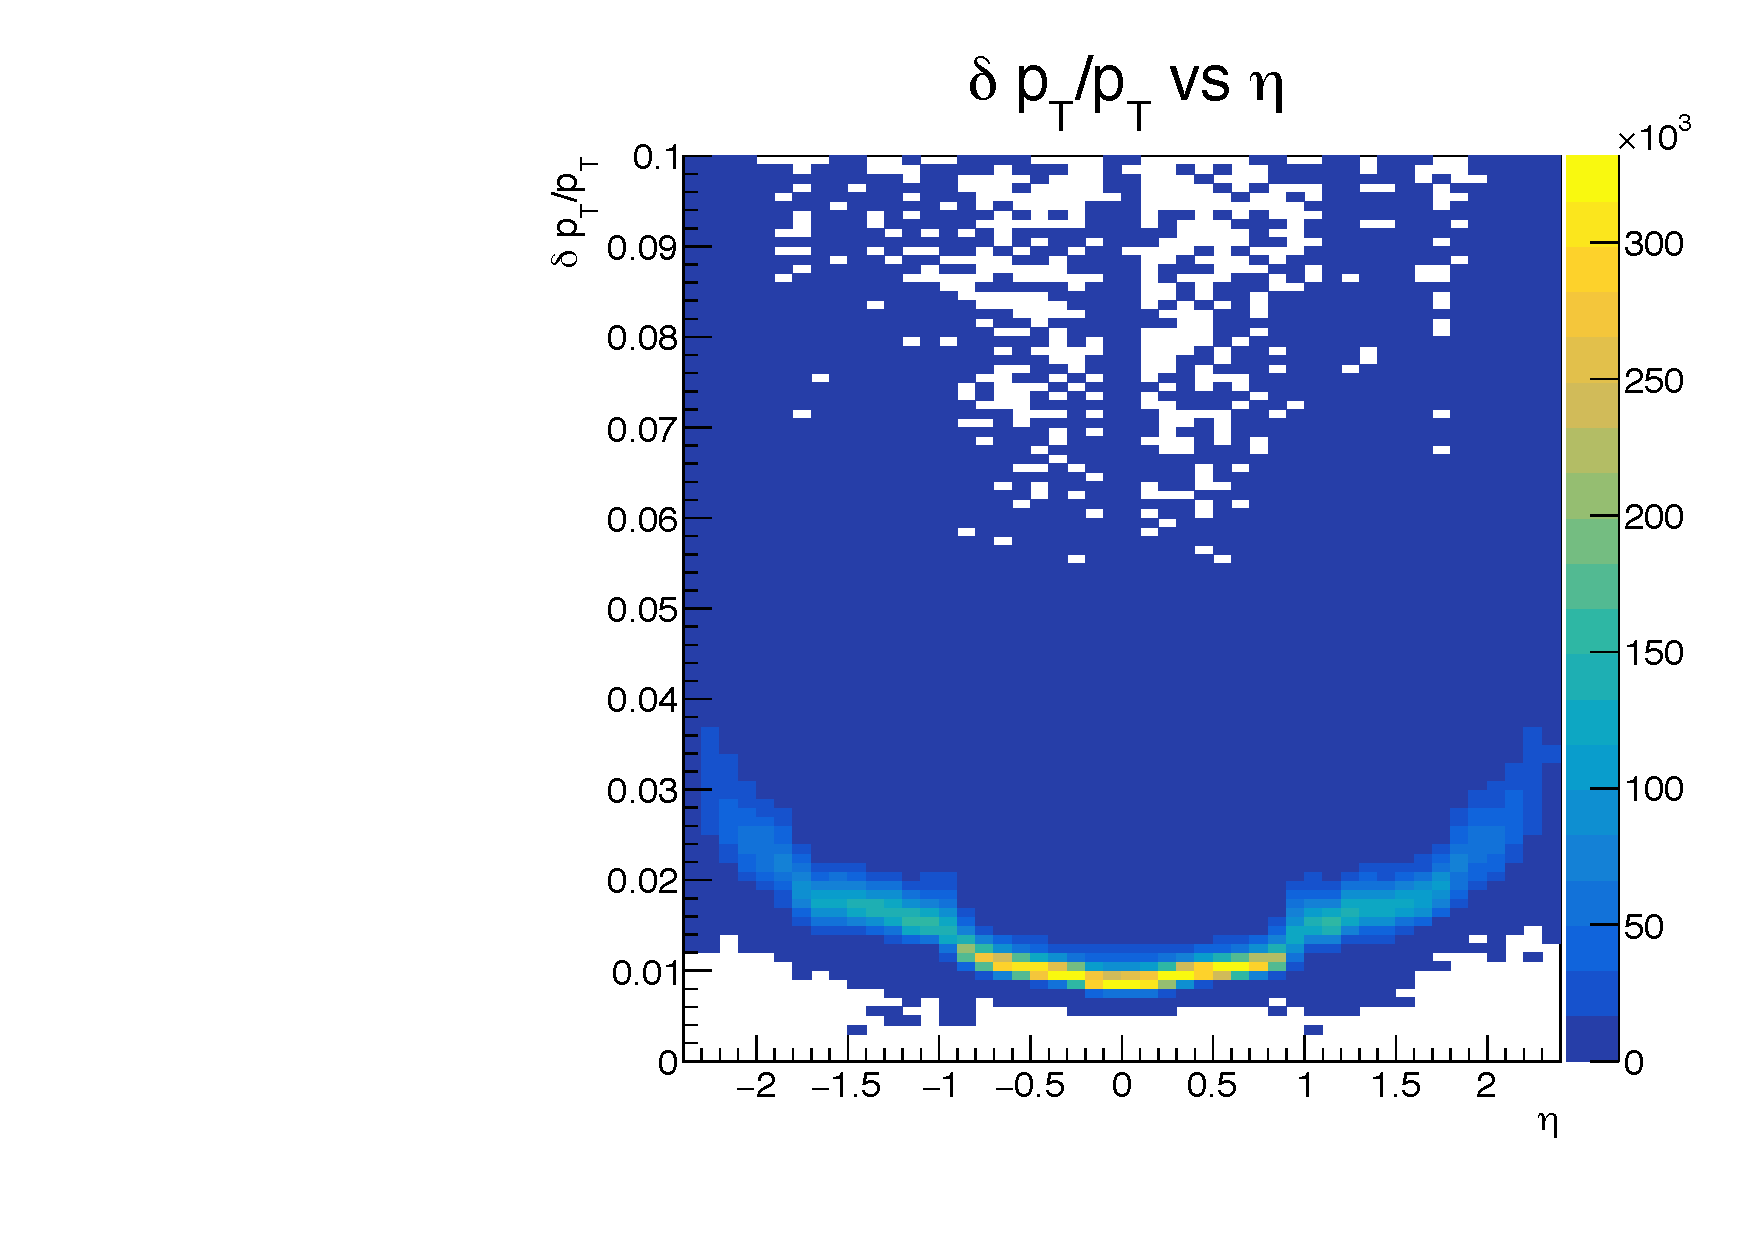
\includegraphics[width=0.32\textwidth]{Figures/EBE/2016_vs_eta_muon.pdf}
% 					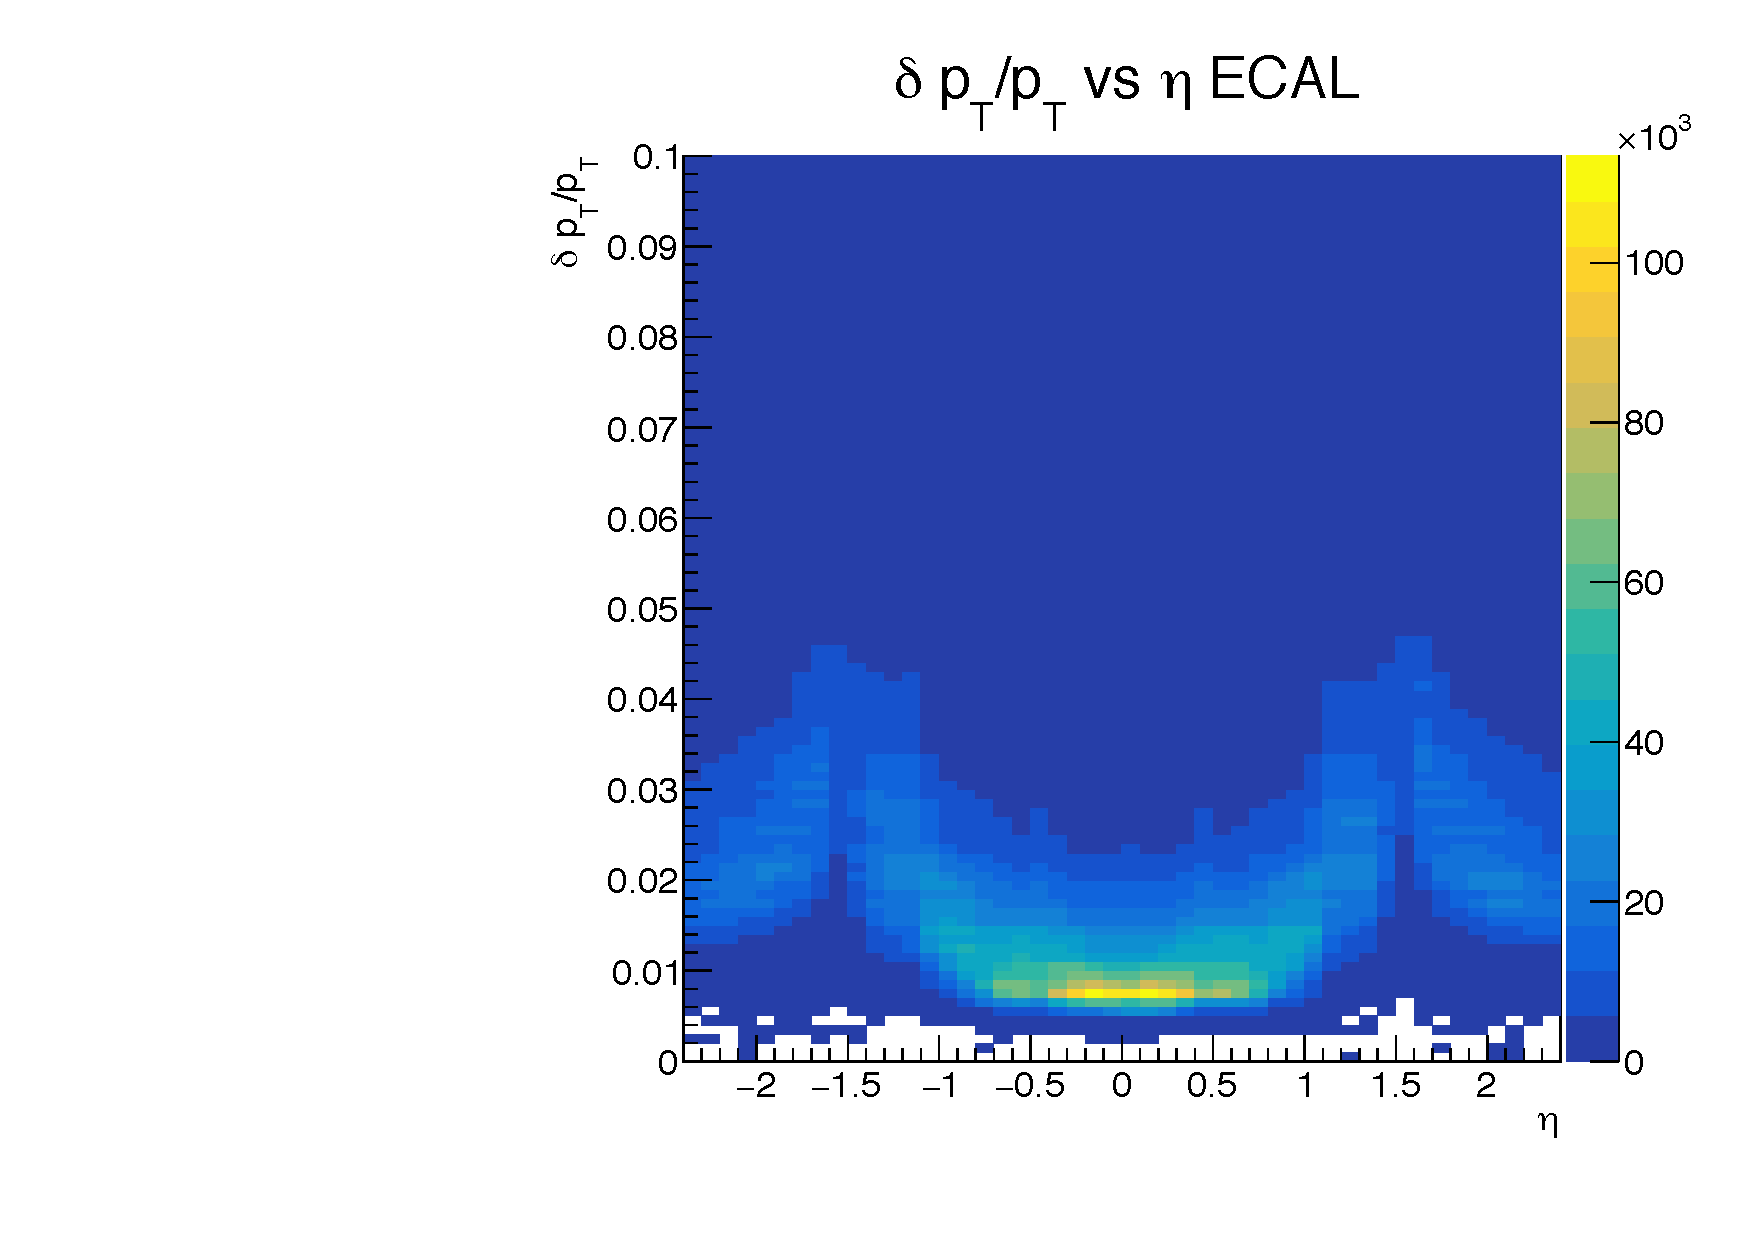
\includegraphics[width=0.32\textwidth]{Figures/EBE/2016_vs_eta_ele_ECAL.pdf} 
% 					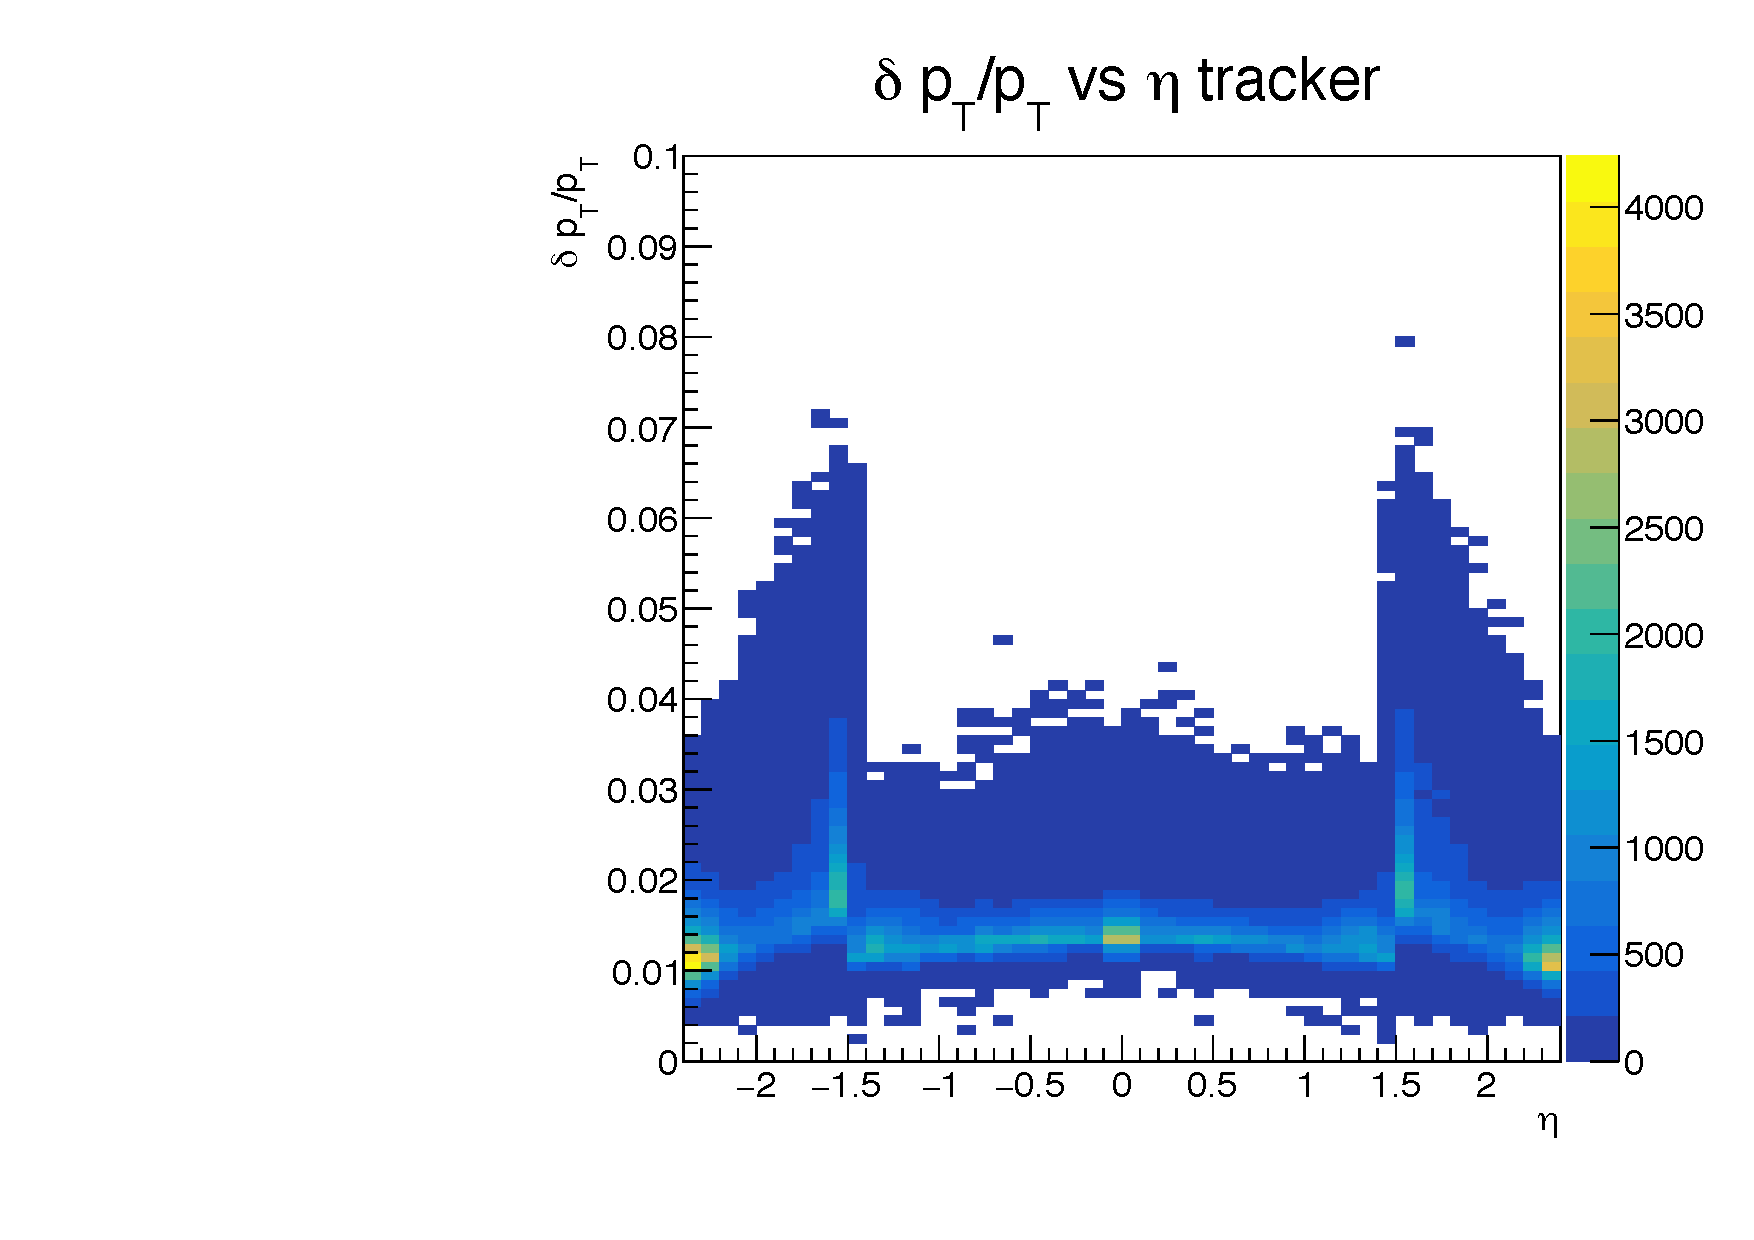
\includegraphics[width=0.32\textwidth]{Figures/EBE/2016_vs_eta_ele_tracker.pdf}
% %			}\\
% %		\subfloat[][2017]
%             % {
% 		    		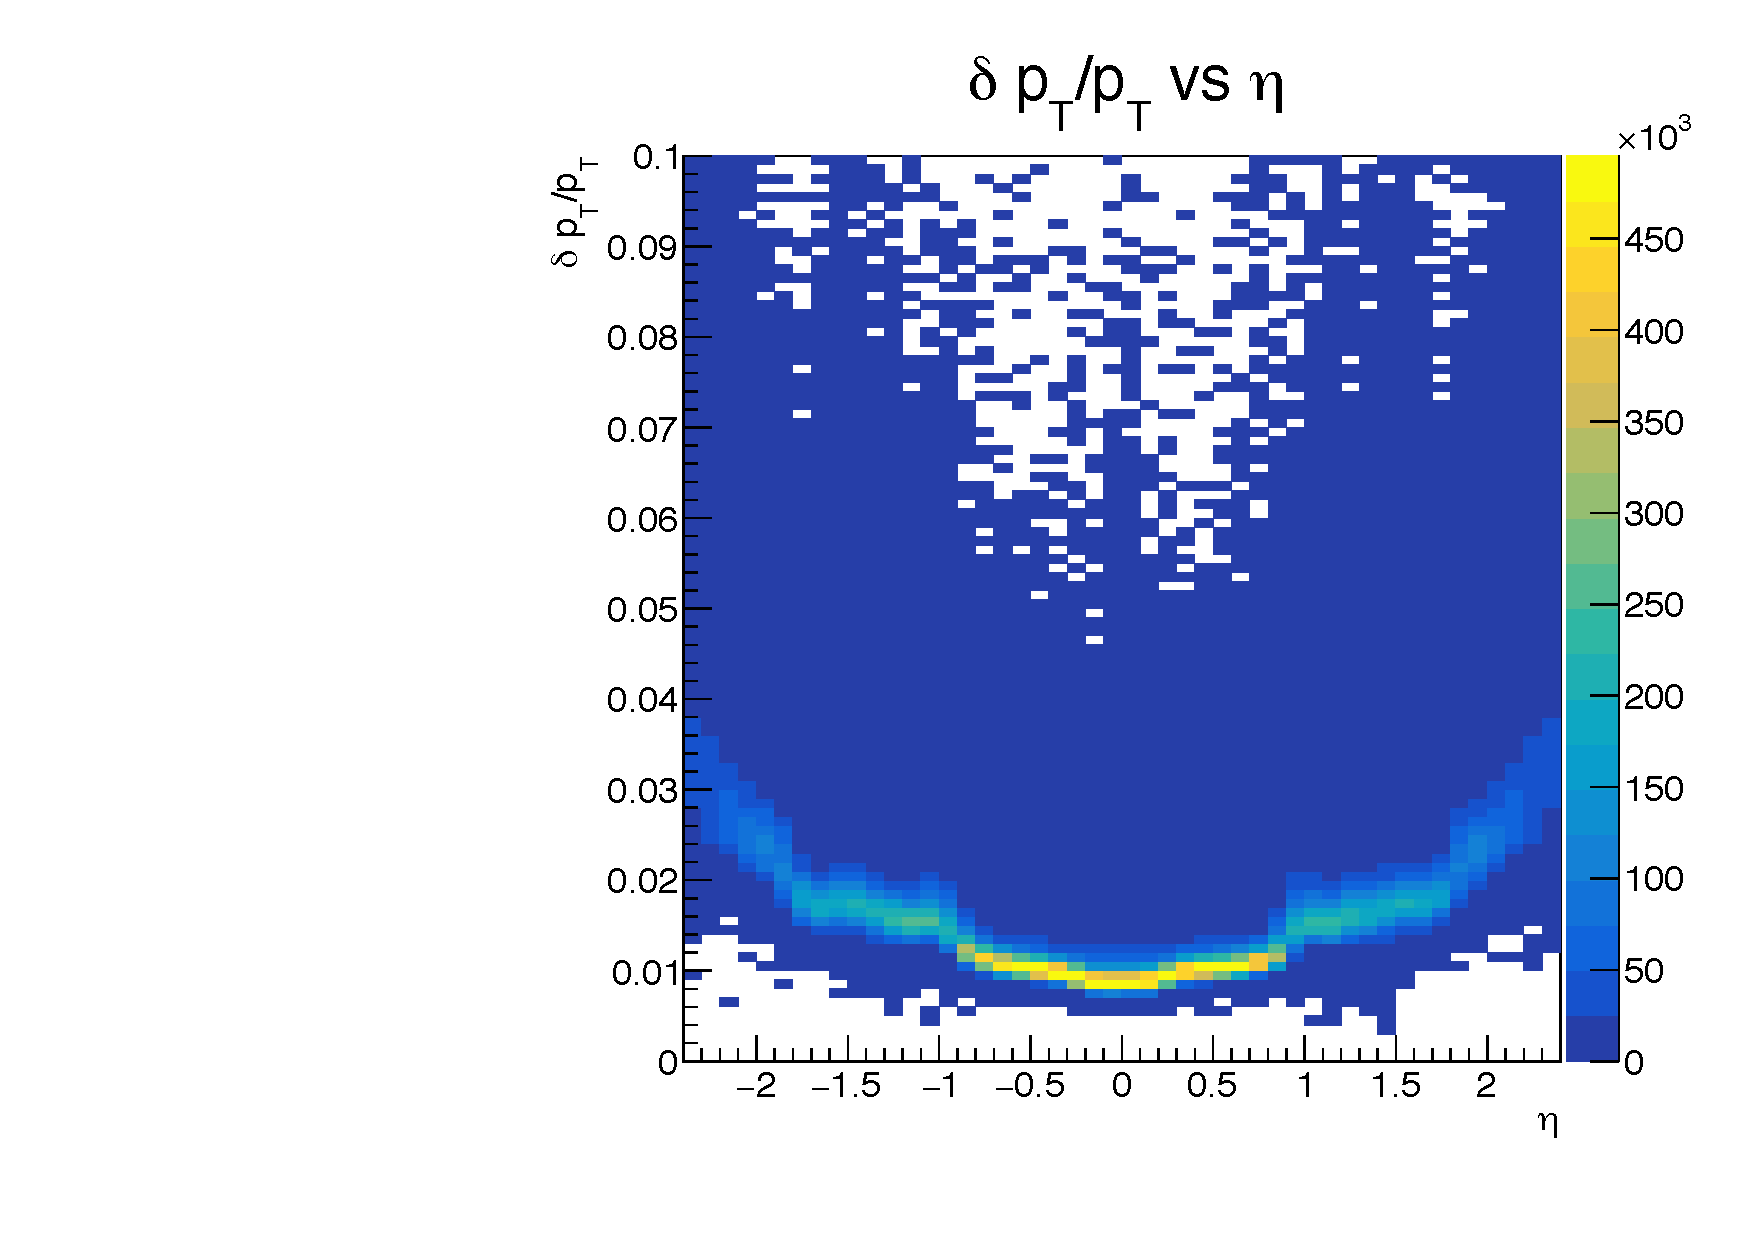
\includegraphics[width=0.32\textwidth]{Figures/EBE/2017_vs_eta_muon.pdf}
% 					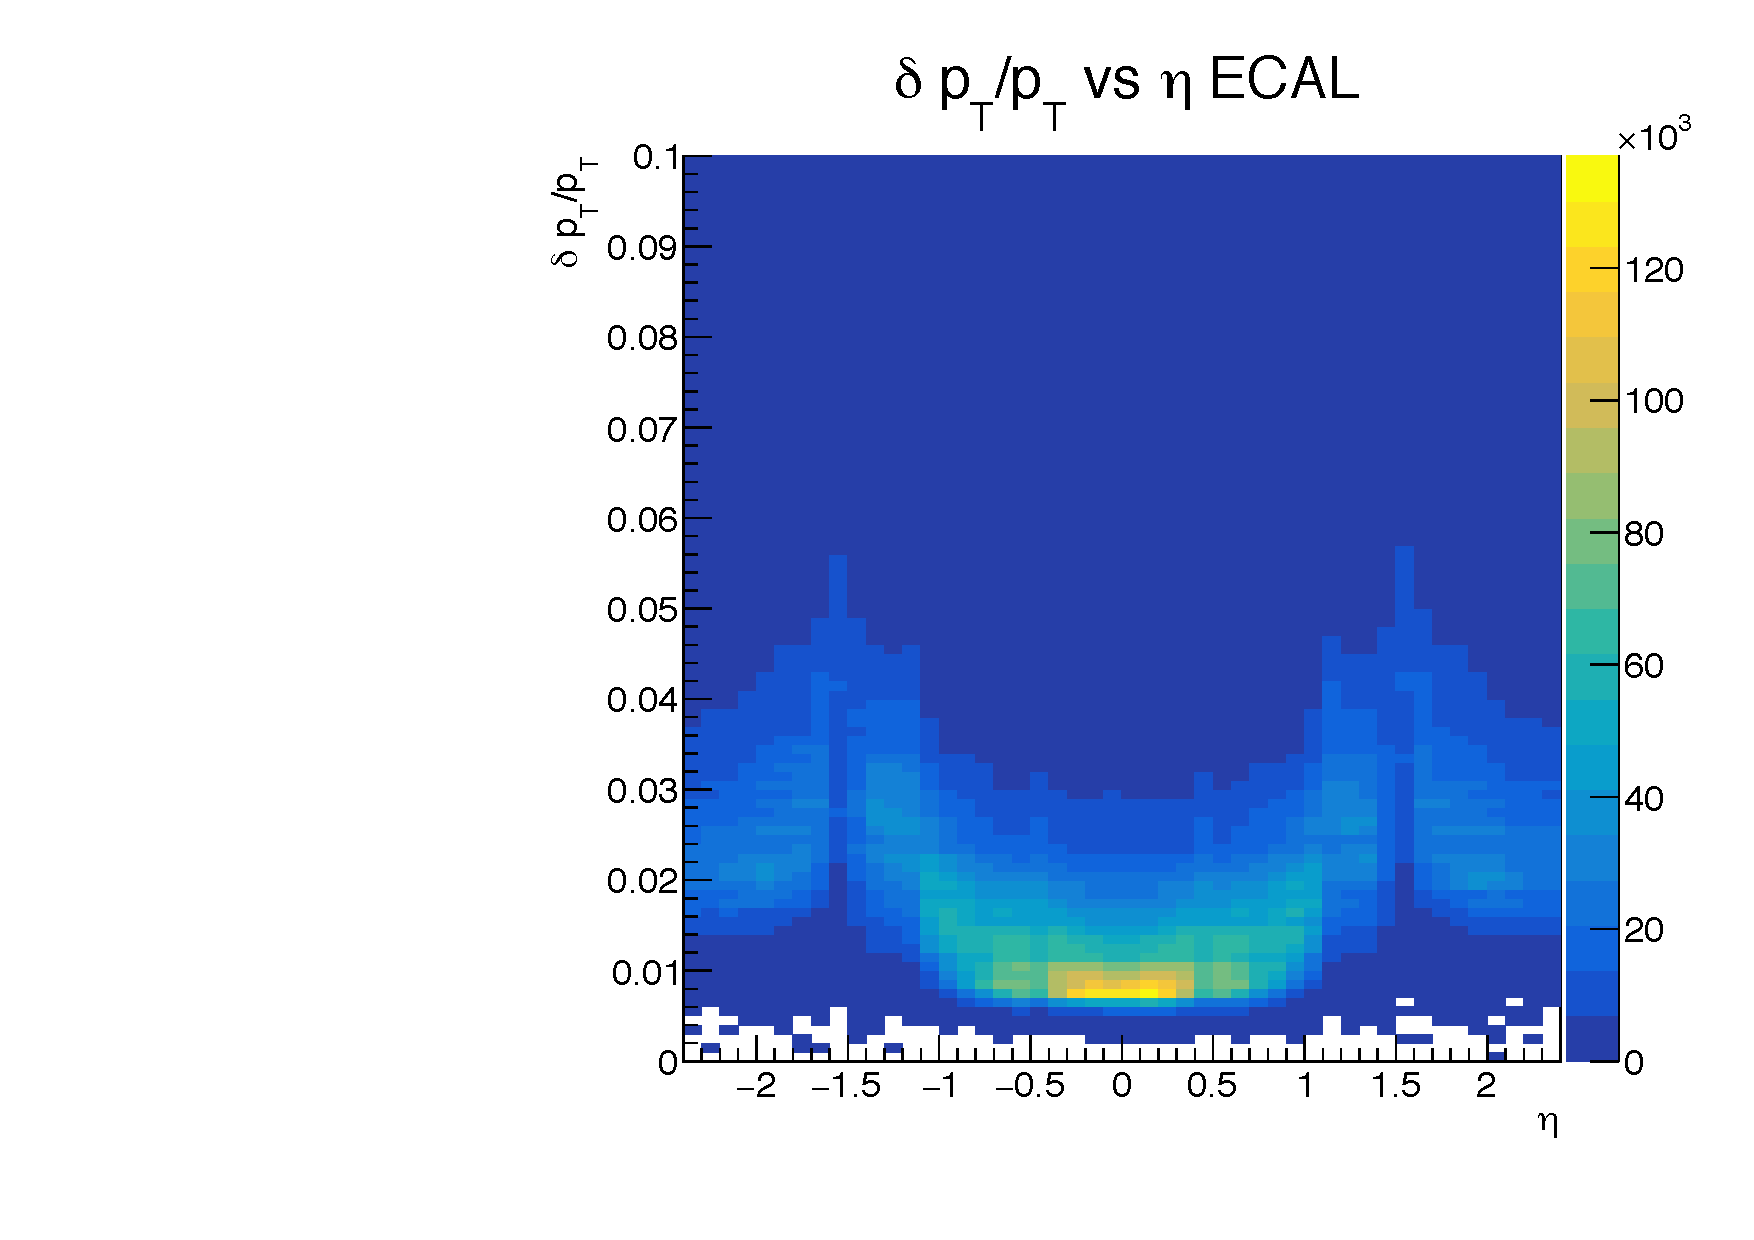
\includegraphics[width=0.32\textwidth]{Figures/EBE/2017_vs_eta_ele_ECAL.pdf} 
% 					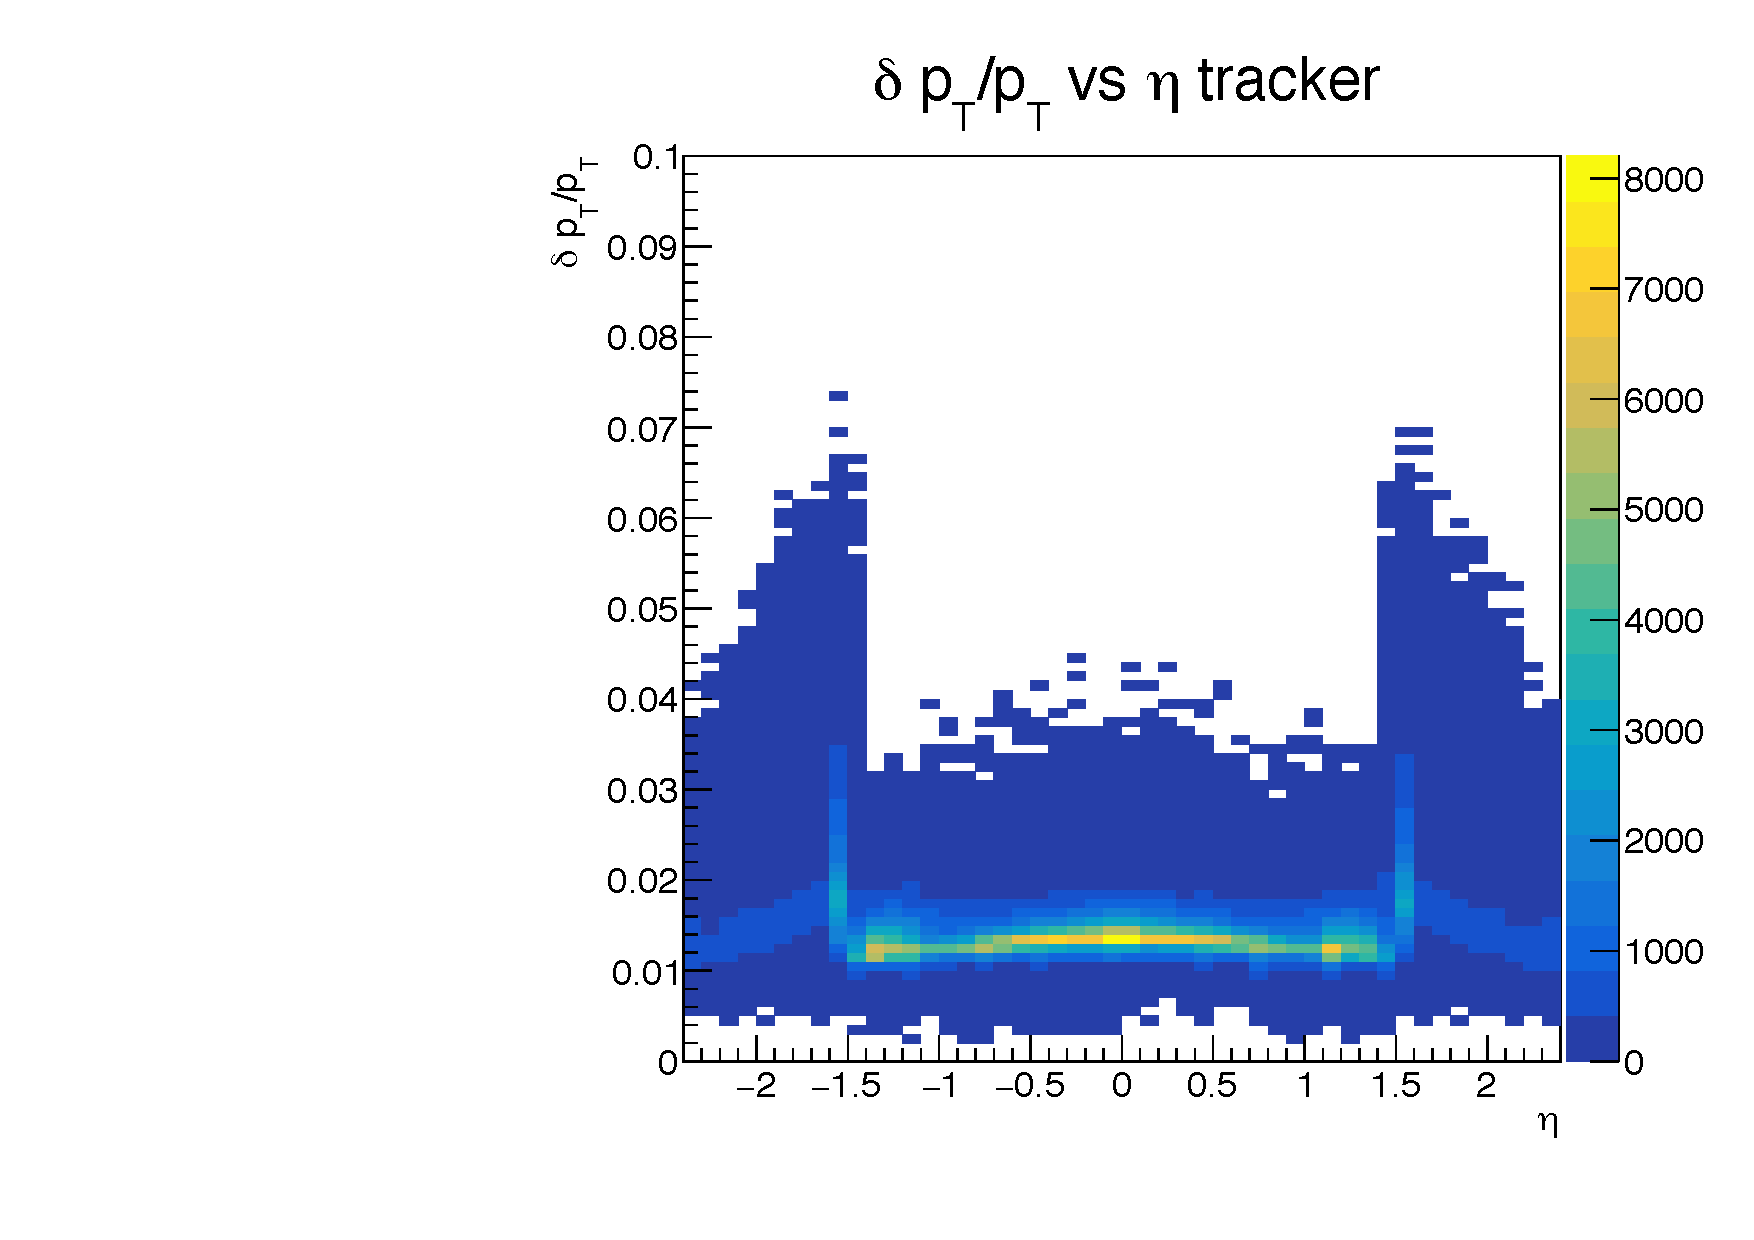
\includegraphics[width=0.32\textwidth]{Figures/EBE/2017_vs_eta_ele_tracker.pdf}
% %			}\\
% %		\subfloat[][2018]
%             % {
% 		    		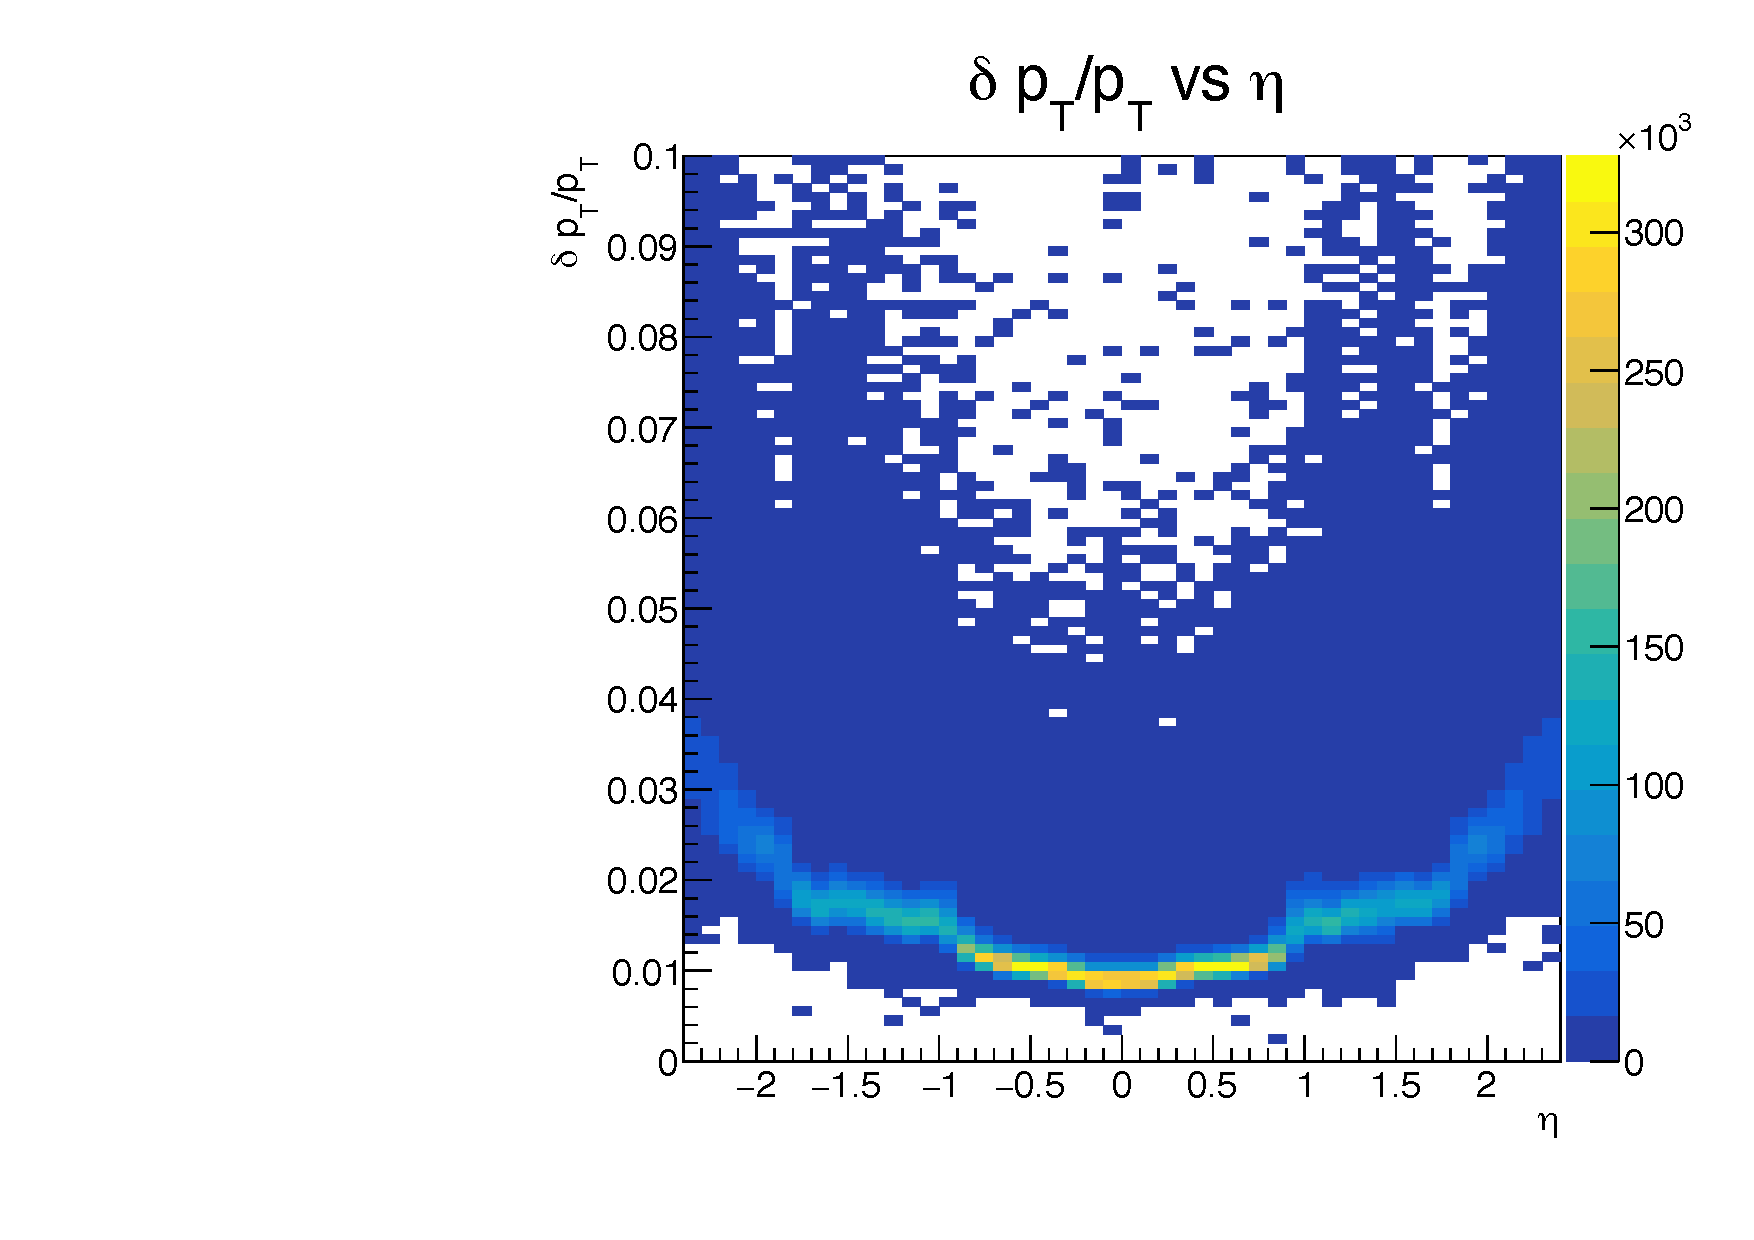
\includegraphics[width=0.32\textwidth]{figures/higgsmassmeas/ebe/2018_vs_eta_muon.pdf}
% 					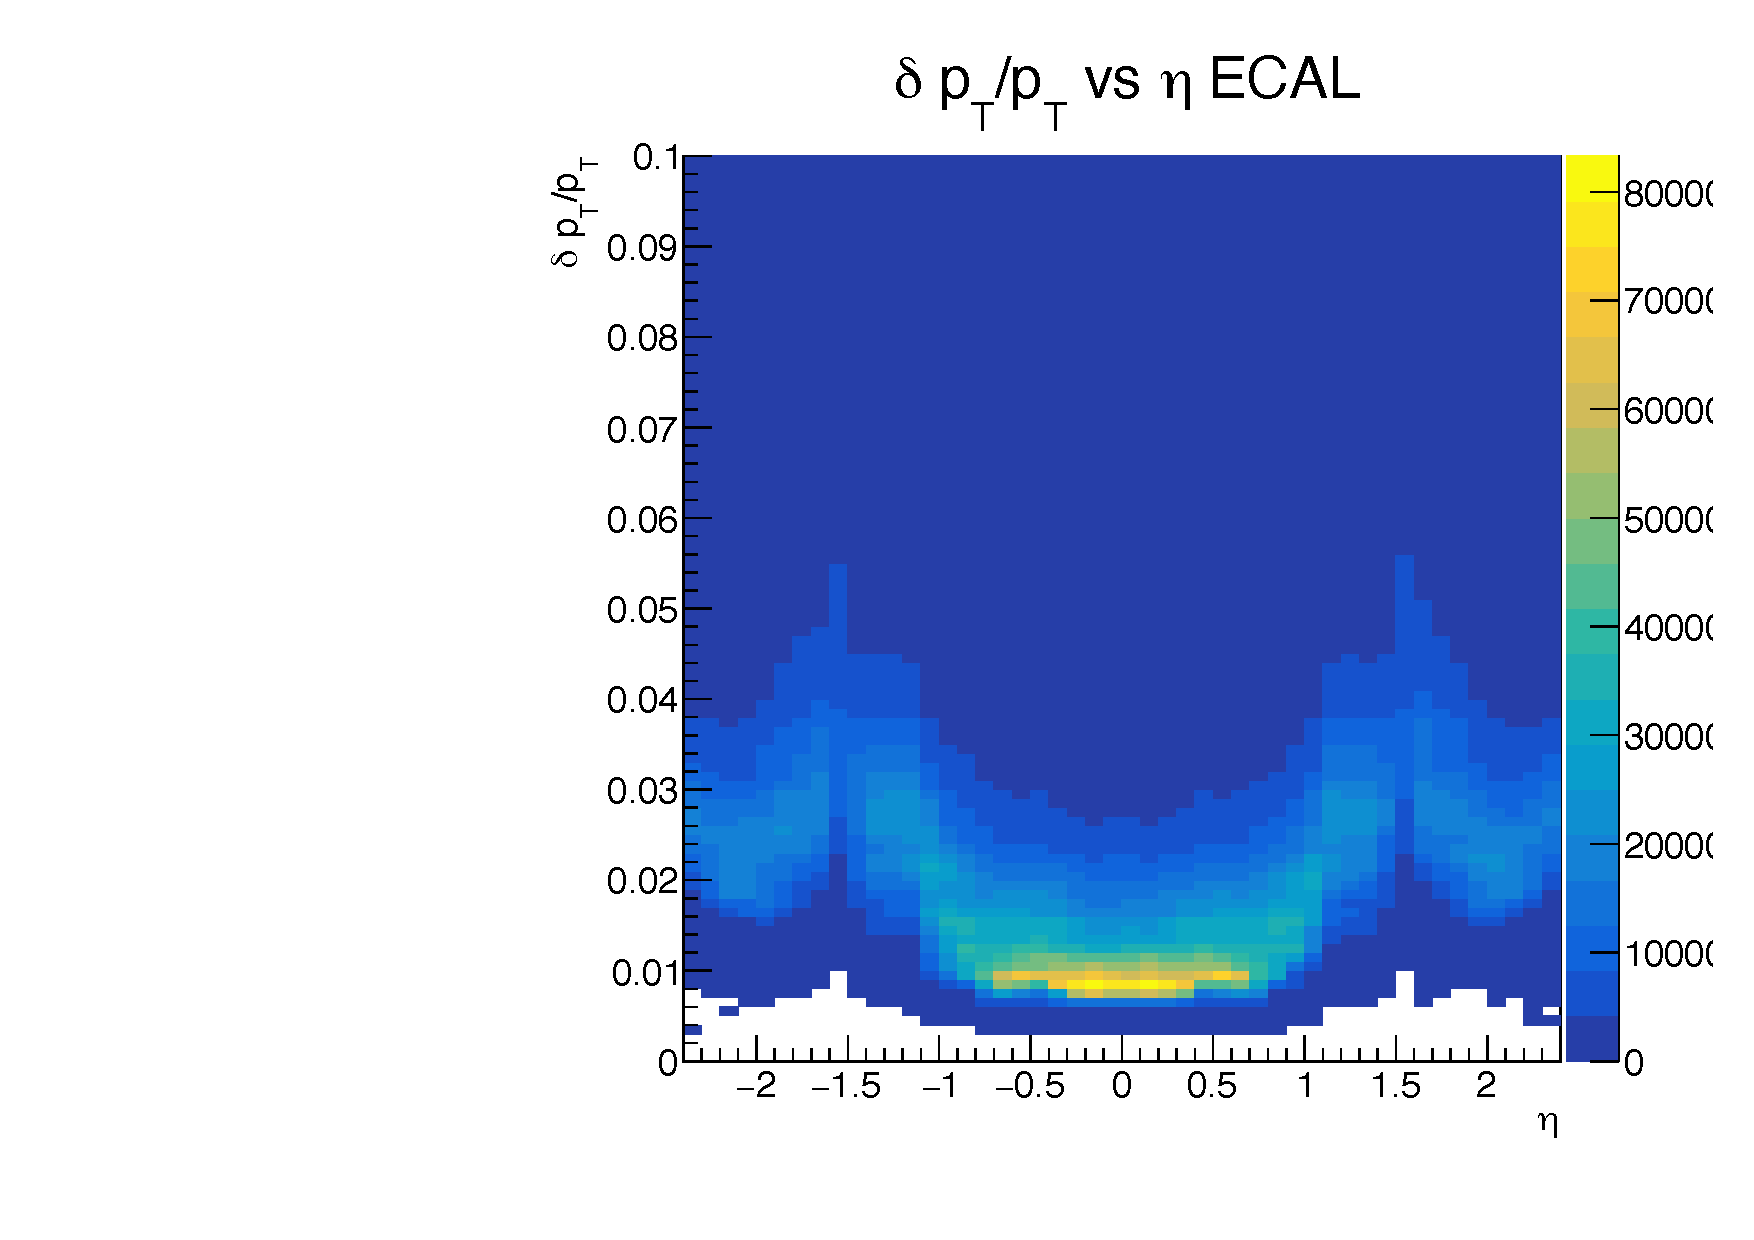
\includegraphics[width=0.32\textwidth]{figures/higgsmassmeas/ebe/2018_vs_eta_ele_ECAL.pdf} 
% 					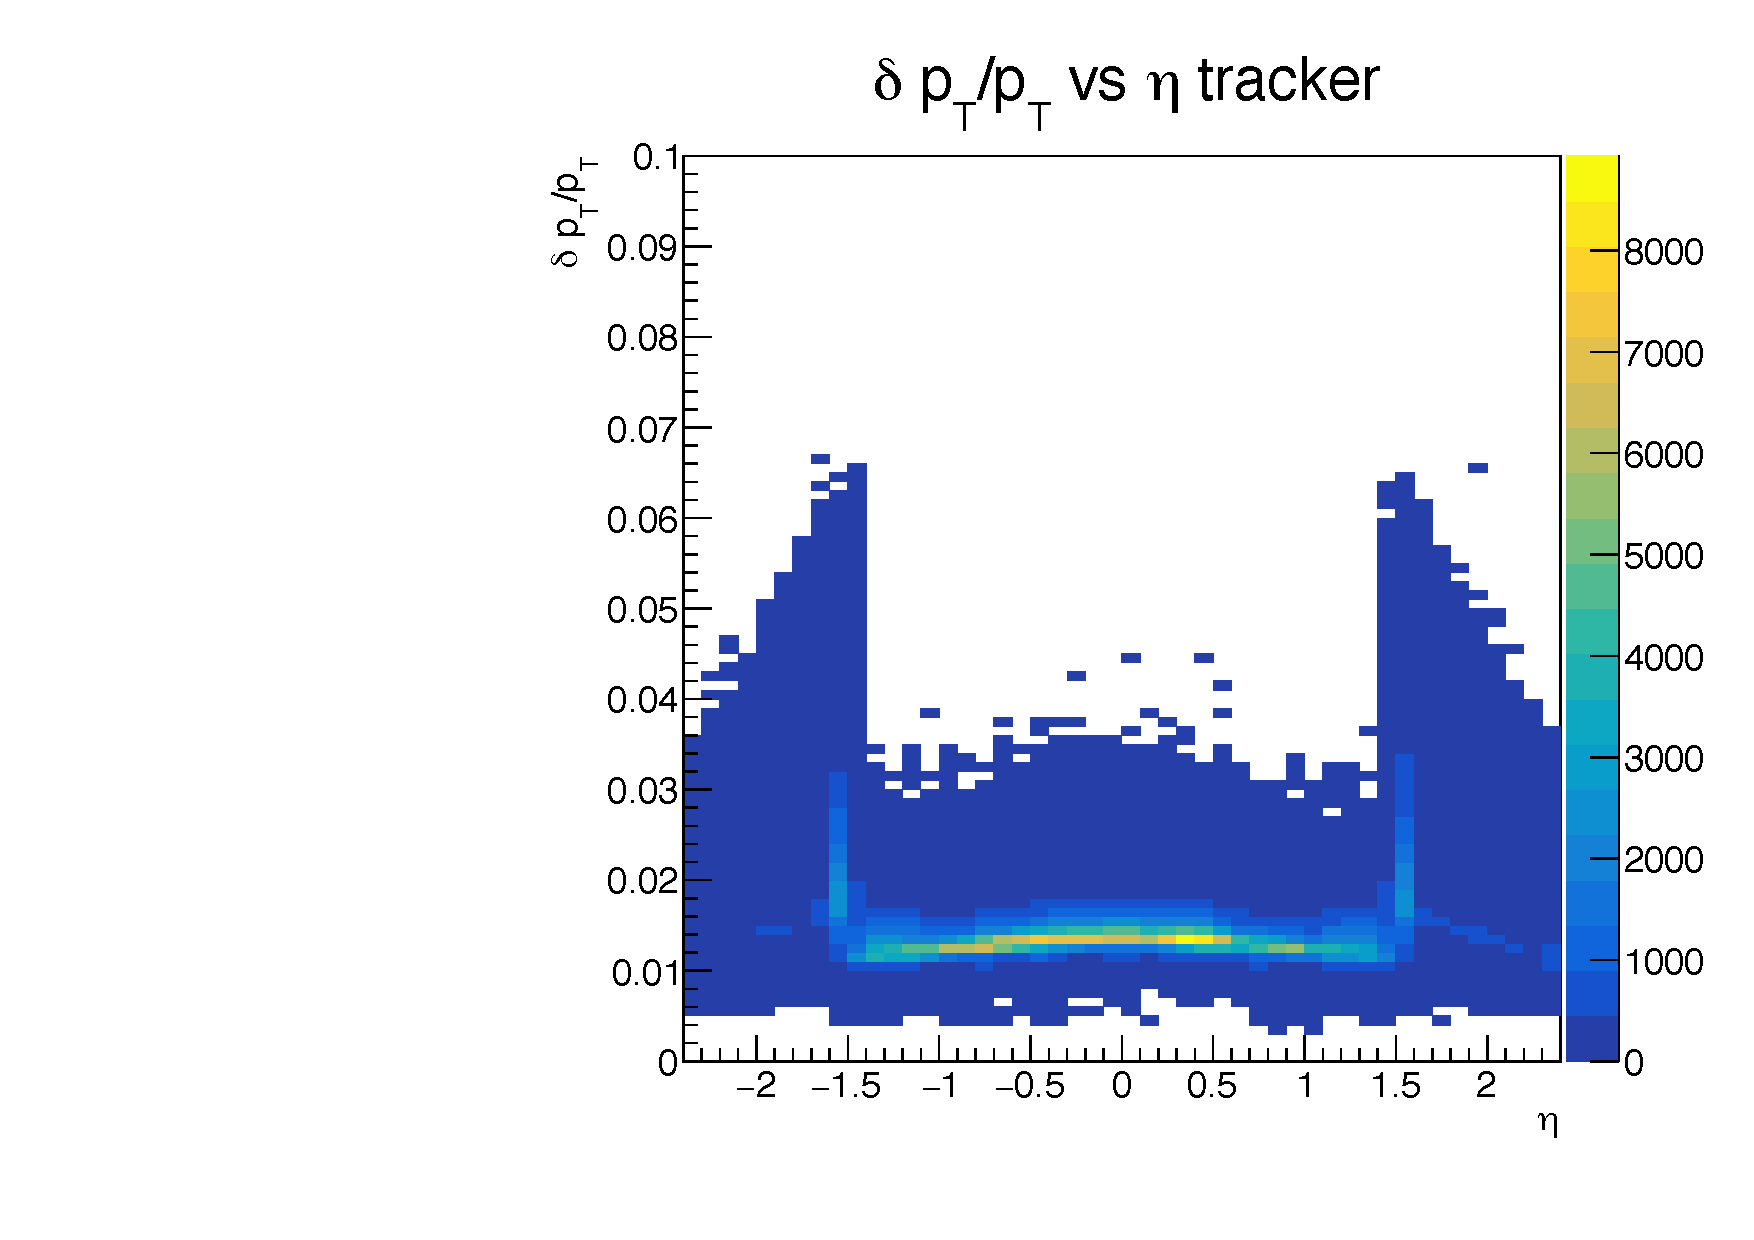
\includegraphics[width=0.32\textwidth]{figures/higgsmassmeas/ebe/2018_vs_eta_ele_tracker.pdf}
% %			}\\
% 		\caption{Scatter plot of the relative lepton \PT error vs $\eta$ for muons (left), 
% 				ECAL driven electrons (middle), and tracker driven electrons (right) for 2018 data.}
% 	\label{fig:2D_Mpas_vs_eta}
% 	\end{center}
% \end{figure}

TODO:REWORD, CONTAINS DATA
Starting from these distributions, corrections to momentum uncertainty in mutual $|\eta|$ bins are derived for muons (Fig.~\ref{fig:2D_Mpas_vs_pt_muon}), ECAL-driven electrons (Fig.~\ref{fig:2D_Mpas_vs_pt_electron_ECAL}), and tracker electrons (Fig.~\ref{fig:2D_Mpas_vs_pt_electron_tracker}) using bins of $\delta p_{T}$/$p_{T}$ \vs \abseta.
The scatter plots $\delta p_{T}$/$p_{T}$ \vs \PT are shown in Figs.~\ref{fig:2D_Mpas_vs_pt_electron_ECAL} and~\ref{fig:2D_Mpas_vs_pt_electron_tracker}.
% Muons.
\begin{multiFigure}
    \centering
    \addFigure{0.32}{figures/higgsmassmeas/ebe/2016_vs_pt_muon_1.pdf}
    \addFigure{0.32}{figures/higgsmassmeas/ebe/2016_vs_pt_muon_2.pdf}
    \addFigure{0.32}{figures/higgsmassmeas/ebe/2016_vs_pt_muon_3.pdf}

    \addFigure{0.32}{figures/higgsmassmeas/ebe/2017_vs_pt_muon_1.pdf}
    \addFigure{0.32}{figures/higgsmassmeas/ebe/2017_vs_pt_muon_2.pdf}
    \addFigure{0.32}{figures/higgsmassmeas/ebe/2017_vs_pt_muon_3.pdf}

    \addFigure{0.32}{figures/higgsmassmeas/ebe/2018_vs_pt_muon_1.pdf}
    \addFigure{0.32}{figures/higgsmassmeas/ebe/2018_vs_pt_muon_2.pdf}
    \addFigure{0.32}{figures/higgsmassmeas/ebe/2018_vs_pt_muon_3.pdf}
    \captionof{figure}
        [words.]
        {Scatter plot of the relative lepton \PT error vs \PT for muons with $0 < \abseta < 0.9$ (left column), $0.9 < \abseta < 1.8$ (middle column), and $1.8 < \abseta < 2.4$ (right column) for 2016 (top row), 2017 (middle row), and 2018 (bottom row) data.}
    \label{fig:2D_Mpas_vs_pt_muon}
\end{multiFigure}
% ECAL electrons.
\begin{multiFigure}
    \centering
    \addFigure{0.32}{figures/higgsmassmeas/ebe/2016_vs_pt_ECAL_1.pdf}
    \addFigure{0.32}{figures/higgsmassmeas/ebe/2016_vs_pt_ECAL_2.pdf}
    \addFigure{0.32}{figures/higgsmassmeas/ebe/2016_vs_pt_ECAL_3.pdf}

    \addFigure{0.32}{figures/higgsmassmeas/ebe/2017_vs_pt_ECAL_1.pdf}
    \addFigure{0.32}{figures/higgsmassmeas/ebe/2017_vs_pt_ECAL_2.pdf}
    \addFigure{0.32}{figures/higgsmassmeas/ebe/2017_vs_pt_ECAL_3.pdf}

    \addFigure{0.32}{figures/higgsmassmeas/ebe/2018_vs_pt_ECAL_1.pdf}
    \addFigure{0.32}{figures/higgsmassmeas/ebe/2018_vs_pt_ECAL_2.pdf}
    \addFigure{0.32}{figures/higgsmassmeas/ebe/2018_vs_pt_ECAL_3.pdf}
    \captionof{figure}
        [words.]
        % TODO: Is it OK to skip over 1.0--2.0?
        {Scatter plot of the relative lepton \PT error vs \PT for ECAL-driven electrons with $0 < \abseta < 0.8$ (left column), $0.8 < \abseta < 1.0$ (middle column), and $2.0 < \abseta < 2.5$ (right column) for 2016 (top row), 2017 (middle row), and 2018 (bottom row) data.}
    \label{fig:2D_Mpas_vs_pt_electron_ECAL}
\end{multiFigure}
% Tracker electrons.
\begin{multiFigure}
    \centering
    \addFigure{0.32}{figures/higgsmassmeas/ebe/2016_vs_pt_tracker_1.pdf}
    \addFigure{0.32}{figures/higgsmassmeas/ebe/2016_vs_pt_tracker_2.pdf}
    \addFigure{0.32}{figures/higgsmassmeas/ebe/2016_vs_pt_tracker_3.pdf}

    \addFigure{0.32}{figures/higgsmassmeas/ebe/2017_vs_pt_tracker_1.pdf}
    \addFigure{0.32}{figures/higgsmassmeas/ebe/2017_vs_pt_tracker_2.pdf}
    \addFigure{0.32}{figures/higgsmassmeas/ebe/2017_vs_pt_tracker_3.pdf}

    \addFigure{0.32}{figures/higgsmassmeas/ebe/2018_vs_pt_tracker_1.pdf}
    \addFigure{0.32}{figures/higgsmassmeas/ebe/2018_vs_pt_tracker_2.pdf}
    \addFigure{0.32}{figures/higgsmassmeas/ebe/2018_vs_pt_tracker_3.pdf}
    \captionof{figure}
        [words.]
        % TODO: Is it OK to skip over 1.44--1.6?
        {Scatter plot of the relative lepton \PT error vs \PT for tracker-driven electrons with $0 < \abseta < 0.8$ (left column), $1.0 < \abseta < 1.44$ (middle column), and $1.6 < \abseta < 2.0$ (right column) for 2016 (top row), 2017 (middle row), and 2018 (bottom row) data.}
    \label{fig:2D_Mpas_vs_pt_electron_tracker}
\end{multiFigure}

% TODO: REWORD
\subsection{Model and procedure to derive corrections}
To derive the corrections ($\lambda$), the dilepton mass $m_{\ell\ell}$ is fitted twice with a 
Breit-Wigner (BW) convoluted with a Crystal Ball (CB), plus exponential function (EXP). In this model, 
the BW represents true $m_{Z}$ shape, the CB simulates the detector effect, and the EXP 
describes the background. When deriving corrections, mean and sigma of Z's BW shape have been set to PDG
values ($mean_{Z}$ = 91.19 \GeV,  $\sigma_{Z}$ = 2.49\GeV~\cite{particle_data_group_review_2020}).
 The fit is done in the mass range [60, 120]\GeV, using only
$e^{+}e^{-}$ or $\mu^{+}\mu^{-}$ pairs.\\
The first fit is used to fix all the parameters of the functions but the $\sigma$ of the CB which is
replaced in the second fit by $\lambda$ $\times$ $\delta_{m_{Z}}$, where $\lambda$ is the 
floated parameter of the fit. 

%If statistics is large enough for a...\textbf{DECIDE HOW TO BEHAVE IN CASE OF LACK OF STATISTCS}.

The summary of $\lambda$ correction factors for electrons and muons is presented in \tablename~\ref{table:Lambdas}.
% TODO:Table below CONTAINS DATA. Make it work?
% \begin{table}[ht]	
% 	\begin{center}
% 		\begin{tabular}{ccccccc}
% 			\hline
% 			\hline			
% 			& \multicolumn{2}{c}{\textbf{2016}} & \multicolumn{2}{c}{\textbf{2017}} & \multicolumn{2}{c}{\textbf{2018}} \\
% 			& \multicolumn{1}{c}{\textbf{MC}} & \multicolumn{1}{c}{\textbf{Data}} & \multicolumn{1}{c}{\textbf{MC}} & \multicolumn{1}{c}{\textbf{Data}} & \multicolumn{1}{c}{\textbf{MC}} & \multicolumn{1}{c}{\textbf{Data}} \\
% 			\hline
% 			\hline
% 			& \multicolumn{6}{c}{Muons} \\
% 			$ 0 < |\eta| < 0.9$ &	1.05	&	1.248	&	1.043	&	1.214	&	1.047		&	1.183	&	1.019	&	1.227	\\
%                        $ 0.9 < |\eta| < 1.8$ &	1.187	&	1.256	&	1.204	&	1.234	&	1.219	&	1.223	&	1.206	&	1.236	\\
%                        $ 1.8 < |\eta| < 2.4$ &	1.197	&	1.201	&	1.183	&	1.164	&	1.197	&	1.173	&	1.108	&	1.188	\\
% 			\hline
% 			\hline
% 			& \multicolumn{6}{c}{ECAL electrons} \\
% 			$0 < |\eta| < 0.8$ and $\delta\pt/\pt < 0.01$            & 2.006 & 1.893 & 2.086 & 2.030 & 2.054 & 1.914 \\
%                        $0 < |\eta| < 0.8$ and $0.01 < \delta\pt/\pt < 0.015$    & 1.590 & 1.575 & 1.698 & 1.680 & 1.701 & 1.635\\
%                        $0 < |\eta| < 0.8$ and $0.015 < \delta\pt/\pt < 0.025$   & 1.406 & 1.373 & 1.426 & 1.450 & 1.447 & 1.467\\
%                        $0 < |\eta| < 1$ and $0.025 < \delta\pt/\pt < 1$         & 1.517 & 1.531 & 1.481 & 1.521 & 1.560 & 1.569\\
%                        $1 < |\eta| < 2.5$ and $\delta\pt/\pt < 0.02$            & 2.116 & 2.002 & 2.305 & 2.210 & 2.324 & 2.228\\
%                        $1 < |\eta| < 2.5$ and $0.02 < \delta\pt/\pt < 0.03$     & 1.645 & 1.623 & 1.815 & 1.795 & 1.787 & 1.759\\
%                        $1 < |\eta| < 2.5$ and $0.03 < \delta\pt/\pt < 0.04$     & 1.472 & 1.489 & 1.568 & 1.560 & 1.468 & 1.509\\
%                        $1 < |\eta| < 2.5$ and $0.04 < \delta\pt/\pt < 0.06$     & 1.374 & 1.448 & 1.414 & 1.606 & 1.378 & 1.477\\
%                        $0.8 < |\eta| < 1$ and $\delta\pt/\pt < 0.025$           & 1.149 & 1.203 & 1.196 & 1.241 & 1.180 & 1.286\\
%                        $1 < |\eta| < 2.5$ and $0.06 < \delta\pt/\pt < 1$        & 1.099 & 1.221 & 1.171 & 1.331 & 1.123 & 1.272\\
% 			\hline
% 			\hline
% 			& \multicolumn{6}{c}{tracker electrons} \\
% 			$0 < |\eta| < 1.44$ & 1.619 & 1.872 & 2.382 & 2.115 & 2.120 & 1.936\\
%                        $1.44 < |\eta| < 1.6$ & 6.452 & 5.900 & 6.572 & 7.056 & 5.613 & 5.524\\
%                        $1.6 < |\eta| < 2$ & 2.732 & 2.826 & 3.430 &2.846& 3.204 & 3.016\\
%                        $2 < |\eta| <2.5$ & 3.010 &3.081& 3.963 &3.817& 4.110 & 3.762\\
% 			\hline
% 		\end{tabular}
% 	\end{center}
% 	\caption{\PT error corrections for muons and electrons in different kinematic region. For each year, MC 
% 	is on the left, data on the right.}
% 	\label{table:Lambdas}
% \end{table}
% TODO: Figure 8 (from AN) of lambdas vs. dpT/pT bins? CONTAINS DATA.

% TODO: REWORD.
\subsubsection{Validation of corrections (MC, data)}
\label{sec:ClosureTest}
A closure test is performed to validate correction derived for lepton \PT error. \\
First, events are divided according to different predicted $\delta m_{Z}/m_{Z}$ ranges before corection. 
Then, in each bin, the dilepton mass distribution is fitted using a BW convoluted with CB 
plus exponential function, to get $\delta m_{Z}^{fit}$ (measured $m_{Z}$ resolution). Finally 
the average predicted $\delta m_{Z}$ is calculated in each $\delta m_{Z}/m_{Z}$ bin before and after the 
correction factor for lepton \PT error is applied (predicted $m_{Z}$ resolution). \\
In the closure plot, it is expected to see $\delta m_{Z}$ gets closer to $\delta m_{Z}^{fit}$ 
after correction, and the points should stay in a band which is 20\% around diagonal line, which 
is the uncertainty assigned to the resolution in the previous analysis \cite{HIG_16_041}. 
This closure test is shown in Fig.~\ref{fig:ZClosure_test_MU} for muons and in Fig.~\ref{ZClosure_test_ELE} 
for electrons. A further check has been also performed, looking at the closure test of the predicted four lepton mass 
resolution compared to the fitted four lepton mass resolution using ggF signal MC samples once the 
corrections derived using Z events are applied. After applying correction, measured $m_{4l}$ 
resolution gets closer to the prediction. This closure test is shown for three different 
final states in Fig.%~\ref{HClosure_test}.
% CLOSURE: Z->mumu MC.
\begin{multiFigure}
    \centering
    \addFigure{0.35}{figures/higgsmassmeas/ebe/VXBS_20160_MC.pdf}
    \addFigure{0.35}{figures/higgsmassmeas/ebe/VXBS_20165_MC.pdf}
    \addFigure{0.35}{figures/higgsmassmeas/ebe/VXBS_2017_MC.pdf}
    \addFigure{0.35}{figures/higgsmassmeas/ebe/VXBS_2018_MC.pdf}
    \captionof{figure}
        [TODO]
        {Validation of the per-event mass uncertainties from Z events in MC in the dimuon channel using 2016 pre-VFP (top left), 2016 post-VFP (top right), 2017 (bottom left), and 2018 (bottom right) events.
		The solid blue line corresponds to a 10\% band relative to the solid green 1:1 line.}
    \label{fig:ZClosure_test_MU}
\end{multiFigure}
% \begin{figure}[!htbp]
% 	\begin{center}
% 		\subfloat[][MC]
% 		   {		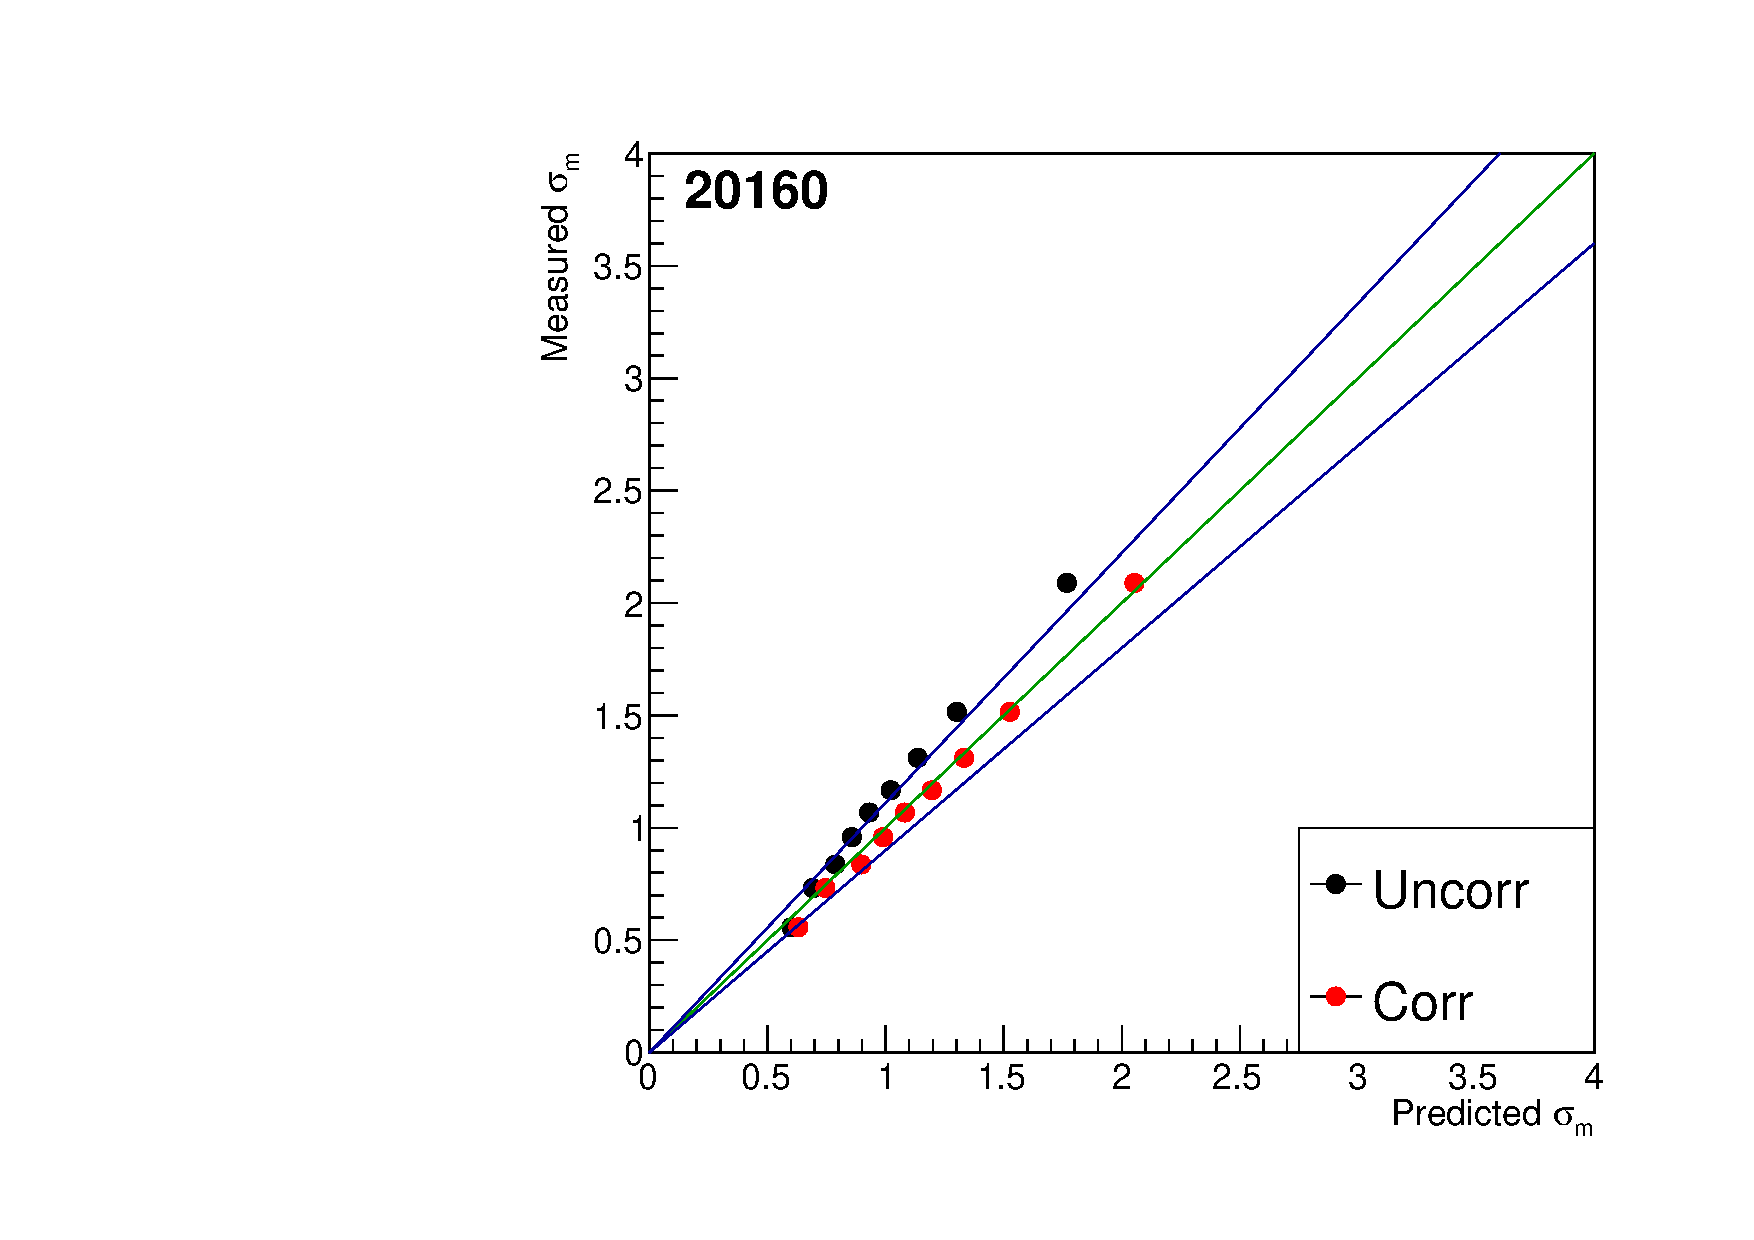
\includegraphics[width=0.35\textwidth]{Figures/EBE/VXBS_20160_MC.pdf}
% 					\includegraphics[width=0.35\textwidth]{Figures/EBE/VXBS_20165_MC.pdf}
% 					\includegraphics[width=0.35\textwidth]{Figures/EBE/VXBS_2017_MC.pdf}
% 					\includegraphics[width=0.35\textwidth]{Figures/EBE/VXBS_2018_MC.pdf}
% 			}\\
% 		\subfloat[][Data]
% 		   {		\includegraphics[width=0.35\textwidth]{Figures/EBE/VXBS_20160_DATA.pdf}
% 					\includegraphics[width=0.35\textwidth]{Figures/EBE/VXBS_20165_DATA.pdf}
% 					\includegraphics[width=0.35\textwidth]{Figures/EBE/VXBS_2017_DATA.pdf}
% 					\includegraphics[width=0.35\textwidth]{Figures/EBE/VXBS_2018_DATA.pdf}
% 			}\\
% 		\caption{Validation of the per-event mass uncertainties from Z events in MC (top) and Data (bottom) 
% 		in dimuon channel in 2016 (top - pre and post VFP), 2017 (bottom left) and 2018 (bottom right). 
% 		10\% reference band is also shown.}
% 		\label{ZClosure_test_MU}
% 	\end{center}
% \end{figure}
% CLOSURE: Z->ee MC.
\begin{multiFigure}
    \centering
    \addFigure{0.35}{figures/higgsmassmeas/ebe/ZEE_20160_MC.pdf}
    \addFigure{0.35}{figures/higgsmassmeas/ebe/ZEE_20165_MC.pdf}
    \addFigure{0.35}{figures/higgsmassmeas/ebe/ZEE_2017_MC.pdf}
    \addFigure{0.35}{figures/higgsmassmeas/ebe/ZEE_2018_MC.pdf}
    \captionof{figure}
        [TODO]
        {Validation of the per-event mass uncertainties from Z events in MC in the dielectron channel using 2016 pre-VFP (top left), 2016 post-VFP (top right), 2017 (bottom left), and 2018 (bottom right) events.
		The solid blue line corresponds to a 10\% band relative to the solid green 1:1 line.}
    \label{fig:ZClosure_test_ELE}
\end{multiFigure}
% CLOSURE: ggH4l MC.
\begin{multiFigure}
    \centering
    \addFigure{0.32}{figures/higgsmassmeas/ebe/2016_H4mu_Closure_test.png}
    \addFigure{0.32}{figures/higgsmassmeas/ebe/2017_H4mu_Closure_test.png}
    \addFigure{0.32}{figures/higgsmassmeas/ebe/2018_H4mu_Closure_test.png}

    \addFigure{0.32}{figures/higgsmassmeas/ebe/2016_H4e_Closure_test.png}
    \addFigure{0.32}{figures/higgsmassmeas/ebe/2017_H4e_Closure_test.png}
    \addFigure{0.32}{figures/higgsmassmeas/ebe/2018_H4e_Closure_test.png}

    \addFigure{0.32}{figures/higgsmassmeas/ebe/2016_H2e2mu_Closure_test.png}
    \addFigure{0.32}{figures/higgsmassmeas/ebe/2017_H2e2mu_Closure_test.png}
    \addFigure{0.32}{figures/higgsmassmeas/ebe/2018_H2e2mu_Closure_test.png}
    \captionof{figure}
        [TODO]
        {Validation of the per-event mass uncertainties from events in \gghtofourl channel, in MC, 
		for three different final states (4\Pmu on top, 4e in the middle and 2e2\Pmu on bottom), 
		for three years (2016 on the left, 2017 in the middle, 2018 on the right).
		The 20\% reference band is also shown.}
    \label{fig:HClosure_test}
\end{multiFigure}


% \section{Background Estimation}
\label{sec:bkg_estim}
Measurement of the Higgs boson mass requires the accurate modeling of the total event yield in the signal region (SR), into which events can be categorized as either \emph{signal} or \emph{background}.
These background events pass the signal event selection (Section~\ref{sec:zz_sel}) and thus spoil the purity of the signal events.
This introduces further uncertainty into the final Higgs boson mass measurement.
Therefore, it is a priority to reduce and to predict the expected number of background events, which can be split into two types: \emph{irreducible background} (IB) and \emph{reducible background} (RB) processes.

\subsection{Irreducible Background}
\label{sec:bkg_irred}
IB processes produce two \PZ bosons and each \PZ subsequently decays into two prompt leptons (leptons that emerge directly from the primary vertex).
This reliably produces a \fourl final state, whose prompt leptons are typically reconstructed as four leptons that pass tight selection (\emph{PTS leptons}), as defined in Sections~\ref{sec:el_sel} and~\ref{sec:mu_sel}.
The IB event then looks indistinguishable from the 4 PTS lepton of the \emph{signal} process and cannot be reduced;
Thus, throwing away IB process could mean throwing away a signal event.
Since IB events cannot be completely eliminated---or \emph{reduced}---from the SR, they are given the name \emph{irreducible} backgrounds.
The two IBs for this analysis are:
\begin{itemize}
    \item \ggzzfourl (gluon-gluon fusion),
    \item \qqzzfourl (quark-antiquark annihilation).
\end{itemize}

\subsection{Reducible Background}
\label{sec:redbkg}
While IB processes produce 4 prompt leptons, RB processes produce varying numbers of prompt and nonprompt leptons.
Nonprompt leptons emerge from 3 main sources:
\begin{itemize}
    \item misidentifying light-flavor hadrons (\eg, $\pi^{\pm}$) as leptons,
    \item heavy-flavor hadrons that decay mid-flight into leptons,
    \item and the asymmetric conversion of photons into electrons.
\end{itemize}

This analysis is tailored to efficiently reconstruct prompt(nonprompt) leptons as PTS(FTS) leptons.
Ideally, the SR would contain only the events with 4 prompt leptons, which would always be tagged as 4 PTS leptons.
However, sometimes a truly nonprompt lepton is misidentified as a PTS lepton (sometimes called a \emph{fake lepton}), depending on the kinematic properties of the lepton.
This misidentification rate ($f$, sometimes called the \emph{fake rate}) is due to imperfect detector performance, inefficiencies in reconstruction, and the specific choice of lepton selections used in the analysis.

If an event produces prompt and nonprompt leptons but is reconstructed as 4 PTS leptons (a 4P event), then it contaminates the SR.
These processes constitute the RB processes (sometimes called ``\ZplusX'').
Examples of RB processes for this analysis include:
\begin{itemize}
	\item \Zplusjets (yields 2 prompt leptons)
	\item \ttbarplusjets (yields 2 prompt leptons)
	\item \WZplusjets (yields 3 prompt leptons)
	\item $\ZZ/Zgammastar + \text{jets}$ (yields 4 prompt leptons).
\end{itemize}
The careful estimation of these RB contributions to the 4P region is necessary for the precise measurement of the Higgs boson mass.

\subsubsection{OS Method}
% \label{sec:os_method}
The goal of the OS Method is to estimate the number of opposite-sign same-flavor (OSSF) \fourl events produced by RB process that ``contaminate'' the 4P region $\left( \nfourPRB \right)$, given by Eq.~\ref{eqn:rbe_formula_final}.
% Since the $4\ell$ final state of the signal process consists of 2 pairs of OSSF leptons, the method is called the \emph{OS Method}.
However, the typical approach of using simulated samples does not model RB well, since RB processes (\eg, \Zplusjets) rely on higher-order effects like jet modelling which are not yet accurately simulated.
Instead, a data-driven approach is used.

The logic of the OS Method is to study events in data that are similar to, but not exactly the same as, those found in the 4P region.
Thus, events in data are sorted into 2 control regions (CRs), both of which are orthogonal to the 4P region and to each other:
\begin{itemize}
	\item the \emph{3P1F} CR (built from 3 PTS and 1 FTS leptons)
	\item the \emph{2P2F} CR (built from 2 PTS and 2 FTS leptons).
\end{itemize}
The event selection for the 2P2F and 3P1F CRs is almost identical to that of the SR (Section~\ref{sec:zz_sel}),
except that the FTS lepton(s) are required to build the \Ztwo.
The events that contribute mostly to the 2P2F(3P1F) CR are those that produce 2(3) prompt and 2(1) nonprompt leptons and are called \emph{2pr}(\emph{3pr}) events.
Similarly, the events that contribute mostly to the 4P SR are those that produce 4 prompt leptons and are called \emph{4pr} events.

The final formula for \nfourPRB is obtained by first supposing that event $k$ is a 2pr event and contributes to the 2P2F CR an event weight of $\wgttwoprompttotwoPtwoF^k$.
This weight is built from $\hat{w}^k$, which is the product of analysis weights (pileup, L1 pre-firing, \etc), and the reconstruction efficiencies ($\epsilon$) of each lepton ($\ell_n$):
\begin{equation}
	\label{eqn:wt_2prto2p2f}
	\wgttwoprompttotwoPtwoF^k = \hat{w}^k \cdot \effprpass(\ell_1^k) \cdot \effprpass(\ell_2^k) \cdot \effnpfail(\ell_3^k) \cdot \effnpfail(\ell_4^k),
\end{equation}
where the superscript of $\epsilon$ indicates the lepton promptness (pr = prompt, np = nonprompt),
the subscript indicates the lepton tightness status (P = PTS, F = FTS).
To simplify the equations that follow, $\hat{w}^k$ is set to unity.
%  \effprpass(\ell_1^k) is the efficiency of reconstructing $\ell_1$ from event $k$ as a \mathbf{P}TS lepton
% and \effnpfail(\ell_3^k) is the efficiency of reconstructing $\ell_3$ from event $k$ as a \mathbf{F}TS lepton
% where $\epsilon^{\mathrm{pr|np}}_{\mathrm{P|F}}$ is the efficiency of reconstructing a prompt/nonprompt lepton passing/failing tight selections.
If the reconstruction efficiencies of a particular category are the same for all $j$ leptons across all $k$ events $\left( \eg, ~ \effprpass(\ell_j^k) \equiv \effprpass \right)$, then Eq.~\ref{eqn:wt_2prto2p2f} reduces to:
\begin{equation}
	\label{eqn:wt_2prto2p2f_simp}
	\wgttwoprompttotwoPtwoF^k = 
	\left( \effprpass \right)^2 
	\left( \effnpfail \right)^2.
\end{equation}

Although a 2pr event mostly contributes to the 2P2F CR, a nonprompt lepton may be misidentified as a PTS lepton, depending on \effnppass.
Such an event would then fall into the 3P1F CR and, allowing for only one nonprompt PTS lepton at a time, contributes an effective weight of
\begin{align}
	\label{eqn:wt_2prto3p1f}
	\wgttwoprompttothreePoneF^k
	&= \left( \effprpass \right)^2 
	\left[
		\effnppass(\ell_1^k) \cdot \effnpfail(\ell_2^k) + \effnpfail(\ell_1^k) \cdot \effnppass(\ell_2^k)
	\right]
	\notag
	\\
	&= \left( \effprpass \right)^2
	\left[
		2 \effnppass \effnpfail
	\right].
\end{align}
Using the fact that a (non)prompt lepton is exclusively either PTS or FTS
$\left( \epsilon^\text{pr(np)}_\text{P} + \epsilon^\text{pr(np)}_\text{F} = 1 \right)$,
% \begin{equation*}
% 	\epsilon^\mathrm{pr(np)}_\mathrm{P} + \epsilon^\mathrm{pr(np)}_\mathrm{F} = 1,
% \end{equation*}
while recognizing that $\effnppass \equiv f$ (Section~\ref{sec:redbkg}) and defining $\effprpass \equiv \epsilon$,
allows Eq.~\ref{eqn:wt_2prto3p1f} to be written as
\begin{equation}
	\label{eqn:wt_2prto3p1f_simp}
	\wgttwoprompttothreePoneF^k = 2 \epsilon^2 f (1-f).
\end{equation}
The prediction of Eq.~\ref{eqn:wt_2prto3p1f_simp} can be seen in Figures~\ref{cr_plots_3p1f_2016prevfp}--\ref{cr_plots_3p1f_2018} for 2016--2018 UL data.

Even more rarely, both nonprompt leptons from a 2pr event may be misidentified as PTS leptons.
In this case, event $k$ contributes to the 4P region an effective weight of
\begin{equation}
	\label{eqn:wt_2prto4p}
	\wgttwoprompttofourP^k = \epsilon^2 f^2,
\end{equation}
where it is assumed that both leptons have the same misidentification rate.
Similar equations can be derived for the contributions of a 3pr event to the 3P1F CR and to the 4P region:
\begin{align}
	\label{eqn:wt_3prto3p1f}
	\wgtthreeprompttothreePoneF^k &= \epsilon^3 \left( 1-f \right)
	\\
	\label{eqn:wt_3prto4p}
	\wgtthreeprompttofourP^k &= \epsilon^3 f.
\end{align}
Since a 3pr event needs only 1 nonprompt PTS lepton to be included in the 4P region (therefore, carrying only 1 factor of $f$), a 3pr event tends to contribute more weight to 4P than does a 2pr event (which carries $f^2$).

If the total number of 2pr, 3pr, and 4pr events is \xtwoprompt, \xthreeprompt, and \xfourprompt, respectively, then Figure~\ref{fig:prompt_to_crs} shows how the weight of a single event, derived in the previous equations (and others forthcoming), from each category contributes to the final yield of each CR $\left( \ntwoPtwoF, \nthreePoneF \right)$ and of the SR $\left( \nfourP \right)$.
% \begin{figure}[!htbp]
% 	\begin{center}
% 		\begin{tikzpicture}
% 			\node (X2pr) {\xtwoprompt};
% 			\node[right=4cm of X2pr] (X3pr) {\xthreeprompt};
% 			\node[right=4cm of X3pr] (X4pr) {\xfourprompt};
% 			\node[below=2cm of X2pr] (N2p) {\ntwoPtwoF};
% 			\node[below=2cm of X3pr] (N3p) {\nthreePoneF};
% 			\node[below=2cm of X4pr] (N4p) {\nfourP};
% 			% \draw[-latex] (X3pr) -- (N4p) node[xshift=2cm,yshift=1cm,rotate=45] {some words};
% 			% \draw[-latex] (X3pr) -- (N4p) node[midway,above,rotate=45] {words};
% 			% \draw[-latex] (X3pr) -- (N4p) node[sloped, anchor=center] {words};
% 		\end{tikzpicture}
% 		\caption{
% 			Each category of prompt processes contribute an effective event weight $\left( w^k \right)$ The total number of events that yield 2/3/4 prompt leptons each con
% 			}
% 		\label{fig:prompt_to_crs}
% 	\end{center}
% \end{figure}
It is then straightforward to evaluate the expected number of RB 4P events:
\begin{align}
	\label{eqn:n4p_x2x3}
	\nfourPRB
	&= \sum_{k=1}^{\xtwoprompt} \wgttwoprompttofourP^k + \sum_{m=1}^{\xthreeprompt} \wgtthreeprompttofourP^m
	\notag
	\\
	&= \sum_{k=1}^{\xtwoprompt} \epsilon^2 f^2 + \sum_{m=1}^{\xthreeprompt} \epsilon^3 f
	\notag
	\\
	&= f^2 \epsilon^2 \xtwoprompt + f \epsilon^3 \xthreeprompt,
\end{align}
where only the quantities $f$ and $\epsilon$ are known, so \xtwoprompt and \xthreeprompt must be estimated.
This is achieved by relating \xtwoprompt to \ntwoPtwoF using Eq.~\ref{eqn:wt_2prto2p2f_simp} across all 2pr events:
% If the total number of true 2pr events is \xtwoprompt, then the expected number of 2P2F events $\left( \ntwoPtwoF \right)$ is obtained via Eq.:
\begin{align}
	\label{eqn:n2p2f_x2}
	\ntwoPtwoF
	&= \sum_{k=1}^{\xtwoprompt} \wgttwoprompttotwoPtwoF^k
	\notag
	\\
	% &= \sum_{k=1}^{\xtwoprompt} \epsilon^2 \left( \effnpfail \right)^2
	% \\
	&= \sum_{k=1}^{\xtwoprompt} \epsilon^2 \left( 1-f \right)^2
	\notag
	\\
	&= \left( 1-f \right)^2 \epsilon^2 \xtwoprompt
	% \\
	% \implies \xtwoprompt &= \frac{ \ntwoPtwoF }{ \epsilon^2 \left( 1-f \right)^2 }
\end{align}

\begin{figure}[!htbp]
	\begin{center}
		\includegraphics[width=0.95\textwidth]{figures/higgsmassmeas/redbkg/promptwgts_to_CRSR.png}
		\caption{
			Contributions of per-event weights (boxed values) of various $n$-prompt-lepton processes ($X_{n\text{pr}}$, in parentheses) to the total numbers of events in the observed control regions $\left( \ntwoPtwoF, \nthreePoneF \right)$ and signal region $\left( \nfourP \right)$.
			The labels ``IB'' and ``RB'' indicate those contributions which comprise the irreducible and reducible backgrounds, respectively.
		}
		\label{fig:prompt_to_crs}
	\end{center}
\end{figure}

The strategy to relate \xthreeprompt to \nthreePoneF is not as straightforward as relating \xtwoprompt to \ntwoPtwoF,
since two other sources also contribute to the 3P1F CR (as shown in Figure~\ref{fig:prompt_to_crs}):
\begin{itemize}
	\item A 2pr RB process can yield one nonprompt PTS lepton (via Eq.~\ref{eqn:wt_2prto3p1f_simp}).
	\item A 4-prompt IB process (\qqggzzfourl, ``\ZZ'') can yield one FTS lepton.
\end{itemize}
The second of these is well estimated from simulation, since \ZZ produces 4 prompt leptons.
If the total number of simulated \ZZ events is \xfourpromptzz, then event $k$ belonging to these events contributes to the 3P1F CR an effective weight of
\begin{equation}
	\label{eqn:wt_4przzto3p1f}
	\wgtfourpromptzztothreePoneF^k = 4 \epsilon^3 \effprfail,
\end{equation}
which accounts for any of the 4 prompt leptons to be reconstructed as a FTS lepton while the others are PTS leptons.
Incorporating Eqs.~\ref{eqn:wt_2prto3p1f_simp},~\ref{eqn:wt_3prto3p1f}, and~\ref{eqn:wt_4przzto3p1f} for all events relates \xthreeprompt to \nthreePoneF:
\begin{align}
	\label{eqn:n3p1f_x3}
	\nthreePoneF
	&= \sum_{j=1}^{\xthreeprompt} \wgtthreeprompttothreePoneF^j + \sum_{k=1}^{\xtwoprompt} \wgttwoprompttothreePoneF^k + \sum_{m=1}^{\xfourpromptzz} \wgtfourpromptzztothreePoneF^m
	\notag
	\\
	&= \sum_{j=1}^{\xthreeprompt} \epsilon^3 (1-f) + \sum_{k=1}^{\xtwoprompt} 2 \epsilon^2 f (1-f) + \sum_{m=1}^{\xfourpromptzz} 4 \epsilon^3 \effprfail
	\notag
	\\
	&= (1-f) \epsilon^3 \xthreeprompt + 2 f (1-f) \epsilon^2 \xtwoprompt + 4 \epsilon^3 \effprfail \xfourpromptzz
	\notag
	\\
	&= (1-f) \epsilon^3 \xthreeprompt + 2 f (1-f) \epsilon^2 \xtwoprompt + \nthreePoneFzz,
\end{align}
where \nthreePoneFzz is simply the raw (integer) number of \ZZ events that pass 3P1F selections, obtained directly from simulation.

At this point, \nfourPRB can be isolated by combining Eqs.~\ref{eqn:n4p_x2x3},~\ref{eqn:n2p2f_x2}, and~\ref{eqn:n3p1f_x3}:
% (the substitutions $A = \epsilon^2 X_2, B = \epsilon^3 X_3$ are quite useful)
\begin{equation}
	\label{eqn:rbe_formula}
	\nfourPRB =
	\left( \frac{f}{1-f} \right) \nthreePoneF^{\text{Data}} -
	\left( \frac{f}{1-f} \right)^2 \ntwoPtwoF^{\text{Data}} - 
	\left( \frac{f}{1-f} \right) \nthreePoneFzz.
\end{equation}
Thus, Eq.~\ref{eqn:rbe_formula} estimates the RB contribution to the 4P region by using a single lepton misidentification rate to reweight the raw yields of events found in the 3P1F and 2P2F CRs of data, and also the 3P1F CR of \ZZ.

It should be mentioned that the above formula was derived assuming that the per event analysis weights were set to unity $\left( \hat{w}^k = 1 \right)$ before being scaled by the misidentification rates.
It was also assumed that $f$ is a constant, for all nonprompt leptons misidentified as PTS leptons across all events, which is not the case as is shown in Figures~\ref{fr_plots_el} and~\ref{fr_plots_mu}.
Thus, an extension of Eq.~\ref{eqn:rbe_formula} can be formed by assigning misidentification rates that depend on the kinematical variables per lepton,
by restoring the analysis weights per event,
and by summing over the total number of raw yields per CR:
\begin{equation}
	\label{eqn:rbe_formula_final}
	\nfourPRB =
	  \sum_{i=1}^{N_{\text{3P1F}}^\text{Data}} \hat{w}^i \frac{f_i}{1 - f_i}
	- \sum_{j=1}^{N_{\text{2P2F}}^\text{Data}} \hat{w}^j \frac{f_{1,j}}{1 - f_{1,j}}\frac{f_{2,j}}{1 - f_{2,j}}
	- \sum_{k=1}^{N_{\text{3P1F}}^{\ZZ}} \hat{w}^{k}_{\ZZ} \frac{f_k}{1 - f_k},
\end{equation}
where $f_{1,j}$ and $f_{2,j}$ are the misidentification rates of the first and second FTS leptons, respectively, found in the $j^{\text{th}}$ 2P2F event
and $\hat{w}^k_{\ZZ}$ accounts for the differential QCD and electroweak $K$ factors defined in Section~\ref{sec:bkg_irred}.
% The plots in \figurename~\ref{FINAL RBE PLOTS} make use of Eq.~\ref{eqn:rbe_formula_final}.
\begin{figure}[!htbp]
	\begin{center}
		\includegraphics[width=0.48\textwidth]{figures/higgsmassmeas/redbkg/cr/UL2016preVFP_CR_2P2F_4mu.pdf}
		\includegraphics[width=0.48\textwidth]{figures/higgsmassmeas/redbkg/cr/UL2016preVFP_CR_2P2F_4e.pdf}
		\includegraphics[width=0.48\textwidth]{figures/higgsmassmeas/redbkg/cr/UL2016preVFP_CR_2P2F_2e2mu.pdf}
		\includegraphics[width=0.48\textwidth]{figures/higgsmassmeas/redbkg/cr/UL2016preVFP_CR_2P2F_2mu2e.pdf}
		\caption{
			Events from 2016 pre-VFP UL data that pass 2P2F CR selections (black markers) 
			are compared to the stacked 2P2F distributions of simulated samples
			(\Zplusjets, \ttbarplusjets, \WZ, \ZZ, \Zgammastar).
			The results are split into the $4\ell$ final states:
            $4\mu$ (top left), 4e (top right), 2e2$\mu$ (bottom left), 2$\mu$2e (bottom right).
        }
		\label{cr_plots_2p2f_2016prevfp}
	\end{center}
\end{figure}
\begin{figure}[!htbp]
	\begin{center}
		\includegraphics[width=0.48\textwidth]{figures/higgsmassmeas/redbkg/cr/UL2016postVFP_CR_2P2F_4mu.pdf}
		\includegraphics[width=0.48\textwidth]{figures/higgsmassmeas/redbkg/cr/UL2016postVFP_CR_2P2F_4e.pdf}
		\includegraphics[width=0.48\textwidth]{figures/higgsmassmeas/redbkg/cr/UL2016postVFP_CR_2P2F_2e2mu.pdf}
		\includegraphics[width=0.48\textwidth]{figures/higgsmassmeas/redbkg/cr/UL2016postVFP_CR_2P2F_2mu2e.pdf}
		\caption{
			Events from 2016 post-VFP UL data that pass 2P2F CR selections (black markers) 
			are compared to the stacked 2P2F distributions of simulated samples
			(\Zplusjets, \ttbarplusjets, \WZ, \ZZ, \Zgammastar).
			The results are split into the $4\ell$ final states:
            $4\mu$ (top left), 4e (top right), 2e2$\mu$ (bottom left), 2$\mu$2e (bottom right).
        }
		\label{cr_plots_2p2f_2016postvfp}
	\end{center}
\end{figure}
\begin{figure}[!htbp]
	\begin{center}
		\includegraphics[width=0.48\textwidth]{figures/higgsmassmeas/redbkg/cr/UL2017_CR_2P2F_4mu.pdf}
		\includegraphics[width=0.48\textwidth]{figures/higgsmassmeas/redbkg/cr/UL2017_CR_2P2F_4e.pdf}
		\includegraphics[width=0.48\textwidth]{figures/higgsmassmeas/redbkg/cr/UL2017_CR_2P2F_2e2mu.pdf}
		\includegraphics[width=0.48\textwidth]{figures/higgsmassmeas/redbkg/cr/UL2017_CR_2P2F_2mu2e.pdf}
		\caption{
			Events from 2017 UL data that pass 2P2F CR selections (black markers) 
			are compared to the stacked 2P2F distributions of simulated samples
			(\Zplusjets, \ttbarplusjets, \WZ, \ZZ, \Zgammastar).
			The results are split into the $4\ell$ final states:
			$4\mu$ (top left), 4e (top right), 2e2$\mu$ (bottom left), 2$\mu$2e (bottom right).
		}
		\label{cr_plots_2p2f_2017}
	\end{center}
\end{figure}
\begin{figure}[!htbp]
	\begin{center}
		\includegraphics[width=0.48\textwidth]{figures/higgsmassmeas/redbkg/cr/UL2018_CR_2P2F_4mu.pdf}
		\includegraphics[width=0.48\textwidth]{figures/higgsmassmeas/redbkg/cr/UL2018_CR_2P2F_4e.pdf}
		\includegraphics[width=0.48\textwidth]{figures/higgsmassmeas/redbkg/cr/UL2018_CR_2P2F_2e2mu.pdf}
		\includegraphics[width=0.48\textwidth]{figures/higgsmassmeas/redbkg/cr/UL2018_CR_2P2F_2mu2e.pdf}
		\caption{
			Events from 2018 UL data that pass 2P2F CR selections (black markers) 
			are compared to the stacked 2P2F distributions of simulated samples
			(\Zplusjets, \ttbarplusjets, \WZ, \ZZ, \Zgammastar).
			The results are split into the $4\ell$ final states:
			$4\mu$ (top left), 4e (top right), 2e2$\mu$ (bottom left), 2$\mu$2e (bottom right).
		}
		\label{cr_plots_2p2f_2018}
	\end{center}
\end{figure}
\begin{figure}[!htbp]
	\begin{center}
		\includegraphics[width=0.48\textwidth]{figures/higgsmassmeas/redbkg/cr/UL2016preVFP_CR_3P1F_4mu.pdf}
		\includegraphics[width=0.48\textwidth]{figures/higgsmassmeas/redbkg/cr/UL2016preVFP_CR_3P1F_4e.pdf}
		\includegraphics[width=0.48\textwidth]{figures/higgsmassmeas/redbkg/cr/UL2016preVFP_CR_3P1F_2e2mu.pdf}
		\includegraphics[width=0.48\textwidth]{figures/higgsmassmeas/redbkg/cr/UL2016preVFP_CR_3P1F_2mu2e.pdf}
		\caption{
			Events from 2016 pre-VFP UL data that pass 3P1F CR selections (black markers) 
			are compared to the stacked 3P1F distributions of simulated samples
			(\Zplusjets, \ttbarplusjets, \WZ, \ZZ, \Zgammastar)
			and to the predicted contribution of 2-prompt-2-nonprompt-lepton processes to the 3P1F CR (red line).
			This prediction is obtained by making a distribution of all event weights given by Eq.~\ref{eqn:wt_2prto3p1f_simp} and stacking that on top of the WZ and \ZZ distributions.
			The results are split into the $4\ell$ final states:
			$4\mu$ (top left), 4e (top right), 2e2$\mu$ (bottom left), 2$\mu$2e (bottom right).
		}
		\label{cr_plots_3p1f_2016prevfp}
	\end{center}
\end{figure}
\begin{figure}[!htbp]
	\begin{center}
		\includegraphics[width=0.48\textwidth]{figures/higgsmassmeas/redbkg/cr/UL2016postVFP_CR_3P1F_4mu.pdf}
		\includegraphics[width=0.48\textwidth]{figures/higgsmassmeas/redbkg/cr/UL2016postVFP_CR_3P1F_4e.pdf}
		\includegraphics[width=0.48\textwidth]{figures/higgsmassmeas/redbkg/cr/UL2016postVFP_CR_3P1F_2e2mu.pdf}
		\includegraphics[width=0.48\textwidth]{figures/higgsmassmeas/redbkg/cr/UL2016postVFP_CR_3P1F_2mu2e.pdf}
		\caption{
			Events from 2016 post-VFP UL data that pass 3P1F CR selections (black markers) 
			are compared to the stacked 3P1F distributions of simulated samples
			(\Zplusjets, \ttbarplusjets, \WZ, \ZZ, \Zgammastar)
			and to the predicted contribution of 2-prompt-2-nonprompt-lepton processes to the 3P1F CR (red line).
			This prediction is obtained by making a distribution of all event weights given by Eq.~\ref{eqn:wt_2prto3p1f_simp} and stacking that on top of the WZ and \ZZ distributions.
			The results are split into the $4\ell$ final states:
			$4\mu$ (top left), 4e (top right), 2e2$\mu$ (bottom left), 2$\mu$2e (bottom right).
		}
		\label{cr_plots_3p1f_2016postvfp}
	\end{center}
\end{figure}
\begin{figure}[!htbp]
	\begin{center}
		\includegraphics[width=0.48\textwidth]{figures/higgsmassmeas/redbkg/cr/UL2017_CR_3P1F_4mu.pdf}
		\includegraphics[width=0.48\textwidth]{figures/higgsmassmeas/redbkg/cr/UL2017_CR_3P1F_4e.pdf}
		\includegraphics[width=0.48\textwidth]{figures/higgsmassmeas/redbkg/cr/UL2017_CR_3P1F_2e2mu.pdf}
		\includegraphics[width=0.48\textwidth]{figures/higgsmassmeas/redbkg/cr/UL2017_CR_3P1F_2mu2e.pdf}
		\caption{
			Events from 2017 UL data that pass 3P1F CR selections (black markers) 
			are compared to the stacked 3P1F distributions of simulated samples
			(\Zplusjets, \ttbarplusjets, \WZ, \ZZ, \Zgammastar)
			and to the predicted contribution of 2-prompt-2-nonprompt-lepton processes to the 3P1F CR (red line).
			This prediction is obtained by making a distribution of all event weights given by Eq.~\ref{eqn:wt_2prto3p1f_simp} and stacking that on top of the WZ and \ZZ distributions.
			The results are split into the $4\ell$ final states:
			$4\mu$ (top left), 4e (top right), 2e2$\mu$ (bottom left), 2$\mu$2e (bottom right).
		}
		\label{cr_plots_3p1f_2017}
	\end{center}
\end{figure}
\begin{figure}[!htbp]
	\begin{center}
		\includegraphics[width=0.48\textwidth]{figures/higgsmassmeas/redbkg/cr/UL2018_CR_3P1F_4mu.pdf}
		\includegraphics[width=0.48\textwidth]{figures/higgsmassmeas/redbkg/cr/UL2018_CR_3P1F_4e.pdf}
		\includegraphics[width=0.48\textwidth]{figures/higgsmassmeas/redbkg/cr/UL2018_CR_3P1F_2e2mu.pdf}
		\includegraphics[width=0.48\textwidth]{figures/higgsmassmeas/redbkg/cr/UL2018_CR_3P1F_2mu2e.pdf}
		\caption{
			Events from 2018 UL data that pass 3P1F CR selections (black markers) 
			are compared to the stacked 3P1F distributions of simulated samples
			(\Zplusjets, \ttbarplusjets, \WZ, \ZZ, \Zgammastar)
			and to the predicted contribution of 2-prompt-2-nonprompt-lepton processes to the 3P1F CR (red line).
			This prediction is obtained by making a distribution of all event weights given by Eq.~\ref{eqn:wt_2prto3p1f_simp} and stacking that on top of the WZ and \ZZ distributions.
			The results are split into the $4\ell$ final states:
			$4\mu$ (top left), 4e (top right), 2e2$\mu$ (bottom left), 2$\mu$2e (bottom right).
		}
		\label{cr_plots_3p1f_2018}
	\end{center}
\end{figure}

% \subsubsection{Tight-to-loose lepton rates}
\subsubsection{Lepton misidentification rate measurement}
\label{sec:fr_evtsel}
As mentioned in Section~\ref{sec:redbkg}, the lepton misidentification rate ($f$) is the probability that a nonprompt lepton will pass tight selections (PTS).
The value $f$ is a function of the flavor ($\ell = \text{e}, \mu$), \pt, and $\eta$ of a lepton.
The misidentification rate is calculated by simply counting the number of nonprompt PTS leptons $\left( N^{\mathrm{np}}_{\mathrm{P}} \right)$ that enter a particular $\ell, \pt, \abseta$ bin compared to the total number of loose probe leptons $\left( N^{\mathrm{np}}_{\mathrm{L}} \right)$ in the same bin:
\begin{equation}
	\label{eqn:fr_calc}
	f\left( \ell, \abseta, \pt \right) = 
	\frac{
		N^{\mathrm{np}}_{\mathrm{P}}
		}{
		N^{\mathrm{np}}_{\mathrm{L}}
		}.
\end{equation}
The $\pt^e$ bin edges are [5--10--20--30--40--50--80]\GeV and the $\pt^{\mu}$ bin edges are [5--7--10--20--30--40--50--80]\GeV.
% Since the 2P2F, 3P1F, and 4P regions all contain an unreliable
The nonprompt leptons used to measure $f$ are taken from events in data with a signature like that of \ZplusL, where Z is a Z boson and \looselep is a loose lepton ($\Pe, \mu$).
By construction, this region of events is orthogonal to the 2P2F, 3P1F, and 4P regions, and provides a clean source of \looselep.
The loose lepton, whose selection is defined in Sections~\ref{sec:el_sel} and~\ref{sec:mu_sel}, is also called the \emph{probe} lepton.
The probe lepton is either a PTS or FTS lepton and is counted towards both the numerator and denominator of Eq.~\ref{eqn:fr_calc}. 

Events are selected that satisfy the following criteria:
\begin{itemize}
	\item The event has exactly 3 leptons.
	\item The event contains $\MET < 25$\GeV.
	\item Two of the leptons form a Z candidate. A Z candidate is formed when:
	\begin{itemize}
		\item The lepton pair is OSSF.
		\item Both leptons PTS.
		\item The leading lepton has $\pt > 20\GeV$.
		\item The subleading lepton has $\pt > 10\GeV$.
		\item The lepton pair satisfies $\left| \mll - m_{\PZ_{\text{PDG}}} \right| < 7\GeV$.
	\end{itemize}
	\item The third and final lepton is loose (\ie either a PTS or FTS lepton).
	\item Suppress QCD processes: probe lepton and OS lepton from Z have $\mll > 4\GeV$.
\end{itemize}

The calculation of $f$ requires that \looselep is a nonprompt lepton but since data events were used, this may not be the case.
For example, the decay of \WZ produces 3 prompt leptons and so this contribution must be subtracted.
Thus, the number of expected prompt probe leptons from \WZ events is subtracted from both the numerator and denominator in Eq.~\ref{eqn:fr_calc} for each $\ell, \pt, \abseta$ bin.
The final misidentification rates used in the OS Method for electrons and muons are shown in Figures~\ref{fr_plots_el} and~\ref{fr_plots_mu} using 2016--2018 UL data.
\begin{figure}[!htbp]
	\begin{center}
		\includegraphics[width=0.48\textwidth]{figures/higgsmassmeas/redbkg/fr/fakerates_UL2016preVFP_el_yaxis_full.pdf}
		\includegraphics[width=0.48\textwidth]{figures/higgsmassmeas/redbkg/fr/fakerates_UL2016postVFP_el_yaxis_full.pdf}
		\includegraphics[width=0.48\textwidth]{figures/higgsmassmeas/redbkg/fr/fakerates_UL2017_el_yaxis_full.pdf}
		\includegraphics[width=0.48\textwidth]{figures/higgsmassmeas/redbkg/fr/fakerates_UL2018_el_yaxis_full.pdf}
		\caption{
			Electron misidentification rates \vs the \pt of the probe electron evaluated for the OS Method selecting $\PZ + \Pe$ events in UL data
			for each year in Run 2:
			2016 pre-VFP (top left),
			2016 post-VFP (top right),
			2017 (bottom left), and
			2018 (bottom right).
			Rates are evaluated separately for the barrel (blue lines) and endcap (red lines) regions,
			partitioned at $\abs{\eta^{\Pe}} = 1.497$.
			The final rates (dashed lines) are calculated by subtracting out the expected \WZ contribution---estimated from simulation---from the numerator and denominator in the rate calculation.
		}
		\label{fr_plots_el}
	\end{center}
\end{figure}
\begin{figure}[!htbp]
	\begin{center}
		\includegraphics[width=0.48\textwidth]{figures/higgsmassmeas/redbkg/fr/fakerates_UL2016preVFP_mu_yaxis_full.pdf}
		\includegraphics[width=0.48\textwidth]{figures/higgsmassmeas/redbkg/fr/fakerates_UL2016postVFP_mu_yaxis_full.pdf}
		\includegraphics[width=0.48\textwidth]{figures/higgsmassmeas/redbkg/fr/fakerates_UL2017_mu_yaxis_full.pdf}
		\includegraphics[width=0.48\textwidth]{figures/higgsmassmeas/redbkg/fr/fakerates_UL2018_mu_yaxis_full.pdf}
		\caption{
			Muon misidentification rates \vs the \pt of the probe muon evaluated for the OS Method selecting $\PZ + \mu$ events in UL data
			for each year in Run 2:
			2016 pre-VFP (top left),
			2016 post-VFP (top right),
			2017 (bottom left), and
			2018 (bottom right).
			Rates are evaluated separately for the barrel (blue lines) and endcap (red lines) regions,
			partitioned at $\abs{\eta^{\mu}} = 1.2$.
			The final rates (dashed lines) are calculated by subtracting out the expected \WZ contribution---estimated from simulation---from the numerator and denominator in the rate calculation.
		}
		\label{fr_plots_mu}
	\end{center}
\end{figure}
% \subsubsection{OS Method event selection}
% \label{osmethod_evtsel}

% %\section{Matrix Element-based Kinematic Discriminant (\Dkinbkg)}
\section{Matrix Element-based Kinematic Discriminant}
\label{sec:Dkin}
The kinematic discriminant $\left( \Dkinbkg \right)$ is sensitive to the kinematical variables of the \qqggzzfourl process and is useful in \emph{discriminating} a signal process from a background process~\cite{HIG_19_001}.
This quantity is the last variable that is used to extract the value of \mH.
% TODO: Define \Dkinbkg.

%\subsection{\Dkinbkg with new muon reconstruction}
%This section will show the possible impact of the new muon reconstruction on the \Dkinbkg.

\subsection{Correlation Studies}
\label{sec:DkinCorrelation}
The \mH measurement performed by CMS using 2016 Run 2 data was obtained assuming no correlation between \relmfourlerrflat and \Dkinbkg~\cite{HIG_16_041}.
% TODO: Maybe define relmass4lerr as $D_{m_{4\ell}}$ 
However, \figurename~\ref{Dkin_sigma_correlation} shows $D_{m_{4\ell}} \left( \relmfourlerr \right)$ \vs \Dkinbkg for events that pass full selection, split by final state and by year---a correlation is indeed observed.
Categorizing events by \relmfourlerrflat eliminates this dependence.
\begin{figure}[!htbp]
\begin{center}
	\includegraphics[width=1\textwidth]{../../higgsmassmeasurement/AN-19-248/Figures/BackDiscriminant/CorrelationDkinDRelPlot.pdf}
\caption{$D_{m_{4\ell}}$ \vs \Dkinbkg for different year (in each column) and for different final state (in each row).}
\label{Dkin_sigma_correlation}
\end{center}
\end{figure}

% \subsection{Methodology}
So far, the uncertainties on \mH have been estimated by performing a 1D likelihood fit on \mfourl after implementing the various analysis techniques (Sec.~\ref{sec:techniques}).
To achieve an even lower uncertainty on the final \mH value, a 2D likelihood fit can be performed, incorporating \Dkinbkg into the fit.
The new pdf used to extract the uncertainties on \mH is:
\[
pdf(m'_{4\ell}, \Dkinbkg) = f(m_{4\ell}) \times g(\Dkinbkg, m'_{4\ell}),
\]
for which lepton \pt values have been updated using VX+BS and \Zone refit in each category.

\figurename~\ref{2D_distribution} shows example of the 2D histograms of the g function, for 2018 ggF sample @ 125 \GeV
for different bins and for different final states.
\begin{figure}[!htbp]
\begin{center}
	\includegraphics[width=0.45\textwidth]{../../higgsmassmeasurement/AN-19-248/Figures/BackDiscriminant/Dkin_vs_mass_4mu_2018.pdf}
	\includegraphics[width=0.45\textwidth]{../../higgsmassmeasurement/AN-19-248/Figures/BackDiscriminant/Dkin_vs_mass_4e_2018.pdf}
	\includegraphics[width=0.45\textwidth]{../../higgsmassmeasurement/AN-19-248/Figures/BackDiscriminant/Dkin_vs_mass_2e2mu_2018.pdf}
\includegraphics[width=0.45\textwidth]{../../higgsmassmeasurement/AN-19-248/Figures/BackDiscriminant/Dkin_vs_mass_2mu2e_2018.pdf}
\caption{
2D distribution for the inclusive relative mass error, for 2018, for different final state:
4$\mu$ on top left, 4e on top right, 2e2$\mu$ on bottom left and 2$\mu$2e on bottom right.}
\label{2D_distribution}
\end{center}
\end{figure}

As was the case for the signal processes, the backgrounds described in Sec: \ref{sec:BackgroundEstimation} are split into different relative mass error bins and are fitted using a 3rd order Bernstein polynomial function.

\subsection{Expected mass measurement uncertainties (MC)}
Expected results (in \MeV), when implementing the \Dkinbkg in the likelihood, 
are summarized in Tables~\ref{table:N2D_model_result} and~\ref{table:N2D_model_result_year}.
\begin{table}[ht]	
\begin{center}
	\topcaption
		[Expected Higgs boson mass uncertainty in the $4\ell$ final states, 
	with N-2D model]
		{Expected Higgs boson mass uncertainty in the $4\ell$ final states, 
	with N-2D model, compared with N-1D model only.
	All values are given in \MeV.  
	Statistical only results are considered at this stage of the analysis.
	}
	\begin{tabular}{ccccccc}
	\hline			
	Expected uncertainty	&	4$\mu$	&	4e	&	2e2$\mu$	&2$\mu$2e	& inclusive	&	 Rel. Improvement \\
	\hline			
	%	N-2$D'_{VXBS}$	&	\textbf{0.133}	&	\textbf{0.392}	&	\textbf{0.251}	&	\textbf{0.274}	&	\textbf{0.104}	\\
	%	N-1$D'_{VXBS}$	&	-0.143/0.145	&	-0.445/0.45	&	-0.274/0.276	&	-0.294/0.297	&	\textbf{0.113}	\\
	N-2$D'_{VXBS}$	&	143	&	440	&	266	&	300	&	112	&	-3\%	\\
	N-1$D'_{VXBS}$	&	148	&	465	&	271	&	310	&	116	&	-	\\
	\hline
	%	relative improvement	&	-	&	-	&	-	&	-	&	-	\\
	%	\hline
	\end{tabular}
	\label{table:N2D_model_result} 
\end{center}
\end{table}

\begin{table}[ht]	
\begin{center}
	\topcaption
		[Expected Higgs boson mass uncertainty in different years 
	with N-2D model]
		{Expected Higgs boson mass uncertainty in different years 
	with N-2D model, compared with N-1D model only.
	All values are given in \MeV.  
	Statistical only results are considered at this stage of the analysis.
	}
	\begin{tabular}{cccc}
	\hline			
	Expected uncertainty	&	2016	&	2017	&	2018	\\
	\hline			
	N-2$D'_{VXBS}$	&	221	&	206	&	167	\\
	N-1$D'_{VXBS}$	&	229	&	214	&	172	\\
	\hline
	\end{tabular}
	\label{table:N2D_model_result_year}
\end{center}
\end{table}

% %=== SigFigs on integrated luminosity values.
% The current PC recommendation is to show three digits for any integrated luminosity value, i.e., 138/fb for 2016--2018 and 36.3/fb for 2016-only, even when both numbers are quoted in the same document. 
%=== L_int Uncertainty ===% 
% From: https://twiki.cern.ch/twiki/bin/view/CMS/TWikiLUM#Quick_summary_table
%                                       2015        2016    	           2017 	        2018 	        2015-2018 	            2016-2018
% Total delivered luminosity [1/fb] 	4.31 	    41.5     	           49.81 	        67.86 	        163.56          	    159.25
% Recommended luminosity [1/fb] 	    2.27† 	    36.3 (36.31)¶ 	       41.48 (41.53) 	59.83 (59.74) 	139.92 (139.87) 	    137.65 (137.60)
% Preliminary luminosity [1/fb] 	    2.26†§ 	    35.9 (35.92)§          41.48 (41.53) 	59.83 (59.74)   139.50 (139.45)§ 	    137.24 (137.19)§
% Change of recommended/preliminary 	0.7% 	    1.1%    	           ― 	             ― 	            0.3 (0.3) % 	        0.3 (0.3) %
% Recommended uncertainty [%] 	        1.6 	    1.2     	           2.3 	            2.5 	        1.6 	                1.6
% Reference(s) 	                        LUM-17-003 	LUM-17-003 	           LUM-17-004 	    LUM-18-002 	    LUM-17-003, LUM-18-002 	LUM-17-003, LUM-18-002 
% Always include the reference to the 2015/2016 pp 13 TeV luminosity paper (LUM-17-003), which describes the methodology used by all luminosity measurements also for other datasets (i.e. also for pp 5 TeV, pPb, PbPb analyses).
% Additionally, include references to the PASes that describe the luminosity measurement of the used data sets, e.g. LUM-17-004 (2017) and LUM-18-002 (2018) for full Run 2 pp 13 TeV analyses. 

%=== 2018 Prompt Reco
% https://twiki.cern.ch/twiki/bin/view/CMS/PdmV2018Analysis
% 			Absolute Run Number 	Collision Runs Only 	Energy 	Dataset name 						Json Lumi (/fb) (Without normtag)	Json Lumi (/fb) (With normtag)
% Run2018A 	315252 	316995 			315252 	316995 			13 		/PromptReco/Collisions2018A/DQM 	13.48 /fb 							14.00 /fb 	
% Run2018B 	316998 	319312 			317080 	319310 			13 		/PromptReco/Collisions2018B/DQM 	6.785 /fb 							7.10 /fb 	
% Run2018C 	319313 	320393 			319337 	320065 			13 		/PromptReco/Collisions2018C/DQM 	6.612 /fb 							6.94 /fb 	
% Run2018D 	320394 	325273 			320673 	325175 			13 		/PromptReco/Collisions2018D/DQM 	31.95 /fb 							31.93 /fb 

\section{Systematic Uncertainties}
\label{sec:syst_uncert}
The systematic uncertainties involved in this analysis are as follows. % TODO: detailed in TODO:CITE HIG-19-001.
For reference, the systematic uncertainties are summarized below:
\begin{itemize}
	\item $\lumiint$ (1.6\%)~\cite{LUM-17-003, LUM-18-002, LUM-17-004}.
	\item Lepton momentum scale and resolution (conservative values from extensive analysis are given in \tablename~\ref{table:ScaleRes_syst}.)
	\item Lepton identification and reconstruction efficiencies (2.5--9\%), depending on the final state % TODO: confirm number.
	\item Lepton energy scale
	% \item BOTH OF THE ABOVE AFFECT SIGNAL AND BKG.
	\item Estimation of the reducible background (31\%). % TODO: cite.
\end{itemize}
\begin{table}[ht]
	\begin{center}
		\topcaption
		% []
		{Impact of the lepton scale and resolution.}
                \begin{tabular}{ccccc}
		\hline
		Syst	&	4$\mu$	&	4e	&	2e2$\mu$	&	2$\mu$2e	\\
		\hline
		Muon scale	&	0.01\%	&	---	&	0.01\%	&	0.01\%	\\
		Electron scale	&	---	&	0.06\%	&	0.06\%	&	0.06\%	\\
		\hline
		Muon resoltuon	&	3\%	&	---	&	3\%	&	3\%	\\
		Electron resolution	&	---	&	10\%	&       10\%&       10\%	\\
		\hline
		\end{tabular}
		\label{table:ScaleRes_syst}
	\end{center}
\end{table}

The theoretical systematic uncertainties include:
\begin{itemize}
	\item Renormalization and factorization scale uncertainties. % TODO: Get number and cite.
	\item Choice of the set of parton distribution functions. % TODO: Get number and cite.
	% \item BOTH OF THE ABOVE AFFECT SIGNAL AND BKG
	\item Additional uncertainty of 10\% on the $K$ factor used for \ggzzfourl prediction is applied
	\item Branching fraction uncertainties for signal and background processes. % TODO: Get number and cite.
\end{itemize}
and are summarized in \tablename~\ref{table:theo_syst}.
A systematic uncertainty of 2\% on the branching fraction of \hzzfourl only affects the signal yield is also considered. 
\begin{table}[ht]	
	\begin{center}
		\topcaption
			[Summary of the systematic uncertainties used in the measurement of \mH.] % TODO: REWORD?
			{Summary of the systematic uncertainties used in the measurement of \mH.}
		\begin{tabular}{cccc}
		\hline
		\multicolumn{4}{c}{Theory uncertainties} \\
		\hline
		Name & 2016 & 2017 & 2018 \\
		\hline
		\hline
		QCD scale ggH	& \multicolumn{3}{c}{$\pm$3.9\%} \\
		QCD scale VBF	& \multicolumn{3}{c}{+0.4/-0.3\%} \\
		QCD scale WH	& \multicolumn{3}{c}{+0.5/-0.7\%} \\
		QCD scale ZH	& \multicolumn{3}{c}{+3.8/-3.1\%} \\
		QCD scale ttH	& \multicolumn{3}{c}{+5.8/-9.2\%} \\
		\hline
		\hline
		QCD scale qqZZ	& \multicolumn{3}{c}{+3.2/-4.2\%} \\
		QCD scale ggZZ	& \multicolumn{3}{c}{$\pm$3.9\%} \\
		\hline
		\hline
		PDF set gg	& \multicolumn{3}{c}{$\pm$3.2\%} \\
		PDF set qq	& \multicolumn{3}{c}{$\pm$2.1\%} \\
		\hline
		\end{tabular}
		\label{table:theo_syst}
	\end{center}
\end{table}

% \section{Results}
Words.
%%%%%%%%%%%%%%%%%%%%%%%%%%%%%%%%%%%%%%%%
%--- Search for Dilepton Resonances ---%
%%%%%%%%%%%%%%%%%%%%%%%%%%%%%%%%%%%%%%%%
% \chapter{SEARCH FOR LOW-MASS DILEPTON RESONANCES IN THE \texorpdfstring{\htofourl}{H TO 4l} CHANNEL}
\label{ch:dilep_res}
% Need to use \texorpdfstring{} so it also shows in pdf bookmarks.

\section{Motivation}
Although the Higgs boson has been thoroughly studied and \emph{appears} to be consistent with the SM Higgs boson (Sec.~\ref{sec:higgs_motivation}), a single experiment that shows BSM activity (\ie \emph{any} deviation from SM prediction) is all that is required to defenestrate this idea.
For example, it may be the case that the Higgs boson (\PH) decays into particles other than those found in the SM.
This chapter details such an analysis, which follows similar topologies to the one studied in Chapter~\ref{ch:higgs_mass} (\hzzfourl), specifically \hzxfourl and \hxxfourl, where \PX is a BSM low-mass dilepton resonance.
% \section{Overview}
This analysis searches for exotic decays of the Higgs boson (\PH) using data collected by the CMS experiment (Chapter~\ref{ch:cms}) from the \pp collisions produced at the CERN LHC (Chapter~\ref{ch:lhc}) at a center-of-mass energy of 13\TeV during the Run 2 period (2016--2018).
Two different decay mechanisms are considered: \htozx and \htoxx.
Here, \PX represents a BSM particle that decays into a pair of OSSF leptons, though only electrons and muons are considered.
Because the \PZ is the SM \PZ boson, this decay process yields the same four-lepton (\fourl) final states that were found in the Higgs boson mass measurement analysis (Chapter~\ref{ch:higgs_mass}):
\foure, \fourmu, \twoetwomu, and \twomutwoe.
The \fourl final state was chosen due to its clean signature and large signal-to-background ratio.

Within the theoretical framework of the ``Hidden Abelian Higgs Model'' (HAHM), the BSM particle \PX is speculated to interact with SM particles via the ``dark'' sector.  % TODO:refs7--11 from EJPC
In this model, \PX is the dark photon $\left( \PZD \right)$ and mediates a dark $U(1)_\text{D}$ gauge symmetry that is spontaneously broken by a theoretical dark Higgs mechanism.

The search for \PZD begins with a SM decay of \htozznostar.
Then, via the dark sector, one of the \PZ bosons \emph{mixes} with \PZD, as determined by the kinetic-mixing parameter $\varepsilon$.
Next, the \PZD and the \PZ bosons both decay into OSSF lepton pairs to yield one of the four different \fourl final states.
This decay process is shown in Fig.~\ref{fig:feyn_diag_hzzd4l_hzdzd4l} (A).
The other mode of \PZD production occurs when \PH mixes with a dark Higgs boson ($s$), as governed by the Higgs-mixing parameter $\mathcal{\kappa}$.  % TODO:get fancier kappa
In this case, the $s$ decays into two identical \PZD particles which decay promptly to give one of the \fourl final states.
This decay process is shown in Fig.~\ref{fig:feyn_diag_hzzd4l_hzdzd4l} (B).
% TODO: Fix Suzanne's Feynman diagram code.

    
    \begin{tikzpicture}
        \begin{feynman}[large]
            \centering
            \vertex (h) {$h$}; % h at beginning 
            \vertex [right=1cm of h] (ZZ); % h -> ZZ vertex
            \node [circle, fill=black, inner sep=2pt, above right = 1cm and 1.25cm of ZZ] (Z1); % black dot node at epsilon (control size with ) 
            \node [above left = 7pt and 7pt of Z1] (e) {$\epsilon$}; % node with epsilon text
            \vertex [below right = 1cm and 2.5cm of ZZ] (Z2); % h -> ZZ bottom Z
            \vertex [above right = 0.5cm and 1.25cm of Z2] (Z2l1) {$l$}; % bottom Z -> ll (top l)
            \vertex [below right = 0.5cm and 1.25cm of Z2] (Z2l2) {$l$}; % bottom Z -> ll (bottom l)
            \vertex [above right = 1cm and 1.25cm of Z1] (ZD); % ZD
            \vertex [above right = 0.5cm and 1.25cm of ZD] (ZDl1) {$l$}; % ZD -> ll (top l)
            \vertex [below right = 0.5cm and 1.25cm of ZD] (ZDl2) {$l$}; % ZD -> ll (bottom l)
            \diagram* {
                (h) -- [scalar] (ZZ),
                (ZZ) -- [boson, edge label=$Z$] (Z1),
                (ZZ) -- [boson, edge label=$Z$] (Z2),
                (Z1) -- [boson, edge label=$Z_D$] (ZD),
                (ZDl2) -- [fermion] (ZD) -- [fermion] (ZDl1);
                (Z2l2) -- [fermion] (Z2) -- [fermion] (Z2l1);
            };
        \end{feynman}
    \end{tikzpicture}


    
% \newpage
\begin{tikzpicture}
    \begin{feynman}[large]
        \vertex (h) {$h$}; % h at beginning 
        \node [circle, fill=black, inner sep=2pt, right=1.5cm of h] (kappa); % black dot at kappa node
        \node [above = 9pt of kappa] {$\kappa$}; % node with kappa text
        \vertex [right=1.5cm of kappa] (s); % s -> ZDZD vertex
        \vertex [above right = 2cm and 1cm of s] (Z1); % top ZD
        \vertex [below right = 2cm and 1cm of s] (Z2); % bottom ZD
        \vertex [above right = 0.5cm and 1.25cm of Z2] (Z2l1) {$l$}; % top l of top Z
        \vertex [below right = 0.5cm and 1.25cm of Z2] (Z2l2) {$l$}; % bottom l of top Z
        \vertex [above right = 0.5cm and 1.25cm of Z1] (Z1l1) {$l$}; % top l of bottom Z
        \vertex [below right = 0.5cm and 1.25cm of Z1] (Z1l2) {$l$}; % bottom l of bottom Z
        \diagram* {
            (h) -- [scalar] (kappa),
            (kappa) -- [scalar, edge label=$s$, below] (s),
            (s) -- [boson, edge label=$Z_D$] (Z1),
            (s) -- [boson, edge label=$Z_D$] (Z2),
            (Z1l2) -- [fermion] (Z1) -- [fermion] (Z1l1);
            (Z2l2) -- [fermion] (Z2) -- [fermion] (Z2l1);
        };
    \end{feynman}
    \end{tikzpicture}
%%%%%%%%%%%%%%%%%%%%
% H->Z(Zd)Zd->4L Feynman Diagrams.
%%%%%%%%%%%%%%%%%%%%
% TODO: Fix diagram.
\begin{multiFigure}
    \centering
        \addFigure{0.48}{figures/dilep_res/feynman_diagram_hzzd4l.pdf}
        \addFigure{0.48}{figures/dilep_res/feynman_diagram_hzdzd4l.pdf}
    \captionof{figure}
        [Exotic decays of the Higgs boson to the \fourl final state]
        {Exotic decays of the Higgs boson ($h$) to the \fourl final state within the context of the HAHM.
        \;A) Higgs boson decays into two SM \PZ bosons, one of which kinetically mixes with the dark photon $\left(\PZD\right)$.
        \;B) Higgs boson mixes with a dark Higgs boson ($s$) via the Higgs-mixing mechanism, governed by the Higgs-mixing parameter $\kappa$.
        The dark Higgs then decays into two identical dark photons, each of which decays into two OSSF leptons.}
    \label{fig:feyn_diag_hzzd4l_hzdzd4l}
\end{multiFigure}

This analysis assumes a narrow-width approximation for \PZD decays so that the dark photon is confined to its on-mass shell.
Thus, for any given dark photon mass hypothesis, \PZD is assumed to always have that singular mass value.
This limitation on the mass of \PZD $\left(\mZD\right)$ in conjunction with the narrow-width nature of the Higgs boson mass resonance $\left( \mH \approx 125\GeV \right)$ kinematically constrains the search region of the analysis.
Specifically, the \htozzd $\left(\htozdzd\right)$ process has the upper limit
$\mZD < \mH - \mZ \approx 35\GeV    \left(\mZD < \mH / 2 \approx 62.5\GeV\right)$.
Finally, to avoid the ubiquitous but unwanted reconstruction of intermediate mass resonances that often decay into dilepton final states,
like the $\jpsi$ $\Pc\Pac$ bound state meson $\left( \mass{\jpsi} = 3.1\GeV \right)$ and the $\varUpsilon$ $\bbbar$ bound state meson $\left( \mass{\varUpsilon} = 10.0\GeV \right)$~\cite{particle_data_group_review_2020},
the mass range chosen for this analysis is $4.0 < \mZD < 35.0\GeV \left(62.5\GeV\right)$ while excluding the mass window $8.0 < \mass{\varUpsilon} < 11.5\GeV$.

The search for \PZD uses many of the same procedures found in the Higgs boson mass measurement analysis detailed in Chapter~\ref{ch:higgs_mass}.
However, the search for \PZD uses ``ReReco'' reconstruction instead of Ultra Legacy, since the Ultra Legacy reconstruction was not available at the time.
The trigger paths used to select relevant \pp collision data are given in Sec.~\ref{sec:trig_dilep}.
The names of the data sets used along with their corresponding \lumiint are detailed in Sec.~\ref{sec:datasets_dilep}.
Finally, the details of the data sets that contain the relevant simulated events are listed in Sec.~\ref{sec:sim_samples_dilep}.

The event selection for the search for \PZD (Sec.~\ref{sec:evt_sel_dilep}) is very similar to the event selection outlined in (Sec.~\ref{sec:evt_sel}), with just a few differences to optimize for the selection of low-mass dilepton candidates.
In particular, since low-mass dilepton candidates are desired must have an invariant mass that falls outside the mass window corresponding to the $\varUpsilon$ \bbbar bound states $\left( 8.0 < \mass{\varUpsilon} < 11.5\GeV \right)$. 
In the \zdzd search, \mZone and \mZtwo must be between 4\GeV and 62.5\GeV.

As much as particle physicists hoped to observe the so-called ``golden channel'' $\left( \hzzfourl \right)$
% , in which the SM Higgs boson decays into the \fourl final state,
this analysis is---\emph{ironically}---contaminated by the golden channel!
Thus, the irreducible background processes for this analysis include \htofourl decays, rare backgrounds such as $\ttbar + \PZ$ and triboson production, along with the same processes described in Sec.~\ref{sec:bkg_irred}.
Furthermore, the reducible background (RB) processes are exactly the same as those mentioned in Sec.~\ref{sec:redbkg}.
The OS method (Sec.~\ref{sec:os_method}) is again used to estimate the contribution from RB processes.
A summary of the analysis of the background processes and misidentification rates of leptons is given in Sec.~\ref{sec:bkg_estim_dilep}.

% syst_uncert
% results

% \section{Data Sets, Simulated Samples, and Triggers}
The data sets used for the search for low-mass dilepton mass resonances in SM Higgs boson decays uses the same data sets for all three years (2016--2018) as those found in Ref.~\ref{}.
A brief explanation of the parameters used to generate the data sets follows next.

The physics processes corresponding to the signal $\pp \to \htozzd \left( \zdzd \right) \to \fourl$, where $\ell = (\Pe, \Pmu)$, were generated at leading order (LO) using \MGvATNLO 2.2.2 (2.4.2) for 2016 (2017, 2018) samples using the parameters set by the HAHM.
On the other hand, \POWHEG v2 was used to simulate the production of SM Higgs bosons via the typical processes (ggH, VBF, VH, and \ttbarh) and to simulate \qqzz at next-to-leading order (NLO) using perturbative quantum chromodynamics (Refs.~\cite{frixione_matching_2007, bagnaschi_higgs_2012, alioli_general_2010,nason_new_2004}).
The other irreducible background process \ggzz was simulated using \MCFM 7.0.1 (Ref.~\cite{mcfm_campbell_precision_2019}) at LO, to which NLO correction factors were applied (Ref.~\cite{nlo_corr_grazzini_fully_2018}).
The simulation of \htofourl was carried out by the software \JHUGEN 7.0.2 (Refs.~\cite{hdecay_gao_spin_2010, hdecay_bolognesi_spin_2012}).
% % TODO: Include object selection in event_sel.tex?
% \section{Event Selection}
\label{sec:evt_sel_dilep}
The logic of the event selection to identify \htozzd or \htozdzd events is very similar to the event selection described in Sec.~\ref{sec:evt_sel}.
However, the main differences are:
\begin{itemize}
    \item each dilepton candidate is required to fall outside the $\varUpsilon$ mass window: $8.0 < \mass{\varUpsilon} < 11.5\GeV$
    \item because of the limited kinematical phase space in the \zdzd search, $4 < \mZtwo < 62.5\GeV$
    \item to select \zdzd candidates, the smallest value of $(\mZone - \mZtwo)/(\mZone + \mZtwo)$ is chosen
\end{itemize}

% TODO: Instead of comparing this event selection to Higgs mass selection, perhaps just lay everything out clearly step-by-step?

% \section{Background Estimation}
\label{sec:bkg_estim_dilep}
The same background processes that were considered in Sec.~\ref{sec:bkg_estim} were also analyzed in this analysis, plus these additional processes:
\begin{itemize}
    \item SM decays of \htofourl are considered as irreducible background (IB)
    \item the rare backgrounds $\ttbar + \PZ$ and triboson production ($\PV\PV\PV$) are included as IB processes
\end{itemize}

The OS Method (Sec.~\ref{sec:os_method}) is used to estimate how many nonsignal events contribute to the four-prompt-lepton signal region (SR).
Events are split into 2 control regions (CRs) that are mutually orthogonal and orthogonal to the SR.
The 2P2F (3P1F) CR is built from those events which have 2 (3) leptons passing tight selection and 2 (1) failing leptons.
These CRs help model those reducible background events with 2 (3) prompt leptons, whose nonprompt leptons pass tight selection when ideally they should not.
By showing good agreement between data and simulated events in the 2P2F and 3P1F CRs, then the RB estimate to the SR becomes more confident.

The misidentification rates $f_{\Pmu}$ $(f_{\Pe})$ for muons (electrons) are estimated using \ztolplm events.
The two leptons forming the \PZ candidate must pass tight selection but a third lepton is required to pass loose selection criteria.
This third lepton definitely does not originate from the \PZ vertex (\ie it is not \emph{prompt}) and so the frequency of this third lepton passing tight selection---the misidentification rate---is calculated.
Low-mass resonances are eliminated by requiring $\mass{2\ell} > 4\GeV$.
Finally, in order to ensure that the lepton pair comes from a \PZ boson instead of photon conversions, the 2 leptons forming the \PZ candidate must satisfy $\abs{\mass{\lplm} - \mass{\PZ_{\text{PDG}}}} < 7\GeV$.
Plots of the calculated misidentification rates are shown in Fig.~\ref{fig:fakerates}.
\begin{multiFigure}
    % \centering
    \addFigure{0.48}{figures/dilep_res/fakerates_dilep_mass_elec_2016.jpeg}
    \addFigure{0.48}{figures/dilep_res/fakerates_dilep_mass_muon_2016.jpeg}
    \addFigure{0.48}{figures/dilep_res/fakerates_dilep_mass_elec_2017.jpeg}
    \addFigure{0.48}{figures/dilep_res/fakerates_dilep_mass_muon_2017.jpeg}
    \addFigure{0.48}{figures/dilep_res/fakerates_dilep_mass_elec_2018.jpeg}
    \addFigure{0.48}{figures/dilep_res/fakerates_dilep_mass_muon_2018.jpeg}
    \captionof{figure}
        [Misidentification rates of leptons in $\ztolplm + \text{L}$ events.]
        {TODO:More info. Misidentification rates of leptons using 2016 data.
        A) Electrons 2016.
        B) Muons 2016.
        C) Electrons 2017.
        D) Muons 2017.
        E) Electrons 2018.
        F) Muons 2018.
        }
    \label{fig:fakerates}
\end{multiFigure}
% \section{Systematic Uncertainties}
\label{sec:syst_uncert_dilep}
The uncertainty on the integrated luminosity depends on the year and is between 1.2--2.5\% % TODO:Ref. % TODO: Get refs 59--61 from Dilep Res EPJC 
The overall uncertainty on the total \lumiint for 2016--2018 was 1.6\%. % TODO:REF. % TODO: Get refs 62 from Dilep Res EPJC 
Uncertainties associated with lepton identification and reconstruction efficiency depend on the final state category but have an effect of 2.5--16.1\% on event yields.
These uncertainties on the efficiency are obtained using a tag-and-probe method and are estimated in bins of lepton \pT and $\eta$.
Binning leptons according to their $\pT^\ell, \eta^\ell$ is also used in \ztolplm events in order to evaluate the uncertainties of the lepton energy scale.
% Uncertainties on the lepton energy scale are obtained by first splitting \ztolplm events into different bins of \pT  
The $\mass{2\ell}$ distribution is fit with a Breit--Wigner function convolved with a DSCB function both in data and simulated events.
The difference in the mean between data and simulation is taken to be the systematic uncertainty. % TODO:ref HIG-19-001. % TODO:Ref Pretty sure it's the difference in DSCB means.
% TODO: Mention theoretical uncertainties.

% TODO: Change \toperule to \hline\hline if you prefer the two separate lines in the table
Experimental and theoretical systematic uncertainties for 2016, 2017, and 2018 data are summarizied in Tables~\ref{fig:systuncert_2016_dilep}, \ref{fig:systuncert_2017_dilep}, and \ref{fig:systuncert_2018_dilep}, respectively.
\begin{table}\centering
    \captionof{table}
        [Experimental and theoretical systematic uncertainties for 2016 data]
        {Experimental and theoretical systematic uncertainties for 2016 data.}
    \begin{tabularx}{.7\textwidth}{>{\hsize=.8\hsize}X>{\hsize=.2\hsize}Y}\toprule
        \multicolumn{2}{c}{\textbf{Summary of relative systematic uncertainties}} \\ \toprule
        \multicolumn{2}{c}{Common experimental uncertainties} \\ \hline
        Luminosity & 2.6 \% \\
        Lepton identification / reconstruction efficiencies & 2.5 -- 9 \% \\
        Lepton energy scale & 0.1 -- 12.7 \% \\
        Lepton energy resolution & 0.01 -- 4.7 \% \\ \toprule
        
        \multicolumn{2}{c}{Common theory-related uncertainties} \\ \hline
        Higgs branching fraction & 2 \% \\
        QCD scale & 0.4 -- 4.2 \% \\
        PDF scale & 1.6 -- 3.4 \% \\ \toprule
        
        \multicolumn{2}{c}{Background-related uncertainties} \\ \hline
        Reducible background (Z+X) & 53 -- 79 \% \\
        $q\bar{q} \rightarrow 4l$ electroweak correction & 0.1 \% \\
        $gg \rightarrow 4l$ kfactor & 10.0 \% \\ \toprule
        
        \multicolumn{2}{c}{Signal-related uncertainties} \\ \hline
        Interference & 2.0 \% \\
        QCD scale & 0.4 -- 4.2 \% \\
        PDF scale & 1.6 -- 3.4 \% \\
        Branching ratio & 10 -- 20 \% \\ \toprule
    \label{fig:systuncert_2016_dilep}
    \end{tabularx}
\end{table}
\begin{table}\centering
    \captionof{table}
        [Experimental and theoretical systematic uncertainties for 2017 data] % TODO: get correct data
        {Experimental and theoretical systematic uncertainties for 2017 data.}
    \begin{tabularx}{.7\textwidth}{>{\hsize=.8\hsize}X>{\hsize=.2\hsize}Y}\toprule
        \multicolumn{2}{c}{\textbf{Summary of relative systematic uncertainties}} \\ \toprule
        \multicolumn{2}{c}{Common experimental uncertainties} \\ \hline
        Luminosity & 2.6 \% \\
        Lepton identification / reconstruction efficiencies & 2.5 -- 9 \% \\
        Lepton energy scale & 0.1 -- 12.7 \% \\
        Lepton energy resolution & 0.01 -- 4.7 \% \\ \toprule
        
        \multicolumn{2}{c}{Common theory-related uncertainties} \\ \hline
        Higgs branching fraction & 2 \% \\
        QCD scale & 0.4 -- 4.2 \% \\
        PDF scale & 1.6 -- 3.4 \% \\ \toprule
        
        \multicolumn{2}{c}{Background-related uncertainties} \\ \hline
        Reducible background (Z+X) & 53 -- 79 \% \\
        $q\bar{q} \rightarrow 4l$ electroweak correction & 0.1 \% \\
        $gg \rightarrow 4l$ kfactor & 10.0 \% \\ \toprule
        
        \multicolumn{2}{c}{Signal-related uncertainties} \\ \hline
        Interference & 2.0 \% \\
        QCD scale & 0.4 -- 4.2 \% \\
        PDF scale & 1.6 -- 3.4 \% \\
        Branching ratio & 10 -- 20 \% \\ \toprule
        \label{fig:systuncert_2017_dilep}
    \end{tabularx}
\end{table}
\begin{table}\centering
    \captionof{table}
        [Experimental and theoretical systematic uncertainties for 2018 data]
        {Experimental and theoretical systematic uncertainties for 2018 data.}
    \begin{tabularx}{.7\textwidth}{>{\hsize=.8\hsize}X>{\hsize=.2\hsize}Y}\toprule
        \multicolumn{2}{c}{\textbf{Summary of relative systematic uncertainties}} \\ \toprule
        \multicolumn{2}{c}{Common experimental uncertainties} \\ \hline
        Luminosity & 2.6 \% \\
        Lepton identification / reconstruction efficiencies & 2.5 -- 9 \% \\
        Lepton energy scale & 0.1 -- 12.7 \% \\
        Lepton energy resolution & 0.01 -- 4.7 \% \\ \toprule
        
        \multicolumn{2}{c}{Common theory-related uncertainties} \\ \hline
        Higgs branching fraction & 2 \% \\
        QCD scale & 0.4 -- 4.2 \% \\
        PDF scale & 1.6 -- 3.4 \% \\ \toprule
        
        \multicolumn{2}{c}{Background-related uncertainties} \\ \hline
        Reducible background (Z+X) & 53 -- 79 \% \\
        $q\bar{q} \rightarrow 4l$ electroweak correction & 0.1 \% \\
        $gg \rightarrow 4l$ kfactor & 10.0 \% \\ \toprule
        
        \multicolumn{2}{c}{Signal-related uncertainties} \\ \hline
        Interference & 2.0 \% \\
        QCD scale & 0.4 -- 4.2 \% \\
        PDF scale & 1.6 -- 3.4 \% \\
        Branching ratio & 10 -- 20 \% \\ \toprule
    \label{fig:systuncert_2018_dilep}
    \end{tabularx}
\end{table}
% TODO: Incorporate the below tables?
% \begin{multiFigure}
%         \centering
%         \addFigure{0.65}{figures/dilep_res/table_systuncert_dilep_mass_2016.jpeg}
%         \captionof{table}
%             [Experimental and theoretical systematic uncertainties for 2016 data.]
%             {Experimental and theoretical systematic uncertainties for 2016 data.} % TODO: Convert to proper table.
%         \label{fig:systuncert_2016_dilep}
% \end{multiFigure}
% \begin{multiFigure}
%         \centering
%         \addFigure{0.65}{figures/dilep_res/table_systuncert_dilep_mass_2017.jpeg}
%         \captionof{table}
%             [Experimental and theoretical systematic uncertainties for 2017 data.]
%             {Experimental and theoretical systematic uncertainties for 2017 data.} % TODO: Convert to proper table.
%         \label{fig:systuncert_2017_dilep}
% \end{multiFigure}
% \begin{multiFigure}
%         \centering
%         \addFigure{0.65}{figures/dilep_res/table_systuncert_dilep_mass_2018.jpeg}
%         \captionof{table}
%             [Experimental and theoretical systematic uncertainties for 2018 data.]
%             {Experimental and theoretical systematic uncertainties for 2018 data.} % TODO: Convert to proper table.
%         \label{fig:systuncert_2018_dilep}
% \end{multiFigure}
% \section{Results}
\label{sec:results_dilep}
An analysis of the \mZtwo spectrum is performed to look for any possible low-mass dilepton resonances.
In the case of \htozdzd, in which both of the daughter particles are identical, then a peak in the \mZtwo spectrum is expected at $(\mZone + \mZtwo) / 2$.

A simple counting experiment is performed in many bins across the \mZtwo spectrum.
Using events selected from the \zzd event selection, 353 mass hypotheses \mass{i} are considered for \mZtwo.
The idea is to scan over the entire \mZtwo range $(4.20\text{--}34.98 \GeV)$ in very fine \mZtwo bins, while avoiding the $\Upsilon$ $\bbbar$ bound states.  % TODO: Italicize Upsilon!
To achieve the desired bin width fineness, each subsequent mass hypothesis is increased by 0.5\% of its previous value.
Thus, the mass hypotheses are given by:
\begin{align*}
    \mass{i} = 4.20 \times 1.005^{i} \GeV,
    \text{ where } i = 0,1,2, \ldots, 129, 202, 203, 204, \ldots, 425.
\end{align*}
The bin width is chosen to be two times the \mZtwo resolution.
Concretely, the bin width is equal to 0.04 $(0.10) \times \mass{i}$ for the \fourmu and \twoetwomu (\foure and \twomutwoe) final states.

For each $\mass{i}$, an overall likelihood model $(\lhoodm)$ is defined as:
\begin{equation*}
    \lhoodm =
    \lhoodSR %\left( n_\text{tot}^\text{SR} \right)
    \lhoodsb, %\left( n_\text{tot}^\text{sb} \right)
\end{equation*}
where \lhoodSR is the likelihood that the parameters of interest $\left( \theta_k \right)$ describe the number of events $\left( n^\text{SR}_{\mass{i}, \ell} \right)$ found inside the signal region (SR) for this \mass{i} in a given final state $(\ell)$,
and similarly, \lhoodsb is the likelihood that the same parameters describe the number of events $\left( n^\text{sb}_{\mass{i}, \ell} \right)$ found inside the sidebands (sb)---\ie outside the SR---for this \mass{i} in a given final state $(\ell)$.

Both likelihoods for a given \mass{i} are themselves products of Poisson probabilities\footnote
{
    If the number of expected events (on average) is $\lambda$, then the probability to observe $x$ events is given by the Poisson distribution:
    $\poisson{x \middlepipe \lambda} = \frac{e^{-\lambda} \lambda^x}{x!}$
},
which are defined as:
\begin{align*}
    \lhoodSR &= \prod_\ell{
        \poisson{
            n^\text{SR}_{\mass{i},\ell}
            \middlepipe
            \mu n_{s, \mass{i}, \ell} \rho_{s, \mass{i}, \ell} + \mu_\PH n_{\PH, \mass{i}, \ell} + 
            \sum_b{
                n_{b, \mass{i}, \ell} \rho_{b, \mass{i}, \ell}
                }
            }
    }
    \\
    \text{and} &
    \\
    \lhoodsb &= \prod_\ell{
        \poisson{
            n^\text{sb}_{\ell}
            \middlepipe
            \mu_\PH n_{\PH, \ell} + 
            \sum_b{
                n_{b, \ell} \rho_{b, \ell}
                }
            }
    },
\end{align*}
where $\mu$ is the signal strength parameter, 

$n_\ell$ is the number of 

CL$_\text{s}$~\cite{cowan_asymptotic_2011}.

\begin{multiFigure}
        \centering
        \addFigure{0.48}{figures/dilep_res/yield_hzzd_mZ2_2mu.pdf}
        \addFigure{0.48}{figures/dilep_res/yield_hzzd_mZ2_2e.pdf}
        \captionof{figure}
            [test]
            {testing more}
        \label{fig:yield_hzzd_mZ2}
\end{multiFigure}

\begin{multiFigure}
        \centering
        \addFigure{0.48}{figures/dilep_res/yield_hzdzd_mZ12_4mu.pdf}
        \addFigure{0.48}{figures/dilep_res/yield_hzdzd_mZ12_4e.pdf}
        \addFigure{0.48}{figures/dilep_res/yield_hzdzd_mZ12_2e2mu.pdf}
        % \captionof{figure}
            % []
            % {}
        \label{fig:yield_hzdzd_mZ12}
\end{multiFigure}

\begin{multiFigure}
        \centering
        \addFigure{0.48}{figures/dilep_res/exclus_lim_BR_hzzd_2mu.pdf}
        \addFigure{0.48}{figures/dilep_res/exclus_lim_BR_hzzd_2e.pdf}
        \addFigure{0.48}{figures/dilep_res/exclus_lim_BR_hzzd_2mu_or_2e.pdf}
        \captionof{figure}
            []
            {}
        \label{fig:exclus_lim_BR_hzzd}
\end{multiFigure}

\begin{multiFigure}
        \centering
        \addFigure{0.48}{figures/dilep_res/exclus_lim_BR_hzdzd_2mu.pdf}
        \addFigure{0.48}{figures/dilep_res/exclus_lim_BR_hzdzd_2e.pdf}
        \addFigure{0.48}{figures/dilep_res/exclus_lim_BR_hzdzd_2mu_or_2e.pdf}
        % \captionof{figure}
            % []
            % {}
        \label{fig:exclus_lim_BR_hzdzd}
\end{multiFigure}

\begin{multiFigure}
        \centering
        \addFigure{0.48}{figures/dilep_res/exclus_lim_kappa.pdf}
        % \captionof{figure}
            % []
            % {}
        \label{fig:exclus_lim_kappa}
\end{multiFigure}


%%%%%%%%%%%%%%%%%%%%
%--- Conclusion ---%
%%%%%%%%%%%%%%%%%%%%
% \chapter{CONCLUSION}
\label{ch:conclusion}
% The importance of measuring the mass of the Higgs boson 
This dissertation outlines two analyses performed using \pp collision data collected by the CMS detector during the LHC Run 2 period (2016--2018), corresponding to an integrated luminosity of \lumiruntwo.

The first analysis details the steps required to measure the mass of the Higgs boson (\mH) in the \hzzfourl decay channel, where ($\ell = \Pe, \Pmu$).
The measurement of \mH is expected to be $\mH = 125.38 \pm 0.11 \left[\pm 0.11 \stat \pm 0.02\syst \right]\GeV$.  % tot=107 MeV, stat.=105 MeV, syst.=21 MeV.
The analysis improved upon previous measurements of \mH by constraining muon tracks to a vertex that is compatible with the beamspot (the so-called \emph{vertex$+$beamspot constraint}).

The second analysis considers the decay of a Higgs boson to BSM dilepton mass resonances, specifically a dark photon $\left( \PZD \right)$, within the context of the Hidden Abelian Higgs Model considering the decay channel $\htozzd \left( \zdzd \right) \to \fourl$.
Upper limits on the branching fractions of $\brof{\htozzd}$, $\brof{\htozdzd}$, and $\brof{\zdtoeepmormumupm}$ are set at 95\% confidence level as well as upper limits on the Higgs-mixing parameter $\kappa < 4 \times \tentotheminus{4}$.
No significant deviations from the predictions made by the SM are observed.
%=========================================================%
\end{document}
